\documentclass{article}
\usepackage[a4paper, margin=1in]{geometry} 
\usepackage{hyperref}
\usepackage{breakurl}
\usepackage{xurl}
\usepackage{amsmath}
\usepackage{graphicx}
\usepackage{listings}
\usepackage{xcolor}
\usepackage{pgf-pie}
\usepackage{float}
\usepackage{booktabs}
\usepackage{longtable} % Per tabelle che si estendono su più pagine
\usepackage{array}     % Per allineamento avanzato delle colonne
\usepackage{tabularx}  % Per tabelle che si adattano alla larghezza della pagina
\usepackage{caption}
\usepackage{colortbl} % Per colorare le righe della tabella
\usepackage{morewrites}
\usepackage{etex}



% Configura la distanza tra tabella e didascalia
\captionsetup{belowskip=12pt} % Imposta uno spazio di 12pt sotto la tabella

\definecolor{darkgreen}{rgb}{0.0, 0.5, 0.0} % Verde più scuro
\definecolor{darkviolet}{rgb}{0.58, 0.0, 0.83} % Viola più intenso
\definecolor{lightred}{rgb}{1.0, 0.8, 0.8}
\definecolor{lightyellow}{rgb}{1.0, 1.0, 0.8}
\definecolor{lightgreen}{rgb}{0.8, 1.0, 0.8}


\title{Report for Domain: conad.it}
\author{Generated by Apollo}
\date{\today}

\begin{document}

\maketitle
\clearpage

\tableofcontents  % Generates the table of contents

\clearpage

\section{Summary of Findings}

Below are some key statistics from the data provided:

\begin{itemize}
    \item \textbf{Number of IPs}: 157
    \item \textbf{Number of Domains}: 94
    \item \textbf{Number of Emails}: 5
    \item \textbf{Number of Resolved Hosts}: 56
    \item \textbf{Number of Mail Servers}: 5
    \item \textbf{Number of URLs}: 60
\end{itemize}

\clearpage

\section{IP Addresses found}

Below is the list of IP addresses found:


\begin{itemize}
    
        
            \item 88.48.254.216
        
            \item 151.101.67.10
        
            \item 159.65.113.205
        
            \item 54.76.102.248
        
            \item 54.194.42.165
        
            \item 63.33.34.226
        
            \item 52.210.221.125
        
            \item 81.24.236.129
        
            \item 62.101.80.232
        
            \item 185.127.134.97
        
            \item 54.75.85.203
        
            \item 52.48.201.30
        
            \item 52.50.88.161
        
            \item 63.32.7.7
        
            \item 79.125.61.213
        
            \item 34.250.105.197
        
            \item 195.103.103.92
        
            \item 128.65.125.180
        
            \item 109.68.26.92
        
            \item 40.68.184.232
        
            \item 52.210.77.134
        
            \item 54.220.186.7
        
            \item 63.32.26.88
        
            \item 178.19.147.44
        
            \item 217.64.205.178
        
            \item 109.68.26.97
        
            \item 52.209.52.225
        
            \item 34.252.201.201
        
            \item 88.48.254.200
        
            \item 52.31.137.103
        
            \item 52.101.73.26
        
            \item 54.78.116.130
        
            \item 52.16.9.41
        
            \item 54.72.34.250
        
            \item 34.254.57.254
        
            \item 34.254.16.163
        
            \item 18.202.157.184
        
            \item 151.11.251.101
        
            \item 109.68.26.86
        
            \item 34.240.71.165
        
            \item 52.50.84.159
        
            \item 63.34.224.0
        
            \item 34.255.210.70
        
            \item 149.72.45.82
        
            \item 54.72.41.246
        
            \item 52.213.192.243
        
            \item 99.81.72.6
        
            \item 52.101.68.12
        
            \item 52.211.9.207
        
            \item 52.18.0.64
        
            \item 151.11.251.73
        
            \item 52.210.69.61
        
            \item 151.11.251.107
        
            \item 34.248.87.156
        
            \item 63.32.160.121
        
            \item 52.48.246.2
        
            \item 151.101.3.10
        
            \item 151.11.251.114
        
            \item 52.213.201.198
        
            \item 193.240.211.109
        
            \item 54.220.116.192
        
            \item 46.51.207.138
        
            \item 52.18.64.111
        
            \item 54.154.106.249
        
            \item 88.48.254.212
        
            \item 151.11.251.118
        
            \item 63.32.225.158
        
            \item 109.68.26.113
        
            \item 195.103.103.97
        
            \item 89.31.78.25
        
            \item 151.11.251.125
        
            \item 52.101.68.16
        
            \item 54.220.30.149
        
            \item 46.137.117.50
        
            \item 52.210.230.161
        
            \item 34.253.26.23
        
            \item 109.68.26.105
        
            \item 54.228.39.217
        
            \item 35.152.71.96
        
            \item 52.213.125.100
        
            \item 54.229.254.21
        
            \item 165.22.20.19
        
            \item 54.154.197.101
        
            \item 52.211.65.105
        
            \item 52.31.57.107
        
            \item 95.216.54.125
        
            \item 109.68.24.221
        
            \item 52.101.73.24
        
            \item 34.255.51.222
        
            \item 52.18.240.201
        
            \item 35.233.86.30
        
            \item 54.73.124.6
        
            \item 109.168.115.125
        
            \item 109.68.26.91
        
            \item 128.65.125.179
        
            \item 34.241.181.233
        
            \item 146.75.55.10
        
            \item 151.0.185.49
        
            \item 99.80.6.39
        
            \item 52.16.137.238
        
            \item 151.101.131.10
        
            \item 52.211.67.199
        
            \item 109.68.24.219
        
            \item 54.76.88.210
        
            \item 52.157.89.4
        
            \item 54.229.255.32
        
            \item 54.73.61.50
        
            \item 54.246.172.171
        
            \item 15.161.61.5
        
            \item 54.171.29.175
        
            \item 52.215.27.44
        
            \item 52.16.225.72
        
            \item 52.48.120.101
        
            \item 52.51.238.226
        
            \item 52.18.34.50
        
            \item 54.78.138.11
        
            \item 151.11.251.115
        
            \item 116.203.32.52
        
            \item 3.122.148.93
        
            \item 52.17.142.196
        
            \item 3.248.134.241
        
            \item 34.242.149.90
        
            \item 151.11.251.108
        
            \item 34.250.129.210
        
            \item 54.194.178.83
        
            \item 52.209.158.57
        
            \item 151.11.251.81
        
            \item 151.101.195.10
        
            \item 212.35.217.197
        
            \item 99.81.195.173
        
            \item 52.17.163.209
        
            \item 195.103.103.67
        
            \item 52.49.3.128
        
            \item 3.127.103.86
        
            \item 151.11.251.89
        
            \item 54.220.187.182
        
            \item 52.210.104.122
        
            \item 52.211.37.138
        
            \item 40.119.147.105
        
            \item 52.210.127.205
        
            \item 52.51.67.222
        
            \item 80.211.62.104
        
            \item 52.213.179.200
        
            \item 54.170.100.107
        
            \item 54.171.27.201
        
            \item 195.103.103.95
        
            \item 52.210.8.241
        
            \item 52.31.208.124
        
            \item 52.50.105.114
        
            \item 54.194.141.210
        
            \item 54.220.131.240
        
            \item 34.241.245.151
        
            \item 213.171.166.88
        
            \item 34.253.59.24
        
            \item 54.170.134.201
        
            \item 217.29.160.31
        
            \item 52.211.105.177
        
    
\end{itemize}

\clearpage

\section{Domain found}

Below is the list of Domain found:

\begin{itemize}
    
        
            \item beneinsieme.conad.it
        
            \item ilgrandeviaggioinsieme.conad.it
        
            \item buonepratiche.conad.it
        
            \item volantini.conad.it
        
            \item concorsoversonatura.conad.it
        
            \item tupperware.conad.it
        
            \item vincinatale.conad.it
        
            \item scrittoridiclasse.conad.it
        
            \item s1b.altuoservizio.conad.it
        
            \item tms.conad.it
        
            \item amicocalendario.conad.it
        
            \item gepamweb.conad.it
        
            \item smart.conad.it
        
            \item s1a.altuoservizio.conad.it
        
            \item sport.conad.it
        
            \item viaggi.conad.it
        
            \item smtp2.conad.it
        
            \item guidasocial.conad.it
        
            \item mail.conad.it
        
            \item apriamoleporte.conad.it
        
            \item insiemeperlascuola.conad.it
        
            \item crm.conad.it
        
            \item s1d.altuoservizio.conad.it
        
            \item service.conad.it
        
            \item staging.conad.it
        
            \item lyncdiscover.conad.it
        
            \item prodotti.conad.it
        
            \item 2Fchisiamo.conad.it
        
            \item fileuploader.conad.it
        
            \item ilsaporedelleemozioni.conad.it
        
            \item author.conad.it
        
            \item lacasadeisogni.conad.it
        
            \item newsletter.conad.it
        
            \item s1c.altuoservizio.conad.it
        
            \item bonusbolletta.conad.it
        
            \item my.conad.it
        
            \item kitchenaid.conad.it
        
            \item festeggiamoinsieme.conad.it
        
            \item s5c.altuoservizio.conad.it
        
            \item sftp.conad.it
        
            \item beta.conad.it
        
            \item s3c.altuoservizio.conad.it
        
            \item meet.conad.it
        
            \item portale.conad.it
        
            \item clubfamiglia.conad.it
        
            \item admin.conad.it
        
            \item gustourevinci.conad.it
        
            \item o1.ptr9986.conad.it
        
            \item chisiamo.conad.it
        
            \item rtcconf.conad.it
        
            \item altuoservizio.conad.it
        
            \item mypass.conad.it
        
            \item conadrad3.conad.it
        
            \item spesaonline.conad.it
        
            \item *.conad.it
        
            \item conad.it
        
            \item digitalroom.conad.it
        
            \item mipremio.conad.it
        
            \item webapps.conad.it
        
            \item conadrad1.conad.it
        
            \item scontatievincenti.conad.it
        
            \item pim.conad.it
        
            \item beneinsiemeoff.conad.it
        
            \item wip.conad.it
        
            \item sslvpn.conad.it
        
            \item rtc.conad.it
        
            \item digitalroom-test.conad.it
        
            \item futuro.conad.it
        
            \item guidasocialpetstore.conad.it
        
            \item geodomino.conad.it
        
            \item sip.conad.it
        
            \item scopriversonatura.conad.it
        
            \item s4c.altuoservizio.conad.it
        
            \item secure.conad.it
        
            \item dialin.conad.it
        
            \item owa.conad.it
        
            \item inostriori.conad.it
        
            \item backupinsiemeperlascuola.conad.it
        
            \item webkit.conad.it
        
            \item ilgrandeviaggio.conad.it
        
            \item vpn.conad.it
        
            \item iungo.conad.it
        
            \item smtp.conad.it
        
            \item rosenthal.conad.it
        
            \item editor.conad.it
        
            \item leclercdrive.conad.it
        
            \item s2c.altuoservizio.conad.it
        
            \item invitoaumbriajazz.conad.it
        
            \item amicheperlapelle.conad.it
        
            \item mipremio-pin.conad.it
        
            \item supermercati.conad.it
        
            \item tsgateway.conad.it
        
            \item benessere.conad.it
        
            \item lyncweb.conad.it
        
    
\end{itemize}

\clearpage


\section{URLs found}

Below is the list of URLs found:
\begin{itemize}
    
        
            
            \item \href{ http://smart.conad.it }{ smart.conad.it }
        
            
            \item \href{ https://mypass.conad.it/mypass/ }{ mypass.conad.it }
        
            
            \item \href{ https://tupperware.conad.it/ }{ tupperware.conad.it }
        
            
            \item \href{ http://gepamweb.conad.it }{ gepamweb.conad.it }
        
            
            \item \href{ https://www.conad.it/servizio-clienti-e-faq?utm\_source=massiva\&utm\_medium=email\&utm\_content=124717596\&utm\_campaign=\_2021\_NON\_CANCELLARE\_Test\_Proof\_Agenzia\&p1=\%2Fnegozio.007471 }{ www.conad.it }
        
            
            \item \href{ http://wip.conad.it/ }{ wip.conad.it }
        
            
            \item \href{ http://mipremio-pin.conad.it/ }{ mipremio-pin.conad.it }
        
            
            \item \href{ https://chisiamo.conad.it/ }{ chisiamo.conad.it }
        
            
            \item \href{ http://leclercdrive.conad.it/ }{ leclercdrive.conad.it }
        
            
            \item \href{ https://www.conad.it/ }{ www.conad.it }
        
            
            \item \href{ http://fileuploader.conad.it }{ fileuploader.conad.it }
        
            
            \item \href{ http://sftp.conad.it }{ sftp.conad.it }
        
            
            \item \href{ http://crm.conad.it }{ crm.conad.it }
        
            
            \item \href{ https://scontatievincenti.conad.it/ }{ scontatievincenti.conad.it }
        
            
            \item \href{ https://tms.conad.it/core/framework/login.cfm }{ tms.conad.it }
        
            
            \item \href{ https://www.conad.it/?utm\_source=google\&utm\_medium=cpc\&utm\_campaign=cnd\_wpp\_conad\&utm\_content=conadit\&utm\_term=sea\&s\_kwcid=AL!13157!3!646015855084!e!!g!!conad\&gclid=CjwKCAiA\_6yfBhBNEiwAkmXy58ytQtGD\_SxOBMipzUWBv7BOcasOdBDb4TCAn2r-KzU8n2dw7E0CGBoCbHQQAvD\_BwE }{ www.conad.it }
        
            
            \item \href{ http://webapps.conad.it }{ webapps.conad.it }
        
            
            \item \href{ https://lyncdiscover.conad.it/ }{ lyncdiscover.conad.it }
        
            
            \item \href{ https://www.conad.it/carte-e-premi?utm\_campaign=sitelink\&utm\_source=google\&utm\_medium=cpc\&utm\_source=google\&utm\_medium=cpc\&utm\_campaign=cnd\_wpp\_conad\_search\&s\_kwcid=AL\%2113157\%213\%21528959599834\%21e\%21\%21g\%21\%21premi+conad\&gad\_source=1\&gclid=EAIaIQobChMI76fVy4GygwMVeZmDBx3UvwasEAAYASABEgI5f\_D\_BwE }{ www.conad.it }
        
            
            \item \href{ http://rtcconf.conad.it }{ rtcconf.conad.it }
        
            
            \item \href{ https://www.conad.it/assets/common/volantini/pac/v2023-/2023-5-Integrativa-Umbria.pdf\%3F\_u\%3D1677679008259 }{ www.conad.it }
        
            
            \item \href{ https://spesaonline.conad.it/order?bEcommerce=sap\&orderId=o-s-N-23-03667190 }{ spesaonline.conad.it }
        
            
            \item \href{ http://supermercati.conad.it/ }{ supermercati.conad.it }
        
            
            \item \href{ http://staging.conad.it/ }{ staging.conad.it }
        
            
            \item \href{ https://meet.conad.it/ }{ meet.conad.it }
        
            
            \item \href{ https://my.conad.it/login }{ my.conad.it }
        
            
            \item \href{ https://lyncweb.conad.it/ }{ lyncweb.conad.it }
        
            
            \item \href{ https://www.scopriversonatura.conad.it/ }{ www.scopriversonatura.conad.it }
        
            
            \item \href{ https://www.newsletter.conad.it/ }{ www.newsletter.conad.it }
        
            
            \item \href{ https://altuoservizio.conad.it/login.html }{ altuoservizio.conad.it }
        
            
            \item \href{ http://ilsaporedelleemozioni.conad.it/ }{ ilsaporedelleemozioni.conad.it }
        
            
            \item \href{ http://VPN.conad.it }{ VPN.conad.it }
        
            
            \item \href{ http://rtc.conad.it }{ rtc.conad.it }
        
            
            \item \href{ https://www.conad.it/contenuti/landing\_CIA/CIA\_promo\_locale\_50\_settembre.html?utm\_source=crm\&utm\_medium=push\&utm\_campaign=cia\_2021\_SottoscrizioneCC\_Set\_02 }{ www.conad.it }
        
            
            \item \href{ https://ilgrandeviaggioinsieme.conad.it/ }{ ilgrandeviaggioinsieme.conad.it }
        
            
            \item \href{ https://newsletter.conad.it/ }{ newsletter.conad.it }
        
            
            \item \href{ https://www.conad.it/esperienze-di-gusto.html }{ www.conad.it }
        
            
            \item \href{ https://tsgateway.conad.it/RDWeb/Pages/en-US/login.aspx?ReturnUrl=/RDWeb/Pages/en-US/Default.aspx }{ tsgateway.conad.it }
        
            
            \item \href{ https://www.conad.it/ricerca-negozi?utm\_source=crm\&utm\_medium=email\&utm\_content=124647515\&utm\_campaign=\_ }{ www.conad.it }
        
            
            \item \href{ https://pim.conad.it/ }{ pim.conad.it }
        
            
            \item \href{ http://sslvpn.conad.it }{ sslvpn.conad.it }
        
            
            \item \href{ https://dialin.conad.it/ }{ dialin.conad.it }
        
            
            \item \href{ https://my.conad.it/login.html?cb=https:/vincinatale.conad.it }{ my.conad.it }
        
            
            \item \href{ http://lacasadeisogni.conad.it/ }{ lacasadeisogni.conad.it }
        
            
            \item \href{ https://spesaonline.conad.it/ }{ spesaonline.conad.it }
        
            
            \item \href{ http://iungo.conad.it }{ iungo.conad.it }
        
            
            \item \href{ https://futuro.conad.it/ }{ futuro.conad.it }
        
            
            \item \href{ http://secure.conad.it/ }{ secure.conad.it }
        
            
            \item \href{ https://guidasocial.conad.it/ }{ guidasocial.conad.it }
        
            
            \item \href{ http://gustourevinci.conad.it/vincitori2020/gustourevinci.htm }{ gustourevinci.conad.it }
        
            
            \item \href{ https://altuoservizio.conad.it/ }{ altuoservizio.conad.it }
        
            
            \item \href{ http://service.conad.it }{ service.conad.it }
        
            
            \item \href{ https://portale.conad.it/my.policy }{ portale.conad.it }
        
            
            \item \href{ http://prodotti.conad.it/ }{ prodotti.conad.it }
        
            
            \item \href{ https://dao.prepagataconad.it/ }{ dao.prepagataconad.it }
        
            
            \item \href{ https://mipremio.conad.it/ }{ mipremio.conad.it }
        
            
            \item \href{ https://www.conad.it/?utm\_source=crm\&utm\_medium=email\&utm\_content=124631197\&utm\_campaign=\_ }{ www.conad.it }
        
            
            \item \href{ https://s1a.altuoservizio.conad.it/chiusuratemporanea.html }{ s1a.altuoservizio.conad.it }
        
            
            \item \href{ https://insiemeperlascuola.conad.it/atpc/insiemeperlascuola/j/home }{ insiemeperlascuola.conad.it }
        
    
\end{itemize}

\clearpage

\section{Domain Related to URLs Found}


    
    \subsection{Domain: altuoservizio.conad.it}
    \begin{itemize}
        
            
            \item \href{ https://altuoservizio.conad.it/login.html}{ altuoservizio.conad.it }
            
            \item \href{ https://altuoservizio.conad.it/}{ altuoservizio.conad.it }
            
            \item \href{ https://s1a.altuoservizio.conad.it/chiusuratemporanea.html}{ altuoservizio.conad.it }
            
        
    \end{itemize}

    \subsection{Domain: chisiamo.conad.it}
    \begin{itemize}
        
            
            \item \href{ https://chisiamo.conad.it/}{ chisiamo.conad.it }
            
        
    \end{itemize}

    \subsection{Domain: conad.it}
    \begin{itemize}
        
            
            \item \href{ http://smart.conad.it}{ conad.it }
            
            \item \href{ https://mypass.conad.it/mypass/}{ conad.it }
            
            \item \href{ https://tupperware.conad.it/}{ conad.it }
            
            \item \href{ http://gepamweb.conad.it}{ conad.it }
            
            \item \href{ https://www.conad.it/servizio-clienti-e-faq?utm\_source=massiva\&utm\_medium=email\&utm\_content=124717596\&utm\_campaign=\_2021\_NON\_CANCELLARE\_Test\_Proof\_Agenzia\&p1=\%2Fnegozio.007471}{ conad.it }
            
            \item \href{ http://wip.conad.it/}{ conad.it }
            
            \item \href{ http://mipremio-pin.conad.it/}{ conad.it }
            
            \item \href{ https://chisiamo.conad.it/}{ conad.it }
            
            \item \href{ http://leclercdrive.conad.it/}{ conad.it }
            
            \item \href{ https://www.conad.it/}{ conad.it }
            
            \item \href{ http://fileuploader.conad.it}{ conad.it }
            
            \item \href{ http://sftp.conad.it}{ conad.it }
            
            \item \href{ http://crm.conad.it}{ conad.it }
            
            \item \href{ https://scontatievincenti.conad.it/}{ conad.it }
            
            \item \href{ https://tms.conad.it/core/framework/login.cfm}{ conad.it }
            
            \item \href{ https://www.conad.it/?utm\_source=google\&utm\_medium=cpc\&utm\_campaign=cnd\_wpp\_conad\&utm\_content=conadit\&utm\_term=sea\&s\_kwcid=AL!13157!3!646015855084!e!!g!!conad\&gclid=CjwKCAiA\_6yfBhBNEiwAkmXy58ytQtGD\_SxOBMipzUWBv7BOcasOdBDb4TCAn2r-KzU8n2dw7E0CGBoCbHQQAvD\_BwE}{ conad.it }
            
            \item \href{ http://webapps.conad.it}{ conad.it }
            
            \item \href{ https://lyncdiscover.conad.it/}{ conad.it }
            
            \item \href{ https://www.conad.it/carte-e-premi?utm\_campaign=sitelink\&utm\_source=google\&utm\_medium=cpc\&utm\_source=google\&utm\_medium=cpc\&utm\_campaign=cnd\_wpp\_conad\_search\&s\_kwcid=AL\%2113157\%213\%21528959599834\%21e\%21\%21g\%21\%21premi+conad\&gad\_source=1\&gclid=EAIaIQobChMI76fVy4GygwMVeZmDBx3UvwasEAAYASABEgI5f\_D\_BwE}{ conad.it }
            
            \item \href{ http://rtcconf.conad.it}{ conad.it }
            
            \item \href{ https://www.conad.it/assets/common/volantini/pac/v2023-/2023-5-Integrativa-Umbria.pdf\%3F\_u\%3D1677679008259}{ conad.it }
            
            \item \href{ https://spesaonline.conad.it/order?bEcommerce=sap\&orderId=o-s-N-23-03667190}{ conad.it }
            
            \item \href{ http://supermercati.conad.it/}{ conad.it }
            
            \item \href{ http://staging.conad.it/}{ conad.it }
            
            \item \href{ https://meet.conad.it/}{ conad.it }
            
            \item \href{ https://my.conad.it/login}{ conad.it }
            
            \item \href{ https://lyncweb.conad.it/}{ conad.it }
            
            \item \href{ https://www.scopriversonatura.conad.it/}{ conad.it }
            
            \item \href{ https://www.newsletter.conad.it/}{ conad.it }
            
            \item \href{ https://altuoservizio.conad.it/login.html}{ conad.it }
            
            \item \href{ http://ilsaporedelleemozioni.conad.it/}{ conad.it }
            
            \item \href{ http://VPN.conad.it}{ conad.it }
            
            \item \href{ http://rtc.conad.it}{ conad.it }
            
            \item \href{ https://www.conad.it/contenuti/landing\_CIA/CIA\_promo\_locale\_50\_settembre.html?utm\_source=crm\&utm\_medium=push\&utm\_campaign=cia\_2021\_SottoscrizioneCC\_Set\_02}{ conad.it }
            
            \item \href{ https://ilgrandeviaggioinsieme.conad.it/}{ conad.it }
            
            \item \href{ https://newsletter.conad.it/}{ conad.it }
            
            \item \href{ https://www.conad.it/esperienze-di-gusto.html}{ conad.it }
            
            \item \href{ https://tsgateway.conad.it/RDWeb/Pages/en-US/login.aspx?ReturnUrl=/RDWeb/Pages/en-US/Default.aspx}{ conad.it }
            
            \item \href{ https://www.conad.it/ricerca-negozi?utm\_source=crm\&utm\_medium=email\&utm\_content=124647515\&utm\_campaign=\_}{ conad.it }
            
            \item \href{ https://pim.conad.it/}{ conad.it }
            
            \item \href{ http://sslvpn.conad.it}{ conad.it }
            
            \item \href{ https://dialin.conad.it/}{ conad.it }
            
            \item \href{ https://my.conad.it/login.html?cb=https:/vincinatale.conad.it}{ conad.it }
            
            \item \href{ http://lacasadeisogni.conad.it/}{ conad.it }
            
            \item \href{ https://spesaonline.conad.it/}{ conad.it }
            
            \item \href{ http://iungo.conad.it}{ conad.it }
            
            \item \href{ https://futuro.conad.it/}{ conad.it }
            
            \item \href{ http://secure.conad.it/}{ conad.it }
            
            \item \href{ https://guidasocial.conad.it/}{ conad.it }
            
            \item \href{ http://gustourevinci.conad.it/vincitori2020/gustourevinci.htm}{ conad.it }
            
            \item \href{ https://altuoservizio.conad.it/}{ conad.it }
            
            \item \href{ http://service.conad.it}{ conad.it }
            
            \item \href{ https://portale.conad.it/my.policy}{ conad.it }
            
            \item \href{ http://prodotti.conad.it/}{ conad.it }
            
            \item \href{ https://dao.prepagataconad.it/}{ conad.it }
            
            \item \href{ https://mipremio.conad.it/}{ conad.it }
            
            \item \href{ https://www.conad.it/?utm\_source=crm\&utm\_medium=email\&utm\_content=124631197\&utm\_campaign=\_}{ conad.it }
            
            \item \href{ https://s1a.altuoservizio.conad.it/chiusuratemporanea.html}{ conad.it }
            
            \item \href{ https://insiemeperlascuola.conad.it/atpc/insiemeperlascuola/j/home}{ conad.it }
            
        
    \end{itemize}

    \subsection{Domain: crm.conad.it}
    \begin{itemize}
        
            
            \item \href{ http://crm.conad.it}{ crm.conad.it }
            
        
    \end{itemize}

    \subsection{Domain: dialin.conad.it}
    \begin{itemize}
        
            
            \item \href{ https://dialin.conad.it/}{ dialin.conad.it }
            
        
    \end{itemize}

    \subsection{Domain: fileuploader.conad.it}
    \begin{itemize}
        
            
            \item \href{ http://fileuploader.conad.it}{ fileuploader.conad.it }
            
        
    \end{itemize}

    \subsection{Domain: futuro.conad.it}
    \begin{itemize}
        
            
            \item \href{ https://futuro.conad.it/}{ futuro.conad.it }
            
        
    \end{itemize}

    \subsection{Domain: gepamweb.conad.it}
    \begin{itemize}
        
            
            \item \href{ http://gepamweb.conad.it}{ gepamweb.conad.it }
            
        
    \end{itemize}

    \subsection{Domain: guidasocial.conad.it}
    \begin{itemize}
        
            
            \item \href{ https://guidasocial.conad.it/}{ guidasocial.conad.it }
            
        
    \end{itemize}

    \subsection{Domain: gustourevinci.conad.it}
    \begin{itemize}
        
            
            \item \href{ http://gustourevinci.conad.it/vincitori2020/gustourevinci.htm}{ gustourevinci.conad.it }
            
        
    \end{itemize}

    \subsection{Domain: ilgrandeviaggioinsieme.conad.it}
    \begin{itemize}
        
            
            \item \href{ https://ilgrandeviaggioinsieme.conad.it/}{ ilgrandeviaggioinsieme.conad.it }
            
        
    \end{itemize}

    \subsection{Domain: ilsaporedelleemozioni.conad.it}
    \begin{itemize}
        
            
            \item \href{ http://ilsaporedelleemozioni.conad.it/}{ ilsaporedelleemozioni.conad.it }
            
        
    \end{itemize}

    \subsection{Domain: insiemeperlascuola.conad.it}
    \begin{itemize}
        
            
            \item \href{ https://insiemeperlascuola.conad.it/atpc/insiemeperlascuola/j/home}{ insiemeperlascuola.conad.it }
            
        
    \end{itemize}

    \subsection{Domain: iungo.conad.it}
    \begin{itemize}
        
            
            \item \href{ http://iungo.conad.it}{ iungo.conad.it }
            
        
    \end{itemize}

    \subsection{Domain: lacasadeisogni.conad.it}
    \begin{itemize}
        
            
            \item \href{ http://lacasadeisogni.conad.it/}{ lacasadeisogni.conad.it }
            
        
    \end{itemize}

    \subsection{Domain: leclercdrive.conad.it}
    \begin{itemize}
        
            
            \item \href{ http://leclercdrive.conad.it/}{ leclercdrive.conad.it }
            
        
    \end{itemize}

    \subsection{Domain: lyncdiscover.conad.it}
    \begin{itemize}
        
            
            \item \href{ https://lyncdiscover.conad.it/}{ lyncdiscover.conad.it }
            
        
    \end{itemize}

    \subsection{Domain: lyncweb.conad.it}
    \begin{itemize}
        
            
            \item \href{ https://lyncweb.conad.it/}{ lyncweb.conad.it }
            
        
    \end{itemize}

    \subsection{Domain: meet.conad.it}
    \begin{itemize}
        
            
            \item \href{ https://meet.conad.it/}{ meet.conad.it }
            
        
    \end{itemize}

    \subsection{Domain: mipremio-pin.conad.it}
    \begin{itemize}
        
            
            \item \href{ http://mipremio-pin.conad.it/}{ mipremio-pin.conad.it }
            
        
    \end{itemize}

    \subsection{Domain: mipremio.conad.it}
    \begin{itemize}
        
            
            \item \href{ https://mipremio.conad.it/}{ mipremio.conad.it }
            
        
    \end{itemize}

    \subsection{Domain: my.conad.it}
    \begin{itemize}
        
            
            \item \href{ https://my.conad.it/login}{ my.conad.it }
            
            \item \href{ https://my.conad.it/login.html?cb=https:/vincinatale.conad.it}{ my.conad.it }
            
        
    \end{itemize}

    \subsection{Domain: mypass.conad.it}
    \begin{itemize}
        
            
            \item \href{ https://mypass.conad.it/mypass/}{ mypass.conad.it }
            
        
    \end{itemize}

    \subsection{Domain: newsletter.conad.it}
    \begin{itemize}
        
            
            \item \href{ https://www.newsletter.conad.it/}{ newsletter.conad.it }
            
            \item \href{ https://newsletter.conad.it/}{ newsletter.conad.it }
            
        
    \end{itemize}

    \subsection{Domain: pim.conad.it}
    \begin{itemize}
        
            
            \item \href{ https://pim.conad.it/}{ pim.conad.it }
            
        
    \end{itemize}

    \subsection{Domain: portale.conad.it}
    \begin{itemize}
        
            
            \item \href{ https://portale.conad.it/my.policy}{ portale.conad.it }
            
        
    \end{itemize}

    \subsection{Domain: prodotti.conad.it}
    \begin{itemize}
        
            
            \item \href{ http://prodotti.conad.it/}{ prodotti.conad.it }
            
        
    \end{itemize}

    \subsection{Domain: rtc.conad.it}
    \begin{itemize}
        
            
            \item \href{ http://rtc.conad.it}{ rtc.conad.it }
            
        
    \end{itemize}

    \subsection{Domain: rtcconf.conad.it}
    \begin{itemize}
        
            
            \item \href{ http://rtcconf.conad.it}{ rtcconf.conad.it }
            
        
    \end{itemize}

    \subsection{Domain: s1a.altuoservizio.conad.it}
    \begin{itemize}
        
            
            \item \href{ https://s1a.altuoservizio.conad.it/chiusuratemporanea.html}{ s1a.altuoservizio.conad.it }
            
        
    \end{itemize}

    \subsection{Domain: scontatievincenti.conad.it}
    \begin{itemize}
        
            
            \item \href{ https://scontatievincenti.conad.it/}{ scontatievincenti.conad.it }
            
        
    \end{itemize}

    \subsection{Domain: scopriversonatura.conad.it}
    \begin{itemize}
        
            
            \item \href{ https://www.scopriversonatura.conad.it/}{ scopriversonatura.conad.it }
            
        
    \end{itemize}

    \subsection{Domain: secure.conad.it}
    \begin{itemize}
        
            
            \item \href{ http://secure.conad.it/}{ secure.conad.it }
            
        
    \end{itemize}

    \subsection{Domain: service.conad.it}
    \begin{itemize}
        
            
            \item \href{ http://service.conad.it}{ service.conad.it }
            
        
    \end{itemize}

    \subsection{Domain: sftp.conad.it}
    \begin{itemize}
        
            
            \item \href{ http://sftp.conad.it}{ sftp.conad.it }
            
        
    \end{itemize}

    \subsection{Domain: smart.conad.it}
    \begin{itemize}
        
            
            \item \href{ http://smart.conad.it}{ smart.conad.it }
            
        
    \end{itemize}

    \subsection{Domain: spesaonline.conad.it}
    \begin{itemize}
        
            
            \item \href{ https://spesaonline.conad.it/order?bEcommerce=sap\&orderId=o-s-N-23-03667190}{ spesaonline.conad.it }
            
            \item \href{ https://spesaonline.conad.it/}{ spesaonline.conad.it }
            
        
    \end{itemize}

    \subsection{Domain: sslvpn.conad.it}
    \begin{itemize}
        
            
            \item \href{ http://sslvpn.conad.it}{ sslvpn.conad.it }
            
        
    \end{itemize}

    \subsection{Domain: staging.conad.it}
    \begin{itemize}
        
            
            \item \href{ http://staging.conad.it/}{ staging.conad.it }
            
        
    \end{itemize}

    \subsection{Domain: supermercati.conad.it}
    \begin{itemize}
        
            
            \item \href{ http://supermercati.conad.it/}{ supermercati.conad.it }
            
        
    \end{itemize}

    \subsection{Domain: tms.conad.it}
    \begin{itemize}
        
            
            \item \href{ https://tms.conad.it/core/framework/login.cfm}{ tms.conad.it }
            
        
    \end{itemize}

    \subsection{Domain: tsgateway.conad.it}
    \begin{itemize}
        
            
            \item \href{ https://tsgateway.conad.it/RDWeb/Pages/en-US/login.aspx?ReturnUrl=/RDWeb/Pages/en-US/Default.aspx}{ tsgateway.conad.it }
            
        
    \end{itemize}

    \subsection{Domain: tupperware.conad.it}
    \begin{itemize}
        
            
            \item \href{ https://tupperware.conad.it/}{ tupperware.conad.it }
            
        
    \end{itemize}

    \subsection{Domain: vincinatale.conad.it}
    \begin{itemize}
        
            
            \item \href{ https://my.conad.it/login.html?cb=https:/vincinatale.conad.it}{ vincinatale.conad.it }
            
        
    \end{itemize}

    \subsection{Domain: vpn.conad.it}
    \begin{itemize}
        
            
            \item \href{ http://sslvpn.conad.it}{ vpn.conad.it }
            
        
    \end{itemize}

    \subsection{Domain: webapps.conad.it}
    \begin{itemize}
        
            
            \item \href{ http://webapps.conad.it}{ webapps.conad.it }
            
        
    \end{itemize}

    \subsection{Domain: wip.conad.it}
    \begin{itemize}
        
            
            \item \href{ http://wip.conad.it/}{ wip.conad.it }
            
        
    \end{itemize}



\clearpage

\section{Emails found}

Below is the list of Emails found:

\begin{itemize}
    
        
            \item doe@conad.it
        
            \item dpo@conad.it
        
            \item janedoe@conad.it
        
            \item jdoe@conad.it
        
            \item jane.doe@conad.it
        
    
\end{itemize}

\clearpage

\section{Resolved Hosts}

Below is a list of resolved hosts with their corresponding IP addresses:

\begin{itemize}
    
        
            \item \textbf{ admin.conad.it }: 109.68.26.86
        
            \item \textbf{ altuoservizio.conad.it }: 109.68.26.92
        
            \item \textbf{ amicheperlapelle.conad.it }: 109.168.115.125
        
            \item \textbf{ amicocalendario.conad.it }: 40.68.184.232
        
            \item \textbf{ apriamoleporte.conad.it }: 62.101.80.232
        
            \item \textbf{ backupinsiemeperlascuola.conad.it }: 213.171.166.88
        
            \item \textbf{ benessere.conad.it }: 146.75.55.10
        
            \item \textbf{ bonusbolletta.conad.it }: 52.16.137.238
        
            \item \textbf{ buonepratiche.conad.it }: 165.22.20.19
        
            \item \textbf{ chisiamo.conad.it }: 146.75.55.10
        
            \item \textbf{ clubfamiglia.conad.it }: 52.16.137.238
        
            \item \textbf{ conad.it }: 151.101.131.10
        
            \item \textbf{ conadrad1.conad.it }: 88.48.254.216
        
            \item \textbf{ conadrad3.conad.it }: 151.11.251.89
        
            \item \textbf{ concorsoversonatura.conad.it }: 15.161.61.5
        
            \item \textbf{ crm.conad.it }: 40.119.147.105
        
            \item \textbf{ digitalroom-test.conad.it }: 128.65.125.180
        
            \item \textbf{ digitalroom.conad.it }: 185.127.134.97
        
            \item \textbf{ editor.conad.it }: 109.68.26.91
        
            \item \textbf{ fileuploader.conad.it }: 151.11.251.107
        
            \item \textbf{ futuro.conad.it }: 146.75.55.10
        
            \item \textbf{ gepamweb.conad.it }: 151.11.251.115
        
            \item \textbf{ guidasocial.conad.it }: 109.68.26.113
        
            \item \textbf{ guidasocialpetstore.conad.it }: 109.68.26.113
        
            \item \textbf{ gustourevinci.conad.it }: 40.68.184.232
        
            \item \textbf{ ilgrandeviaggio.conad.it }: 109.68.26.97
        
            \item \textbf{ ilgrandeviaggioinsieme.conad.it }: 109.68.26.97
        
            \item \textbf{ ilsaporedelleemozioni.conad.it }: 35.152.71.96
        
            \item \textbf{ inostriori.conad.it }: 212.35.217.197
        
            \item \textbf{ insiemeperlascuola.conad.it }: 213.171.166.88
        
            \item \textbf{ iungo.conad.it }: 151.11.251.125
        
            \item \textbf{ lacasadeisogni.conad.it }: 40.68.184.232
        
            \item \textbf{ mipremio-pin.conad.it }: 54.220.186.7
        
            \item \textbf{ mipremio.conad.it }: 52.157.89.4
        
            \item \textbf{ my.conad.it }: 146.75.55.10
        
            \item \textbf{ o1.ptr9986.conad.it }: 149.72.45.82
        
            \item \textbf{ pim.conad.it }: 146.75.55.10
        
            \item \textbf{ portale.conad.it }: 151.11.251.114
        
            \item \textbf{ prodotti.conad.it }: 217.29.160.31
        
            \item \textbf{ s1a.altuoservizio.conad.it }: 195.103.103.67
        
            \item \textbf{ s1b.altuoservizio.conad.it }: 195.103.103.95
        
            \item \textbf{ s1c.altuoservizio.conad.it }: 195.103.103.92
        
            \item \textbf{ s1d.altuoservizio.conad.it }: 195.103.103.97
        
            \item \textbf{ scontatievincenti.conad.it }: 40.68.184.232
        
            \item \textbf{ service.conad.it }: 109.68.26.91
        
            \item \textbf{ spesaonline.conad.it }: 146.75.55.10
        
            \item \textbf{ sport.conad.it }: 35.233.86.30
        
            \item \textbf{ sslvpn.conad.it }: 151.11.251.101
        
            \item \textbf{ supermercati.conad.it }: 217.29.160.31
        
            \item \textbf{ tms.conad.it }: 109.68.26.105
        
            \item \textbf{ tsgateway.conad.it }: 151.11.251.108
        
            \item \textbf{ viaggi.conad.it }: 116.203.32.52
        
            \item \textbf{ vincinatale.conad.it }: 52.16.137.238
        
            \item \textbf{ volantini.conad.it }: 52.17.163.209
        
            \item \textbf{ webapps.conad.it }: 151.11.251.118
        
            \item \textbf{ webkit.conad.it }: 80.211.62.104
        
    
\end{itemize}

\clearpage

\section{Server Mail found}

Below is the list of Mail Server found:

\begin{itemize}
    
        
            \item 52.101.73.24
        
            \item 52.101.68.12
        
            \item 52.101.73.26
        
            \item conad-it.mail.protection.outlook.com.
        
            \item 52.101.68.16
        
    
\end{itemize}

\clearpage

\section{Pie Chart of Vulnerabilities}

\noindent Pie chart showing the distribution of vulnerabilities for the domain \ttfamily conad.it:


\begin{figure}[H]
    \centering
    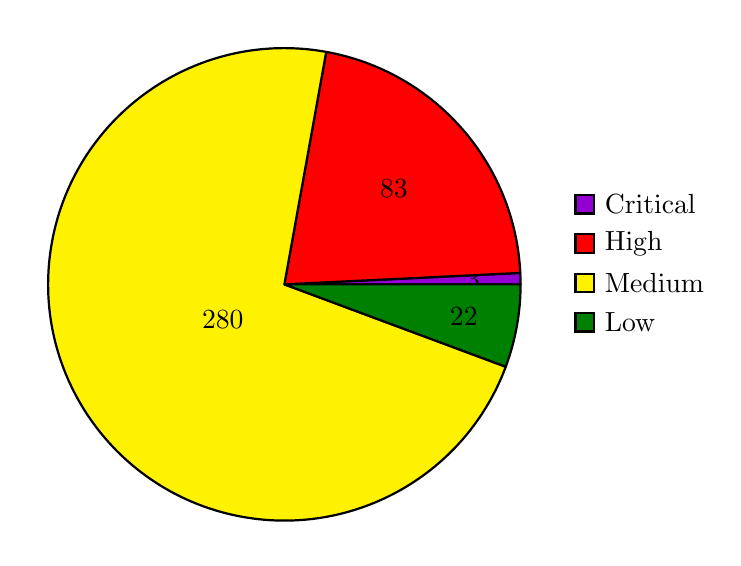
\begin{tikzpicture}
        \pie[
            color={darkviolet, red, yellow, darkgreen},
            text=legend,
            radius=3,
            sum=388
        ]
        {
            3/Critical,
            83/High,
            280/Medium,
            22/Low
        }
    \end{tikzpicture}
\end{figure}


\clearpage

\section{Vulnerability Summary per IP}

\noindent The table below shows the number of critical, high, medium, and low vulnerabilities for each IP, ordered by the number of vulnerabilities (first by critical, then high, medium, and low):

\begin{longtable}{|>{\raggedright\arraybackslash}p{3cm}|c|c|c|c|}
    \hline
    \textbf{IP Address} & \textbf{Critical} & \textbf{High} & \textbf{Medium} & \textbf{Low} \\
    \hline
    \endfirsthead
    \hline
    \textbf{IP Address} & \textbf{Critical} & \textbf{High} & \textbf{Medium} & \textbf{Low} \\
    \hline
    \endhead
    \hline
    \endfoot
    \endlastfoot
    
    
    
    \rowcolor{lightred} % Righe con critical o high evidenziate in rosso
    
    34.242.149.90 & 2 & 9 & 36 & 2 \\
    \hline
    
    
    \rowcolor{lightred} % Righe con critical o high evidenziate in rosso
    
    212.35.217.197 & 1 & 0 & 6 & 1 \\
    \hline
    
    
    \rowcolor{lightred} % Righe con critical o high evidenziate in rosso
    
    80.211.62.104 & 0 & 22 & 94 & 8 \\
    \hline
    
    
    \rowcolor{lightred} % Righe con critical o high evidenziate in rosso
    
    54.220.186.7 & 0 & 16 & 20 & 0 \\
    \hline
    
    
    \rowcolor{lightred} % Righe con critical o high evidenziate in rosso
    
    52.16.137.238 & 0 & 12 & 30 & 4 \\
    \hline
    
    
    \rowcolor{lightred} % Righe con critical o high evidenziate in rosso
    
    109.168.115.125 & 0 & 11 & 60 & 5 \\
    \hline
    
    
    \rowcolor{lightred} % Righe con critical o high evidenziate in rosso
    
    52.17.142.196 & 0 & 6 & 15 & 2 \\
    \hline
    
    
    \rowcolor{lightred} % Righe con critical o high evidenziate in rosso
    
    63.33.34.226 & 0 & 6 & 6 & 0 \\
    \hline
    
    
    \rowcolor{lightred} % Righe con critical o high evidenziate in rosso
    
    54.171.29.175 & 0 & 1 & 1 & 0 \\
    \hline
    
    
    \rowcolor{lightyellow} % Righe con medium o low evidenziate in giallo
    
    34.240.71.165 & 0 & 0 & 6 & 0 \\
    \hline
    
    
    \rowcolor{lightyellow} % Righe con medium o low evidenziate in giallo
    
    52.211.9.207 & 0 & 0 & 4 & 0 \\
    \hline
    
    
    \rowcolor{lightyellow} % Righe con medium o low evidenziate in giallo
    
    151.11.251.115 & 0 & 0 & 1 & 0 \\
    \hline
    
    
    \rowcolor{lightyellow} % Righe con medium o low evidenziate in giallo
    
    151.11.251.108 & 0 & 0 & 1 & 0 \\
    \hline
    
    
    \rowcolor{lightgreen} % Righe senza vulnerabilità evidenziate in verde
    
    54.73.124.6 & 0 & 0 & 0 & 0 \\
    \hline
    
    
    \rowcolor{lightgreen} % Righe senza vulnerabilità evidenziate in verde
    
    52.210.69.61 & 0 & 0 & 0 & 0 \\
    \hline
    
    
    \rowcolor{lightgreen} % Righe senza vulnerabilità evidenziate in verde
    
    109.68.24.219 & 0 & 0 & 0 & 0 \\
    \hline
    
    
    \rowcolor{lightgreen} % Righe senza vulnerabilità evidenziate in verde
    
    34.255.210.70 & 0 & 0 & 0 & 0 \\
    \hline
    
    
    \rowcolor{lightgreen} % Righe senza vulnerabilità evidenziate in verde
    
    52.101.73.21 & 0 & 0 & 0 & 0 \\
    \hline
    
    
    \rowcolor{lightgreen} % Righe senza vulnerabilità evidenziate in verde
    
    109.68.26.97 & 0 & 0 & 0 & 0 \\
    \hline
    
    
    \rowcolor{lightgreen} % Righe senza vulnerabilità evidenziate in verde
    
    52.49.3.128 & 0 & 0 & 0 & 0 \\
    \hline
    
    
    \rowcolor{lightgreen} % Righe senza vulnerabilità evidenziate in verde
    
    52.48.120.101 & 0 & 0 & 0 & 0 \\
    \hline
    
    
    \rowcolor{lightgreen} % Righe senza vulnerabilità evidenziate in verde
    
    34.249.245.96 & 0 & 0 & 0 & 0 \\
    \hline
    
    
    \rowcolor{lightgreen} % Righe senza vulnerabilità evidenziate in verde
    
    52.51.238.226 & 0 & 0 & 0 & 0 \\
    \hline
    
    
    \rowcolor{lightgreen} % Righe senza vulnerabilità evidenziate in verde
    
    63.32.7.7 & 0 & 0 & 0 & 0 \\
    \hline
    
    
    \rowcolor{lightgreen} % Righe senza vulnerabilità evidenziate in verde
    
    151.101.67.10 & 0 & 0 & 0 & 0 \\
    \hline
    
    
    \rowcolor{lightgreen} % Righe senza vulnerabilità evidenziate in verde
    
    52.50.88.161 & 0 & 0 & 0 & 0 \\
    \hline
    
    
    \rowcolor{lightgreen} % Righe senza vulnerabilità evidenziate in verde
    
    52.210.104.122 & 0 & 0 & 0 & 0 \\
    \hline
    
    
    \rowcolor{lightgreen} % Righe senza vulnerabilità evidenziate in verde
    
    52.50.84.159 & 0 & 0 & 0 & 0 \\
    \hline
    
    
    \rowcolor{lightgreen} % Righe senza vulnerabilità evidenziate in verde
    
    159.65.113.205 & 0 & 0 & 0 & 0 \\
    \hline
    
    
    \rowcolor{lightgreen} % Righe senza vulnerabilità evidenziate in verde
    
    52.101.73.11 & 0 & 0 & 0 & 0 \\
    \hline
    
    
    \rowcolor{lightgreen} % Righe senza vulnerabilità evidenziate in verde
    
    35.233.86.30 & 0 & 0 & 0 & 0 \\
    \hline
    
    
    \rowcolor{lightgreen} % Righe senza vulnerabilità evidenziate in verde
    
    151.0.185.49 & 0 & 0 & 0 & 0 \\
    \hline
    
    
    \rowcolor{lightgreen} % Righe senza vulnerabilità evidenziate in verde
    
    185.127.134.97 & 0 & 0 & 0 & 0 \\
    \hline
    
    
    \rowcolor{lightgreen} % Righe senza vulnerabilità evidenziate in verde
    
    109.68.26.86 & 0 & 0 & 0 & 0 \\
    \hline
    
    
    \rowcolor{lightgreen} % Righe senza vulnerabilità evidenziate in verde
    
    34.253.26.23 & 0 & 0 & 0 & 0 \\
    \hline
    
    
    \rowcolor{lightgreen} % Righe senza vulnerabilità evidenziate in verde
    
    52.213.179.200 & 0 & 0 & 0 & 0 \\
    \hline
    
    
    \rowcolor{lightgreen} % Righe senza vulnerabilità evidenziate in verde
    
    54.75.85.203 & 0 & 0 & 0 & 0 \\
    \hline
    
    
    \rowcolor{lightgreen} % Righe senza vulnerabilità evidenziate in verde
    
    52.213.192.243 & 0 & 0 & 0 & 0 \\
    \hline
    
    
    \rowcolor{lightgreen} % Righe senza vulnerabilità evidenziate in verde
    
    52.51.67.222 & 0 & 0 & 0 & 0 \\
    \hline
    
    
    \rowcolor{lightgreen} % Righe senza vulnerabilità evidenziate in verde
    
    54.154.197.101 & 0 & 0 & 0 & 0 \\
    \hline
    
    
    \rowcolor{lightgreen} % Righe senza vulnerabilità evidenziate in verde
    
    151.101.131.10 & 0 & 0 & 0 & 0 \\
    \hline
    
    
    \rowcolor{lightgreen} % Righe senza vulnerabilità evidenziate in verde
    
    63.32.26.88 & 0 & 0 & 0 & 0 \\
    \hline
    
    
    \rowcolor{lightgreen} % Righe senza vulnerabilità evidenziate in verde
    
    79.125.61.213 & 0 & 0 & 0 & 0 \\
    \hline
    
    
    \rowcolor{lightgreen} % Righe senza vulnerabilità evidenziate in verde
    
    99.81.195.173 & 0 & 0 & 0 & 0 \\
    \hline
    
    
    \rowcolor{lightgreen} % Righe senza vulnerabilità evidenziate in verde
    
    63.140.62.27 & 0 & 0 & 0 & 0 \\
    \hline
    
    
    \rowcolor{lightgreen} % Righe senza vulnerabilità evidenziate in verde
    
    52.210.221.125 & 0 & 0 & 0 & 0 \\
    \hline
    
    
    \rowcolor{lightgreen} % Righe senza vulnerabilità evidenziate in verde
    
    99.80.6.39 & 0 & 0 & 0 & 0 \\
    \hline
    
    
    \rowcolor{lightgreen} % Righe senza vulnerabilità evidenziate in verde
    
    52.31.137.103 & 0 & 0 & 0 & 0 \\
    \hline
    
    
    \rowcolor{lightgreen} % Righe senza vulnerabilità evidenziate in verde
    
    52.101.73.24 & 0 & 0 & 0 & 0 \\
    \hline
    
    
    \rowcolor{lightgreen} % Righe senza vulnerabilità evidenziate in verde
    
    63.32.160.121 & 0 & 0 & 0 & 0 \\
    \hline
    
    
    \rowcolor{lightgreen} % Righe senza vulnerabilità evidenziate in verde
    
    193.240.211.109 & 0 & 0 & 0 & 0 \\
    \hline
    
    
    \rowcolor{lightgreen} % Righe senza vulnerabilità evidenziate in verde
    
    52.213.125.100 & 0 & 0 & 0 & 0 \\
    \hline
    
    
    \rowcolor{lightgreen} % Righe senza vulnerabilità evidenziate in verde
    
    54.220.30.149 & 0 & 0 & 0 & 0 \\
    \hline
    
    
    \rowcolor{lightgreen} % Righe senza vulnerabilità evidenziate in verde
    
    52.48.246.2 & 0 & 0 & 0 & 0 \\
    \hline
    
    
    \rowcolor{lightgreen} % Righe senza vulnerabilità evidenziate in verde
    
    54.76.88.210 & 0 & 0 & 0 & 0 \\
    \hline
    
    
    \rowcolor{lightgreen} % Righe senza vulnerabilità evidenziate in verde
    
    54.220.187.182 & 0 & 0 & 0 & 0 \\
    \hline
    
    
    \rowcolor{lightgreen} % Righe senza vulnerabilità evidenziate in verde
    
    52.101.68.36 & 0 & 0 & 0 & 0 \\
    \hline
    
    
    \rowcolor{lightgreen} % Righe senza vulnerabilità evidenziate in verde
    
    34.254.16.163 & 0 & 0 & 0 & 0 \\
    \hline
    
    
    \rowcolor{lightgreen} % Righe senza vulnerabilità evidenziate in verde
    
    165.22.20.19 & 0 & 0 & 0 & 0 \\
    \hline
    
    
    \rowcolor{lightgreen} % Righe senza vulnerabilità evidenziate in verde
    
    54.220.116.192 & 0 & 0 & 0 & 0 \\
    \hline
    
    
    \rowcolor{lightgreen} % Righe senza vulnerabilità evidenziate in verde
    
    52.31.208.124 & 0 & 0 & 0 & 0 \\
    \hline
    
    
    \rowcolor{lightgreen} % Righe senza vulnerabilità evidenziate in verde
    
    151.101.3.10 & 0 & 0 & 0 & 0 \\
    \hline
    
    
    \rowcolor{lightgreen} % Righe senza vulnerabilità evidenziate in verde
    
    34.241.245.151 & 0 & 0 & 0 & 0 \\
    \hline
    
    
    \rowcolor{lightgreen} % Righe senza vulnerabilità evidenziate in verde
    
    52.50.105.114 & 0 & 0 & 0 & 0 \\
    \hline
    
    
    \rowcolor{lightgreen} % Righe senza vulnerabilità evidenziate in verde
    
    213.171.166.88 & 0 & 0 & 0 & 0 \\
    \hline
    
    
    \rowcolor{lightgreen} % Righe senza vulnerabilità evidenziate in verde
    
    54.194.42.165 & 0 & 0 & 0 & 0 \\
    \hline
    
    
    \rowcolor{lightgreen} % Righe senza vulnerabilità evidenziate in verde
    
    54.170.100.107 & 0 & 0 & 0 & 0 \\
    \hline
    
    
    \rowcolor{lightgreen} % Righe senza vulnerabilità evidenziate in verde
    
    54.78.116.130 & 0 & 0 & 0 & 0 \\
    \hline
    
    
    \rowcolor{lightgreen} % Righe senza vulnerabilità evidenziate in verde
    
    151.101.195.10 & 0 & 0 & 0 & 0 \\
    \hline
    
    
    \rowcolor{lightgreen} % Righe senza vulnerabilità evidenziate in verde
    
    217.29.160.31 & 0 & 0 & 0 & 0 \\
    \hline
    
    
    \rowcolor{lightgreen} % Righe senza vulnerabilità evidenziate in verde
    
    3.248.134.241 & 0 & 0 & 0 & 0 \\
    \hline
    
    
    \rowcolor{lightgreen} % Righe senza vulnerabilità evidenziate in verde
    
    116.203.32.52 & 0 & 0 & 0 & 0 \\
    \hline
    
    
    \rowcolor{lightgreen} % Righe senza vulnerabilità evidenziate in verde
    
    52.213.201.198 & 0 & 0 & 0 & 0 \\
    \hline
    
    
    \rowcolor{lightgreen} % Righe senza vulnerabilità evidenziate in verde
    
    34.241.181.233 & 0 & 0 & 0 & 0 \\
    \hline
    
    
    \rowcolor{lightgreen} % Righe senza vulnerabilità evidenziate in verde
    
    54.72.34.250 & 0 & 0 & 0 & 0 \\
    \hline
    
    \caption{Number of vulnerabilities per IP, sorted by severity.} \\
\end{longtable}

\clearpage

\section{Shodan Results for IP Addresses}

Below is the detailed report of vulnerabilities and services for each IP address:



\subsection{IP Address: 54.73.124.6}

\begin{itemize}
    \item \textbf{Organization}: Amazon.com, Inc.
    \item \textbf{Operating System}:  N/A 
    \item \textbf{Critical Vulnerabilities}: 0
    \item \textbf{High Vulnerabilities}: 0
    \item \textbf{Medium Vulnerabilities}: 0
    \item \textbf{Low Vulnerabilities}: 0
    \item \textbf{Total Vulnerabilities}: 0
\end{itemize}

\subsubsection*{Services Running on IP Address}

\begin{itemize}
    
        \item \textbf{Service}: AWS ELB
        \begin{itemize}
            \item \textbf{Port}: 80
            \item \textbf{Version}:  2.0 
            \item \textbf{Location}: \href{ https://54.73.124.6:443/ }{ https://54.73.124.6:443/ }
        \end{itemize}
    
\end{itemize}


\textbf{No vulnerabilities found for this IP address.}




\clearpage



\subsection{IP Address: 52.16.137.238}

\begin{itemize}
    \item \textbf{Organization}: Amazon Data Services Ireland Limited
    \item \textbf{Operating System}:  N/A 
    \item \textbf{Critical Vulnerabilities}: 0
    \item \textbf{High Vulnerabilities}: 12
    \item \textbf{Medium Vulnerabilities}: 30
    \item \textbf{Low Vulnerabilities}: 4
    \item \textbf{Total Vulnerabilities}: 46
\end{itemize}

\subsubsection*{Services Running on IP Address}

\begin{itemize}
    
        \item \textbf{Service}: Apache httpd
        \begin{itemize}
            \item \textbf{Port}: 80
            \item \textbf{Version}:  2.4.52 
            \item \textbf{Location}: \href{ / }{ / }
        \end{itemize}
    
        \item \textbf{Service}: Apache httpd
        \begin{itemize}
            \item \textbf{Port}: 443
            \item \textbf{Version}:  2.4.52 
            \item \textbf{Location}: \href{ / }{ / }
        \end{itemize}
    
\end{itemize}


\subsubsection*{Vulnerabilities Found}

\begin{itemize}
    
        \item \textbf{Vulnerability}: CVE-2024-27316
        \begin{itemize}
            \item \textbf{CVSS Score}:  N/A 
            \item \textbf{Description}:
            \parbox[t]{0.9\linewidth}{
                \ttfamily HTTP/2 incoming headers exceeding the limit are temporarily buffered in nghttp2 in order to generate an informative HTTP 413 response. If a client does not stop sending headers, this leads to memory exhaustion.
            }
        \end{itemize}
    
        \item \textbf{Vulnerability}: CVE-2013-2765
        \begin{itemize}
            \item \textbf{CVSS Score}:  5 
            \item \textbf{Description}:
            \parbox[t]{0.9\linewidth}{
                \ttfamily The ModSecurity module before 2.7.4 for the Apache HTTP Server allows remote attackers to cause a denial of service (NULL pointer dereference, process crash, and disk consumption) via a POST request with a large body and a crafted Content-Type header.
            }
        \end{itemize}
    
        \item \textbf{Vulnerability}: CVE-2022-36760
        \begin{itemize}
            \item \textbf{CVSS Score}:  N/A 
            \item \textbf{Description}:
            \parbox[t]{0.9\linewidth}{
                \ttfamily Inconsistent Interpretation of HTTP Requests ('HTTP Request Smuggling') vulnerability in mod\_proxy\_ajp of Apache HTTP Server allows an attacker to smuggle requests to the AJP server it forwards requests to.  This issue affects Apache HTTP Server Apache HTTP Server 2.4 version 2.4.54 and prior versions.
            }
        \end{itemize}
    
        \item \textbf{Vulnerability}: CVE-2022-29404
        \begin{itemize}
            \item \textbf{CVSS Score}:  5 
            \item \textbf{Description}:
            \parbox[t]{0.9\linewidth}{
                \ttfamily In Apache HTTP Server 2.4.53 and earlier, a malicious request to a lua script that calls r:parsebody(0) may cause a denial of service due to no default limit on possible input size.
            }
        \end{itemize}
    
        \item \textbf{Vulnerability}: CVE-2023-27522
        \begin{itemize}
            \item \textbf{CVSS Score}:  N/A 
            \item \textbf{Description}:
            \parbox[t]{0.9\linewidth}{
                \ttfamily HTTP Response Smuggling vulnerability in Apache HTTP Server via mod\_proxy\_uwsgi. This issue affects Apache HTTP Server: from 2.4.30 through 2.4.55.Special characters in the origin response header can truncate/split the response forwarded to the client.
            }
        \end{itemize}
    
        \item \textbf{Vulnerability}: CVE-2013-4365
        \begin{itemize}
            \item \textbf{CVSS Score}:  7.5 
            \item \textbf{Description}:
            \parbox[t]{0.9\linewidth}{
                \ttfamily Heap-based buffer overflow in the fcgid\_header\_bucket\_read function in fcgid\_bucket.c in the mod\_fcgid module before 2.3.9 for the Apache HTTP Server allows remote attackers to have an unspecified impact via unknown vectors.
            }
        \end{itemize}
    
        \item \textbf{Vulnerability}: CVE-2022-22720
        \begin{itemize}
            \item \textbf{CVSS Score}:  7.5 
            \item \textbf{Description}:
            \parbox[t]{0.9\linewidth}{
                \ttfamily Apache HTTP Server 2.4.52 and earlier fails to close inbound connection when errors are encountered discarding the request body, exposing the server to HTTP Request Smuggling
            }
        \end{itemize}
    
        \item \textbf{Vulnerability}: CVE-2022-28330
        \begin{itemize}
            \item \textbf{CVSS Score}:  5 
            \item \textbf{Description}:
            \parbox[t]{0.9\linewidth}{
                \ttfamily Apache HTTP Server 2.4.53 and earlier on Windows may read beyond bounds when configured to process requests with the mod\_isapi module.
            }
        \end{itemize}
    
        \item \textbf{Vulnerability}: CVE-2023-31122
        \begin{itemize}
            \item \textbf{CVSS Score}:  N/A 
            \item \textbf{Description}:
            \parbox[t]{0.9\linewidth}{
                \ttfamily Out-of-bounds Read vulnerability in mod\_macro of Apache HTTP Server.This issue affects Apache HTTP Server: through 2.4.57.
            }
        \end{itemize}
    
        \item \textbf{Vulnerability}: CVE-2024-38476
        \begin{itemize}
            \item \textbf{CVSS Score}:  N/A 
            \item \textbf{Description}:
            \parbox[t]{0.9\linewidth}{
                \ttfamily Vulnerability in core of Apache HTTP Server 2.4.59 and earlier are vulnerably to information disclosure, SSRF or local script execution viabackend applications whose response headers are malicious or exploitable.Users are recommended to upgrade to version 2.4.60, which fixes this issue.
            }
        \end{itemize}
    
        \item \textbf{Vulnerability}: CVE-2024-38477
        \begin{itemize}
            \item \textbf{CVSS Score}:  N/A 
            \item \textbf{Description}:
            \parbox[t]{0.9\linewidth}{
                \ttfamily null pointer dereference in mod\_proxy in Apache HTTP Server 2.4.59 and earlier allows an attacker to crash the server via a malicious request.Users are recommended to upgrade to version 2.4.60, which fixes this issue.
            }
        \end{itemize}
    
        \item \textbf{Vulnerability}: CVE-2024-38474
        \begin{itemize}
            \item \textbf{CVSS Score}:  N/A 
            \item \textbf{Description}:
            \parbox[t]{0.9\linewidth}{
                \ttfamily Substitution encoding issue in mod\_rewrite in Apache HTTP Server 2.4.59 and earlier allows attacker to execute scripts indirectories permitted by the configuration but not directly reachable by anyURL or source disclosure of scripts meant to only to be executed as CGI.Users are recommended to upgrade to version 2.4.60, which fixes this issue.Some RewriteRules that capture and substitute unsafely will now fail unless rewrite flag "UnsafeAllow3F" is specified.
            }
        \end{itemize}
    
        \item \textbf{Vulnerability}: CVE-2022-22721
        \begin{itemize}
            \item \textbf{CVSS Score}:  5.8 
            \item \textbf{Description}:
            \parbox[t]{0.9\linewidth}{
                \ttfamily If LimitXMLRequestBody is set to allow request bodies larger than 350MB (defaults to 1M) on 32 bit systems an integer overflow happens which later causes out of bounds writes. This issue affects Apache HTTP Server 2.4.52 and earlier.
            }
        \end{itemize}
    
        \item \textbf{Vulnerability}: CVE-2006-20001
        \begin{itemize}
            \item \textbf{CVSS Score}:  N/A 
            \item \textbf{Description}:
            \parbox[t]{0.9\linewidth}{
                \ttfamily A carefully crafted If: request header can cause a memory read, or write of a single zero byte, in a pool (heap) memory location beyond the header value sent. This could cause the process to crash.This issue affects Apache HTTP Server 2.4.54 and earlier.
            }
        \end{itemize}
    
        \item \textbf{Vulnerability}: CVE-2009-0796
        \begin{itemize}
            \item \textbf{CVSS Score}:  2.6 
            \item \textbf{Description}:
            \parbox[t]{0.9\linewidth}{
                \ttfamily Cross-site scripting (XSS) vulnerability in Status.pm in Apache::Status and Apache2::Status in mod\_perl1 and mod\_perl2 for the Apache HTTP Server, when /perl-status is accessible, allows remote attackers to inject arbitrary web script or HTML via the URI.
            }
        \end{itemize}
    
        \item \textbf{Vulnerability}: CVE-2012-3526
        \begin{itemize}
            \item \textbf{CVSS Score}:  5 
            \item \textbf{Description}:
            \parbox[t]{0.9\linewidth}{
                \ttfamily The reverse proxy add forward module (mod\_rpaf) 0.5 and 0.6 for the Apache HTTP Server allows remote attackers to cause a denial of service (server or application crash) via multiple X-Forwarded-For headers in a request.
            }
        \end{itemize}
    
        \item \textbf{Vulnerability}: CVE-2022-31813
        \begin{itemize}
            \item \textbf{CVSS Score}:  7.5 
            \item \textbf{Description}:
            \parbox[t]{0.9\linewidth}{
                \ttfamily Apache HTTP Server 2.4.53 and earlier may not send the X-Forwarded-* headers to the origin server based on client side Connection header hop-by-hop mechanism. This may be used to bypass IP based authentication on the origin server/application.
            }
        \end{itemize}
    
        \item \textbf{Vulnerability}: CVE-2012-4001
        \begin{itemize}
            \item \textbf{CVSS Score}:  5 
            \item \textbf{Description}:
            \parbox[t]{0.9\linewidth}{
                \ttfamily The mod\_pagespeed module before 0.10.22.6 for the Apache HTTP Server does not properly verify its host name, which allows remote attackers to trigger HTTP requests to arbitrary hosts via unspecified vectors, as demonstrated by requests to intranet servers.
            }
        \end{itemize}
    
        \item \textbf{Vulnerability}: CVE-2022-37436
        \begin{itemize}
            \item \textbf{CVSS Score}:  N/A 
            \item \textbf{Description}:
            \parbox[t]{0.9\linewidth}{
                \ttfamily Prior to Apache HTTP Server 2.4.55, a malicious backend can cause the response headers to be truncated early, resulting in some headers being incorporated into the response body. If the later headers have any security purpose, they will not be interpreted by the client.
            }
        \end{itemize}
    
        \item \textbf{Vulnerability}: CVE-2012-4360
        \begin{itemize}
            \item \textbf{CVSS Score}:  4.3 
            \item \textbf{Description}:
            \parbox[t]{0.9\linewidth}{
                \ttfamily Cross-site scripting (XSS) vulnerability in the mod\_pagespeed module 0.10.19.1 through 0.10.22.4 for the Apache HTTP Server allows remote attackers to inject arbitrary web script or HTML via unspecified vectors.
            }
        \end{itemize}
    
        \item \textbf{Vulnerability}: CVE-2011-1176
        \begin{itemize}
            \item \textbf{CVSS Score}:  4.3 
            \item \textbf{Description}:
            \parbox[t]{0.9\linewidth}{
                \ttfamily The configuration merger in itk.c in the Steinar H. Gunderson mpm-itk Multi-Processing Module 2.2.11-01 and 2.2.11-02 for the Apache HTTP Server does not properly handle certain configuration sections that specify NiceValue but not AssignUserID, which might allow remote attackers to gain privileges by leveraging the root uid and root gid of an mpm-itk process.
            }
        \end{itemize}
    
        \item \textbf{Vulnerability}: CVE-2022-23943
        \begin{itemize}
            \item \textbf{CVSS Score}:  7.5 
            \item \textbf{Description}:
            \parbox[t]{0.9\linewidth}{
                \ttfamily Out-of-bounds Write vulnerability in mod\_sed of Apache HTTP Server allows an attacker to overwrite heap memory with possibly attacker provided data. This issue affects Apache HTTP Server 2.4 version 2.4.52 and prior versions.
            }
        \end{itemize}
    
        \item \textbf{Vulnerability}: CVE-2011-2688
        \begin{itemize}
            \item \textbf{CVSS Score}:  7.5 
            \item \textbf{Description}:
            \parbox[t]{0.9\linewidth}{
                \ttfamily SQL injection vulnerability in mysql/mysql-auth.pl in the mod\_authnz\_external module 3.2.5 and earlier for the Apache HTTP Server allows remote attackers to execute arbitrary SQL commands via the user field.
            }
        \end{itemize}
    
        \item \textbf{Vulnerability}: CVE-2023-25690
        \begin{itemize}
            \item \textbf{CVSS Score}:  N/A 
            \item \textbf{Description}:
            \parbox[t]{0.9\linewidth}{
                \ttfamily Some mod\_proxy configurations on Apache HTTP Server versions 2.4.0 through 2.4.55 allow a HTTP Request Smuggling attack.Configurations are affected when mod\_proxy is enabled along with some form of RewriteRule or ProxyPassMatch in which a non-specific pattern matches some portion of the user-supplied request-target (URL) data and is then re-inserted into the proxied request-target using variable substitution. For example, something like:RewriteEngine onRewriteRule "\^/here/(.*)" "http://example.com:8080/elsewhere?\$1"; [P]ProxyPassReverse /here/ http://example.com:8080/Request splitting/smuggling could result in bypass of access controls in the proxy server, proxying unintended URLs to existing origin servers, and cache poisoning. Users are recommended to update to at least version 2.4.56 of Apache HTTP Server.
            }
        \end{itemize}
    
        \item \textbf{Vulnerability}: CVE-2007-4723
        \begin{itemize}
            \item \textbf{CVSS Score}:  7.5 
            \item \textbf{Description}:
            \parbox[t]{0.9\linewidth}{
                \ttfamily Directory traversal vulnerability in Ragnarok Online Control Panel 4.3.4a, when the Apache HTTP Server is used, allows remote attackers to bypass authentication via directory traversal sequences in a URI that ends with the name of a publicly available page, as demonstrated by a "/...../" sequence and an account\_manage.php/login.php final component for reaching the protected account\_manage.php page.
            }
        \end{itemize}
    
        \item \textbf{Vulnerability}: CVE-2013-0941
        \begin{itemize}
            \item \textbf{CVSS Score}:  2.1 
            \item \textbf{Description}:
            \parbox[t]{0.9\linewidth}{
                \ttfamily EMC RSA Authentication API before 8.1 SP1, RSA Web Agent before 5.3.5 for Apache Web Server, RSA Web Agent before 5.3.5 for IIS, RSA PAM Agent before 7.0, and RSA Agent before 6.1.4 for Microsoft Windows use an improper encryption algorithm and a weak key for maintaining the stored data of the node secret for the SecurID Authentication API, which allows local users to obtain sensitive information via cryptographic attacks on this data.
            }
        \end{itemize}
    
        \item \textbf{Vulnerability}: CVE-2013-0942
        \begin{itemize}
            \item \textbf{CVSS Score}:  4.3 
            \item \textbf{Description}:
            \parbox[t]{0.9\linewidth}{
                \ttfamily Cross-site scripting (XSS) vulnerability in EMC RSA Authentication Agent 7.1 before 7.1.1 for Web for Internet Information Services, and 7.1 before 7.1.1 for Web for Apache, allows remote attackers to inject arbitrary web script or HTML via unspecified vectors.
            }
        \end{itemize}
    
        \item \textbf{Vulnerability}: CVE-2022-26377
        \begin{itemize}
            \item \textbf{CVSS Score}:  5 
            \item \textbf{Description}:
            \parbox[t]{0.9\linewidth}{
                \ttfamily Inconsistent Interpretation of HTTP Requests ('HTTP Request Smuggling') vulnerability in mod\_proxy\_ajp of Apache HTTP Server allows an attacker to smuggle requests to the AJP server it forwards requests to. This issue affects Apache HTTP Server Apache HTTP Server 2.4 version 2.4.53 and prior versions.
            }
        \end{itemize}
    
        \item \textbf{Vulnerability}: CVE-2023-45802
        \begin{itemize}
            \item \textbf{CVSS Score}:  N/A 
            \item \textbf{Description}:
            \parbox[t]{0.9\linewidth}{
                \ttfamily When a HTTP/2 stream was reset (RST frame) by a client, there was a time window were the request's memory resources were not reclaimed immediately. Instead, de-allocation was deferred to connection close. A client could send new requests and resets, keeping the connection busy and open and causing the memory footprint to keep on growing. On connection close, all resources were reclaimed, but the process might run out of memory before that.This was found by the reporter during testing ofCVE-2023-44487 (HTTP/2 Rapid Reset Exploit) with their own test client. During "normal" HTTP/2 use, the probability to hit this bug is very low. The kept memory would not become noticeable before the connection closes or times out.Users are recommended to upgrade to version 2.4.58, which fixes the issue.
            }
        \end{itemize}
    
        \item \textbf{Vulnerability}: CVE-2022-28614
        \begin{itemize}
            \item \textbf{CVSS Score}:  5 
            \item \textbf{Description}:
            \parbox[t]{0.9\linewidth}{
                \ttfamily The ap\_rwrite() function in Apache HTTP Server 2.4.53 and earlier may read unintended memory if an attacker can cause the server to reflect very large input using ap\_rwrite() or ap\_rputs(), such as with mod\_luas r:puts() function. Modules compiled and distributed separately from Apache HTTP Server that use the 'ap\_rputs' function and may pass it a very large (INT\_MAX or larger) string must be compiled against current headers to resolve the issue.
            }
        \end{itemize}
    
        \item \textbf{Vulnerability}: CVE-2009-2299
        \begin{itemize}
            \item \textbf{CVSS Score}:  5 
            \item \textbf{Description}:
            \parbox[t]{0.9\linewidth}{
                \ttfamily The Artofdefence Hyperguard Web Application Firewall (WAF) module before 2.5.5-11635, 3.0 before 3.0.3-11636, and 3.1 before 3.1.1-11637, a module for the Apache HTTP Server, allows remote attackers to cause a denial of service (memory consumption) via an HTTP request with a large Content-Length value but no POST data.
            }
        \end{itemize}
    
        \item \textbf{Vulnerability}: CVE-2024-40898
        \begin{itemize}
            \item \textbf{CVSS Score}:  N/A 
            \item \textbf{Description}:
            \parbox[t]{0.9\linewidth}{
                \ttfamily SSRF in Apache HTTP Server on Windows with mod\_rewrite in server/vhost context, allows to potentially leak NTML hashes to a malicious server via SSRF and malicious requests.Users are recommended to upgrade to version 2.4.62 which fixes this issue.
            }
        \end{itemize}
    
        \item \textbf{Vulnerability}: CVE-2022-28615
        \begin{itemize}
            \item \textbf{CVSS Score}:  6.4 
            \item \textbf{Description}:
            \parbox[t]{0.9\linewidth}{
                \ttfamily Apache HTTP Server 2.4.53 and earlier may crash or disclose information due to a read beyond bounds in ap\_strcmp\_match() when provided with an extremely large input buffer. While no code distributed with the server can be coerced into such a call, third-party modules or lua scripts that use ap\_strcmp\_match() may hypothetically be affected.
            }
        \end{itemize}
    
        \item \textbf{Vulnerability}: CVE-2022-30556
        \begin{itemize}
            \item \textbf{CVSS Score}:  5 
            \item \textbf{Description}:
            \parbox[t]{0.9\linewidth}{
                \ttfamily Apache HTTP Server 2.4.53 and earlier may return lengths to applications calling r:wsread() that point past the end of the storage allocated for the buffer.
            }
        \end{itemize}
    
        \item \textbf{Vulnerability}: CVE-2022-22719
        \begin{itemize}
            \item \textbf{CVSS Score}:  5 
            \item \textbf{Description}:
            \parbox[t]{0.9\linewidth}{
                \ttfamily A carefully crafted request body can cause a read to a random memory area which could cause the process to crash. This issue affects Apache HTTP Server 2.4.52 and earlier.
            }
        \end{itemize}
    
        \item \textbf{Vulnerability}: CVE-2024-27316
        \begin{itemize}
            \item \textbf{CVSS Score}:  N/A 
            \item \textbf{Description}:
            \parbox[t]{0.9\linewidth}{
                \ttfamily HTTP/2 incoming headers exceeding the limit are temporarily buffered in nghttp2 in order to generate an informative HTTP 413 response. If a client does not stop sending headers, this leads to memory exhaustion.
            }
        \end{itemize}
    
        \item \textbf{Vulnerability}: CVE-2013-2765
        \begin{itemize}
            \item \textbf{CVSS Score}:  5 
            \item \textbf{Description}:
            \parbox[t]{0.9\linewidth}{
                \ttfamily The ModSecurity module before 2.7.4 for the Apache HTTP Server allows remote attackers to cause a denial of service (NULL pointer dereference, process crash, and disk consumption) via a POST request with a large body and a crafted Content-Type header.
            }
        \end{itemize}
    
        \item \textbf{Vulnerability}: CVE-2022-36760
        \begin{itemize}
            \item \textbf{CVSS Score}:  N/A 
            \item \textbf{Description}:
            \parbox[t]{0.9\linewidth}{
                \ttfamily Inconsistent Interpretation of HTTP Requests ('HTTP Request Smuggling') vulnerability in mod\_proxy\_ajp of Apache HTTP Server allows an attacker to smuggle requests to the AJP server it forwards requests to.  This issue affects Apache HTTP Server Apache HTTP Server 2.4 version 2.4.54 and prior versions.
            }
        \end{itemize}
    
        \item \textbf{Vulnerability}: CVE-2022-29404
        \begin{itemize}
            \item \textbf{CVSS Score}:  5 
            \item \textbf{Description}:
            \parbox[t]{0.9\linewidth}{
                \ttfamily In Apache HTTP Server 2.4.53 and earlier, a malicious request to a lua script that calls r:parsebody(0) may cause a denial of service due to no default limit on possible input size.
            }
        \end{itemize}
    
        \item \textbf{Vulnerability}: CVE-2023-27522
        \begin{itemize}
            \item \textbf{CVSS Score}:  N/A 
            \item \textbf{Description}:
            \parbox[t]{0.9\linewidth}{
                \ttfamily HTTP Response Smuggling vulnerability in Apache HTTP Server via mod\_proxy\_uwsgi. This issue affects Apache HTTP Server: from 2.4.30 through 2.4.55.Special characters in the origin response header can truncate/split the response forwarded to the client.
            }
        \end{itemize}
    
        \item \textbf{Vulnerability}: CVE-2013-4365
        \begin{itemize}
            \item \textbf{CVSS Score}:  7.5 
            \item \textbf{Description}:
            \parbox[t]{0.9\linewidth}{
                \ttfamily Heap-based buffer overflow in the fcgid\_header\_bucket\_read function in fcgid\_bucket.c in the mod\_fcgid module before 2.3.9 for the Apache HTTP Server allows remote attackers to have an unspecified impact via unknown vectors.
            }
        \end{itemize}
    
        \item \textbf{Vulnerability}: CVE-2022-22720
        \begin{itemize}
            \item \textbf{CVSS Score}:  7.5 
            \item \textbf{Description}:
            \parbox[t]{0.9\linewidth}{
                \ttfamily Apache HTTP Server 2.4.52 and earlier fails to close inbound connection when errors are encountered discarding the request body, exposing the server to HTTP Request Smuggling
            }
        \end{itemize}
    
        \item \textbf{Vulnerability}: CVE-2022-28330
        \begin{itemize}
            \item \textbf{CVSS Score}:  5 
            \item \textbf{Description}:
            \parbox[t]{0.9\linewidth}{
                \ttfamily Apache HTTP Server 2.4.53 and earlier on Windows may read beyond bounds when configured to process requests with the mod\_isapi module.
            }
        \end{itemize}
    
        \item \textbf{Vulnerability}: CVE-2023-31122
        \begin{itemize}
            \item \textbf{CVSS Score}:  N/A 
            \item \textbf{Description}:
            \parbox[t]{0.9\linewidth}{
                \ttfamily Out-of-bounds Read vulnerability in mod\_macro of Apache HTTP Server.This issue affects Apache HTTP Server: through 2.4.57.
            }
        \end{itemize}
    
        \item \textbf{Vulnerability}: CVE-2024-38476
        \begin{itemize}
            \item \textbf{CVSS Score}:  N/A 
            \item \textbf{Description}:
            \parbox[t]{0.9\linewidth}{
                \ttfamily Vulnerability in core of Apache HTTP Server 2.4.59 and earlier are vulnerably to information disclosure, SSRF or local script execution viabackend applications whose response headers are malicious or exploitable.Users are recommended to upgrade to version 2.4.60, which fixes this issue.
            }
        \end{itemize}
    
        \item \textbf{Vulnerability}: CVE-2024-38477
        \begin{itemize}
            \item \textbf{CVSS Score}:  N/A 
            \item \textbf{Description}:
            \parbox[t]{0.9\linewidth}{
                \ttfamily null pointer dereference in mod\_proxy in Apache HTTP Server 2.4.59 and earlier allows an attacker to crash the server via a malicious request.Users are recommended to upgrade to version 2.4.60, which fixes this issue.
            }
        \end{itemize}
    
        \item \textbf{Vulnerability}: CVE-2024-38474
        \begin{itemize}
            \item \textbf{CVSS Score}:  N/A 
            \item \textbf{Description}:
            \parbox[t]{0.9\linewidth}{
                \ttfamily Substitution encoding issue in mod\_rewrite in Apache HTTP Server 2.4.59 and earlier allows attacker to execute scripts indirectories permitted by the configuration but not directly reachable by anyURL or source disclosure of scripts meant to only to be executed as CGI.Users are recommended to upgrade to version 2.4.60, which fixes this issue.Some RewriteRules that capture and substitute unsafely will now fail unless rewrite flag "UnsafeAllow3F" is specified.
            }
        \end{itemize}
    
        \item \textbf{Vulnerability}: CVE-2022-22721
        \begin{itemize}
            \item \textbf{CVSS Score}:  5.8 
            \item \textbf{Description}:
            \parbox[t]{0.9\linewidth}{
                \ttfamily If LimitXMLRequestBody is set to allow request bodies larger than 350MB (defaults to 1M) on 32 bit systems an integer overflow happens which later causes out of bounds writes. This issue affects Apache HTTP Server 2.4.52 and earlier.
            }
        \end{itemize}
    
        \item \textbf{Vulnerability}: CVE-2006-20001
        \begin{itemize}
            \item \textbf{CVSS Score}:  N/A 
            \item \textbf{Description}:
            \parbox[t]{0.9\linewidth}{
                \ttfamily A carefully crafted If: request header can cause a memory read, or write of a single zero byte, in a pool (heap) memory location beyond the header value sent. This could cause the process to crash.This issue affects Apache HTTP Server 2.4.54 and earlier.
            }
        \end{itemize}
    
        \item \textbf{Vulnerability}: CVE-2009-0796
        \begin{itemize}
            \item \textbf{CVSS Score}:  2.6 
            \item \textbf{Description}:
            \parbox[t]{0.9\linewidth}{
                \ttfamily Cross-site scripting (XSS) vulnerability in Status.pm in Apache::Status and Apache2::Status in mod\_perl1 and mod\_perl2 for the Apache HTTP Server, when /perl-status is accessible, allows remote attackers to inject arbitrary web script or HTML via the URI.
            }
        \end{itemize}
    
        \item \textbf{Vulnerability}: CVE-2012-3526
        \begin{itemize}
            \item \textbf{CVSS Score}:  5 
            \item \textbf{Description}:
            \parbox[t]{0.9\linewidth}{
                \ttfamily The reverse proxy add forward module (mod\_rpaf) 0.5 and 0.6 for the Apache HTTP Server allows remote attackers to cause a denial of service (server or application crash) via multiple X-Forwarded-For headers in a request.
            }
        \end{itemize}
    
        \item \textbf{Vulnerability}: CVE-2022-31813
        \begin{itemize}
            \item \textbf{CVSS Score}:  7.5 
            \item \textbf{Description}:
            \parbox[t]{0.9\linewidth}{
                \ttfamily Apache HTTP Server 2.4.53 and earlier may not send the X-Forwarded-* headers to the origin server based on client side Connection header hop-by-hop mechanism. This may be used to bypass IP based authentication on the origin server/application.
            }
        \end{itemize}
    
        \item \textbf{Vulnerability}: CVE-2012-4001
        \begin{itemize}
            \item \textbf{CVSS Score}:  5 
            \item \textbf{Description}:
            \parbox[t]{0.9\linewidth}{
                \ttfamily The mod\_pagespeed module before 0.10.22.6 for the Apache HTTP Server does not properly verify its host name, which allows remote attackers to trigger HTTP requests to arbitrary hosts via unspecified vectors, as demonstrated by requests to intranet servers.
            }
        \end{itemize}
    
        \item \textbf{Vulnerability}: CVE-2022-37436
        \begin{itemize}
            \item \textbf{CVSS Score}:  N/A 
            \item \textbf{Description}:
            \parbox[t]{0.9\linewidth}{
                \ttfamily Prior to Apache HTTP Server 2.4.55, a malicious backend can cause the response headers to be truncated early, resulting in some headers being incorporated into the response body. If the later headers have any security purpose, they will not be interpreted by the client.
            }
        \end{itemize}
    
        \item \textbf{Vulnerability}: CVE-2012-4360
        \begin{itemize}
            \item \textbf{CVSS Score}:  4.3 
            \item \textbf{Description}:
            \parbox[t]{0.9\linewidth}{
                \ttfamily Cross-site scripting (XSS) vulnerability in the mod\_pagespeed module 0.10.19.1 through 0.10.22.4 for the Apache HTTP Server allows remote attackers to inject arbitrary web script or HTML via unspecified vectors.
            }
        \end{itemize}
    
        \item \textbf{Vulnerability}: CVE-2011-1176
        \begin{itemize}
            \item \textbf{CVSS Score}:  4.3 
            \item \textbf{Description}:
            \parbox[t]{0.9\linewidth}{
                \ttfamily The configuration merger in itk.c in the Steinar H. Gunderson mpm-itk Multi-Processing Module 2.2.11-01 and 2.2.11-02 for the Apache HTTP Server does not properly handle certain configuration sections that specify NiceValue but not AssignUserID, which might allow remote attackers to gain privileges by leveraging the root uid and root gid of an mpm-itk process.
            }
        \end{itemize}
    
        \item \textbf{Vulnerability}: CVE-2022-23943
        \begin{itemize}
            \item \textbf{CVSS Score}:  7.5 
            \item \textbf{Description}:
            \parbox[t]{0.9\linewidth}{
                \ttfamily Out-of-bounds Write vulnerability in mod\_sed of Apache HTTP Server allows an attacker to overwrite heap memory with possibly attacker provided data. This issue affects Apache HTTP Server 2.4 version 2.4.52 and prior versions.
            }
        \end{itemize}
    
        \item \textbf{Vulnerability}: CVE-2011-2688
        \begin{itemize}
            \item \textbf{CVSS Score}:  7.5 
            \item \textbf{Description}:
            \parbox[t]{0.9\linewidth}{
                \ttfamily SQL injection vulnerability in mysql/mysql-auth.pl in the mod\_authnz\_external module 3.2.5 and earlier for the Apache HTTP Server allows remote attackers to execute arbitrary SQL commands via the user field.
            }
        \end{itemize}
    
        \item \textbf{Vulnerability}: CVE-2023-25690
        \begin{itemize}
            \item \textbf{CVSS Score}:  N/A 
            \item \textbf{Description}:
            \parbox[t]{0.9\linewidth}{
                \ttfamily Some mod\_proxy configurations on Apache HTTP Server versions 2.4.0 through 2.4.55 allow a HTTP Request Smuggling attack.Configurations are affected when mod\_proxy is enabled along with some form of RewriteRule or ProxyPassMatch in which a non-specific pattern matches some portion of the user-supplied request-target (URL) data and is then re-inserted into the proxied request-target using variable substitution. For example, something like:RewriteEngine onRewriteRule "\^/here/(.*)" "http://example.com:8080/elsewhere?\$1"; [P]ProxyPassReverse /here/ http://example.com:8080/Request splitting/smuggling could result in bypass of access controls in the proxy server, proxying unintended URLs to existing origin servers, and cache poisoning. Users are recommended to update to at least version 2.4.56 of Apache HTTP Server.
            }
        \end{itemize}
    
        \item \textbf{Vulnerability}: CVE-2007-4723
        \begin{itemize}
            \item \textbf{CVSS Score}:  7.5 
            \item \textbf{Description}:
            \parbox[t]{0.9\linewidth}{
                \ttfamily Directory traversal vulnerability in Ragnarok Online Control Panel 4.3.4a, when the Apache HTTP Server is used, allows remote attackers to bypass authentication via directory traversal sequences in a URI that ends with the name of a publicly available page, as demonstrated by a "/...../" sequence and an account\_manage.php/login.php final component for reaching the protected account\_manage.php page.
            }
        \end{itemize}
    
        \item \textbf{Vulnerability}: CVE-2013-0941
        \begin{itemize}
            \item \textbf{CVSS Score}:  2.1 
            \item \textbf{Description}:
            \parbox[t]{0.9\linewidth}{
                \ttfamily EMC RSA Authentication API before 8.1 SP1, RSA Web Agent before 5.3.5 for Apache Web Server, RSA Web Agent before 5.3.5 for IIS, RSA PAM Agent before 7.0, and RSA Agent before 6.1.4 for Microsoft Windows use an improper encryption algorithm and a weak key for maintaining the stored data of the node secret for the SecurID Authentication API, which allows local users to obtain sensitive information via cryptographic attacks on this data.
            }
        \end{itemize}
    
        \item \textbf{Vulnerability}: CVE-2013-0942
        \begin{itemize}
            \item \textbf{CVSS Score}:  4.3 
            \item \textbf{Description}:
            \parbox[t]{0.9\linewidth}{
                \ttfamily Cross-site scripting (XSS) vulnerability in EMC RSA Authentication Agent 7.1 before 7.1.1 for Web for Internet Information Services, and 7.1 before 7.1.1 for Web for Apache, allows remote attackers to inject arbitrary web script or HTML via unspecified vectors.
            }
        \end{itemize}
    
        \item \textbf{Vulnerability}: CVE-2022-26377
        \begin{itemize}
            \item \textbf{CVSS Score}:  5 
            \item \textbf{Description}:
            \parbox[t]{0.9\linewidth}{
                \ttfamily Inconsistent Interpretation of HTTP Requests ('HTTP Request Smuggling') vulnerability in mod\_proxy\_ajp of Apache HTTP Server allows an attacker to smuggle requests to the AJP server it forwards requests to. This issue affects Apache HTTP Server Apache HTTP Server 2.4 version 2.4.53 and prior versions.
            }
        \end{itemize}
    
        \item \textbf{Vulnerability}: CVE-2023-45802
        \begin{itemize}
            \item \textbf{CVSS Score}:  N/A 
            \item \textbf{Description}:
            \parbox[t]{0.9\linewidth}{
                \ttfamily When a HTTP/2 stream was reset (RST frame) by a client, there was a time window were the request's memory resources were not reclaimed immediately. Instead, de-allocation was deferred to connection close. A client could send new requests and resets, keeping the connection busy and open and causing the memory footprint to keep on growing. On connection close, all resources were reclaimed, but the process might run out of memory before that.This was found by the reporter during testing ofCVE-2023-44487 (HTTP/2 Rapid Reset Exploit) with their own test client. During "normal" HTTP/2 use, the probability to hit this bug is very low. The kept memory would not become noticeable before the connection closes or times out.Users are recommended to upgrade to version 2.4.58, which fixes the issue.
            }
        \end{itemize}
    
        \item \textbf{Vulnerability}: CVE-2022-28614
        \begin{itemize}
            \item \textbf{CVSS Score}:  5 
            \item \textbf{Description}:
            \parbox[t]{0.9\linewidth}{
                \ttfamily The ap\_rwrite() function in Apache HTTP Server 2.4.53 and earlier may read unintended memory if an attacker can cause the server to reflect very large input using ap\_rwrite() or ap\_rputs(), such as with mod\_luas r:puts() function. Modules compiled and distributed separately from Apache HTTP Server that use the 'ap\_rputs' function and may pass it a very large (INT\_MAX or larger) string must be compiled against current headers to resolve the issue.
            }
        \end{itemize}
    
        \item \textbf{Vulnerability}: CVE-2009-2299
        \begin{itemize}
            \item \textbf{CVSS Score}:  5 
            \item \textbf{Description}:
            \parbox[t]{0.9\linewidth}{
                \ttfamily The Artofdefence Hyperguard Web Application Firewall (WAF) module before 2.5.5-11635, 3.0 before 3.0.3-11636, and 3.1 before 3.1.1-11637, a module for the Apache HTTP Server, allows remote attackers to cause a denial of service (memory consumption) via an HTTP request with a large Content-Length value but no POST data.
            }
        \end{itemize}
    
        \item \textbf{Vulnerability}: CVE-2024-40898
        \begin{itemize}
            \item \textbf{CVSS Score}:  N/A 
            \item \textbf{Description}:
            \parbox[t]{0.9\linewidth}{
                \ttfamily SSRF in Apache HTTP Server on Windows with mod\_rewrite in server/vhost context, allows to potentially leak NTML hashes to a malicious server via SSRF and malicious requests.Users are recommended to upgrade to version 2.4.62 which fixes this issue.
            }
        \end{itemize}
    
        \item \textbf{Vulnerability}: CVE-2022-28615
        \begin{itemize}
            \item \textbf{CVSS Score}:  6.4 
            \item \textbf{Description}:
            \parbox[t]{0.9\linewidth}{
                \ttfamily Apache HTTP Server 2.4.53 and earlier may crash or disclose information due to a read beyond bounds in ap\_strcmp\_match() when provided with an extremely large input buffer. While no code distributed with the server can be coerced into such a call, third-party modules or lua scripts that use ap\_strcmp\_match() may hypothetically be affected.
            }
        \end{itemize}
    
        \item \textbf{Vulnerability}: CVE-2022-30556
        \begin{itemize}
            \item \textbf{CVSS Score}:  5 
            \item \textbf{Description}:
            \parbox[t]{0.9\linewidth}{
                \ttfamily Apache HTTP Server 2.4.53 and earlier may return lengths to applications calling r:wsread() that point past the end of the storage allocated for the buffer.
            }
        \end{itemize}
    
        \item \textbf{Vulnerability}: CVE-2022-22719
        \begin{itemize}
            \item \textbf{CVSS Score}:  5 
            \item \textbf{Description}:
            \parbox[t]{0.9\linewidth}{
                \ttfamily A carefully crafted request body can cause a read to a random memory area which could cause the process to crash. This issue affects Apache HTTP Server 2.4.52 and earlier.
            }
        \end{itemize}
    
\end{itemize}




\clearpage



\subsection{IP Address: 52.210.69.61}

\begin{itemize}
    \item \textbf{Organization}: Amazon Data Services Ireland Limited
    \item \textbf{Operating System}:  N/A 
    \item \textbf{Critical Vulnerabilities}: 0
    \item \textbf{High Vulnerabilities}: 0
    \item \textbf{Medium Vulnerabilities}: 0
    \item \textbf{Low Vulnerabilities}: 0
    \item \textbf{Total Vulnerabilities}: 0
\end{itemize}

\subsubsection*{Services Running on IP Address}

\begin{itemize}
    
        \item \textbf{Service}: Apache Tomcat
        \begin{itemize}
            \item \textbf{Port}: 443
            \item \textbf{Version}:  N/A 
            \item \textbf{Location}: \href{ / }{ / }
        \end{itemize}
    
\end{itemize}


\textbf{No vulnerabilities found for this IP address.}




\clearpage



\subsection{IP Address: 109.168.115.125}

\begin{itemize}
    \item \textbf{Organization}: EDP SRL
    \item \textbf{Operating System}:  N/A 
    \item \textbf{Critical Vulnerabilities}: 0
    \item \textbf{High Vulnerabilities}: 11
    \item \textbf{Medium Vulnerabilities}: 60
    \item \textbf{Low Vulnerabilities}: 5
    \item \textbf{Total Vulnerabilities}: 76
\end{itemize}

\subsubsection*{Services Running on IP Address}

\begin{itemize}
    
        \item \textbf{Service}: Apache httpd
        \begin{itemize}
            \item \textbf{Port}: 80
            \item \textbf{Version}:  2.4.7 
            \item \textbf{Location}: \href{ / }{ / }
        \end{itemize}
    
        \item \textbf{Service}: N/A
        \begin{itemize}
            \item \textbf{Port}: 8008
            \item \textbf{Version}:  N/A 
            \item \textbf{Location}: \href{ https://109.168.115.125:8015/ }{ https://109.168.115.125:8015/ }
        \end{itemize}
    
\end{itemize}


\subsubsection*{Vulnerabilities Found}

\begin{itemize}
    
        \item \textbf{Vulnerability}: CVE-2014-0117
        \begin{itemize}
            \item \textbf{CVSS Score}:  4.3 
            \item \textbf{Description}:
            \parbox[t]{0.9\linewidth}{
                \ttfamily The mod\_proxy module in the Apache HTTP Server 2.4.x before 2.4.10, when a reverse proxy is enabled, allows remote attackers to cause a denial of service (child-process crash) via a crafted HTTP Connection header.
            }
        \end{itemize}
    
        \item \textbf{Vulnerability}: CVE-2014-0118
        \begin{itemize}
            \item \textbf{CVSS Score}:  4.3 
            \item \textbf{Description}:
            \parbox[t]{0.9\linewidth}{
                \ttfamily The deflate\_in\_filter function in mod\_deflate.c in the mod\_deflate module in the Apache HTTP Server before 2.4.10, when request body decompression is enabled, allows remote attackers to cause a denial of service (resource consumption) via crafted request data that decompresses to a much larger size.
            }
        \end{itemize}
    
        \item \textbf{Vulnerability}: CVE-2017-9798
        \begin{itemize}
            \item \textbf{CVSS Score}:  5 
            \item \textbf{Description}:
            \parbox[t]{0.9\linewidth}{
                \ttfamily Apache httpd allows remote attackers to read secret data from process memory if the Limit directive can be set in a user's .htaccess file, or if httpd.conf has certain misconfigurations, aka Optionsbleed. This affects the Apache HTTP Server through 2.2.34 and 2.4.x through 2.4.27. The attacker sends an unauthenticated OPTIONS HTTP request when attempting to read secret data. This is a use-after-free issue and thus secret data is not always sent, and the specific data depends on many factors including configuration. Exploitation with .htaccess can be blocked with a patch to the ap\_limit\_section function in server/core.c.
            }
        \end{itemize}
    
        \item \textbf{Vulnerability}: CVE-2015-3185
        \begin{itemize}
            \item \textbf{CVSS Score}:  4.3 
            \item \textbf{Description}:
            \parbox[t]{0.9\linewidth}{
                \ttfamily The ap\_some\_auth\_required function in server/request.c in the Apache HTTP Server 2.4.x before 2.4.14 does not consider that a Require directive may be associated with an authorization setting rather than an authentication setting, which allows remote attackers to bypass intended access restrictions in opportunistic circumstances by leveraging the presence of a module that relies on the 2.2 API behavior.
            }
        \end{itemize}
    
        \item \textbf{Vulnerability}: CVE-2015-3184
        \begin{itemize}
            \item \textbf{CVSS Score}:  5 
            \item \textbf{Description}:
            \parbox[t]{0.9\linewidth}{
                \ttfamily mod\_authz\_svn in Apache Subversion 1.7.x before 1.7.21 and 1.8.x before 1.8.14, when using Apache httpd 2.4.x, does not properly restrict anonymous access, which allows remote anonymous users to read hidden files via the path name.
            }
        \end{itemize}
    
        \item \textbf{Vulnerability}: CVE-2015-3183
        \begin{itemize}
            \item \textbf{CVSS Score}:  5 
            \item \textbf{Description}:
            \parbox[t]{0.9\linewidth}{
                \ttfamily The chunked transfer coding implementation in the Apache HTTP Server before 2.4.14 does not properly parse chunk headers, which allows remote attackers to conduct HTTP request smuggling attacks via a crafted request, related to mishandling of large chunk-size values and invalid chunk-extension characters in modules/http/http\_filters.c.
            }
        \end{itemize}
    
        \item \textbf{Vulnerability}: CVE-2013-4365
        \begin{itemize}
            \item \textbf{CVSS Score}:  7.5 
            \item \textbf{Description}:
            \parbox[t]{0.9\linewidth}{
                \ttfamily Heap-based buffer overflow in the fcgid\_header\_bucket\_read function in fcgid\_bucket.c in the mod\_fcgid module before 2.3.9 for the Apache HTTP Server allows remote attackers to have an unspecified impact via unknown vectors.
            }
        \end{itemize}
    
        \item \textbf{Vulnerability}: CVE-2022-28330
        \begin{itemize}
            \item \textbf{CVSS Score}:  5 
            \item \textbf{Description}:
            \parbox[t]{0.9\linewidth}{
                \ttfamily Apache HTTP Server 2.4.53 and earlier on Windows may read beyond bounds when configured to process requests with the mod\_isapi module.
            }
        \end{itemize}
    
        \item \textbf{Vulnerability}: CVE-2021-32791
        \begin{itemize}
            \item \textbf{CVSS Score}:  4.3 
            \item \textbf{Description}:
            \parbox[t]{0.9\linewidth}{
                \ttfamily mod\_auth\_openidc is an authentication/authorization module for the Apache 2.x HTTP server that functions as an OpenID Connect Relying Party, authenticating users against an OpenID Connect Provider. In mod\_auth\_openidc before version 2.4.9, the AES GCM encryption in mod\_auth\_openidc uses a static IV and AAD. It is important to fix because this creates a static nonce and since aes-gcm is a stream cipher, this can lead to known cryptographic issues, since the same key is being reused. From 2.4.9 onwards this has been patched to use dynamic values through usage of cjose AES encryption routines.
            }
        \end{itemize}
    
        \item \textbf{Vulnerability}: CVE-2021-32792
        \begin{itemize}
            \item \textbf{CVSS Score}:  4.3 
            \item \textbf{Description}:
            \parbox[t]{0.9\linewidth}{
                \ttfamily mod\_auth\_openidc is an authentication/authorization module for the Apache 2.x HTTP server that functions as an OpenID Connect Relying Party, authenticating users against an OpenID Connect Provider. In mod\_auth\_openidc before version 2.4.9, there is an XSS vulnerability in when using `OIDCPreservePost On`.
            }
        \end{itemize}
    
        \item \textbf{Vulnerability}: CVE-2024-38476
        \begin{itemize}
            \item \textbf{CVSS Score}:  N/A 
            \item \textbf{Description}:
            \parbox[t]{0.9\linewidth}{
                \ttfamily Vulnerability in core of Apache HTTP Server 2.4.59 and earlier are vulnerably to information disclosure, SSRF or local script execution viabackend applications whose response headers are malicious or exploitable.Users are recommended to upgrade to version 2.4.60, which fixes this issue.
            }
        \end{itemize}
    
        \item \textbf{Vulnerability}: CVE-2024-38477
        \begin{itemize}
            \item \textbf{CVSS Score}:  N/A 
            \item \textbf{Description}:
            \parbox[t]{0.9\linewidth}{
                \ttfamily null pointer dereference in mod\_proxy in Apache HTTP Server 2.4.59 and earlier allows an attacker to crash the server via a malicious request.Users are recommended to upgrade to version 2.4.60, which fixes this issue.
            }
        \end{itemize}
    
        \item \textbf{Vulnerability}: CVE-2023-31122
        \begin{itemize}
            \item \textbf{CVSS Score}:  N/A 
            \item \textbf{Description}:
            \parbox[t]{0.9\linewidth}{
                \ttfamily Out-of-bounds Read vulnerability in mod\_macro of Apache HTTP Server.This issue affects Apache HTTP Server: through 2.4.57.
            }
        \end{itemize}
    
        \item \textbf{Vulnerability}: CVE-2009-0796
        \begin{itemize}
            \item \textbf{CVSS Score}:  2.6 
            \item \textbf{Description}:
            \parbox[t]{0.9\linewidth}{
                \ttfamily Cross-site scripting (XSS) vulnerability in Status.pm in Apache::Status and Apache2::Status in mod\_perl1 and mod\_perl2 for the Apache HTTP Server, when /perl-status is accessible, allows remote attackers to inject arbitrary web script or HTML via the URI.
            }
        \end{itemize}
    
        \item \textbf{Vulnerability}: CVE-2017-7679
        \begin{itemize}
            \item \textbf{CVSS Score}:  7.5 
            \item \textbf{Description}:
            \parbox[t]{0.9\linewidth}{
                \ttfamily In Apache httpd 2.2.x before 2.2.33 and 2.4.x before 2.4.26, mod\_mime can read one byte past the end of a buffer when sending a malicious Content-Type response header.
            }
        \end{itemize}
    
        \item \textbf{Vulnerability}: CVE-2013-6438
        \begin{itemize}
            \item \textbf{CVSS Score}:  5 
            \item \textbf{Description}:
            \parbox[t]{0.9\linewidth}{
                \ttfamily The dav\_xml\_get\_cdata function in main/util.c in the mod\_dav module in the Apache HTTP Server before 2.4.8 does not properly remove whitespace characters from CDATA sections, which allows remote attackers to cause a denial of service (daemon crash) via a crafted DAV WRITE request.
            }
        \end{itemize}
    
        \item \textbf{Vulnerability}: CVE-2020-1927
        \begin{itemize}
            \item \textbf{CVSS Score}:  5.8 
            \item \textbf{Description}:
            \parbox[t]{0.9\linewidth}{
                \ttfamily In Apache HTTP Server 2.4.0 to 2.4.41, redirects configured with mod\_rewrite that were intended to be self-referential might be fooled by encoded newlines and redirect instead to an an unexpected URL within the request URL.
            }
        \end{itemize}
    
        \item \textbf{Vulnerability}: CVE-2011-2688
        \begin{itemize}
            \item \textbf{CVSS Score}:  7.5 
            \item \textbf{Description}:
            \parbox[t]{0.9\linewidth}{
                \ttfamily SQL injection vulnerability in mysql/mysql-auth.pl in the mod\_authnz\_external module 3.2.5 and earlier for the Apache HTTP Server allows remote attackers to execute arbitrary SQL commands via the user field.
            }
        \end{itemize}
    
        \item \textbf{Vulnerability}: CVE-2017-3167
        \begin{itemize}
            \item \textbf{CVSS Score}:  7.5 
            \item \textbf{Description}:
            \parbox[t]{0.9\linewidth}{
                \ttfamily In Apache httpd 2.2.x before 2.2.33 and 2.4.x before 2.4.26, use of the ap\_get\_basic\_auth\_pw() by third-party modules outside of the authentication phase may lead to authentication requirements being bypassed.
            }
        \end{itemize}
    
        \item \textbf{Vulnerability}: CVE-2021-32786
        \begin{itemize}
            \item \textbf{CVSS Score}:  5.8 
            \item \textbf{Description}:
            \parbox[t]{0.9\linewidth}{
                \ttfamily mod\_auth\_openidc is an authentication/authorization module for the Apache 2.x HTTP server that functions as an OpenID Connect Relying Party, authenticating users against an OpenID Connect Provider. In versions prior to 2.4.9, `oidc\_validate\_redirect\_url()` does not parse URLs the same way as most browsers do. As a result, this function can be bypassed and leads to an Open Redirect vulnerability in the logout functionality. This bug has been fixed in version 2.4.9 by replacing any backslash of the URL to redirect with slashes to address a particular breaking change between the different specifications (RFC2396 / RFC3986 and WHATWG). As a workaround, this vulnerability can be mitigated by configuring `mod\_auth\_openidc` to only allow redirection whose destination matches a given regular expression.
            }
        \end{itemize}
    
        \item \textbf{Vulnerability}: CVE-2021-32785
        \begin{itemize}
            \item \textbf{CVSS Score}:  4.3 
            \item \textbf{Description}:
            \parbox[t]{0.9\linewidth}{
                \ttfamily mod\_auth\_openidc is an authentication/authorization module for the Apache 2.x HTTP server that functions as an OpenID Connect Relying Party, authenticating users against an OpenID Connect Provider. When mod\_auth\_openidc versions prior to 2.4.9 are configured to use an unencrypted Redis cache (`OIDCCacheEncrypt off`, `OIDCSessionType server-cache`, `OIDCCacheType redis`), `mod\_auth\_openidc` wrongly performed argument interpolation before passing Redis requests to `hiredis`, which would perform it again and lead to an uncontrolled format string bug. Initial assessment shows that this bug does not appear to allow gaining arbitrary code execution, but can reliably provoke a denial of service by repeatedly crashing the Apache workers. This bug has been corrected in version 2.4.9 by performing argument interpolation only once, using the `hiredis` API. As a workaround, this vulnerability can be mitigated by setting `OIDCCacheEncrypt` to `on`, as cache keys are cryptographically hashed before use when this option is enabled.
            }
        \end{itemize}
    
        \item \textbf{Vulnerability}: CVE-2007-4723
        \begin{itemize}
            \item \textbf{CVSS Score}:  7.5 
            \item \textbf{Description}:
            \parbox[t]{0.9\linewidth}{
                \ttfamily Directory traversal vulnerability in Ragnarok Online Control Panel 4.3.4a, when the Apache HTTP Server is used, allows remote attackers to bypass authentication via directory traversal sequences in a URI that ends with the name of a publicly available page, as demonstrated by a "/...../" sequence and an account\_manage.php/login.php final component for reaching the protected account\_manage.php page.
            }
        \end{itemize}
    
        \item \textbf{Vulnerability}: CVE-2021-44790
        \begin{itemize}
            \item \textbf{CVSS Score}:  7.5 
            \item \textbf{Description}:
            \parbox[t]{0.9\linewidth}{
                \ttfamily A carefully crafted request body can cause a buffer overflow in the mod\_lua multipart parser (r:parsebody() called from Lua scripts). The Apache httpd team is not aware of an exploit for the vulnerabilty though it might be possible to craft one. This issue affects Apache HTTP Server 2.4.51 and earlier.
            }
        \end{itemize}
    
        \item \textbf{Vulnerability}: CVE-2016-4975
        \begin{itemize}
            \item \textbf{CVSS Score}:  4.3 
            \item \textbf{Description}:
            \parbox[t]{0.9\linewidth}{
                \ttfamily Possible CRLF injection allowing HTTP response splitting attacks for sites which use mod\_userdir. This issue was mitigated by changes made in 2.4.25 and 2.2.32 which prohibit CR or LF injection into the "Location" or other outbound header key or value. Fixed in Apache HTTP Server 2.4.25 (Affected 2.4.1-2.4.23). Fixed in Apache HTTP Server 2.2.32 (Affected 2.2.0-2.2.31).
            }
        \end{itemize}
    
        \item \textbf{Vulnerability}: CVE-2020-13938
        \begin{itemize}
            \item \textbf{CVSS Score}:  2.1 
            \item \textbf{Description}:
            \parbox[t]{0.9\linewidth}{
                \ttfamily Apache HTTP Server versions 2.4.0 to 2.4.46 Unprivileged local users can stop httpd on Windows
            }
        \end{itemize}
    
        \item \textbf{Vulnerability}: CVE-2020-35452
        \begin{itemize}
            \item \textbf{CVSS Score}:  6.8 
            \item \textbf{Description}:
            \parbox[t]{0.9\linewidth}{
                \ttfamily Apache HTTP Server versions 2.4.0 to 2.4.46 A specially crafted Digest nonce can cause a stack overflow in mod\_auth\_digest. There is no report of this overflow being exploitable, nor the Apache HTTP Server team could create one, though some particular compiler and/or compilation option might make it possible, with limited consequences anyway due to the size (a single byte) and the value (zero byte) of the overflow
            }
        \end{itemize}
    
        \item \textbf{Vulnerability}: CVE-2022-22719
        \begin{itemize}
            \item \textbf{CVSS Score}:  5 
            \item \textbf{Description}:
            \parbox[t]{0.9\linewidth}{
                \ttfamily A carefully crafted request body can cause a read to a random memory area which could cause the process to crash. This issue affects Apache HTTP Server 2.4.52 and earlier.
            }
        \end{itemize}
    
        \item \textbf{Vulnerability}: CVE-2020-1934
        \begin{itemize}
            \item \textbf{CVSS Score}:  5 
            \item \textbf{Description}:
            \parbox[t]{0.9\linewidth}{
                \ttfamily In Apache HTTP Server 2.4.0 to 2.4.41, mod\_proxy\_ftp may use uninitialized memory when proxying to a malicious FTP server.
            }
        \end{itemize}
    
        \item \textbf{Vulnerability}: CVE-2022-36760
        \begin{itemize}
            \item \textbf{CVSS Score}:  N/A 
            \item \textbf{Description}:
            \parbox[t]{0.9\linewidth}{
                \ttfamily Inconsistent Interpretation of HTTP Requests ('HTTP Request Smuggling') vulnerability in mod\_proxy\_ajp of Apache HTTP Server allows an attacker to smuggle requests to the AJP server it forwards requests to.  This issue affects Apache HTTP Server Apache HTTP Server 2.4 version 2.4.54 and prior versions.
            }
        \end{itemize}
    
        \item \textbf{Vulnerability}: CVE-2019-0217
        \begin{itemize}
            \item \textbf{CVSS Score}:  6 
            \item \textbf{Description}:
            \parbox[t]{0.9\linewidth}{
                \ttfamily In Apache HTTP Server 2.4 release 2.4.38 and prior, a race condition in mod\_auth\_digest when running in a threaded server could allow a user with valid credentials to authenticate using another username, bypassing configured access control restrictions.
            }
        \end{itemize}
    
        \item \textbf{Vulnerability}: CVE-2014-3523
        \begin{itemize}
            \item \textbf{CVSS Score}:  5 
            \item \textbf{Description}:
            \parbox[t]{0.9\linewidth}{
                \ttfamily Memory leak in the winnt\_accept function in server/mpm/winnt/child.c in the WinNT MPM in the Apache HTTP Server 2.4.x before 2.4.10 on Windows, when the default AcceptFilter is enabled, allows remote attackers to cause a denial of service (memory consumption) via crafted requests.
            }
        \end{itemize}
    
        \item \textbf{Vulnerability}: CVE-2013-5704
        \begin{itemize}
            \item \textbf{CVSS Score}:  5 
            \item \textbf{Description}:
            \parbox[t]{0.9\linewidth}{
                \ttfamily The mod\_headers module in the Apache HTTP Server 2.2.22 allows remote attackers to bypass "RequestHeader unset" directives by placing a header in the trailer portion of data sent with chunked transfer coding.  NOTE: the vendor states "this is not a security issue in httpd as such."
            }
        \end{itemize}
    
        \item \textbf{Vulnerability}: CVE-2019-17567
        \begin{itemize}
            \item \textbf{CVSS Score}:  5 
            \item \textbf{Description}:
            \parbox[t]{0.9\linewidth}{
                \ttfamily Apache HTTP Server versions 2.4.6 to 2.4.46 mod\_proxy\_wstunnel configured on an URL that is not necessarily Upgraded by the origin server was tunneling the whole connection regardless, thus allowing for subsequent requests on the same connection to pass through with no HTTP validation, authentication or authorization possibly configured.
            }
        \end{itemize}
    
        \item \textbf{Vulnerability}: CVE-2022-31813
        \begin{itemize}
            \item \textbf{CVSS Score}:  7.5 
            \item \textbf{Description}:
            \parbox[t]{0.9\linewidth}{
                \ttfamily Apache HTTP Server 2.4.53 and earlier may not send the X-Forwarded-* headers to the origin server based on client side Connection header hop-by-hop mechanism. This may be used to bypass IP based authentication on the origin server/application.
            }
        \end{itemize}
    
        \item \textbf{Vulnerability}: CVE-2012-4360
        \begin{itemize}
            \item \textbf{CVSS Score}:  4.3 
            \item \textbf{Description}:
            \parbox[t]{0.9\linewidth}{
                \ttfamily Cross-site scripting (XSS) vulnerability in the mod\_pagespeed module 0.10.19.1 through 0.10.22.4 for the Apache HTTP Server allows remote attackers to inject arbitrary web script or HTML via unspecified vectors.
            }
        \end{itemize}
    
        \item \textbf{Vulnerability}: CVE-2014-0231
        \begin{itemize}
            \item \textbf{CVSS Score}:  5 
            \item \textbf{Description}:
            \parbox[t]{0.9\linewidth}{
                \ttfamily The mod\_cgid module in the Apache HTTP Server before 2.4.10 does not have a timeout mechanism, which allows remote attackers to cause a denial of service (process hang) via a request to a CGI script that does not read from its stdin file descriptor.
            }
        \end{itemize}
    
        \item \textbf{Vulnerability}: CVE-2021-26690
        \begin{itemize}
            \item \textbf{CVSS Score}:  5 
            \item \textbf{Description}:
            \parbox[t]{0.9\linewidth}{
                \ttfamily Apache HTTP Server versions 2.4.0 to 2.4.46 A specially crafted Cookie header handled by mod\_session can cause a NULL pointer dereference and crash, leading to a possible Denial Of Service
            }
        \end{itemize}
    
        \item \textbf{Vulnerability}: CVE-2021-26691
        \begin{itemize}
            \item \textbf{CVSS Score}:  7.5 
            \item \textbf{Description}:
            \parbox[t]{0.9\linewidth}{
                \ttfamily In Apache HTTP Server versions 2.4.0 to 2.4.46 a specially crafted SessionHeader sent by an origin server could cause a heap overflow
            }
        \end{itemize}
    
        \item \textbf{Vulnerability}: CVE-2019-0220
        \begin{itemize}
            \item \textbf{CVSS Score}:  5 
            \item \textbf{Description}:
            \parbox[t]{0.9\linewidth}{
                \ttfamily A vulnerability was found in Apache HTTP Server 2.4.0 to 2.4.38. When the path component of a request URL contains multiple consecutive slashes ('/'), directives such as LocationMatch and RewriteRule must account for duplicates in regular expressions while other aspects of the servers processing will implicitly collapse them.
            }
        \end{itemize}
    
        \item \textbf{Vulnerability}: CVE-2024-38474
        \begin{itemize}
            \item \textbf{CVSS Score}:  N/A 
            \item \textbf{Description}:
            \parbox[t]{0.9\linewidth}{
                \ttfamily Substitution encoding issue in mod\_rewrite in Apache HTTP Server 2.4.59 and earlier allows attacker to execute scripts indirectories permitted by the configuration but not directly reachable by anyURL or source disclosure of scripts meant to only to be executed as CGI.Users are recommended to upgrade to version 2.4.60, which fixes this issue.Some RewriteRules that capture and substitute unsafely will now fail unless rewrite flag "UnsafeAllow3F" is specified.
            }
        \end{itemize}
    
        \item \textbf{Vulnerability}: CVE-2021-39275
        \begin{itemize}
            \item \textbf{CVSS Score}:  7.5 
            \item \textbf{Description}:
            \parbox[t]{0.9\linewidth}{
                \ttfamily ap\_escape\_quotes() may write beyond the end of a buffer when given malicious input. No included modules pass untrusted data to these functions, but third-party / external modules may. This issue affects Apache HTTP Server 2.4.48 and earlier.
            }
        \end{itemize}
    
        \item \textbf{Vulnerability}: CVE-2014-3581
        \begin{itemize}
            \item \textbf{CVSS Score}:  5 
            \item \textbf{Description}:
            \parbox[t]{0.9\linewidth}{
                \ttfamily The cache\_merge\_headers\_out function in modules/cache/cache\_util.c in the mod\_cache module in the Apache HTTP Server before 2.4.11 allows remote attackers to cause a denial of service (NULL pointer dereference and application crash) via an empty HTTP Content-Type header.
            }
        \end{itemize}
    
        \item \textbf{Vulnerability}: CVE-2016-0736
        \begin{itemize}
            \item \textbf{CVSS Score}:  5 
            \item \textbf{Description}:
            \parbox[t]{0.9\linewidth}{
                \ttfamily In Apache HTTP Server versions 2.4.0 to 2.4.23, mod\_session\_crypto was encrypting its data/cookie using the configured ciphers with possibly either CBC or ECB modes of operation (AES256-CBC by default), hence no selectable or builtin authenticated encryption. This made it vulnerable to padding oracle attacks, particularly with CBC.
            }
        \end{itemize}
    
        \item \textbf{Vulnerability}: CVE-2022-29404
        \begin{itemize}
            \item \textbf{CVSS Score}:  5 
            \item \textbf{Description}:
            \parbox[t]{0.9\linewidth}{
                \ttfamily In Apache HTTP Server 2.4.53 and earlier, a malicious request to a lua script that calls r:parsebody(0) may cause a denial of service due to no default limit on possible input size.
            }
        \end{itemize}
    
        \item \textbf{Vulnerability}: CVE-2018-1312
        \begin{itemize}
            \item \textbf{CVSS Score}:  6.8 
            \item \textbf{Description}:
            \parbox[t]{0.9\linewidth}{
                \ttfamily In Apache httpd 2.2.0 to 2.4.29, when generating an HTTP Digest authentication challenge, the nonce sent to prevent reply attacks was not correctly generated using a pseudo-random seed. In a cluster of servers using a common Digest authentication configuration, HTTP requests could be replayed across servers by an attacker without detection.
            }
        \end{itemize}
    
        \item \textbf{Vulnerability}: CVE-2006-20001
        \begin{itemize}
            \item \textbf{CVSS Score}:  N/A 
            \item \textbf{Description}:
            \parbox[t]{0.9\linewidth}{
                \ttfamily A carefully crafted If: request header can cause a memory read, or write of a single zero byte, in a pool (heap) memory location beyond the header value sent. This could cause the process to crash.This issue affects Apache HTTP Server 2.4.54 and earlier.
            }
        \end{itemize}
    
        \item \textbf{Vulnerability}: CVE-2017-15710
        \begin{itemize}
            \item \textbf{CVSS Score}:  5 
            \item \textbf{Description}:
            \parbox[t]{0.9\linewidth}{
                \ttfamily In Apache httpd 2.0.23 to 2.0.65, 2.2.0 to 2.2.34, and 2.4.0 to 2.4.29, mod\_authnz\_ldap, if configured with AuthLDAPCharsetConfig, uses the Accept-Language header value to lookup the right charset encoding when verifying the user's credentials. If the header value is not present in the charset conversion table, a fallback mechanism is used to truncate it to a two characters value to allow a quick retry (for example, 'en-US' is truncated to 'en'). A header value of less than two characters forces an out of bound write of one NUL byte to a memory location that is not part of the string. In the worst case, quite unlikely, the process would crash which could be used as a Denial of Service attack. In the more likely case, this memory is already reserved for future use and the issue has no effect at all.
            }
        \end{itemize}
    
        \item \textbf{Vulnerability}: CVE-2014-0226
        \begin{itemize}
            \item \textbf{CVSS Score}:  6.8 
            \item \textbf{Description}:
            \parbox[t]{0.9\linewidth}{
                \ttfamily Race condition in the mod\_status module in the Apache HTTP Server before 2.4.10 allows remote attackers to cause a denial of service (heap-based buffer overflow), or possibly obtain sensitive credential information or execute arbitrary code, via a crafted request that triggers improper scoreboard handling within the status\_handler function in modules/generators/mod\_status.c and the lua\_ap\_scoreboard\_worker function in modules/lua/lua\_request.c.
            }
        \end{itemize}
    
        \item \textbf{Vulnerability}: CVE-2021-44224
        \begin{itemize}
            \item \textbf{CVSS Score}:  6.4 
            \item \textbf{Description}:
            \parbox[t]{0.9\linewidth}{
                \ttfamily A crafted URI sent to httpd configured as a forward proxy (ProxyRequests on) can cause a crash (NULL pointer dereference) or, for configurations mixing forward and reverse proxy declarations, can allow for requests to be directed to a declared Unix Domain Socket endpoint (Server Side Request Forgery). This issue affects Apache HTTP Server 2.4.7 up to 2.4.51 (included).
            }
        \end{itemize}
    
        \item \textbf{Vulnerability}: CVE-2022-22721
        \begin{itemize}
            \item \textbf{CVSS Score}:  5.8 
            \item \textbf{Description}:
            \parbox[t]{0.9\linewidth}{
                \ttfamily If LimitXMLRequestBody is set to allow request bodies larger than 350MB (defaults to 1M) on 32 bit systems an integer overflow happens which later causes out of bounds writes. This issue affects Apache HTTP Server 2.4.52 and earlier.
            }
        \end{itemize}
    
        \item \textbf{Vulnerability}: CVE-2022-22720
        \begin{itemize}
            \item \textbf{CVSS Score}:  7.5 
            \item \textbf{Description}:
            \parbox[t]{0.9\linewidth}{
                \ttfamily Apache HTTP Server 2.4.52 and earlier fails to close inbound connection when errors are encountered discarding the request body, exposing the server to HTTP Request Smuggling
            }
        \end{itemize}
    
        \item \textbf{Vulnerability}: CVE-2019-10092
        \begin{itemize}
            \item \textbf{CVSS Score}:  4.3 
            \item \textbf{Description}:
            \parbox[t]{0.9\linewidth}{
                \ttfamily In Apache HTTP Server 2.4.0-2.4.39, a limited cross-site scripting issue was reported affecting the mod\_proxy error page. An attacker could cause the link on the error page to be malformed and instead point to a page of their choice. This would only be exploitable where a server was set up with proxying enabled but was misconfigured in such a way that the Proxy Error page was displayed.
            }
        \end{itemize}
    
        \item \textbf{Vulnerability}: CVE-2017-15715
        \begin{itemize}
            \item \textbf{CVSS Score}:  6.8 
            \item \textbf{Description}:
            \parbox[t]{0.9\linewidth}{
                \ttfamily In Apache httpd 2.4.0 to 2.4.29, the expression specified in <FilesMatch> could match '\$' to a newline character in a malicious filename, rather than matching only the end of the filename. This could be exploited in environments where uploads of some files are are externally blocked, but only by matching the trailing portion of the filename.
            }
        \end{itemize}
    
        \item \textbf{Vulnerability}: CVE-2019-10098
        \begin{itemize}
            \item \textbf{CVSS Score}:  5.8 
            \item \textbf{Description}:
            \parbox[t]{0.9\linewidth}{
                \ttfamily In Apache HTTP server 2.4.0 to 2.4.39, Redirects configured with mod\_rewrite that were intended to be self-referential might be fooled by encoded newlines and redirect instead to an unexpected URL within the request URL.
            }
        \end{itemize}
    
        \item \textbf{Vulnerability}: CVE-2016-5387
        \begin{itemize}
            \item \textbf{CVSS Score}:  6.8 
            \item \textbf{Description}:
            \parbox[t]{0.9\linewidth}{
                \ttfamily The Apache HTTP Server through 2.4.23 follows RFC 3875 section 4.1.18 and therefore does not protect applications from the presence of untrusted client data in the HTTP\_PROXY environment variable, which might allow remote attackers to redirect an application's outbound HTTP traffic to an arbitrary proxy server via a crafted Proxy header in an HTTP request, aka an "httpoxy" issue.  NOTE: the vendor states "This mitigation has been assigned the identifier CVE-2016-5387"; in other words, this is not a CVE ID for a vulnerability.
            }
        \end{itemize}
    
        \item \textbf{Vulnerability}: CVE-2021-40438
        \begin{itemize}
            \item \textbf{CVSS Score}:  6.8 
            \item \textbf{Description}:
            \parbox[t]{0.9\linewidth}{
                \ttfamily A crafted request uri-path can cause mod\_proxy to forward the request to an origin server choosen by the remote user. This issue affects Apache HTTP Server 2.4.48 and earlier.
            }
        \end{itemize}
    
        \item \textbf{Vulnerability}: CVE-2011-1176
        \begin{itemize}
            \item \textbf{CVSS Score}:  4.3 
            \item \textbf{Description}:
            \parbox[t]{0.9\linewidth}{
                \ttfamily The configuration merger in itk.c in the Steinar H. Gunderson mpm-itk Multi-Processing Module 2.2.11-01 and 2.2.11-02 for the Apache HTTP Server does not properly handle certain configuration sections that specify NiceValue but not AssignUserID, which might allow remote attackers to gain privileges by leveraging the root uid and root gid of an mpm-itk process.
            }
        \end{itemize}
    
        \item \textbf{Vulnerability}: CVE-2022-23943
        \begin{itemize}
            \item \textbf{CVSS Score}:  7.5 
            \item \textbf{Description}:
            \parbox[t]{0.9\linewidth}{
                \ttfamily Out-of-bounds Write vulnerability in mod\_sed of Apache HTTP Server allows an attacker to overwrite heap memory with possibly attacker provided data. This issue affects Apache HTTP Server 2.4 version 2.4.52 and prior versions.
            }
        \end{itemize}
    
        \item \textbf{Vulnerability}: CVE-2018-17199
        \begin{itemize}
            \item \textbf{CVSS Score}:  5 
            \item \textbf{Description}:
            \parbox[t]{0.9\linewidth}{
                \ttfamily In Apache HTTP Server 2.4 release 2.4.37 and prior, mod\_session checks the session expiry time before decoding the session. This causes session expiry time to be ignored for mod\_session\_cookie sessions since the expiry time is loaded when the session is decoded.
            }
        \end{itemize}
    
        \item \textbf{Vulnerability}: CVE-2018-1301
        \begin{itemize}
            \item \textbf{CVSS Score}:  4.3 
            \item \textbf{Description}:
            \parbox[t]{0.9\linewidth}{
                \ttfamily A specially crafted request could have crashed the Apache HTTP Server prior to version 2.4.30, due to an out of bound access after a size limit is reached by reading the HTTP header. This vulnerability is considered very hard if not impossible to trigger in non-debug mode (both log and build level), so it is classified as low risk for common server usage.
            }
        \end{itemize}
    
        \item \textbf{Vulnerability}: CVE-2018-1302
        \begin{itemize}
            \item \textbf{CVSS Score}:  4.3 
            \item \textbf{Description}:
            \parbox[t]{0.9\linewidth}{
                \ttfamily When an HTTP/2 stream was destroyed after being handled, the Apache HTTP Server prior to version 2.4.30 could have written a NULL pointer potentially to an already freed memory. The memory pools maintained by the server make this vulnerability hard to trigger in usual configurations, the reporter and the team could not reproduce it outside debug builds, so it is classified as low risk.
            }
        \end{itemize}
    
        \item \textbf{Vulnerability}: CVE-2018-1303
        \begin{itemize}
            \item \textbf{CVSS Score}:  5 
            \item \textbf{Description}:
            \parbox[t]{0.9\linewidth}{
                \ttfamily A specially crafted HTTP request header could have crashed the Apache HTTP Server prior to version 2.4.30 due to an out of bound read while preparing data to be cached in shared memory. It could be used as a Denial of Service attack against users of mod\_cache\_socache. The vulnerability is considered as low risk since mod\_cache\_socache is not widely used, mod\_cache\_disk is not concerned by this vulnerability.
            }
        \end{itemize}
    
        \item \textbf{Vulnerability}: CVE-2021-34798
        \begin{itemize}
            \item \textbf{CVSS Score}:  5 
            \item \textbf{Description}:
            \parbox[t]{0.9\linewidth}{
                \ttfamily Malformed requests may cause the server to dereference a NULL pointer. This issue affects Apache HTTP Server 2.4.48 and earlier.
            }
        \end{itemize}
    
        \item \textbf{Vulnerability}: CVE-2023-25690
        \begin{itemize}
            \item \textbf{CVSS Score}:  N/A 
            \item \textbf{Description}:
            \parbox[t]{0.9\linewidth}{
                \ttfamily Some mod\_proxy configurations on Apache HTTP Server versions 2.4.0 through 2.4.55 allow a HTTP Request Smuggling attack.Configurations are affected when mod\_proxy is enabled along with some form of RewriteRule or ProxyPassMatch in which a non-specific pattern matches some portion of the user-supplied request-target (URL) data and is then re-inserted into the proxied request-target using variable substitution. For example, something like:RewriteEngine onRewriteRule "\^/here/(.*)" "http://example.com:8080/elsewhere?\$1"; [P]ProxyPassReverse /here/ http://example.com:8080/Request splitting/smuggling could result in bypass of access controls in the proxy server, proxying unintended URLs to existing origin servers, and cache poisoning. Users are recommended to update to at least version 2.4.56 of Apache HTTP Server.
            }
        \end{itemize}
    
        \item \textbf{Vulnerability}: CVE-2020-11985
        \begin{itemize}
            \item \textbf{CVSS Score}:  4.3 
            \item \textbf{Description}:
            \parbox[t]{0.9\linewidth}{
                \ttfamily IP address spoofing when proxying using mod\_remoteip and mod\_rewrite For configurations using proxying with mod\_remoteip and certain mod\_rewrite rules, an attacker could spoof their IP address for logging and PHP scripts. Note this issue was fixed in Apache HTTP Server 2.4.24 but was retrospectively allocated a low severity CVE in 2020.
            }
        \end{itemize}
    
        \item \textbf{Vulnerability}: CVE-2022-26377
        \begin{itemize}
            \item \textbf{CVSS Score}:  5 
            \item \textbf{Description}:
            \parbox[t]{0.9\linewidth}{
                \ttfamily Inconsistent Interpretation of HTTP Requests ('HTTP Request Smuggling') vulnerability in mod\_proxy\_ajp of Apache HTTP Server allows an attacker to smuggle requests to the AJP server it forwards requests to. This issue affects Apache HTTP Server Apache HTTP Server 2.4 version 2.4.53 and prior versions.
            }
        \end{itemize}
    
        \item \textbf{Vulnerability}: CVE-2014-0098
        \begin{itemize}
            \item \textbf{CVSS Score}:  5 
            \item \textbf{Description}:
            \parbox[t]{0.9\linewidth}{
                \ttfamily The log\_cookie function in mod\_log\_config.c in the mod\_log\_config module in the Apache HTTP Server before 2.4.8 allows remote attackers to cause a denial of service (segmentation fault and daemon crash) via a crafted cookie that is not properly handled during truncation.
            }
        \end{itemize}
    
        \item \textbf{Vulnerability}: CVE-2016-8743
        \begin{itemize}
            \item \textbf{CVSS Score}:  5 
            \item \textbf{Description}:
            \parbox[t]{0.9\linewidth}{
                \ttfamily Apache HTTP Server, in all releases prior to 2.2.32 and 2.4.25, was liberal in the whitespace accepted from requests and sent in response lines and headers. Accepting these different behaviors represented a security concern when httpd participates in any chain of proxies or interacts with back-end application servers, either through mod\_proxy or using conventional CGI mechanisms, and may result in request smuggling, response splitting and cache pollution.
            }
        \end{itemize}
    
        \item \textbf{Vulnerability}: CVE-2024-40898
        \begin{itemize}
            \item \textbf{CVSS Score}:  N/A 
            \item \textbf{Description}:
            \parbox[t]{0.9\linewidth}{
                \ttfamily SSRF in Apache HTTP Server on Windows with mod\_rewrite in server/vhost context, allows to potentially leak NTML hashes to a malicious server via SSRF and malicious requests.Users are recommended to upgrade to version 2.4.62 which fixes this issue.
            }
        \end{itemize}
    
        \item \textbf{Vulnerability}: CVE-2012-3526
        \begin{itemize}
            \item \textbf{CVSS Score}:  5 
            \item \textbf{Description}:
            \parbox[t]{0.9\linewidth}{
                \ttfamily The reverse proxy add forward module (mod\_rpaf) 0.5 and 0.6 for the Apache HTTP Server allows remote attackers to cause a denial of service (server or application crash) via multiple X-Forwarded-For headers in a request.
            }
        \end{itemize}
    
        \item \textbf{Vulnerability}: CVE-2016-8612
        \begin{itemize}
            \item \textbf{CVSS Score}:  3.3 
            \item \textbf{Description}:
            \parbox[t]{0.9\linewidth}{
                \ttfamily Apache HTTP Server mod\_cluster before version httpd 2.4.23 is vulnerable to an Improper Input Validation in the protocol parsing logic in the load balancer resulting in a Segmentation Fault in the serving httpd process.
            }
        \end{itemize}
    
        \item \textbf{Vulnerability}: CVE-2009-2299
        \begin{itemize}
            \item \textbf{CVSS Score}:  5 
            \item \textbf{Description}:
            \parbox[t]{0.9\linewidth}{
                \ttfamily The Artofdefence Hyperguard Web Application Firewall (WAF) module before 2.5.5-11635, 3.0 before 3.0.3-11636, and 3.1 before 3.1.1-11637, a module for the Apache HTTP Server, allows remote attackers to cause a denial of service (memory consumption) via an HTTP request with a large Content-Length value but no POST data.
            }
        \end{itemize}
    
        \item \textbf{Vulnerability}: CVE-2012-4001
        \begin{itemize}
            \item \textbf{CVSS Score}:  5 
            \item \textbf{Description}:
            \parbox[t]{0.9\linewidth}{
                \ttfamily The mod\_pagespeed module before 0.10.22.6 for the Apache HTTP Server does not properly verify its host name, which allows remote attackers to trigger HTTP requests to arbitrary hosts via unspecified vectors, as demonstrated by requests to intranet servers.
            }
        \end{itemize}
    
        \item \textbf{Vulnerability}: CVE-2022-37436
        \begin{itemize}
            \item \textbf{CVSS Score}:  N/A 
            \item \textbf{Description}:
            \parbox[t]{0.9\linewidth}{
                \ttfamily Prior to Apache HTTP Server 2.4.55, a malicious backend can cause the response headers to be truncated early, resulting in some headers being incorporated into the response body. If the later headers have any security purpose, they will not be interpreted by the client.
            }
        \end{itemize}
    
        \item \textbf{Vulnerability}: CVE-2017-9788
        \begin{itemize}
            \item \textbf{CVSS Score}:  6.4 
            \item \textbf{Description}:
            \parbox[t]{0.9\linewidth}{
                \ttfamily In Apache httpd before 2.2.34 and 2.4.x before 2.4.27, the value placeholder in [Proxy-]Authorization headers of type 'Digest' was not initialized or reset before or between successive key=value assignments by mod\_auth\_digest. Providing an initial key with no '=' assignment could reflect the stale value of uninitialized pool memory used by the prior request, leading to leakage of potentially confidential information, and a segfault in other cases resulting in denial of service.
            }
        \end{itemize}
    
        \item \textbf{Vulnerability}: CVE-2014-8109
        \begin{itemize}
            \item \textbf{CVSS Score}:  4.3 
            \item \textbf{Description}:
            \parbox[t]{0.9\linewidth}{
                \ttfamily mod\_lua.c in the mod\_lua module in the Apache HTTP Server 2.3.x and 2.4.x through 2.4.10 does not support an httpd configuration in which the same Lua authorization provider is used with different arguments within different contexts, which allows remote attackers to bypass intended access restrictions in opportunistic circumstances by leveraging multiple Require directives, as demonstrated by a configuration that specifies authorization for one group to access a certain directory, and authorization for a second group to access a second directory.
            }
        \end{itemize}
    
        \item \textbf{Vulnerability}: CVE-2013-2765
        \begin{itemize}
            \item \textbf{CVSS Score}:  5 
            \item \textbf{Description}:
            \parbox[t]{0.9\linewidth}{
                \ttfamily The ModSecurity module before 2.7.4 for the Apache HTTP Server allows remote attackers to cause a denial of service (NULL pointer dereference, process crash, and disk consumption) via a POST request with a large body and a crafted Content-Type header.
            }
        \end{itemize}
    
        \item \textbf{Vulnerability}: CVE-2016-2161
        \begin{itemize}
            \item \textbf{CVSS Score}:  5 
            \item \textbf{Description}:
            \parbox[t]{0.9\linewidth}{
                \ttfamily In Apache HTTP Server versions 2.4.0 to 2.4.23, malicious input to mod\_auth\_digest can cause the server to crash, and each instance continues to crash even for subsequently valid requests.
            }
        \end{itemize}
    
        \item \textbf{Vulnerability}: CVE-2015-0228
        \begin{itemize}
            \item \textbf{CVSS Score}:  5 
            \item \textbf{Description}:
            \parbox[t]{0.9\linewidth}{
                \ttfamily The lua\_websocket\_read function in lua\_request.c in the mod\_lua module in the Apache HTTP Server through 2.4.12 allows remote attackers to cause a denial of service (child-process crash) by sending a crafted WebSocket Ping frame after a Lua script has called the wsupgrade function.
            }
        \end{itemize}
    
        \item \textbf{Vulnerability}: CVE-2013-0941
        \begin{itemize}
            \item \textbf{CVSS Score}:  2.1 
            \item \textbf{Description}:
            \parbox[t]{0.9\linewidth}{
                \ttfamily EMC RSA Authentication API before 8.1 SP1, RSA Web Agent before 5.3.5 for Apache Web Server, RSA Web Agent before 5.3.5 for IIS, RSA PAM Agent before 7.0, and RSA Agent before 6.1.4 for Microsoft Windows use an improper encryption algorithm and a weak key for maintaining the stored data of the node secret for the SecurID Authentication API, which allows local users to obtain sensitive information via cryptographic attacks on this data.
            }
        \end{itemize}
    
        \item \textbf{Vulnerability}: CVE-2013-0942
        \begin{itemize}
            \item \textbf{CVSS Score}:  4.3 
            \item \textbf{Description}:
            \parbox[t]{0.9\linewidth}{
                \ttfamily Cross-site scripting (XSS) vulnerability in EMC RSA Authentication Agent 7.1 before 7.1.1 for Web for Internet Information Services, and 7.1 before 7.1.1 for Web for Apache, allows remote attackers to inject arbitrary web script or HTML via unspecified vectors.
            }
        \end{itemize}
    
        \item \textbf{Vulnerability}: CVE-2023-45802
        \begin{itemize}
            \item \textbf{CVSS Score}:  N/A 
            \item \textbf{Description}:
            \parbox[t]{0.9\linewidth}{
                \ttfamily When a HTTP/2 stream was reset (RST frame) by a client, there was a time window were the request's memory resources were not reclaimed immediately. Instead, de-allocation was deferred to connection close. A client could send new requests and resets, keeping the connection busy and open and causing the memory footprint to keep on growing. On connection close, all resources were reclaimed, but the process might run out of memory before that.This was found by the reporter during testing ofCVE-2023-44487 (HTTP/2 Rapid Reset Exploit) with their own test client. During "normal" HTTP/2 use, the probability to hit this bug is very low. The kept memory would not become noticeable before the connection closes or times out.Users are recommended to upgrade to version 2.4.58, which fixes the issue.
            }
        \end{itemize}
    
        \item \textbf{Vulnerability}: CVE-2022-30556
        \begin{itemize}
            \item \textbf{CVSS Score}:  5 
            \item \textbf{Description}:
            \parbox[t]{0.9\linewidth}{
                \ttfamily Apache HTTP Server 2.4.53 and earlier may return lengths to applications calling r:wsread() that point past the end of the storage allocated for the buffer.
            }
        \end{itemize}
    
        \item \textbf{Vulnerability}: CVE-2018-1283
        \begin{itemize}
            \item \textbf{CVSS Score}:  3.5 
            \item \textbf{Description}:
            \parbox[t]{0.9\linewidth}{
                \ttfamily In Apache httpd 2.4.0 to 2.4.29, when mod\_session is configured to forward its session data to CGI applications (SessionEnv on, not the default), a remote user may influence their content by using a "Session" header. This comes from the "HTTP\_SESSION" variable name used by mod\_session to forward its data to CGIs, since the prefix "HTTP\_" is also used by the Apache HTTP Server to pass HTTP header fields, per CGI specifications.
            }
        \end{itemize}
    
        \item \textbf{Vulnerability}: CVE-2022-28615
        \begin{itemize}
            \item \textbf{CVSS Score}:  6.4 
            \item \textbf{Description}:
            \parbox[t]{0.9\linewidth}{
                \ttfamily Apache HTTP Server 2.4.53 and earlier may crash or disclose information due to a read beyond bounds in ap\_strcmp\_match() when provided with an extremely large input buffer. While no code distributed with the server can be coerced into such a call, third-party modules or lua scripts that use ap\_strcmp\_match() may hypothetically be affected.
            }
        \end{itemize}
    
        \item \textbf{Vulnerability}: CVE-2022-28614
        \begin{itemize}
            \item \textbf{CVSS Score}:  5 
            \item \textbf{Description}:
            \parbox[t]{0.9\linewidth}{
                \ttfamily The ap\_rwrite() function in Apache HTTP Server 2.4.53 and earlier may read unintended memory if an attacker can cause the server to reflect very large input using ap\_rwrite() or ap\_rputs(), such as with mod\_luas r:puts() function. Modules compiled and distributed separately from Apache HTTP Server that use the 'ap\_rputs' function and may pass it a very large (INT\_MAX or larger) string must be compiled against current headers to resolve the issue.
            }
        \end{itemize}
    
\end{itemize}




\clearpage



\subsection{IP Address: 109.68.24.219}

\begin{itemize}
    \item \textbf{Organization}: TEKNE S.R.L.
    \item \textbf{Operating System}:  N/A 
    \item \textbf{Critical Vulnerabilities}: 0
    \item \textbf{High Vulnerabilities}: 0
    \item \textbf{Medium Vulnerabilities}: 0
    \item \textbf{Low Vulnerabilities}: 0
    \item \textbf{Total Vulnerabilities}: 0
\end{itemize}

\subsubsection*{Services Running on IP Address}

\begin{itemize}
    
        \item \textbf{Service}: N/A
        \begin{itemize}
            \item \textbf{Port}: 443
            \item \textbf{Version}:  N/A 
            \item \textbf{Location}: \href{ / }{ / }
        \end{itemize}
    
\end{itemize}


\textbf{No vulnerabilities found for this IP address.}




\clearpage



\subsection{IP Address: 34.255.210.70}

\begin{itemize}
    \item \textbf{Organization}: Amazon Data Services Ireland Limited
    \item \textbf{Operating System}:  N/A 
    \item \textbf{Critical Vulnerabilities}: 0
    \item \textbf{High Vulnerabilities}: 0
    \item \textbf{Medium Vulnerabilities}: 0
    \item \textbf{Low Vulnerabilities}: 0
    \item \textbf{Total Vulnerabilities}: 0
\end{itemize}

\subsubsection*{Services Running on IP Address}

\begin{itemize}
    
        \item \textbf{Service}: nginx
        \begin{itemize}
            \item \textbf{Port}: 443
            \item \textbf{Version}:  1.21.1 
            \item \textbf{Location}: \href{ / }{ / }
        \end{itemize}
    
\end{itemize}


\subsubsection*{Vulnerabilities Found}

\begin{itemize}
    
        \item \textbf{Vulnerability}: CVE-2023-44487
        \begin{itemize}
            \item \textbf{CVSS Score}:  N/A 
            \item \textbf{Description}:
            \parbox[t]{0.9\linewidth}{
                \ttfamily The HTTP/2 protocol allows a denial of service (server resource consumption) because request cancellation can reset many streams quickly, as exploited in the wild in August through October 2023.
            }
        \end{itemize}
    
\end{itemize}




\clearpage



\subsection{IP Address: 34.242.149.90}

\begin{itemize}
    \item \textbf{Organization}: Amazon Data Services Ireland Limited
    \item \textbf{Operating System}:  N/A 
    \item \textbf{Critical Vulnerabilities}: 2
    \item \textbf{High Vulnerabilities}: 9
    \item \textbf{Medium Vulnerabilities}: 36
    \item \textbf{Low Vulnerabilities}: 2
    \item \textbf{Total Vulnerabilities}: 49
\end{itemize}

\subsubsection*{Services Running on IP Address}

\begin{itemize}
    
        \item \textbf{Service}: N/A
        \begin{itemize}
            \item \textbf{Port}: 80
            \item \textbf{Version}:  N/A 
            \item \textbf{Location}: \href{ / }{ / }
        \end{itemize}
    
        \item \textbf{Service}: Apache httpd
        \begin{itemize}
            \item \textbf{Port}: 443
            \item \textbf{Version}:  2.4.51 
            \item \textbf{Location}: \href{ / }{ / }
        \end{itemize}
    
\end{itemize}


\subsubsection*{Vulnerabilities Found}

\begin{itemize}
    
        \item \textbf{Vulnerability}: CVE-2009-2299
        \begin{itemize}
            \item \textbf{CVSS Score}:  5 
            \item \textbf{Description}:
            \parbox[t]{0.9\linewidth}{
                \ttfamily The Artofdefence Hyperguard Web Application Firewall (WAF) module before 2.5.5-11635, 3.0 before 3.0.3-11636, and 3.1 before 3.1.1-11637, a module for the Apache HTTP Server, allows remote attackers to cause a denial of service (memory consumption) via an HTTP request with a large Content-Length value but no POST data.
            }
        \end{itemize}
    
        \item \textbf{Vulnerability}: CVE-2024-27316
        \begin{itemize}
            \item \textbf{CVSS Score}:  N/A 
            \item \textbf{Description}:
            \parbox[t]{0.9\linewidth}{
                \ttfamily HTTP/2 incoming headers exceeding the limit are temporarily buffered in nghttp2 in order to generate an informative HTTP 413 response. If a client does not stop sending headers, this leads to memory exhaustion.
            }
        \end{itemize}
    
        \item \textbf{Vulnerability}: CVE-2022-31628
        \begin{itemize}
            \item \textbf{CVSS Score}:  N/A 
            \item \textbf{Description}:
            \parbox[t]{0.9\linewidth}{
                \ttfamily In PHP versions before 7.4.31, 8.0.24 and 8.1.11, the phar uncompressor code would recursively uncompress "quines" gzip files, resulting in an infinite loop.
            }
        \end{itemize}
    
        \item \textbf{Vulnerability}: CVE-2022-31629
        \begin{itemize}
            \item \textbf{CVSS Score}:  N/A 
            \item \textbf{Description}:
            \parbox[t]{0.9\linewidth}{
                \ttfamily In PHP versions before 7.4.31, 8.0.24 and 8.1.11, the vulnerability enables network and same-site attackers to set a standard insecure cookie in the victim's browser which is treated as a `\_\_Host-` or `\_\_Secure-` cookie by PHP applications.
            }
        \end{itemize}
    
        \item \textbf{Vulnerability}: CVE-2022-31626
        \begin{itemize}
            \item \textbf{CVSS Score}:  6 
            \item \textbf{Description}:
            \parbox[t]{0.9\linewidth}{
                \ttfamily In PHP versions 7.4.x below 7.4.30, 8.0.x below 8.0.20, and 8.1.x below 8.1.7, when pdo\_mysql extension with mysqlnd driver, if the third party is allowed to supply host to connect to and the password for the connection, password of excessive length can trigger a buffer overflow in PHP, which can lead to a remote code execution vulnerability.
            }
        \end{itemize}
    
        \item \textbf{Vulnerability}: CVE-2022-31625
        \begin{itemize}
            \item \textbf{CVSS Score}:  6.8 
            \item \textbf{Description}:
            \parbox[t]{0.9\linewidth}{
                \ttfamily In PHP versions 7.4.x below 7.4.30, 8.0.x below 8.0.20, and 8.1.x below 8.1.7, when using Postgres database extension, supplying invalid parameters to the parametrized query may lead to PHP attempting to free memory using uninitialized data as pointers. This could lead to RCE vulnerability or denial of service.
            }
        \end{itemize}
    
        \item \textbf{Vulnerability}: CVE-2022-36760
        \begin{itemize}
            \item \textbf{CVSS Score}:  N/A 
            \item \textbf{Description}:
            \parbox[t]{0.9\linewidth}{
                \ttfamily Inconsistent Interpretation of HTTP Requests ('HTTP Request Smuggling') vulnerability in mod\_proxy\_ajp of Apache HTTP Server allows an attacker to smuggle requests to the AJP server it forwards requests to.  This issue affects Apache HTTP Server Apache HTTP Server 2.4 version 2.4.54 and prior versions.
            }
        \end{itemize}
    
        \item \textbf{Vulnerability}: CVE-2022-4450
        \begin{itemize}
            \item \textbf{CVSS Score}:  N/A 
            \item \textbf{Description}:
            \parbox[t]{0.9\linewidth}{
                \ttfamily The function PEM\_read\_bio\_ex() reads a PEM file from a BIO and parses anddecodes the "name" (e.g. "CERTIFICATE"), any header data and the payload data.If the function succeeds then the "name\_out", "header" and "data" arguments arepopulated with pointers to buffers containing the relevant decoded data. Thecaller is responsible for freeing those buffers. It is possible to construct aPEM file that results in 0 bytes of payload data. In this case PEM\_read\_bio\_ex()will return a failure code but will populate the header argument with a pointerto a buffer that has already been freed. If the caller also frees this bufferthen a double free will occur. This will most likely lead to a crash. Thiscould be exploited by an attacker who has the ability to supply malicious PEMfiles for parsing to achieve a denial of service attack.The functions PEM\_read\_bio() and PEM\_read() are simple wrappers aroundPEM\_read\_bio\_ex() and therefore these functions are also directly affected.These functions are also called indirectly by a number of other OpenSSLfunctions including PEM\_X509\_INFO\_read\_bio\_ex() andSSL\_CTX\_use\_serverinfo\_file() which are also vulnerable. Some OpenSSL internaluses of these functions are not vulnerable because the caller does not free theheader argument if PEM\_read\_bio\_ex() returns a failure code. These locationsinclude the PEM\_read\_bio\_TYPE() functions as well as the decoders introduced inOpenSSL 3.0.The OpenSSL asn1parse command line application is also impacted by this issue.
            }
        \end{itemize}
    
        \item \textbf{Vulnerability}: CVE-2022-23943
        \begin{itemize}
            \item \textbf{CVSS Score}:  7.5 
            \item \textbf{Description}:
            \parbox[t]{0.9\linewidth}{
                \ttfamily Out-of-bounds Write vulnerability in mod\_sed of Apache HTTP Server allows an attacker to overwrite heap memory with possibly attacker provided data. This issue affects Apache HTTP Server 2.4 version 2.4.52 and prior versions.
            }
        \end{itemize}
    
        \item \textbf{Vulnerability}: CVE-2022-2097
        \begin{itemize}
            \item \textbf{CVSS Score}:  5 
            \item \textbf{Description}:
            \parbox[t]{0.9\linewidth}{
                \ttfamily AES OCB mode for 32-bit x86 platforms using the AES-NI assembly optimised implementation will not encrypt the entirety of the data under some circumstances. This could reveal sixteen bytes of data that was preexisting in the memory that wasn't written. In the special case of "in place" encryption, sixteen bytes of the plaintext would be revealed. Since OpenSSL does not support OCB based cipher suites for TLS and DTLS, they are both unaffected. Fixed in OpenSSL 3.0.5 (Affected 3.0.0-3.0.4). Fixed in OpenSSL 1.1.1q (Affected 1.1.1-1.1.1p).
            }
        \end{itemize}
    
        \item \textbf{Vulnerability}: CVE-2024-4577
        \begin{itemize}
            \item \textbf{CVSS Score}:  N/A 
            \item \textbf{Description}:
            \parbox[t]{0.9\linewidth}{
                \ttfamily In PHP versions8.1.* before 8.1.29, 8.2.* before 8.2.20, 8.3.* before 8.3.8, when using Apache and PHP-CGI on Windows, if the system is set up to use certain code pages, Windows may use "Best-Fit" behavior to replace characters in command line given toWin32 API functions. PHP CGI module may misinterpret those characters as PHP options, which may allow a malicious user to pass options to PHP binary being run, and thus reveal the source code of scripts, run arbitrary PHP code on the server, etc.
            }
        \end{itemize}
    
        \item \textbf{Vulnerability}: CVE-2020-1971
        \begin{itemize}
            \item \textbf{CVSS Score}:  4.3 
            \item \textbf{Description}:
            \parbox[t]{0.9\linewidth}{
                \ttfamily The X.509 GeneralName type is a generic type for representing different types of names. One of those name types is known as EDIPartyName. OpenSSL provides a function GENERAL\_NAME\_cmp which compares different instances of a GENERAL\_NAME to see if they are equal or not. This function behaves incorrectly when both GENERAL\_NAMEs contain an EDIPARTYNAME. A NULL pointer dereference and a crash may occur leading to a possible denial of service attack. OpenSSL itself uses the GENERAL\_NAME\_cmp function for two purposes: 1) Comparing CRL distribution point names between an available CRL and a CRL distribution point embedded in an X509 certificate 2) When verifying that a timestamp response token signer matches the timestamp authority name (exposed via the API functions TS\_RESP\_verify\_response and TS\_RESP\_verify\_token) If an attacker can control both items being compared then that attacker could trigger a crash. For example if the attacker can trick a client or server into checking a malicious certificate against a malicious CRL then this may occur. Note that some applications automatically download CRLs based on a URL embedded in a certificate. This checking happens prior to the signatures on the certificate and CRL being verified. OpenSSL's s\_server, s\_client and verify tools have support for the "-crl\_download" option which implements automatic CRL downloading and this attack has been demonstrated to work against those tools. Note that an unrelated bug means that affected versions of OpenSSL cannot parse or construct correct encodings of EDIPARTYNAME. However it is possible to construct a malformed EDIPARTYNAME that OpenSSL's parser will accept and hence trigger this attack. All OpenSSL 1.1.1 and 1.0.2 versions are affected by this issue. Other OpenSSL releases are out of support and have not been checked. Fixed in OpenSSL 1.1.1i (Affected 1.1.1-1.1.1h). Fixed in OpenSSL 1.0.2x (Affected 1.0.2-1.0.2w).
            }
        \end{itemize}
    
        \item \textbf{Vulnerability}: CVE-2022-4304
        \begin{itemize}
            \item \textbf{CVSS Score}:  N/A 
            \item \textbf{Description}:
            \parbox[t]{0.9\linewidth}{
                \ttfamily A timing based side channel exists in the OpenSSL RSA Decryption implementationwhich could be sufficient to recover a plaintext across a network in aBleichenbacher style attack. To achieve a successful decryption an attackerwould have to be able to send a very large number of trial messages fordecryption. The vulnerability affects all RSA padding modes: PKCS\#1 v1.5,RSA-OEAP and RSASVE.For example, in a TLS connection, RSA is commonly used by a client to send anencrypted pre-master secret to the server. An attacker that had observed agenuine connection between a client and a server could use this flaw to sendtrial messages to the server and record the time taken to process them. After asufficiently large number of messages the attacker could recover the pre-mastersecret used for the original connection and thus be able to decrypt theapplication data sent over that connection.
            }
        \end{itemize}
    
        \item \textbf{Vulnerability}: CVE-2013-4365
        \begin{itemize}
            \item \textbf{CVSS Score}:  7.5 
            \item \textbf{Description}:
            \parbox[t]{0.9\linewidth}{
                \ttfamily Heap-based buffer overflow in the fcgid\_header\_bucket\_read function in fcgid\_bucket.c in the mod\_fcgid module before 2.3.9 for the Apache HTTP Server allows remote attackers to have an unspecified impact via unknown vectors.
            }
        \end{itemize}
    
        \item \textbf{Vulnerability}: CVE-2009-1390
        \begin{itemize}
            \item \textbf{CVSS Score}:  6.8 
            \item \textbf{Description}:
            \parbox[t]{0.9\linewidth}{
                \ttfamily Mutt 1.5.19, when linked against (1) OpenSSL (mutt\_ssl.c) or (2) GnuTLS (mutt\_ssl\_gnutls.c), allows connections when only one TLS certificate in the chain is accepted instead of verifying the entire chain, which allows remote attackers to spoof trusted servers via a man-in-the-middle attack.
            }
        \end{itemize}
    
        \item \textbf{Vulnerability}: CVE-2006-20001
        \begin{itemize}
            \item \textbf{CVSS Score}:  N/A 
            \item \textbf{Description}:
            \parbox[t]{0.9\linewidth}{
                \ttfamily A carefully crafted If: request header can cause a memory read, or write of a single zero byte, in a pool (heap) memory location beyond the header value sent. This could cause the process to crash.This issue affects Apache HTTP Server 2.4.54 and earlier.
            }
        \end{itemize}
    
        \item \textbf{Vulnerability}: CVE-2007-3205
        \begin{itemize}
            \item \textbf{CVSS Score}:  5 
            \item \textbf{Description}:
            \parbox[t]{0.9\linewidth}{
                \ttfamily The parse\_str function in (1) PHP, (2) Hardened-PHP, and (3) Suhosin, when called without a second parameter, might allow remote attackers to overwrite arbitrary variables by specifying variable names and values in the string to be parsed.  NOTE: it is not clear whether this is a design limitation of the function or a bug in PHP, although it is likely to be regarded as a bug in Hardened-PHP and Suhosin.
            }
        \end{itemize}
    
        \item \textbf{Vulnerability}: CVE-2024-5458
        \begin{itemize}
            \item \textbf{CVSS Score}:  N/A 
            \item \textbf{Description}:
            \parbox[t]{0.9\linewidth}{
                \ttfamily In PHP versions8.1.* before 8.1.29, 8.2.* before 8.2.20, 8.3.* before 8.3.8, due to a code logic error, filtering functions such as filter\_var when validating URLs(FILTER\_VALIDATE\_URL) for certain types of URLs the function will result in invalid user information (username + password part of URLs) being treated as valid user information. This may lead to the downstream code accepting invalid URLs as valid and parsing them incorrectly.
            }
        \end{itemize}
    
        \item \textbf{Vulnerability}: CVE-2009-0796
        \begin{itemize}
            \item \textbf{CVSS Score}:  2.6 
            \item \textbf{Description}:
            \parbox[t]{0.9\linewidth}{
                \ttfamily Cross-site scripting (XSS) vulnerability in Status.pm in Apache::Status and Apache2::Status in mod\_perl1 and mod\_perl2 for the Apache HTTP Server, when /perl-status is accessible, allows remote attackers to inject arbitrary web script or HTML via the URI.
            }
        \end{itemize}
    
        \item \textbf{Vulnerability}: CVE-2023-5678
        \begin{itemize}
            \item \textbf{CVSS Score}:  N/A 
            \item \textbf{Description}:
            \parbox[t]{0.9\linewidth}{
                \ttfamily Issue summary: Generating excessively long X9.42 DH keys or checkingexcessively long X9.42 DH keys or parameters may be very slow.Impact summary: Applications that use the functions DH\_generate\_key() togenerate an X9.42 DH key may experience long delays.  Likewise, applicationsthat use DH\_check\_pub\_key(), DH\_check\_pub\_key\_ex() or EVP\_PKEY\_public\_check()to check an X9.42 DH key or X9.42 DH parameters may experience long delays.Where the key or parameters that are being checked have been obtained froman untrusted source this may lead to a Denial of Service.While DH\_check() performs all the necessary checks (as of CVE-2023-3817),DH\_check\_pub\_key() doesn't make any of these checks, and is thereforevulnerable for excessively large P and Q parameters.Likewise, while DH\_generate\_key() performs a check for an excessively largeP, it doesn't check for an excessively large Q.An application that calls DH\_generate\_key() or DH\_check\_pub\_key() andsupplies a key or parameters obtained from an untrusted source could bevulnerable to a Denial of Service attack.DH\_generate\_key() and DH\_check\_pub\_key() are also called by a number ofother OpenSSL functions.  An application calling any of those otherfunctions may similarly be affected.  The other functions affected by thisare DH\_check\_pub\_key\_ex(), EVP\_PKEY\_public\_check(), and EVP\_PKEY\_generate().Also vulnerable are the OpenSSL pkey command line application when using the"-pubcheck" option, as well as the OpenSSL genpkey command line application.The OpenSSL SSL/TLS implementation is not affected by this issue.The OpenSSL 3.0 and 3.1 FIPS providers are not affected by this issue.
            }
        \end{itemize}
    
        \item \textbf{Vulnerability}: CVE-2024-40898
        \begin{itemize}
            \item \textbf{CVSS Score}:  N/A 
            \item \textbf{Description}:
            \parbox[t]{0.9\linewidth}{
                \ttfamily SSRF in Apache HTTP Server on Windows with mod\_rewrite in server/vhost context, allows to potentially leak NTML hashes to a malicious server via SSRF and malicious requests.Users are recommended to upgrade to version 2.4.62 which fixes this issue.
            }
        \end{itemize}
    
        \item \textbf{Vulnerability}: CVE-2012-4001
        \begin{itemize}
            \item \textbf{CVSS Score}:  5 
            \item \textbf{Description}:
            \parbox[t]{0.9\linewidth}{
                \ttfamily The mod\_pagespeed module before 0.10.22.6 for the Apache HTTP Server does not properly verify its host name, which allows remote attackers to trigger HTTP requests to arbitrary hosts via unspecified vectors, as demonstrated by requests to intranet servers.
            }
        \end{itemize}
    
        \item \textbf{Vulnerability}: CVE-2022-2068
        \begin{itemize}
            \item \textbf{CVSS Score}:  10 
            \item \textbf{Description}:
            \parbox[t]{0.9\linewidth}{
                \ttfamily In addition to the c\_rehash shell command injection identified in CVE-2022-1292, further circumstances where the c\_rehash script does not properly sanitise shell metacharacters to prevent command injection were found by code review. When the CVE-2022-1292 was fixed it was not discovered that there are other places in the script where the file names of certificates being hashed were possibly passed to a command executed through the shell. This script is distributed by some operating systems in a manner where it is automatically executed. On such operating systems, an attacker could execute arbitrary commands with the privileges of the script. Use of the c\_rehash script is considered obsolete and should be replaced by the OpenSSL rehash command line tool. Fixed in OpenSSL 3.0.4 (Affected 3.0.0,3.0.1,3.0.2,3.0.3). Fixed in OpenSSL 1.1.1p (Affected 1.1.1-1.1.1o). Fixed in OpenSSL 1.0.2zf (Affected 1.0.2-1.0.2ze).
            }
        \end{itemize}
    
        \item \textbf{Vulnerability}: CVE-2009-3766
        \begin{itemize}
            \item \textbf{CVSS Score}:  6.8 
            \item \textbf{Description}:
            \parbox[t]{0.9\linewidth}{
                \ttfamily mutt\_ssl.c in mutt 1.5.16 and other versions before 1.5.19, when OpenSSL is used, does not verify the domain name in the subject's Common Name (CN) field of an X.509 certificate, which allows man-in-the-middle attackers to spoof SSL servers via an arbitrary valid certificate.
            }
        \end{itemize}
    
        \item \textbf{Vulnerability}: CVE-2022-1292
        \begin{itemize}
            \item \textbf{CVSS Score}:  10 
            \item \textbf{Description}:
            \parbox[t]{0.9\linewidth}{
                \ttfamily The c\_rehash script does not properly sanitise shell metacharacters to prevent command injection. This script is distributed by some operating systems in a manner where it is automatically executed. On such operating systems, an attacker could execute arbitrary commands with the privileges of the script. Use of the c\_rehash script is considered obsolete and should be replaced by the OpenSSL rehash command line tool. Fixed in OpenSSL 3.0.3 (Affected 3.0.0,3.0.1,3.0.2). Fixed in OpenSSL 1.1.1o (Affected 1.1.1-1.1.1n). Fixed in OpenSSL 1.0.2ze (Affected 1.0.2-1.0.2zd).
            }
        \end{itemize}
    
        \item \textbf{Vulnerability}: CVE-2024-38474
        \begin{itemize}
            \item \textbf{CVSS Score}:  N/A 
            \item \textbf{Description}:
            \parbox[t]{0.9\linewidth}{
                \ttfamily Substitution encoding issue in mod\_rewrite in Apache HTTP Server 2.4.59 and earlier allows attacker to execute scripts indirectories permitted by the configuration but not directly reachable by anyURL or source disclosure of scripts meant to only to be executed as CGI.Users are recommended to upgrade to version 2.4.60, which fixes this issue.Some RewriteRules that capture and substitute unsafely will now fail unless rewrite flag "UnsafeAllow3F" is specified.
            }
        \end{itemize}
    
        \item \textbf{Vulnerability}: CVE-2009-3765
        \begin{itemize}
            \item \textbf{CVSS Score}:  6.8 
            \item \textbf{Description}:
            \parbox[t]{0.9\linewidth}{
                \ttfamily mutt\_ssl.c in mutt 1.5.19 and 1.5.20, when OpenSSL is used, does not properly handle a '\textbackslash\{\}0' character in a domain name in the subject's Common Name (CN) field of an X.509 certificate, which allows man-in-the-middle attackers to spoof arbitrary SSL servers via a crafted certificate issued by a legitimate Certification Authority, a related issue to CVE-2009-2408.
            }
        \end{itemize}
    
        \item \textbf{Vulnerability}: CVE-2019-0190
        \begin{itemize}
            \item \textbf{CVSS Score}:  5 
            \item \textbf{Description}:
            \parbox[t]{0.9\linewidth}{
                \ttfamily A bug exists in the way mod\_ssl handled client renegotiations. A remote attacker could send a carefully crafted request that would cause mod\_ssl to enter a loop leading to a denial of service. This bug can be only triggered with Apache HTTP Server version 2.4.37 when using OpenSSL version 1.1.1 or later, due to an interaction in changes to handling of renegotiation attempts.
            }
        \end{itemize}
    
        \item \textbf{Vulnerability}: CVE-2022-30556
        \begin{itemize}
            \item \textbf{CVSS Score}:  5 
            \item \textbf{Description}:
            \parbox[t]{0.9\linewidth}{
                \ttfamily Apache HTTP Server 2.4.53 and earlier may return lengths to applications calling r:wsread() that point past the end of the storage allocated for the buffer.
            }
        \end{itemize}
    
        \item \textbf{Vulnerability}: CVE-2022-37454
        \begin{itemize}
            \item \textbf{CVSS Score}:  N/A 
            \item \textbf{Description}:
            \parbox[t]{0.9\linewidth}{
                \ttfamily The Keccak XKCP SHA-3 reference implementation before fdc6fef has an integer overflow and resultant buffer overflow that allows attackers to execute arbitrary code or eliminate expected cryptographic properties. This occurs in the sponge function interface.
            }
        \end{itemize}
    
        \item \textbf{Vulnerability}: CVE-2021-3711
        \begin{itemize}
            \item \textbf{CVSS Score}:  7.5 
            \item \textbf{Description}:
            \parbox[t]{0.9\linewidth}{
                \ttfamily In order to decrypt SM2 encrypted data an application is expected to call the API function EVP\_PKEY\_decrypt(). Typically an application will call this function twice. The first time, on entry, the "out" parameter can be NULL and, on exit, the "outlen" parameter is populated with the buffer size required to hold the decrypted plaintext. The application can then allocate a sufficiently sized buffer and call EVP\_PKEY\_decrypt() again, but this time passing a non-NULL value for the "out" parameter. A bug in the implementation of the SM2 decryption code means that the calculation of the buffer size required to hold the plaintext returned by the first call to EVP\_PKEY\_decrypt() can be smaller than the actual size required by the second call. This can lead to a buffer overflow when EVP\_PKEY\_decrypt() is called by the application a second time with a buffer that is too small. A malicious attacker who is able present SM2 content for decryption to an application could cause attacker chosen data to overflow the buffer by up to a maximum of 62 bytes altering the contents of other data held after the buffer, possibly changing application behaviour or causing the application to crash. The location of the buffer is application dependent but is typically heap allocated. Fixed in OpenSSL 1.1.1l (Affected 1.1.1-1.1.1k).
            }
        \end{itemize}
    
        \item \textbf{Vulnerability}: CVE-2024-0727
        \begin{itemize}
            \item \textbf{CVSS Score}:  N/A 
            \item \textbf{Description}:
            \parbox[t]{0.9\linewidth}{
                \ttfamily Issue summary: Processing a maliciously formatted PKCS12 file may lead OpenSSLto crash leading to a potential Denial of Service attackImpact summary: Applications loading files in the PKCS12 format from untrustedsources might terminate abruptly.A file in PKCS12 format can contain certificates and keys and may come from anuntrusted source. The PKCS12 specification allows certain fields to be NULL, butOpenSSL does not correctly check for this case. This can lead to a NULL pointerdereference that results in OpenSSL crashing. If an application processes PKCS12files from an untrusted source using the OpenSSL APIs then that application willbe vulnerable to this issue.OpenSSL APIs that are vulnerable to this are: PKCS12\_parse(),PKCS12\_unpack\_p7data(), PKCS12\_unpack\_p7encdata(), PKCS12\_unpack\_authsafes()and PKCS12\_newpass().We have also fixed a similar issue in SMIME\_write\_PKCS7(). However since thisfunction is related to writing data we do not consider it security significant.The FIPS modules in 3.2, 3.1 and 3.0 are not affected by this issue.
            }
        \end{itemize}
    
        \item \textbf{Vulnerability}: CVE-2021-3712
        \begin{itemize}
            \item \textbf{CVSS Score}:  5.8 
            \item \textbf{Description}:
            \parbox[t]{0.9\linewidth}{
                \ttfamily ASN.1 strings are represented internally within OpenSSL as an ASN1\_STRING structure which contains a buffer holding the string data and a field holding the buffer length. This contrasts with normal C strings which are repesented as a buffer for the string data which is terminated with a NUL (0) byte. Although not a strict requirement, ASN.1 strings that are parsed using OpenSSL's own "d2i" functions (and other similar parsing functions) as well as any string whose value has been set with the ASN1\_STRING\_set() function will additionally NUL terminate the byte array in the ASN1\_STRING structure. However, it is possible for applications to directly construct valid ASN1\_STRING structures which do not NUL terminate the byte array by directly setting the "data" and "length" fields in the ASN1\_STRING array. This can also happen by using the ASN1\_STRING\_set0() function. Numerous OpenSSL functions that print ASN.1 data have been found to assume that the ASN1\_STRING byte array will be NUL terminated, even though this is not guaranteed for strings that have been directly constructed. Where an application requests an ASN.1 structure to be printed, and where that ASN.1 structure contains ASN1\_STRINGs that have been directly constructed by the application without NUL terminating the "data" field, then a read buffer overrun can occur. The same thing can also occur during name constraints processing of certificates (for example if a certificate has been directly constructed by the application instead of loading it via the OpenSSL parsing functions, and the certificate contains non NUL terminated ASN1\_STRING structures). It can also occur in the X509\_get1\_email(), X509\_REQ\_get1\_email() and X509\_get1\_ocsp() functions. If a malicious actor can cause an application to directly construct an ASN1\_STRING and then process it through one of the affected OpenSSL functions then this issue could be hit. This might result in a crash (causing a Denial of Service attack). It could also result in the disclosure of private memory contents (such as private keys, or sensitive plaintext). Fixed in OpenSSL 1.1.1l (Affected 1.1.1-1.1.1k). Fixed in OpenSSL 1.0.2za (Affected 1.0.2-1.0.2y).
            }
        \end{itemize}
    
        \item \textbf{Vulnerability}: CVE-2023-0464
        \begin{itemize}
            \item \textbf{CVSS Score}:  N/A 
            \item \textbf{Description}:
            \parbox[t]{0.9\linewidth}{
                \ttfamily A security vulnerability has been identified in all supported versionsof OpenSSL related to the verification of X.509 certificate chainsthat include policy constraints.  Attackers may be able to exploit thisvulnerability by creating a malicious certificate chain that triggersexponential use of computational resources, leading to a denial-of-service(DoS) attack on affected systems.Policy processing is disabled by default but can be enabled by passingthe `-policy' argument to the command line utilities or by calling the`X509\_VERIFY\_PARAM\_set1\_policies()' function.
            }
        \end{itemize}
    
        \item \textbf{Vulnerability}: CVE-2023-0465
        \begin{itemize}
            \item \textbf{CVSS Score}:  N/A 
            \item \textbf{Description}:
            \parbox[t]{0.9\linewidth}{
                \ttfamily Applications that use a non-default option when verifying certificates may bevulnerable to an attack from a malicious CA to circumvent certain checks.Invalid certificate policies in leaf certificates are silently ignored byOpenSSL and other certificate policy checks are skipped for that certificate.A malicious CA could use this to deliberately assert invalid certificate policiesin order to circumvent policy checking on the certificate altogether.Policy processing is disabled by default but can be enabled by passingthe `-policy' argument to the command line utilities or by calling the`X509\_VERIFY\_PARAM\_set1\_policies()' function.
            }
        \end{itemize}
    
        \item \textbf{Vulnerability}: CVE-2023-0466
        \begin{itemize}
            \item \textbf{CVSS Score}:  N/A 
            \item \textbf{Description}:
            \parbox[t]{0.9\linewidth}{
                \ttfamily The function X509\_VERIFY\_PARAM\_add0\_policy() is documented toimplicitly enable the certificate policy check when doing certificateverification. However the implementation of the function does notenable the check which allows certificates with invalid or incorrectpolicies to pass the certificate verification.As suddenly enabling the policy check could break existing deployments it wasdecided to keep the existing behavior of the X509\_VERIFY\_PARAM\_add0\_policy()function.Instead the applications that require OpenSSL to perform certificatepolicy check need to use X509\_VERIFY\_PARAM\_set1\_policies() or explicitlyenable the policy check by calling X509\_VERIFY\_PARAM\_set\_flags() withthe X509\_V\_FLAG\_POLICY\_CHECK flag argument.Certificate policy checks are disabled by default in OpenSSL and are notcommonly used by applications.
            }
        \end{itemize}
    
        \item \textbf{Vulnerability}: CVE-2013-2220
        \begin{itemize}
            \item \textbf{CVSS Score}:  7.5 
            \item \textbf{Description}:
            \parbox[t]{0.9\linewidth}{
                \ttfamily Buffer overflow in the radius\_get\_vendor\_attr function in the Radius extension before 1.2.7 for PHP allows remote attackers to cause a denial of service (crash) and possibly execute arbitrary code via a large Vendor Specific Attributes (VSA) length value.
            }
        \end{itemize}
    
        \item \textbf{Vulnerability}: CVE-2013-0941
        \begin{itemize}
            \item \textbf{CVSS Score}:  2.1 
            \item \textbf{Description}:
            \parbox[t]{0.9\linewidth}{
                \ttfamily EMC RSA Authentication API before 8.1 SP1, RSA Web Agent before 5.3.5 for Apache Web Server, RSA Web Agent before 5.3.5 for IIS, RSA PAM Agent before 7.0, and RSA Agent before 6.1.4 for Microsoft Windows use an improper encryption algorithm and a weak key for maintaining the stored data of the node secret for the SecurID Authentication API, which allows local users to obtain sensitive information via cryptographic attacks on this data.
            }
        \end{itemize}
    
        \item \textbf{Vulnerability}: CVE-2022-37436
        \begin{itemize}
            \item \textbf{CVSS Score}:  N/A 
            \item \textbf{Description}:
            \parbox[t]{0.9\linewidth}{
                \ttfamily Prior to Apache HTTP Server 2.4.55, a malicious backend can cause the response headers to be truncated early, resulting in some headers being incorporated into the response body. If the later headers have any security purpose, they will not be interpreted by the client.
            }
        \end{itemize}
    
        \item \textbf{Vulnerability}: CVE-2021-3449
        \begin{itemize}
            \item \textbf{CVSS Score}:  4.3 
            \item \textbf{Description}:
            \parbox[t]{0.9\linewidth}{
                \ttfamily An OpenSSL TLS server may crash if sent a maliciously crafted renegotiation ClientHello message from a client. If a TLSv1.2 renegotiation ClientHello omits the signature\_algorithms extension (where it was present in the initial ClientHello), but includes a signature\_algorithms\_cert extension then a NULL pointer dereference will result, leading to a crash and a denial of service attack. A server is only vulnerable if it has TLSv1.2 and renegotiation enabled (which is the default configuration). OpenSSL TLS clients are not impacted by this issue. All OpenSSL 1.1.1 versions are affected by this issue. Users of these versions should upgrade to OpenSSL 1.1.1k. OpenSSL 1.0.2 is not impacted by this issue. Fixed in OpenSSL 1.1.1k (Affected 1.1.1-1.1.1j).
            }
        \end{itemize}
    
        \item \textbf{Vulnerability}: CVE-2012-4360
        \begin{itemize}
            \item \textbf{CVSS Score}:  4.3 
            \item \textbf{Description}:
            \parbox[t]{0.9\linewidth}{
                \ttfamily Cross-site scripting (XSS) vulnerability in the mod\_pagespeed module 0.10.19.1 through 0.10.22.4 for the Apache HTTP Server allows remote attackers to inject arbitrary web script or HTML via unspecified vectors.
            }
        \end{itemize}
    
        \item \textbf{Vulnerability}: CVE-2022-22721
        \begin{itemize}
            \item \textbf{CVSS Score}:  5.8 
            \item \textbf{Description}:
            \parbox[t]{0.9\linewidth}{
                \ttfamily If LimitXMLRequestBody is set to allow request bodies larger than 350MB (defaults to 1M) on 32 bit systems an integer overflow happens which later causes out of bounds writes. This issue affects Apache HTTP Server 2.4.52 and earlier.
            }
        \end{itemize}
    
        \item \textbf{Vulnerability}: CVE-2021-21708
        \begin{itemize}
            \item \textbf{CVSS Score}:  6.8 
            \item \textbf{Description}:
            \parbox[t]{0.9\linewidth}{
                \ttfamily In PHP versions 7.4.x below 7.4.28, 8.0.x below 8.0.16, and 8.1.x below 8.1.3, when using filter functions with FILTER\_VALIDATE\_FLOAT filter and min/max limits, if the filter fails, there is a possibility to trigger use of allocated memory after free, which can result it crashes, and potentially in overwrite of other memory chunks and RCE. This issue affects: code that uses FILTER\_VALIDATE\_FLOAT with min/max limits.
            }
        \end{itemize}
    
        \item \textbf{Vulnerability}: CVE-2013-2765
        \begin{itemize}
            \item \textbf{CVSS Score}:  5 
            \item \textbf{Description}:
            \parbox[t]{0.9\linewidth}{
                \ttfamily The ModSecurity module before 2.7.4 for the Apache HTTP Server allows remote attackers to cause a denial of service (NULL pointer dereference, process crash, and disk consumption) via a POST request with a large body and a crafted Content-Type header.
            }
        \end{itemize}
    
        \item \textbf{Vulnerability}: CVE-2011-1176
        \begin{itemize}
            \item \textbf{CVSS Score}:  4.3 
            \item \textbf{Description}:
            \parbox[t]{0.9\linewidth}{
                \ttfamily The configuration merger in itk.c in the Steinar H. Gunderson mpm-itk Multi-Processing Module 2.2.11-01 and 2.2.11-02 for the Apache HTTP Server does not properly handle certain configuration sections that specify NiceValue but not AssignUserID, which might allow remote attackers to gain privileges by leveraging the root uid and root gid of an mpm-itk process.
            }
        \end{itemize}
    
        \item \textbf{Vulnerability}: CVE-2022-0778
        \begin{itemize}
            \item \textbf{CVSS Score}:  5 
            \item \textbf{Description}:
            \parbox[t]{0.9\linewidth}{
                \ttfamily The BN\_mod\_sqrt() function, which computes a modular square root, contains a bug that can cause it to loop forever for non-prime moduli. Internally this function is used when parsing certificates that contain elliptic curve public keys in compressed form or explicit elliptic curve parameters with a base point encoded in compressed form. It is possible to trigger the infinite loop by crafting a certificate that has invalid explicit curve parameters. Since certificate parsing happens prior to verification of the certificate signature, any process that parses an externally supplied certificate may thus be subject to a denial of service attack. The infinite loop can also be reached when parsing crafted private keys as they can contain explicit elliptic curve parameters. Thus vulnerable situations include: - TLS clients consuming server certificates - TLS servers consuming client certificates - Hosting providers taking certificates or private keys from customers - Certificate authorities parsing certification requests from subscribers - Anything else which parses ASN.1 elliptic curve parameters Also any other applications that use the BN\_mod\_sqrt() where the attacker can control the parameter values are vulnerable to this DoS issue. In the OpenSSL 1.0.2 version the public key is not parsed during initial parsing of the certificate which makes it slightly harder to trigger the infinite loop. However any operation which requires the public key from the certificate will trigger the infinite loop. In particular the attacker can use a self-signed certificate to trigger the loop during verification of the certificate signature. This issue affects OpenSSL versions 1.0.2, 1.1.1 and 3.0. It was addressed in the releases of 1.1.1n and 3.0.2 on the 15th March 2022. Fixed in OpenSSL 3.0.2 (Affected 3.0.0,3.0.1). Fixed in OpenSSL 1.1.1n (Affected 1.1.1-1.1.1m). Fixed in OpenSSL 1.0.2zd (Affected 1.0.2-1.0.2zc).
            }
        \end{itemize}
    
        \item \textbf{Vulnerability}: CVE-2022-31813
        \begin{itemize}
            \item \textbf{CVSS Score}:  7.5 
            \item \textbf{Description}:
            \parbox[t]{0.9\linewidth}{
                \ttfamily Apache HTTP Server 2.4.53 and earlier may not send the X-Forwarded-* headers to the origin server based on client side Connection header hop-by-hop mechanism. This may be used to bypass IP based authentication on the origin server/application.
            }
        \end{itemize}
    
        \item \textbf{Vulnerability}: CVE-2024-38476
        \begin{itemize}
            \item \textbf{CVSS Score}:  N/A 
            \item \textbf{Description}:
            \parbox[t]{0.9\linewidth}{
                \ttfamily Vulnerability in core of Apache HTTP Server 2.4.59 and earlier are vulnerably to information disclosure, SSRF or local script execution viabackend applications whose response headers are malicious or exploitable.Users are recommended to upgrade to version 2.4.60, which fixes this issue.
            }
        \end{itemize}
    
        \item \textbf{Vulnerability}: CVE-2021-23840
        \begin{itemize}
            \item \textbf{CVSS Score}:  5 
            \item \textbf{Description}:
            \parbox[t]{0.9\linewidth}{
                \ttfamily Calls to EVP\_CipherUpdate, EVP\_EncryptUpdate and EVP\_DecryptUpdate may overflow the output length argument in some cases where the input length is close to the maximum permissable length for an integer on the platform. In such cases the return value from the function call will be 1 (indicating success), but the output length value will be negative. This could cause applications to behave incorrectly or crash. OpenSSL versions 1.1.1i and below are affected by this issue. Users of these versions should upgrade to OpenSSL 1.1.1j. OpenSSL versions 1.0.2x and below are affected by this issue. However OpenSSL 1.0.2 is out of support and no longer receiving public updates. Premium support customers of OpenSSL 1.0.2 should upgrade to 1.0.2y. Other users should upgrade to 1.1.1j. Fixed in OpenSSL 1.1.1j (Affected 1.1.1-1.1.1i). Fixed in OpenSSL 1.0.2y (Affected 1.0.2-1.0.2x).
            }
        \end{itemize}
    
        \item \textbf{Vulnerability}: CVE-2021-23841
        \begin{itemize}
            \item \textbf{CVSS Score}:  4.3 
            \item \textbf{Description}:
            \parbox[t]{0.9\linewidth}{
                \ttfamily The OpenSSL public API function X509\_issuer\_and\_serial\_hash() attempts to create a unique hash value based on the issuer and serial number data contained within an X509 certificate. However it fails to correctly handle any errors that may occur while parsing the issuer field (which might occur if the issuer field is maliciously constructed). This may subsequently result in a NULL pointer deref and a crash leading to a potential denial of service attack. The function X509\_issuer\_and\_serial\_hash() is never directly called by OpenSSL itself so applications are only vulnerable if they use this function directly and they use it on certificates that may have been obtained from untrusted sources. OpenSSL versions 1.1.1i and below are affected by this issue. Users of these versions should upgrade to OpenSSL 1.1.1j. OpenSSL versions 1.0.2x and below are affected by this issue. However OpenSSL 1.0.2 is out of support and no longer receiving public updates. Premium support customers of OpenSSL 1.0.2 should upgrade to 1.0.2y. Other users should upgrade to 1.1.1j. Fixed in OpenSSL 1.1.1j (Affected 1.1.1-1.1.1i). Fixed in OpenSSL 1.0.2y (Affected 1.0.2-1.0.2x).
            }
        \end{itemize}
    
        \item \textbf{Vulnerability}: CVE-2017-9118
        \begin{itemize}
            \item \textbf{CVSS Score}:  5 
            \item \textbf{Description}:
            \parbox[t]{0.9\linewidth}{
                \ttfamily PHP 7.1.5 has an Out of bounds access in php\_pcre\_replace\_impl via a crafted preg\_replace call.
            }
        \end{itemize}
    
        \item \textbf{Vulnerability}: CVE-2022-31630
        \begin{itemize}
            \item \textbf{CVSS Score}:  N/A 
            \item \textbf{Description}:
            \parbox[t]{0.9\linewidth}{
                \ttfamily In PHP versions prior to 7.4.33, 8.0.25 and 8.1.12, when using imageloadfont() function in gd extension, it is possible to supply a specially crafted font file, such as if the loaded font is used with imagechar() function, the read outside allocated buffer will be used. This can lead to crashes or disclosure of confidential information.
            }
        \end{itemize}
    
        \item \textbf{Vulnerability}: CVE-2023-0286
        \begin{itemize}
            \item \textbf{CVSS Score}:  N/A 
            \item \textbf{Description}:
            \parbox[t]{0.9\linewidth}{
                \ttfamily There is a type confusion vulnerability relating to X.400 address processinginside an X.509 GeneralName. X.400 addresses were parsed as an ASN1\_STRING butthe public structure definition for GENERAL\_NAME incorrectly specified the typeof the x400Address field as ASN1\_TYPE. This field is subsequently interpreted bythe OpenSSL function GENERAL\_NAME\_cmp as an ASN1\_TYPE rather than anASN1\_STRING.When CRL checking is enabled (i.e. the application sets theX509\_V\_FLAG\_CRL\_CHECK flag), this vulnerability may allow an attacker to passarbitrary pointers to a memcmp call, enabling them to read memory contents orenact a denial of service. In most cases, the attack requires the attacker toprovide both the certificate chain and CRL, neither of which need to have avalid signature. If the attacker only controls one of these inputs, the otherinput must already contain an X.400 address as a CRL distribution point, whichis uncommon. As such, this vulnerability is most likely to only affectapplications which have implemented their own functionality for retrieving CRLsover a network.
            }
        \end{itemize}
    
        \item \textbf{Vulnerability}: CVE-2023-3817
        \begin{itemize}
            \item \textbf{CVSS Score}:  N/A 
            \item \textbf{Description}:
            \parbox[t]{0.9\linewidth}{
                \ttfamily Issue summary: Checking excessively long DH keys or parameters may be very slow.Impact summary: Applications that use the functions DH\_check(), DH\_check\_ex()or EVP\_PKEY\_param\_check() to check a DH key or DH parameters may experience longdelays. Where the key or parameters that are being checked have been obtainedfrom an untrusted source this may lead to a Denial of Service.The function DH\_check() performs various checks on DH parameters. After fixingCVE-2023-3446 it was discovered that a large q parameter value can also triggeran overly long computation during some of these checks. A correct q value,if present, cannot be larger than the modulus p parameter, thus it isunnecessary to perform these checks if q is larger than p.An application that calls DH\_check() and supplies a key or parameters obtainedfrom an untrusted source could be vulnerable to a Denial of Service attack.The function DH\_check() is itself called by a number of other OpenSSL functions.An application calling any of those other functions may similarly be affected.The other functions affected by this are DH\_check\_ex() andEVP\_PKEY\_param\_check().Also vulnerable are the OpenSSL dhparam and pkeyparam command line applicationswhen using the "-check" option.The OpenSSL SSL/TLS implementation is not affected by this issue.The OpenSSL 3.0 and 3.1 FIPS providers are not affected by this issue.
            }
        \end{itemize}
    
        \item \textbf{Vulnerability}: CVE-2023-4807
        \begin{itemize}
            \item \textbf{CVSS Score}:  N/A 
            \item \textbf{Description}:
            \parbox[t]{0.9\linewidth}{
                \ttfamily Issue summary: The POLY1305 MAC (message authentication code) implementationcontains a bug that might corrupt the internal state of applications on theWindows 64 platform when running on newer X86\_64 processors supporting theAVX512-IFMA instructions.Impact summary: If in an application that uses the OpenSSL library an attackercan influence whether the POLY1305 MAC algorithm is used, the applicationstate might be corrupted with various application dependent consequences.The POLY1305 MAC (message authentication code) implementation in OpenSSL doesnot save the contents of non-volatile XMM registers on Windows 64 platformwhen calculating the MAC of data larger than 64 bytes. Before returning tothe caller all the XMM registers are set to zero rather than restoring theirprevious content. The vulnerable code is used only on newer x86\_64 processorssupporting the AVX512-IFMA instructions.The consequences of this kind of internal application state corruption canbe various - from no consequences, if the calling application does notdepend on the contents of non-volatile XMM registers at all, to the worstconsequences, where the attacker could get complete control of the applicationprocess. However given the contents of the registers are just zeroized sothe attacker cannot put arbitrary values inside, the most likely consequence,if any, would be an incorrect result of some application dependentcalculations or a crash leading to a denial of service.The POLY1305 MAC algorithm is most frequently used as part of theCHACHA20-POLY1305 AEAD (authenticated encryption with associated data)algorithm. The most common usage of this AEAD cipher is with TLS protocolversions 1.2 and 1.3 and a malicious client can influence whether this AEADcipher is used by the server. This implies that server applications usingOpenSSL can be potentially impacted. However we are currently not aware ofany concrete application that would be affected by this issue therefore weconsider this a Low severity security issue.As a workaround the AVX512-IFMA instructions support can be disabled atruntime by setting the environment variable OPENSSL\_ia32cap:   OPENSSL\_ia32cap=:\~{}0x200000The FIPS provider is not affected by this issue.
            }
        \end{itemize}
    
        \item \textbf{Vulnerability}: CVE-2019-1551
        \begin{itemize}
            \item \textbf{CVSS Score}:  5 
            \item \textbf{Description}:
            \parbox[t]{0.9\linewidth}{
                \ttfamily There is an overflow bug in the x64\_64 Montgomery squaring procedure used in exponentiation with 512-bit moduli. No EC algorithms are affected. Analysis suggests that attacks against 2-prime RSA1024, 3-prime RSA1536, and DSA1024 as a result of this defect would be very difficult to perform and are not believed likely. Attacks against DH512 are considered just feasible. However, for an attack the target would have to re-use the DH512 private key, which is not recommended anyway. Also applications directly using the low level API BN\_mod\_exp may be affected if they use BN\_FLG\_CONSTTIME. Fixed in OpenSSL 1.1.1e (Affected 1.1.1-1.1.1d). Fixed in OpenSSL 1.0.2u (Affected 1.0.2-1.0.2t).
            }
        \end{itemize}
    
        \item \textbf{Vulnerability}: CVE-2022-22720
        \begin{itemize}
            \item \textbf{CVSS Score}:  7.5 
            \item \textbf{Description}:
            \parbox[t]{0.9\linewidth}{
                \ttfamily Apache HTTP Server 2.4.52 and earlier fails to close inbound connection when errors are encountered discarding the request body, exposing the server to HTTP Request Smuggling
            }
        \end{itemize}
    
        \item \textbf{Vulnerability}: CVE-2023-25690
        \begin{itemize}
            \item \textbf{CVSS Score}:  N/A 
            \item \textbf{Description}:
            \parbox[t]{0.9\linewidth}{
                \ttfamily Some mod\_proxy configurations on Apache HTTP Server versions 2.4.0 through 2.4.55 allow a HTTP Request Smuggling attack.Configurations are affected when mod\_proxy is enabled along with some form of RewriteRule or ProxyPassMatch in which a non-specific pattern matches some portion of the user-supplied request-target (URL) data and is then re-inserted into the proxied request-target using variable substitution. For example, something like:RewriteEngine onRewriteRule "\^/here/(.*)" "http://example.com:8080/elsewhere?\$1"; [P]ProxyPassReverse /here/ http://example.com:8080/Request splitting/smuggling could result in bypass of access controls in the proxy server, proxying unintended URLs to existing origin servers, and cache poisoning. Users are recommended to update to at least version 2.4.56 of Apache HTTP Server.
            }
        \end{itemize}
    
        \item \textbf{Vulnerability}: CVE-2022-28330
        \begin{itemize}
            \item \textbf{CVSS Score}:  5 
            \item \textbf{Description}:
            \parbox[t]{0.9\linewidth}{
                \ttfamily Apache HTTP Server 2.4.53 and earlier on Windows may read beyond bounds when configured to process requests with the mod\_isapi module.
            }
        \end{itemize}
    
        \item \textbf{Vulnerability}: CVE-2011-2688
        \begin{itemize}
            \item \textbf{CVSS Score}:  7.5 
            \item \textbf{Description}:
            \parbox[t]{0.9\linewidth}{
                \ttfamily SQL injection vulnerability in mysql/mysql-auth.pl in the mod\_authnz\_external module 3.2.5 and earlier for the Apache HTTP Server allows remote attackers to execute arbitrary SQL commands via the user field.
            }
        \end{itemize}
    
        \item \textbf{Vulnerability}: CVE-2020-1967
        \begin{itemize}
            \item \textbf{CVSS Score}:  5 
            \item \textbf{Description}:
            \parbox[t]{0.9\linewidth}{
                \ttfamily Server or client applications that call the SSL\_check\_chain() function during or after a TLS 1.3 handshake may crash due to a NULL pointer dereference as a result of incorrect handling of the "signature\_algorithms\_cert" TLS extension. The crash occurs if an invalid or unrecognised signature algorithm is received from the peer. This could be exploited by a malicious peer in a Denial of Service attack. OpenSSL version 1.1.1d, 1.1.1e, and 1.1.1f are affected by this issue. This issue did not affect OpenSSL versions prior to 1.1.1d. Fixed in OpenSSL 1.1.1g (Affected 1.1.1d-1.1.1f).
            }
        \end{itemize}
    
        \item \textbf{Vulnerability}: CVE-2021-44224
        \begin{itemize}
            \item \textbf{CVSS Score}:  6.4 
            \item \textbf{Description}:
            \parbox[t]{0.9\linewidth}{
                \ttfamily A crafted URI sent to httpd configured as a forward proxy (ProxyRequests on) can cause a crash (NULL pointer dereference) or, for configurations mixing forward and reverse proxy declarations, can allow for requests to be directed to a declared Unix Domain Socket endpoint (Server Side Request Forgery). This issue affects Apache HTTP Server 2.4.7 up to 2.4.51 (included).
            }
        \end{itemize}
    
        \item \textbf{Vulnerability}: CVE-2007-4723
        \begin{itemize}
            \item \textbf{CVSS Score}:  7.5 
            \item \textbf{Description}:
            \parbox[t]{0.9\linewidth}{
                \ttfamily Directory traversal vulnerability in Ragnarok Online Control Panel 4.3.4a, when the Apache HTTP Server is used, allows remote attackers to bypass authentication via directory traversal sequences in a URI that ends with the name of a publicly available page, as demonstrated by a "/...../" sequence and an account\_manage.php/login.php final component for reaching the protected account\_manage.php page.
            }
        \end{itemize}
    
        \item \textbf{Vulnerability}: CVE-2021-44790
        \begin{itemize}
            \item \textbf{CVSS Score}:  7.5 
            \item \textbf{Description}:
            \parbox[t]{0.9\linewidth}{
                \ttfamily A carefully crafted request body can cause a buffer overflow in the mod\_lua multipart parser (r:parsebody() called from Lua scripts). The Apache httpd team is not aware of an exploit for the vulnerabilty though it might be possible to craft one. This issue affects Apache HTTP Server 2.4.51 and earlier.
            }
        \end{itemize}
    
        \item \textbf{Vulnerability}: CVE-2013-0942
        \begin{itemize}
            \item \textbf{CVSS Score}:  4.3 
            \item \textbf{Description}:
            \parbox[t]{0.9\linewidth}{
                \ttfamily Cross-site scripting (XSS) vulnerability in EMC RSA Authentication Agent 7.1 before 7.1.1 for Web for Internet Information Services, and 7.1 before 7.1.1 for Web for Apache, allows remote attackers to inject arbitrary web script or HTML via unspecified vectors.
            }
        \end{itemize}
    
        \item \textbf{Vulnerability}: CVE-2021-4160
        \begin{itemize}
            \item \textbf{CVSS Score}:  4.3 
            \item \textbf{Description}:
            \parbox[t]{0.9\linewidth}{
                \ttfamily There is a carry propagation bug in the MIPS32 and MIPS64 squaring procedure. Many EC algorithms are affected, including some of the TLS 1.3 default curves. Impact was not analyzed in detail, because the pre-requisites for attack are considered unlikely and include reusing private keys. Analysis suggests that attacks against RSA and DSA as a result of this defect would be very difficult to perform and are not believed likely. Attacks against DH are considered just feasible (although very difficult) because most of the work necessary to deduce information about a private key may be performed offline. The amount of resources required for such an attack would be significant. However, for an attack on TLS to be meaningful, the server would have to share the DH private key among multiple clients, which is no longer an option since CVE-2016-0701. This issue affects OpenSSL versions 1.0.2, 1.1.1 and 3.0.0. It was addressed in the releases of 1.1.1m and 3.0.1 on the 15th of December 2021. For the 1.0.2 release it is addressed in git commit 6fc1aaaf3 that is available to premium support customers only. It will be made available in 1.0.2zc when it is released. The issue only affects OpenSSL on MIPS platforms. Fixed in OpenSSL 3.0.1 (Affected 3.0.0). Fixed in OpenSSL 1.1.1m (Affected 1.1.1-1.1.1l). Fixed in OpenSSL 1.0.2zc-dev (Affected 1.0.2-1.0.2zb).
            }
        \end{itemize}
    
        \item \textbf{Vulnerability}: CVE-2024-38477
        \begin{itemize}
            \item \textbf{CVSS Score}:  N/A 
            \item \textbf{Description}:
            \parbox[t]{0.9\linewidth}{
                \ttfamily null pointer dereference in mod\_proxy in Apache HTTP Server 2.4.59 and earlier allows an attacker to crash the server via a malicious request.Users are recommended to upgrade to version 2.4.60, which fixes this issue.
            }
        \end{itemize}
    
        \item \textbf{Vulnerability}: CVE-2022-26377
        \begin{itemize}
            \item \textbf{CVSS Score}:  5 
            \item \textbf{Description}:
            \parbox[t]{0.9\linewidth}{
                \ttfamily Inconsistent Interpretation of HTTP Requests ('HTTP Request Smuggling') vulnerability in mod\_proxy\_ajp of Apache HTTP Server allows an attacker to smuggle requests to the AJP server it forwards requests to. This issue affects Apache HTTP Server Apache HTTP Server 2.4 version 2.4.53 and prior versions.
            }
        \end{itemize}
    
        \item \textbf{Vulnerability}: CVE-2023-45802
        \begin{itemize}
            \item \textbf{CVSS Score}:  N/A 
            \item \textbf{Description}:
            \parbox[t]{0.9\linewidth}{
                \ttfamily When a HTTP/2 stream was reset (RST frame) by a client, there was a time window were the request's memory resources were not reclaimed immediately. Instead, de-allocation was deferred to connection close. A client could send new requests and resets, keeping the connection busy and open and causing the memory footprint to keep on growing. On connection close, all resources were reclaimed, but the process might run out of memory before that.This was found by the reporter during testing ofCVE-2023-44487 (HTTP/2 Rapid Reset Exploit) with their own test client. During "normal" HTTP/2 use, the probability to hit this bug is very low. The kept memory would not become noticeable before the connection closes or times out.Users are recommended to upgrade to version 2.4.58, which fixes the issue.
            }
        \end{itemize}
    
        \item \textbf{Vulnerability}: CVE-2022-28614
        \begin{itemize}
            \item \textbf{CVSS Score}:  5 
            \item \textbf{Description}:
            \parbox[t]{0.9\linewidth}{
                \ttfamily The ap\_rwrite() function in Apache HTTP Server 2.4.53 and earlier may read unintended memory if an attacker can cause the server to reflect very large input using ap\_rwrite() or ap\_rputs(), such as with mod\_luas r:puts() function. Modules compiled and distributed separately from Apache HTTP Server that use the 'ap\_rputs' function and may pass it a very large (INT\_MAX or larger) string must be compiled against current headers to resolve the issue.
            }
        \end{itemize}
    
        \item \textbf{Vulnerability}: CVE-2023-2650
        \begin{itemize}
            \item \textbf{CVSS Score}:  N/A 
            \item \textbf{Description}:
            \parbox[t]{0.9\linewidth}{
                \ttfamily Issue summary: Processing some specially crafted ASN.1 object identifiers ordata containing them may be very slow.Impact summary: Applications that use OBJ\_obj2txt() directly, or use any ofthe OpenSSL subsystems OCSP, PKCS7/SMIME, CMS, CMP/CRMF or TS with no messagesize limit may experience notable to very long delays when processing thosemessages, which may lead to a Denial of Service.An OBJECT IDENTIFIER is composed of a series of numbers - sub-identifiers -most of which have no size limit.  OBJ\_obj2txt() may be used to translatean ASN.1 OBJECT IDENTIFIER given in DER encoding form (using the OpenSSLtype ASN1\_OBJECT) to its canonical numeric text form, which are thesub-identifiers of the OBJECT IDENTIFIER in decimal form, separated byperiods.When one of the sub-identifiers in the OBJECT IDENTIFIER is very large(these are sizes that are seen as absurdly large, taking up tens or hundredsof KiBs), the translation to a decimal number in text may take a very longtime.  The time complexity is O(n\^2) with 'n' being the size of thesub-identifiers in bytes (*).With OpenSSL 3.0, support to fetch cryptographic algorithms using names /identifiers in string form was introduced.  This includes using OBJECTIDENTIFIERs in canonical numeric text form as identifiers for fetchingalgorithms.Such OBJECT IDENTIFIERs may be received through the ASN.1 structureAlgorithmIdentifier, which is commonly used in multiple protocols to specifywhat cryptographic algorithm should be used to sign or verify, encrypt ordecrypt, or digest passed data.Applications that call OBJ\_obj2txt() directly with untrusted data areaffected, with any version of OpenSSL.  If the use is for the mere purposeof display, the severity is considered low.In OpenSSL 3.0 and newer, this affects the subsystems OCSP, PKCS7/SMIME,CMS, CMP/CRMF or TS.  It also impacts anything that processes X.509certificates, including simple things like verifying its signature.The impact on TLS is relatively low, because all versions of OpenSSL have a100KiB limit on the peer's certificate chain.  Additionally, this onlyimpacts clients, or servers that have explicitly enabled clientauthentication.In OpenSSL 1.1.1 and 1.0.2, this only affects displaying diverse objects,such as X.509 certificates.  This is assumed to not happen in such a waythat it would cause a Denial of Service, so these versions are considerednot affected by this issue in such a way that it would be cause for concern,and the severity is therefore considered low.
            }
        \end{itemize}
    
        \item \textbf{Vulnerability}: CVE-2023-0215
        \begin{itemize}
            \item \textbf{CVSS Score}:  N/A 
            \item \textbf{Description}:
            \parbox[t]{0.9\linewidth}{
                \ttfamily The public API function BIO\_new\_NDEF is a helper function used for streamingASN.1 data via a BIO. It is primarily used internally to OpenSSL to support theSMIME, CMS and PKCS7 streaming capabilities, but may also be called directly byend user applications.The function receives a BIO from the caller, prepends a new BIO\_f\_asn1 filterBIO onto the front of it to form a BIO chain, and then returns the new head ofthe BIO chain to the caller. Under certain conditions, for example if a CMSrecipient public key is invalid, the new filter BIO is freed and the functionreturns a NULL result indicating a failure. However, in this case, the BIO chainis not properly cleaned up and the BIO passed by the caller still retainsinternal pointers to the previously freed filter BIO. If the caller then goes onto call BIO\_pop() on the BIO then a use-after-free will occur. This will mostlikely result in a crash.This scenario occurs directly in the internal function B64\_write\_ASN1() whichmay cause BIO\_new\_NDEF() to be called and will subsequently call BIO\_pop() onthe BIO. This internal function is in turn called by the public API functionsPEM\_write\_bio\_ASN1\_stream, PEM\_write\_bio\_CMS\_stream, PEM\_write\_bio\_PKCS7\_stream,SMIME\_write\_ASN1, SMIME\_write\_CMS and SMIME\_write\_PKCS7.Other public API functions that may be impacted by this includei2d\_ASN1\_bio\_stream, BIO\_new\_CMS, BIO\_new\_PKCS7, i2d\_CMS\_bio\_stream andi2d\_PKCS7\_bio\_stream.The OpenSSL cms and smime command line applications are similarly affected.
            }
        \end{itemize}
    
        \item \textbf{Vulnerability}: CVE-2022-29404
        \begin{itemize}
            \item \textbf{CVSS Score}:  5 
            \item \textbf{Description}:
            \parbox[t]{0.9\linewidth}{
                \ttfamily In Apache HTTP Server 2.4.53 and earlier, a malicious request to a lua script that calls r:parsebody(0) may cause a denial of service due to no default limit on possible input size.
            }
        \end{itemize}
    
        \item \textbf{Vulnerability}: CVE-2012-3526
        \begin{itemize}
            \item \textbf{CVSS Score}:  5 
            \item \textbf{Description}:
            \parbox[t]{0.9\linewidth}{
                \ttfamily The reverse proxy add forward module (mod\_rpaf) 0.5 and 0.6 for the Apache HTTP Server allows remote attackers to cause a denial of service (server or application crash) via multiple X-Forwarded-For headers in a request.
            }
        \end{itemize}
    
        \item \textbf{Vulnerability}: CVE-2009-3767
        \begin{itemize}
            \item \textbf{CVSS Score}:  4.3 
            \item \textbf{Description}:
            \parbox[t]{0.9\linewidth}{
                \ttfamily libraries/libldap/tls\_o.c in OpenLDAP 2.2 and 2.4, and possibly other versions, when OpenSSL is used, does not properly handle a '\textbackslash\{\}0' character in a domain name in the subject's Common Name (CN) field of an X.509 certificate, which allows man-in-the-middle attackers to spoof arbitrary SSL servers via a crafted certificate issued by a legitimate Certification Authority, a related issue to CVE-2009-2408.
            }
        \end{itemize}
    
        \item \textbf{Vulnerability}: CVE-2022-22719
        \begin{itemize}
            \item \textbf{CVSS Score}:  5 
            \item \textbf{Description}:
            \parbox[t]{0.9\linewidth}{
                \ttfamily A carefully crafted request body can cause a read to a random memory area which could cause the process to crash. This issue affects Apache HTTP Server 2.4.52 and earlier.
            }
        \end{itemize}
    
        \item \textbf{Vulnerability}: CVE-2022-28615
        \begin{itemize}
            \item \textbf{CVSS Score}:  6.4 
            \item \textbf{Description}:
            \parbox[t]{0.9\linewidth}{
                \ttfamily Apache HTTP Server 2.4.53 and earlier may crash or disclose information due to a read beyond bounds in ap\_strcmp\_match() when provided with an extremely large input buffer. While no code distributed with the server can be coerced into such a call, third-party modules or lua scripts that use ap\_strcmp\_match() may hypothetically be affected.
            }
        \end{itemize}
    
        \item \textbf{Vulnerability}: CVE-2023-31122
        \begin{itemize}
            \item \textbf{CVSS Score}:  N/A 
            \item \textbf{Description}:
            \parbox[t]{0.9\linewidth}{
                \ttfamily Out-of-bounds Read vulnerability in mod\_macro of Apache HTTP Server.This issue affects Apache HTTP Server: through 2.4.57.
            }
        \end{itemize}
    
        \item \textbf{Vulnerability}: CVE-2023-27522
        \begin{itemize}
            \item \textbf{CVSS Score}:  N/A 
            \item \textbf{Description}:
            \parbox[t]{0.9\linewidth}{
                \ttfamily HTTP Response Smuggling vulnerability in Apache HTTP Server via mod\_proxy\_uwsgi. This issue affects Apache HTTP Server: from 2.4.30 through 2.4.55.Special characters in the origin response header can truncate/split the response forwarded to the client.
            }
        \end{itemize}
    
\end{itemize}




\clearpage



\subsection{IP Address: 52.101.73.21}

\begin{itemize}
    \item \textbf{Organization}: Microsoft Corporation
    \item \textbf{Operating System}:  Windows 
    \item \textbf{Critical Vulnerabilities}: 0
    \item \textbf{High Vulnerabilities}: 0
    \item \textbf{Medium Vulnerabilities}: 0
    \item \textbf{Low Vulnerabilities}: 0
    \item \textbf{Total Vulnerabilities}: 0
\end{itemize}

\subsubsection*{Services Running on IP Address}

\begin{itemize}
    
        \item \textbf{Service}: Microsoft Exchange smtpd
        \begin{itemize}
            \item \textbf{Port}: 25
            \item \textbf{Version}:  N/A 
            \item \textbf{Location}: \href{  }{  }
        \end{itemize}
    
\end{itemize}


\textbf{No vulnerabilities found for this IP address.}




\clearpage



\subsection{IP Address: 109.68.26.97}

\begin{itemize}
    \item \textbf{Organization}: TEKNE S.R.L.
    \item \textbf{Operating System}:  N/A 
    \item \textbf{Critical Vulnerabilities}: 0
    \item \textbf{High Vulnerabilities}: 0
    \item \textbf{Medium Vulnerabilities}: 0
    \item \textbf{Low Vulnerabilities}: 0
    \item \textbf{Total Vulnerabilities}: 0
\end{itemize}

\subsubsection*{Services Running on IP Address}

\begin{itemize}
    
        \item \textbf{Service}: N/A
        \begin{itemize}
            \item \textbf{Port}: 80
            \item \textbf{Version}:  N/A 
            \item \textbf{Location}: \href{ / }{ / }
        \end{itemize}
    
        \item \textbf{Service}: N/A
        \begin{itemize}
            \item \textbf{Port}: 443
            \item \textbf{Version}:  N/A 
            \item \textbf{Location}: \href{ / }{ / }
        \end{itemize}
    
\end{itemize}


\textbf{No vulnerabilities found for this IP address.}




\clearpage



\subsection{IP Address: 52.49.3.128}

\begin{itemize}
    \item \textbf{Organization}: Amazon Data Services Ireland Limited
    \item \textbf{Operating System}:  N/A 
    \item \textbf{Critical Vulnerabilities}: 0
    \item \textbf{High Vulnerabilities}: 0
    \item \textbf{Medium Vulnerabilities}: 0
    \item \textbf{Low Vulnerabilities}: 0
    \item \textbf{Total Vulnerabilities}: 0
\end{itemize}

\subsubsection*{Services Running on IP Address}

\begin{itemize}
    
        \item \textbf{Service}: AWS ELB
        \begin{itemize}
            \item \textbf{Port}: 80
            \item \textbf{Version}:  2.0 
            \item \textbf{Location}: \href{ https://52.49.3.128:443/ }{ https://52.49.3.128:443/ }
        \end{itemize}
    
\end{itemize}


\textbf{No vulnerabilities found for this IP address.}




\clearpage



\subsection{IP Address: 52.48.120.101}

\begin{itemize}
    \item \textbf{Organization}: Amazon Data Services Ireland Limited
    \item \textbf{Operating System}:  N/A 
    \item \textbf{Critical Vulnerabilities}: 0
    \item \textbf{High Vulnerabilities}: 0
    \item \textbf{Medium Vulnerabilities}: 0
    \item \textbf{Low Vulnerabilities}: 0
    \item \textbf{Total Vulnerabilities}: 0
\end{itemize}

\subsubsection*{Services Running on IP Address}

\begin{itemize}
    
        \item \textbf{Service}: N/A
        \begin{itemize}
            \item \textbf{Port}: 443
            \item \textbf{Version}:  N/A 
            \item \textbf{Location}: \href{ / }{ / }
        \end{itemize}
    
\end{itemize}


\textbf{No vulnerabilities found for this IP address.}




\clearpage



\subsection{IP Address: 34.249.245.96}

\begin{itemize}
    \item \textbf{Organization}: Amazon Data Services Ireland Limited
    \item \textbf{Operating System}:  N/A 
    \item \textbf{Critical Vulnerabilities}: 0
    \item \textbf{High Vulnerabilities}: 0
    \item \textbf{Medium Vulnerabilities}: 0
    \item \textbf{Low Vulnerabilities}: 0
    \item \textbf{Total Vulnerabilities}: 0
\end{itemize}

\subsubsection*{Services Running on IP Address}

\begin{itemize}
    
        \item \textbf{Service}: N/A
        \begin{itemize}
            \item \textbf{Port}: 80
            \item \textbf{Version}:  N/A 
            \item \textbf{Location}: \href{ https://www.yumpu.com }{ https://www.yumpu.com }
        \end{itemize}
    
        \item \textbf{Service}: N/A
        \begin{itemize}
            \item \textbf{Port}: 443
            \item \textbf{Version}:  N/A 
            \item \textbf{Location}: \href{ / }{ / }
        \end{itemize}
    
\end{itemize}


\textbf{No vulnerabilities found for this IP address.}




\clearpage



\subsection{IP Address: 212.35.217.197}

\begin{itemize}
    \item \textbf{Organization}: SEEWEB s.r.l.
    \item \textbf{Operating System}:  N/A 
    \item \textbf{Critical Vulnerabilities}: 1
    \item \textbf{High Vulnerabilities}: 0
    \item \textbf{Medium Vulnerabilities}: 6
    \item \textbf{Low Vulnerabilities}: 1
    \item \textbf{Total Vulnerabilities}: 8
\end{itemize}

\subsubsection*{Services Running on IP Address}

\begin{itemize}
    
        \item \textbf{Service}: OpenSSH
        \begin{itemize}
            \item \textbf{Port}: 22
            \item \textbf{Version}:  8.0 
            \item \textbf{Location}: \href{  }{  }
        \end{itemize}
    
\end{itemize}


\subsubsection*{Vulnerabilities Found}

\begin{itemize}
    
        \item \textbf{Vulnerability}: CVE-2019-16905
        \begin{itemize}
            \item \textbf{CVSS Score}:  4.4 
            \item \textbf{Description}:
            \parbox[t]{0.9\linewidth}{
                \ttfamily OpenSSH 7.7 through 7.9 and 8.x before 8.1, when compiled with an experimental key type, has a pre-authentication integer overflow if a client or server is configured to use a crafted XMSS key. This leads to memory corruption and local code execution because of an error in the XMSS key parsing algorithm. NOTE: the XMSS implementation is considered experimental in all released OpenSSH versions, and there is no supported way to enable it when building portable OpenSSH.
            }
        \end{itemize}
    
        \item \textbf{Vulnerability}: CVE-2016-20012
        \begin{itemize}
            \item \textbf{CVSS Score}:  4.3 
            \item \textbf{Description}:
            \parbox[t]{0.9\linewidth}{
                \ttfamily OpenSSH through 8.7 allows remote attackers, who have a suspicion that a certain combination of username and public key is known to an SSH server, to test whether this suspicion is correct. This occurs because a challenge is sent only when that combination could be valid for a login session. NOTE: the vendor does not recognize user enumeration as a vulnerability for this product
            }
        \end{itemize}
    
        \item \textbf{Vulnerability}: CVE-2021-36368
        \begin{itemize}
            \item \textbf{CVSS Score}:  2.6 
            \item \textbf{Description}:
            \parbox[t]{0.9\linewidth}{
                \ttfamily An issue was discovered in OpenSSH before 8.9. If a client is using public-key authentication with agent forwarding but without -oLogLevel=verbose, and an attacker has silently modified the server to support the None authentication option, then the user cannot determine whether FIDO authentication is going to confirm that the user wishes to connect to that server, or that the user wishes to allow that server to connect to a different server on the user's behalf. NOTE: the vendor's position is "this is not an authentication bypass, since nothing is being bypassed.
            }
        \end{itemize}
    
        \item \textbf{Vulnerability}: CVE-2020-14145
        \begin{itemize}
            \item \textbf{CVSS Score}:  4.3 
            \item \textbf{Description}:
            \parbox[t]{0.9\linewidth}{
                \ttfamily The client side in OpenSSH 5.7 through 8.4 has an Observable Discrepancy leading to an information leak in the algorithm negotiation. This allows man-in-the-middle attackers to target initial connection attempts (where no host key for the server has been cached by the client). NOTE: some reports state that 8.5 and 8.6 are also affected.
            }
        \end{itemize}
    
        \item \textbf{Vulnerability}: CVE-2023-51767
        \begin{itemize}
            \item \textbf{CVSS Score}:  N/A 
            \item \textbf{Description}:
            \parbox[t]{0.9\linewidth}{
                \ttfamily OpenSSH through 9.6, when common types of DRAM are used, might allow row hammer attacks (for authentication bypass) because the integer value of authenticated in mm\_answer\_authpassword does not resist flips of a single bit. NOTE: this is applicable to a certain threat model of attacker-victim co-location in which the attacker has user privileges.
            }
        \end{itemize}
    
        \item \textbf{Vulnerability}: CVE-2020-15778
        \begin{itemize}
            \item \textbf{CVSS Score}:  6.8 
            \item \textbf{Description}:
            \parbox[t]{0.9\linewidth}{
                \ttfamily scp in OpenSSH through 8.3p1 allows command injection in the scp.c toremote function, as demonstrated by backtick characters in the destination argument. NOTE: the vendor reportedly has stated that they intentionally omit validation of "anomalous argument transfers" because that could "stand a great chance of breaking existing workflows."
            }
        \end{itemize}
    
        \item \textbf{Vulnerability}: CVE-2023-48795
        \begin{itemize}
            \item \textbf{CVSS Score}:  N/A 
            \item \textbf{Description}:
            \parbox[t]{0.9\linewidth}{
                \ttfamily The SSH transport protocol with certain OpenSSH extensions, found in OpenSSH before 9.6 and other products, allows remote attackers to bypass integrity checks such that some packets are omitted (from the extension negotiation message), and a client and server may consequently end up with a connection for which some security features have been downgraded or disabled, aka a Terrapin attack. This occurs because the SSH Binary Packet Protocol (BPP), implemented by these extensions, mishandles the handshake phase and mishandles use of sequence numbers. For example, there is an effective attack against SSH's use of ChaCha20-Poly1305 (and CBC with Encrypt-then-MAC). The bypass occurs in chacha20-poly1305@openssh.com and (if CBC is used) the -etm@openssh.com MAC algorithms. This also affects Maverick Synergy Java SSH API before 3.1.0-SNAPSHOT, Dropbear through 2022.83, Ssh before 5.1.1 in Erlang/OTP, PuTTY before 0.80, AsyncSSH before 2.14.2, golang.org/x/crypto before 0.17.0, libssh before 0.10.6, libssh2 through 1.11.0, Thorn Tech SFTP Gateway before 3.4.6, Tera Term before 5.1, Paramiko before 3.4.0, jsch before 0.2.15, SFTPGo before 2.5.6, Netgate pfSense Plus through 23.09.1, Netgate pfSense CE through 2.7.2, HPN-SSH through 18.2.0, ProFTPD before 1.3.8b (and before 1.3.9rc2), ORYX CycloneSSH before 2.3.4, NetSarang XShell 7 before Build 0144, CrushFTP before 10.6.0, ConnectBot SSH library before 2.2.22, Apache MINA sshd through 2.11.0, sshj through 0.37.0, TinySSH through 20230101, trilead-ssh2 6401, LANCOM LCOS and LANconfig, FileZilla before 3.66.4, Nova before 11.8, PKIX-SSH before 14.4, SecureCRT before 9.4.3, Transmit5 before 5.10.4, Win32-OpenSSH before 9.5.0.0p1-Beta, WinSCP before 6.2.2, Bitvise SSH Server before 9.32, Bitvise SSH Client before 9.33, KiTTY through 0.76.1.13, the net-ssh gem 7.2.0 for Ruby, the mscdex ssh2 module before 1.15.0 for Node.js, the thrussh library before 0.35.1 for Rust, and the Russh crate before 0.40.2 for Rust.
            }
        \end{itemize}
    
        \item \textbf{Vulnerability}: CVE-2023-38408
        \begin{itemize}
            \item \textbf{CVSS Score}:  N/A 
            \item \textbf{Description}:
            \parbox[t]{0.9\linewidth}{
                \ttfamily The PKCS\#11 feature in ssh-agent in OpenSSH before 9.3p2 has an insufficiently trustworthy search path, leading to remote code execution if an agent is forwarded to an attacker-controlled system. (Code in /usr/lib is not necessarily safe for loading into ssh-agent.) NOTE: this issue exists because of an incomplete fix for CVE-2016-10009.
            }
        \end{itemize}
    
        \item \textbf{Vulnerability}: CVE-2007-2768
        \begin{itemize}
            \item \textbf{CVSS Score}:  4.3 
            \item \textbf{Description}:
            \parbox[t]{0.9\linewidth}{
                \ttfamily OpenSSH, when using OPIE (One-Time Passwords in Everything) for PAM, allows remote attackers to determine the existence of certain user accounts, which displays a different response if the user account exists and is configured to use one-time passwords (OTP), a similar issue to CVE-2007-2243.
            }
        \end{itemize}
    
        \item \textbf{Vulnerability}: CVE-2021-41617
        \begin{itemize}
            \item \textbf{CVSS Score}:  4.4 
            \item \textbf{Description}:
            \parbox[t]{0.9\linewidth}{
                \ttfamily sshd in OpenSSH 6.2 through 8.x before 8.8, when certain non-default configurations are used, allows privilege escalation because supplemental groups are not initialized as expected. Helper programs for AuthorizedKeysCommand and AuthorizedPrincipalsCommand may run with privileges associated with group memberships of the sshd process, if the configuration specifies running the command as a different user.
            }
        \end{itemize}
    
        \item \textbf{Vulnerability}: CVE-2023-51385
        \begin{itemize}
            \item \textbf{CVSS Score}:  N/A 
            \item \textbf{Description}:
            \parbox[t]{0.9\linewidth}{
                \ttfamily In ssh in OpenSSH before 9.6, OS command injection might occur if a user name or host name has shell metacharacters, and this name is referenced by an expansion token in certain situations. For example, an untrusted Git repository can have a submodule with shell metacharacters in a user name or host name.
            }
        \end{itemize}
    
        \item \textbf{Vulnerability}: CVE-2008-3844
        \begin{itemize}
            \item \textbf{CVSS Score}:  9.3 
            \item \textbf{Description}:
            \parbox[t]{0.9\linewidth}{
                \ttfamily Certain Red Hat Enterprise Linux (RHEL) 4 and 5 packages for OpenSSH, as signed in August 2008 using a legitimate Red Hat GPG key, contain an externally introduced modification (Trojan Horse) that allows the package authors to have an unknown impact.  NOTE: since the malicious packages were not distributed from any official Red Hat sources, the scope of this issue is restricted to users who may have obtained these packages through unofficial distribution points.  As of 20080827, no unofficial distributions of this software are known.
            }
        \end{itemize}
    
\end{itemize}




\clearpage



\subsection{IP Address: 52.51.238.226}

\begin{itemize}
    \item \textbf{Organization}: Amazon Data Services Ireland Limited
    \item \textbf{Operating System}:  N/A 
    \item \textbf{Critical Vulnerabilities}: 0
    \item \textbf{High Vulnerabilities}: 0
    \item \textbf{Medium Vulnerabilities}: 0
    \item \textbf{Low Vulnerabilities}: 0
    \item \textbf{Total Vulnerabilities}: 0
\end{itemize}

\subsubsection*{Services Running on IP Address}

\begin{itemize}
    
        \item \textbf{Service}: nginx
        \begin{itemize}
            \item \textbf{Port}: 80
            \item \textbf{Version}:  1.22.1 
            \item \textbf{Location}: \href{ / }{ / }
        \end{itemize}
    
        \item \textbf{Service}: N/A
        \begin{itemize}
            \item \textbf{Port}: 443
            \item \textbf{Version}:  N/A 
            \item \textbf{Location}: \href{ / }{ / }
        \end{itemize}
    
\end{itemize}


\textbf{No vulnerabilities found for this IP address.}




\clearpage



\subsection{IP Address: 54.171.29.175}

\begin{itemize}
    \item \textbf{Organization}: Amazon Technologies Inc.
    \item \textbf{Operating System}:  N/A 
    \item \textbf{Critical Vulnerabilities}: 0
    \item \textbf{High Vulnerabilities}: 1
    \item \textbf{Medium Vulnerabilities}: 1
    \item \textbf{Low Vulnerabilities}: 0
    \item \textbf{Total Vulnerabilities}: 2
\end{itemize}

\subsubsection*{Services Running on IP Address}

\begin{itemize}
    
        \item \textbf{Service}: nginx
        \begin{itemize}
            \item \textbf{Port}: 80
            \item \textbf{Version}:  N/A 
            \item \textbf{Location}: \href{ https://www.freeprintsapp.de }{ https://www.freeprintsapp.de }
        \end{itemize}
    
        \item \textbf{Service}: N/A
        \begin{itemize}
            \item \textbf{Port}: 443
            \item \textbf{Version}:  N/A 
            \item \textbf{Location}: \href{ / }{ / }
        \end{itemize}
    
\end{itemize}


\subsubsection*{Vulnerabilities Found}

\begin{itemize}
    
        \item \textbf{Vulnerability}: CVE-2023-0568
        \begin{itemize}
            \item \textbf{CVSS Score}:  N/A 
            \item \textbf{Description}:
            \parbox[t]{0.9\linewidth}{
                \ttfamily In PHP 8.0.X before 8.0.28, 8.1.X before 8.1.16 and 8.2.X before 8.2.3, core path resolution function allocate buffer one byte too small. When resolving paths with lengths close to system MAXPATHLEN setting, this may lead to the byte after the allocated buffer being overwritten with NUL value, which might lead to unauthorized data access or modification.
            }
        \end{itemize}
    
        \item \textbf{Vulnerability}: CVE-2023-3247
        \begin{itemize}
            \item \textbf{CVSS Score}:  N/A 
            \item \textbf{Description}:
            \parbox[t]{0.9\linewidth}{
                \ttfamily In PHP versions 8.0.* before 8.0.29, 8.1.* before 8.1.20, 8.2.* before 8.2.7 when using SOAP HTTP Digest Authentication, random value generator was not checked for failure, and was using narrower range of values than it should have. In case of random generator failure, it could lead to a disclosure of 31 bits of uninitialized memory from the client to the server, and it also made easier to a malicious server to guess the client's nonce.
            }
        \end{itemize}
    
        \item \textbf{Vulnerability}: CVE-2023-0662
        \begin{itemize}
            \item \textbf{CVSS Score}:  N/A 
            \item \textbf{Description}:
            \parbox[t]{0.9\linewidth}{
                \ttfamily In PHP 8.0.X before 8.0.28, 8.1.X before 8.1.16 and 8.2.X before 8.2.3, excessive number of parts in HTTP form upload can cause high resource consumption and excessive number of log entries. This can cause denial of service on the affected server by exhausting CPU resources or disk space.
            }
        \end{itemize}
    
        \item \textbf{Vulnerability}: CVE-2023-3823
        \begin{itemize}
            \item \textbf{CVSS Score}:  N/A 
            \item \textbf{Description}:
            \parbox[t]{0.9\linewidth}{
                \ttfamily In PHP versions 8.0.* before 8.0.30, 8.1.* before 8.1.22, and 8.2.* before 8.2.8 various XML functions rely on libxml global state to track configuration variables, like whether external entities are loaded. This state is assumed to be unchanged unless the user explicitly changes it by calling appropriate function. However, since the state is process-global, other modules - such asImageMagick - may also use this library within the same process, and change that global state for their internal purposes, and leave it in a state where external entities loading is enabled. This can lead to the situation where external XML is parsed with external entities loaded, which can lead to disclosure of any local files accessible to PHP. This vulnerable state may persist in the same process across many requests, until the process is shut down.
            }
        \end{itemize}
    
        \item \textbf{Vulnerability}: CVE-2024-4577
        \begin{itemize}
            \item \textbf{CVSS Score}:  N/A 
            \item \textbf{Description}:
            \parbox[t]{0.9\linewidth}{
                \ttfamily In PHP versions8.1.* before 8.1.29, 8.2.* before 8.2.20, 8.3.* before 8.3.8, when using Apache and PHP-CGI on Windows, if the system is set up to use certain code pages, Windows may use "Best-Fit" behavior to replace characters in command line given toWin32 API functions. PHP CGI module may misinterpret those characters as PHP options, which may allow a malicious user to pass options to PHP binary being run, and thus reveal the source code of scripts, run arbitrary PHP code on the server, etc.
            }
        \end{itemize}
    
        \item \textbf{Vulnerability}: CVE-2023-3824
        \begin{itemize}
            \item \textbf{CVSS Score}:  N/A 
            \item \textbf{Description}:
            \parbox[t]{0.9\linewidth}{
                \ttfamily In PHP version 8.0.* before 8.0.30, 8.1.* before 8.1.22, and 8.2.* before 8.2.8, when loading phar file, while reading PHAR directory entries, insufficient length checking may lead to a stack buffer overflow, leading potentially to memory corruption or RCE.
            }
        \end{itemize}
    
        \item \textbf{Vulnerability}: CVE-2013-2220
        \begin{itemize}
            \item \textbf{CVSS Score}:  7.5 
            \item \textbf{Description}:
            \parbox[t]{0.9\linewidth}{
                \ttfamily Buffer overflow in the radius\_get\_vendor\_attr function in the Radius extension before 1.2.7 for PHP allows remote attackers to cause a denial of service (crash) and possibly execute arbitrary code via a large Vendor Specific Attributes (VSA) length value.
            }
        \end{itemize}
    
        \item \textbf{Vulnerability}: CVE-2024-5585
        \begin{itemize}
            \item \textbf{CVSS Score}:  N/A 
            \item \textbf{Description}:
            \parbox[t]{0.9\linewidth}{
                \ttfamily In PHP versions8.1.* before 8.1.29, 8.2.* before 8.2.20, 8.3.* before 8.3.8, the fix forCVE-2024-1874 does not work if the command name includes trailing spaces. Original issue:when using proc\_open() command with array syntax, due to insufficient escaping, if the arguments of the executed command are controlled by a malicious user, the user can supply arguments that would execute arbitrary commands in Windows shell.
            }
        \end{itemize}
    
        \item \textbf{Vulnerability}: CVE-2024-2408
        \begin{itemize}
            \item \textbf{CVSS Score}:  N/A 
            \item \textbf{Description}:
            \parbox[t]{0.9\linewidth}{
                \ttfamily The openssl\_private\_decrypt function in PHP, when using PKCS1 padding (OPENSSL\_PKCS1\_PADDING, which is the default), is vulnerable to the Marvin Attack unless it is used with an OpenSSL version that includes the changes from this pull request:  https://github.com/openssl/openssl/pull/13817  (rsa\_pkcs1\_implicit\_rejection). These changes are part of OpenSSL 3.2 and have also been backported to stable versions of various Linux distributions, as well as to the PHP builds provided for Windows since the previous release. All distributors and builders should ensure that this version is used to prevent PHP from being vulnerable.PHP Windows builds for the versions8.1.29,8.2.20 and8.3.8 and above include OpenSSL patches that fix the vulnerability.
            }
        \end{itemize}
    
        \item \textbf{Vulnerability}: CVE-2023-0567
        \begin{itemize}
            \item \textbf{CVSS Score}:  N/A 
            \item \textbf{Description}:
            \parbox[t]{0.9\linewidth}{
                \ttfamily In PHP 8.0.X before 8.0.28, 8.1.X before 8.1.16 and 8.2.X before 8.2.3, password\_verify() function may accept some invalid Blowfish hashes as valid. If such invalid hash ever ends up in the password database, it may lead to an application allowing any password for this entry as valid.
            }
        \end{itemize}
    
        \item \textbf{Vulnerability}: CVE-2007-3205
        \begin{itemize}
            \item \textbf{CVSS Score}:  5 
            \item \textbf{Description}:
            \parbox[t]{0.9\linewidth}{
                \ttfamily The parse\_str function in (1) PHP, (2) Hardened-PHP, and (3) Suhosin, when called without a second parameter, might allow remote attackers to overwrite arbitrary variables by specifying variable names and values in the string to be parsed.  NOTE: it is not clear whether this is a design limitation of the function or a bug in PHP, although it is likely to be regarded as a bug in Hardened-PHP and Suhosin.
            }
        \end{itemize}
    
        \item \textbf{Vulnerability}: CVE-2024-5458
        \begin{itemize}
            \item \textbf{CVSS Score}:  N/A 
            \item \textbf{Description}:
            \parbox[t]{0.9\linewidth}{
                \ttfamily In PHP versions8.1.* before 8.1.29, 8.2.* before 8.2.20, 8.3.* before 8.3.8, due to a code logic error, filtering functions such as filter\_var when validating URLs(FILTER\_VALIDATE\_URL) for certain types of URLs the function will result in invalid user information (username + password part of URLs) being treated as valid user information. This may lead to the downstream code accepting invalid URLs as valid and parsing them incorrectly.
            }
        \end{itemize}
    
\end{itemize}




\clearpage



\subsection{IP Address: 63.32.7.7}

\begin{itemize}
    \item \textbf{Organization}: Amazon Data Services Ireland Limited
    \item \textbf{Operating System}:  N/A 
    \item \textbf{Critical Vulnerabilities}: 0
    \item \textbf{High Vulnerabilities}: 0
    \item \textbf{Medium Vulnerabilities}: 0
    \item \textbf{Low Vulnerabilities}: 0
    \item \textbf{Total Vulnerabilities}: 0
\end{itemize}

\subsubsection*{Services Running on IP Address}

\begin{itemize}
    
        \item \textbf{Service}: AWS ELB
        \begin{itemize}
            \item \textbf{Port}: 80
            \item \textbf{Version}:  2.0 
            \item \textbf{Location}: \href{ https://63.32.7.7:443/ }{ https://63.32.7.7:443/ }
        \end{itemize}
    
\end{itemize}


\textbf{No vulnerabilities found for this IP address.}




\clearpage



\subsection{IP Address: 151.101.67.10}

\begin{itemize}
    \item \textbf{Organization}: Fastly, Inc.
    \item \textbf{Operating System}:  N/A 
    \item \textbf{Critical Vulnerabilities}: 0
    \item \textbf{High Vulnerabilities}: 0
    \item \textbf{Medium Vulnerabilities}: 0
    \item \textbf{Low Vulnerabilities}: 0
    \item \textbf{Total Vulnerabilities}: 0
\end{itemize}

\subsubsection*{Services Running on IP Address}

\begin{itemize}
    
        \item \textbf{Service}: N/A
        \begin{itemize}
            \item \textbf{Port}: 80
            \item \textbf{Version}:  N/A 
            \item \textbf{Location}: \href{ https://www.sacombank.com.vn/ }{ https://www.sacombank.com.vn/ }
        \end{itemize}
    
        \item \textbf{Service}: N/A
        \begin{itemize}
            \item \textbf{Port}: 443
            \item \textbf{Version}:  N/A 
            \item \textbf{Location}: \href{ / }{ / }
        \end{itemize}
    
\end{itemize}


\textbf{No vulnerabilities found for this IP address.}




\clearpage



\subsection{IP Address: 52.50.88.161}

\begin{itemize}
    \item \textbf{Organization}: Amazon Data Services Ireland Limited
    \item \textbf{Operating System}:  N/A 
    \item \textbf{Critical Vulnerabilities}: 0
    \item \textbf{High Vulnerabilities}: 0
    \item \textbf{Medium Vulnerabilities}: 0
    \item \textbf{Low Vulnerabilities}: 0
    \item \textbf{Total Vulnerabilities}: 0
\end{itemize}

\subsubsection*{Services Running on IP Address}

\begin{itemize}
    
        \item \textbf{Service}: AWS ELB
        \begin{itemize}
            \item \textbf{Port}: 80
            \item \textbf{Version}:  2.0 
            \item \textbf{Location}: \href{ https://52.50.88.161:443/ }{ https://52.50.88.161:443/ }
        \end{itemize}
    
\end{itemize}


\textbf{No vulnerabilities found for this IP address.}




\clearpage



\subsection{IP Address: 52.210.104.122}

\begin{itemize}
    \item \textbf{Organization}: Amazon Data Services Ireland Limited
    \item \textbf{Operating System}:  N/A 
    \item \textbf{Critical Vulnerabilities}: 0
    \item \textbf{High Vulnerabilities}: 0
    \item \textbf{Medium Vulnerabilities}: 0
    \item \textbf{Low Vulnerabilities}: 0
    \item \textbf{Total Vulnerabilities}: 0
\end{itemize}

\subsubsection*{Services Running on IP Address}

\begin{itemize}
    
        \item \textbf{Service}: AWS ELB
        \begin{itemize}
            \item \textbf{Port}: 80
            \item \textbf{Version}:  2.0 
            \item \textbf{Location}: \href{ https://52.210.104.122:443/ }{ https://52.210.104.122:443/ }
        \end{itemize}
    
\end{itemize}


\textbf{No vulnerabilities found for this IP address.}




\clearpage



\subsection{IP Address: 52.50.84.159}

\begin{itemize}
    \item \textbf{Organization}: Amazon Data Services Ireland Limited
    \item \textbf{Operating System}:  N/A 
    \item \textbf{Critical Vulnerabilities}: 0
    \item \textbf{High Vulnerabilities}: 0
    \item \textbf{Medium Vulnerabilities}: 0
    \item \textbf{Low Vulnerabilities}: 0
    \item \textbf{Total Vulnerabilities}: 0
\end{itemize}

\subsubsection*{Services Running on IP Address}

\begin{itemize}
    
        \item \textbf{Service}: N/A
        \begin{itemize}
            \item \textbf{Port}: 443
            \item \textbf{Version}:  N/A 
            \item \textbf{Location}: \href{ / }{ / }
        \end{itemize}
    
\end{itemize}


\textbf{No vulnerabilities found for this IP address.}




\clearpage



\subsection{IP Address: 159.65.113.205}

\begin{itemize}
    \item \textbf{Organization}: DigitalOcean, LLC
    \item \textbf{Operating System}:  N/A 
    \item \textbf{Critical Vulnerabilities}: 0
    \item \textbf{High Vulnerabilities}: 0
    \item \textbf{Medium Vulnerabilities}: 0
    \item \textbf{Low Vulnerabilities}: 0
    \item \textbf{Total Vulnerabilities}: 0
\end{itemize}

\subsubsection*{Services Running on IP Address}

\begin{itemize}
    
        \item \textbf{Service}: OpenSSH
        \begin{itemize}
            \item \textbf{Port}: 22
            \item \textbf{Version}:  8.9p1 Ubuntu-3ubuntu0.4 
            \item \textbf{Location}: \href{  }{  }
        \end{itemize}
    
\end{itemize}


\textbf{No vulnerabilities found for this IP address.}




\clearpage



\subsection{IP Address: 52.101.73.11}

\begin{itemize}
    \item \textbf{Organization}: Microsoft Corporation
    \item \textbf{Operating System}:  Windows 
    \item \textbf{Critical Vulnerabilities}: 0
    \item \textbf{High Vulnerabilities}: 0
    \item \textbf{Medium Vulnerabilities}: 0
    \item \textbf{Low Vulnerabilities}: 0
    \item \textbf{Total Vulnerabilities}: 0
\end{itemize}

\subsubsection*{Services Running on IP Address}

\begin{itemize}
    
        \item \textbf{Service}: Microsoft Exchange smtpd
        \begin{itemize}
            \item \textbf{Port}: 25
            \item \textbf{Version}:  N/A 
            \item \textbf{Location}: \href{  }{  }
        \end{itemize}
    
\end{itemize}


\textbf{No vulnerabilities found for this IP address.}




\clearpage



\subsection{IP Address: 35.233.86.30}

\begin{itemize}
    \item \textbf{Organization}: Google LLC
    \item \textbf{Operating System}:  N/A 
    \item \textbf{Critical Vulnerabilities}: 0
    \item \textbf{High Vulnerabilities}: 0
    \item \textbf{Medium Vulnerabilities}: 0
    \item \textbf{Low Vulnerabilities}: 0
    \item \textbf{Total Vulnerabilities}: 0
\end{itemize}

\subsubsection*{Services Running on IP Address}

\begin{itemize}
    
        \item \textbf{Service}: nginx
        \begin{itemize}
            \item \textbf{Port}: 80
            \item \textbf{Version}:  1.22.1 
            \item \textbf{Location}: \href{ https://35.233.86.30/ }{ https://35.233.86.30/ }
        \end{itemize}
    
        \item \textbf{Service}: nginx
        \begin{itemize}
            \item \textbf{Port}: 443
            \item \textbf{Version}:  1.22.1 
            \item \textbf{Location}: \href{ / }{ / }
        \end{itemize}
    
\end{itemize}


\textbf{No vulnerabilities found for this IP address.}




\clearpage



\subsection{IP Address: 151.0.185.49}

\begin{itemize}
    \item \textbf{Organization}: Fastweb SpA
    \item \textbf{Operating System}:  N/A 
    \item \textbf{Critical Vulnerabilities}: 0
    \item \textbf{High Vulnerabilities}: 0
    \item \textbf{Medium Vulnerabilities}: 0
    \item \textbf{Low Vulnerabilities}: 0
    \item \textbf{Total Vulnerabilities}: 0
\end{itemize}

\subsubsection*{Services Running on IP Address}

\begin{itemize}
    
        \item \textbf{Service}: Apache httpd
        \begin{itemize}
            \item \textbf{Port}: 443
            \item \textbf{Version}:  N/A 
            \item \textbf{Location}: \href{ https://altuoservizio.conad.it }{ https://altuoservizio.conad.it }
        \end{itemize}
    
\end{itemize}


\textbf{No vulnerabilities found for this IP address.}




\clearpage



\subsection{IP Address: 185.127.134.97}

\begin{itemize}
    \item \textbf{Organization}: ALL42 s.r.l.
    \item \textbf{Operating System}:  N/A 
    \item \textbf{Critical Vulnerabilities}: 0
    \item \textbf{High Vulnerabilities}: 0
    \item \textbf{Medium Vulnerabilities}: 0
    \item \textbf{Low Vulnerabilities}: 0
    \item \textbf{Total Vulnerabilities}: 0
\end{itemize}

\subsubsection*{Services Running on IP Address}

\begin{itemize}
    
        \item \textbf{Service}: OpenResty
        \begin{itemize}
            \item \textbf{Port}: 443
            \item \textbf{Version}:  N/A 
            \item \textbf{Location}: \href{ / }{ / }
        \end{itemize}
    
\end{itemize}


\textbf{No vulnerabilities found for this IP address.}




\clearpage



\subsection{IP Address: 109.68.26.86}

\begin{itemize}
    \item \textbf{Organization}: TEKNE S.R.L.
    \item \textbf{Operating System}:  N/A 
    \item \textbf{Critical Vulnerabilities}: 0
    \item \textbf{High Vulnerabilities}: 0
    \item \textbf{Medium Vulnerabilities}: 0
    \item \textbf{Low Vulnerabilities}: 0
    \item \textbf{Total Vulnerabilities}: 0
\end{itemize}

\subsubsection*{Services Running on IP Address}

\begin{itemize}
    
        \item \textbf{Service}: N/A
        \begin{itemize}
            \item \textbf{Port}: 80
            \item \textbf{Version}:  N/A 
            \item \textbf{Location}: \href{ https://109.68.26.86/ }{ https://109.68.26.86/ }
        \end{itemize}
    
        \item \textbf{Service}: N/A
        \begin{itemize}
            \item \textbf{Port}: 443
            \item \textbf{Version}:  N/A 
            \item \textbf{Location}: \href{ / }{ / }
        \end{itemize}
    
\end{itemize}


\textbf{No vulnerabilities found for this IP address.}




\clearpage



\subsection{IP Address: 34.253.26.23}

\begin{itemize}
    \item \textbf{Organization}: Amazon Data Services Ireland Limited
    \item \textbf{Operating System}:  N/A 
    \item \textbf{Critical Vulnerabilities}: 0
    \item \textbf{High Vulnerabilities}: 0
    \item \textbf{Medium Vulnerabilities}: 0
    \item \textbf{Low Vulnerabilities}: 0
    \item \textbf{Total Vulnerabilities}: 0
\end{itemize}

\subsubsection*{Services Running on IP Address}

\begin{itemize}
    
        \item \textbf{Service}: N/A
        \begin{itemize}
            \item \textbf{Port}: 80
            \item \textbf{Version}:  N/A 
            \item \textbf{Location}: \href{ https://34.253.26.23/ }{ https://34.253.26.23/ }
        \end{itemize}
    
\end{itemize}


\textbf{No vulnerabilities found for this IP address.}




\clearpage



\subsection{IP Address: 52.213.179.200}

\begin{itemize}
    \item \textbf{Organization}: Amazon Data Services Ireland Limited
    \item \textbf{Operating System}:  N/A 
    \item \textbf{Critical Vulnerabilities}: 0
    \item \textbf{High Vulnerabilities}: 0
    \item \textbf{Medium Vulnerabilities}: 0
    \item \textbf{Low Vulnerabilities}: 0
    \item \textbf{Total Vulnerabilities}: 0
\end{itemize}

\subsubsection*{Services Running on IP Address}

\begin{itemize}
    
        \item \textbf{Service}: N/A
        \begin{itemize}
            \item \textbf{Port}: 443
            \item \textbf{Version}:  N/A 
            \item \textbf{Location}: \href{  }{  }
        \end{itemize}
    
\end{itemize}


\textbf{No vulnerabilities found for this IP address.}




\clearpage



\subsection{IP Address: 54.75.85.203}

\begin{itemize}
    \item \textbf{Organization}: Amazon Technologies Inc.
    \item \textbf{Operating System}:  N/A 
    \item \textbf{Critical Vulnerabilities}: 0
    \item \textbf{High Vulnerabilities}: 0
    \item \textbf{Medium Vulnerabilities}: 0
    \item \textbf{Low Vulnerabilities}: 0
    \item \textbf{Total Vulnerabilities}: 0
\end{itemize}

\subsubsection*{Services Running on IP Address}

\begin{itemize}
    
        \item \textbf{Service}: AWS ELB
        \begin{itemize}
            \item \textbf{Port}: 80
            \item \textbf{Version}:  2.0 
            \item \textbf{Location}: \href{ https://54.75.85.203:443/ }{ https://54.75.85.203:443/ }
        \end{itemize}
    
\end{itemize}


\textbf{No vulnerabilities found for this IP address.}




\clearpage



\subsection{IP Address: 52.213.192.243}

\begin{itemize}
    \item \textbf{Organization}: Amazon Data Services Ireland Limited
    \item \textbf{Operating System}:  N/A 
    \item \textbf{Critical Vulnerabilities}: 0
    \item \textbf{High Vulnerabilities}: 0
    \item \textbf{Medium Vulnerabilities}: 0
    \item \textbf{Low Vulnerabilities}: 0
    \item \textbf{Total Vulnerabilities}: 0
\end{itemize}

\subsubsection*{Services Running on IP Address}

\begin{itemize}
    
        \item \textbf{Service}: N/A
        \begin{itemize}
            \item \textbf{Port}: 443
            \item \textbf{Version}:  N/A 
            \item \textbf{Location}: \href{  }{  }
        \end{itemize}
    
\end{itemize}


\textbf{No vulnerabilities found for this IP address.}




\clearpage



\subsection{IP Address: 52.51.67.222}

\begin{itemize}
    \item \textbf{Organization}: Amazon Data Services Ireland Limited
    \item \textbf{Operating System}:  N/A 
    \item \textbf{Critical Vulnerabilities}: 0
    \item \textbf{High Vulnerabilities}: 0
    \item \textbf{Medium Vulnerabilities}: 0
    \item \textbf{Low Vulnerabilities}: 0
    \item \textbf{Total Vulnerabilities}: 0
\end{itemize}

\subsubsection*{Services Running on IP Address}

\begin{itemize}
    
        \item \textbf{Service}: N/A
        \begin{itemize}
            \item \textbf{Port}: 80
            \item \textbf{Version}:  N/A 
            \item \textbf{Location}: \href{ https://www.yumpu.com }{ https://www.yumpu.com }
        \end{itemize}
    
        \item \textbf{Service}: N/A
        \begin{itemize}
            \item \textbf{Port}: 443
            \item \textbf{Version}:  N/A 
            \item \textbf{Location}: \href{ / }{ / }
        \end{itemize}
    
\end{itemize}


\textbf{No vulnerabilities found for this IP address.}




\clearpage



\subsection{IP Address: 54.154.197.101}

\begin{itemize}
    \item \textbf{Organization}: Amazon Technologies Inc.
    \item \textbf{Operating System}:  N/A 
    \item \textbf{Critical Vulnerabilities}: 0
    \item \textbf{High Vulnerabilities}: 0
    \item \textbf{Medium Vulnerabilities}: 0
    \item \textbf{Low Vulnerabilities}: 0
    \item \textbf{Total Vulnerabilities}: 0
\end{itemize}

\subsubsection*{Services Running on IP Address}

\begin{itemize}
    
        \item \textbf{Service}: AWS ELB
        \begin{itemize}
            \item \textbf{Port}: 80
            \item \textbf{Version}:  2.0 
            \item \textbf{Location}: \href{ https://54.154.197.101:443/ }{ https://54.154.197.101:443/ }
        \end{itemize}
    
\end{itemize}


\textbf{No vulnerabilities found for this IP address.}




\clearpage



\subsection{IP Address: 151.101.131.10}

\begin{itemize}
    \item \textbf{Organization}: Fastly, Inc.
    \item \textbf{Operating System}:  N/A 
    \item \textbf{Critical Vulnerabilities}: 0
    \item \textbf{High Vulnerabilities}: 0
    \item \textbf{Medium Vulnerabilities}: 0
    \item \textbf{Low Vulnerabilities}: 0
    \item \textbf{Total Vulnerabilities}: 0
\end{itemize}

\subsubsection*{Services Running on IP Address}

\begin{itemize}
    
        \item \textbf{Service}: N/A
        \begin{itemize}
            \item \textbf{Port}: 80
            \item \textbf{Version}:  N/A 
            \item \textbf{Location}: \href{ https://onboarding.kaufland.sk/ }{ https://onboarding.kaufland.sk/ }
        \end{itemize}
    
        \item \textbf{Service}: N/A
        \begin{itemize}
            \item \textbf{Port}: 443
            \item \textbf{Version}:  N/A 
            \item \textbf{Location}: \href{ http://www.kaufland.md/ro/ }{ http://www.kaufland.md/ro/ }
        \end{itemize}
    
\end{itemize}


\textbf{No vulnerabilities found for this IP address.}




\clearpage



\subsection{IP Address: 151.11.251.115}

\begin{itemize}
    \item \textbf{Organization}: CONAD NAZIONALE
    \item \textbf{Operating System}:  Windows 
    \item \textbf{Critical Vulnerabilities}: 0
    \item \textbf{High Vulnerabilities}: 0
    \item \textbf{Medium Vulnerabilities}: 1
    \item \textbf{Low Vulnerabilities}: 0
    \item \textbf{Total Vulnerabilities}: 1
\end{itemize}

\subsubsection*{Services Running on IP Address}

\begin{itemize}
    
        \item \textbf{Service}: N/A
        \begin{itemize}
            \item \textbf{Port}: 80
            \item \textbf{Version}:  N/A 
            \item \textbf{Location}: \href{ https://151.11.251.115/GePAMWeb/ }{ https://151.11.251.115/GePAMWeb/ }
        \end{itemize}
    
        \item \textbf{Service}: Microsoft IIS httpd
        \begin{itemize}
            \item \textbf{Port}: 443
            \item \textbf{Version}:  8.5 
            \item \textbf{Location}: \href{ / }{ / }
        \end{itemize}
    
\end{itemize}


\subsubsection*{Vulnerabilities Found}

\begin{itemize}
    
        \item \textbf{Vulnerability}: CVE-2014-4078
        \begin{itemize}
            \item \textbf{CVSS Score}:  5.1 
            \item \textbf{Description}:
            \parbox[t]{0.9\linewidth}{
                \ttfamily The IP Security feature in Microsoft Internet Information Services (IIS) 8.0 and 8.5 does not properly process wildcard allow and deny rules for domains within the "IP Address and Domain Restrictions" list, which makes it easier for remote attackers to bypass an intended rule set via an HTTP request, aka "IIS Security Feature Bypass Vulnerability."
            }
        \end{itemize}
    
\end{itemize}




\clearpage



\subsection{IP Address: 63.32.26.88}

\begin{itemize}
    \item \textbf{Organization}: Amazon Data Services Ireland Limited
    \item \textbf{Operating System}:  N/A 
    \item \textbf{Critical Vulnerabilities}: 0
    \item \textbf{High Vulnerabilities}: 0
    \item \textbf{Medium Vulnerabilities}: 0
    \item \textbf{Low Vulnerabilities}: 0
    \item \textbf{Total Vulnerabilities}: 0
\end{itemize}

\subsubsection*{Services Running on IP Address}

\begin{itemize}
    
        \item \textbf{Service}: nginx
        \begin{itemize}
            \item \textbf{Port}: 443
            \item \textbf{Version}:  N/A 
            \item \textbf{Location}: \href{ / }{ / }
        \end{itemize}
    
\end{itemize}


\textbf{No vulnerabilities found for this IP address.}




\clearpage



\subsection{IP Address: 79.125.61.213}

\begin{itemize}
    \item \textbf{Organization}: Amazon Data Services Ireland Ltd
    \item \textbf{Operating System}:  N/A 
    \item \textbf{Critical Vulnerabilities}: 0
    \item \textbf{High Vulnerabilities}: 0
    \item \textbf{Medium Vulnerabilities}: 0
    \item \textbf{Low Vulnerabilities}: 0
    \item \textbf{Total Vulnerabilities}: 0
\end{itemize}

\subsubsection*{Services Running on IP Address}

\begin{itemize}
    
        \item \textbf{Service}: AWS ELB
        \begin{itemize}
            \item \textbf{Port}: 80
            \item \textbf{Version}:  2.0 
            \item \textbf{Location}: \href{ https://79.125.61.213:443/ }{ https://79.125.61.213:443/ }
        \end{itemize}
    
\end{itemize}


\textbf{No vulnerabilities found for this IP address.}




\clearpage



\subsection{IP Address: 99.81.195.173}

\begin{itemize}
    \item \textbf{Organization}: Amazon Data Services Ireland Limited
    \item \textbf{Operating System}:  N/A 
    \item \textbf{Critical Vulnerabilities}: 0
    \item \textbf{High Vulnerabilities}: 0
    \item \textbf{Medium Vulnerabilities}: 0
    \item \textbf{Low Vulnerabilities}: 0
    \item \textbf{Total Vulnerabilities}: 0
\end{itemize}

\subsubsection*{Services Running on IP Address}

\begin{itemize}
    
        \item \textbf{Service}: AWS ELB
        \begin{itemize}
            \item \textbf{Port}: 443
            \item \textbf{Version}:  2.0 
            \item \textbf{Location}: \href{ https://denied.alfa.net/ }{ https://denied.alfa.net/ }
        \end{itemize}
    
\end{itemize}


\textbf{No vulnerabilities found for this IP address.}




\clearpage



\subsection{IP Address: 63.140.62.27}

\begin{itemize}
    \item \textbf{Organization}: Adobe Inc.
    \item \textbf{Operating System}:  N/A 
    \item \textbf{Critical Vulnerabilities}: 0
    \item \textbf{High Vulnerabilities}: 0
    \item \textbf{Medium Vulnerabilities}: 0
    \item \textbf{Low Vulnerabilities}: 0
    \item \textbf{Total Vulnerabilities}: 0
\end{itemize}

\subsubsection*{Services Running on IP Address}

\begin{itemize}
    
        \item \textbf{Service}: N/A
        \begin{itemize}
            \item \textbf{Port}: 80
            \item \textbf{Version}:  N/A 
            \item \textbf{Location}: \href{ / }{ / }
        \end{itemize}
    
        \item \textbf{Service}: N/A
        \begin{itemize}
            \item \textbf{Port}: 443
            \item \textbf{Version}:  N/A 
            \item \textbf{Location}: \href{ / }{ / }
        \end{itemize}
    
\end{itemize}


\textbf{No vulnerabilities found for this IP address.}




\clearpage



\subsection{IP Address: 63.33.34.226}

\begin{itemize}
    \item \textbf{Organization}: Amazon Data Services Ireland Limited
    \item \textbf{Operating System}:  N/A 
    \item \textbf{Critical Vulnerabilities}: 0
    \item \textbf{High Vulnerabilities}: 6
    \item \textbf{Medium Vulnerabilities}: 6
    \item \textbf{Low Vulnerabilities}: 0
    \item \textbf{Total Vulnerabilities}: 12
\end{itemize}

\subsubsection*{Services Running on IP Address}

\begin{itemize}
    
        \item \textbf{Service}: nginx
        \begin{itemize}
            \item \textbf{Port}: 443
            \item \textbf{Version}:  1.13.10 
            \item \textbf{Location}: \href{ / }{ / }
        \end{itemize}
    
\end{itemize}


\subsubsection*{Vulnerabilities Found}

\begin{itemize}
    
        \item \textbf{Vulnerability}: CVE-2023-44487
        \begin{itemize}
            \item \textbf{CVSS Score}:  N/A 
            \item \textbf{Description}:
            \parbox[t]{0.9\linewidth}{
                \ttfamily The HTTP/2 protocol allows a denial of service (server resource consumption) because request cancellation can reset many streams quickly, as exploited in the wild in August through October 2023.
            }
        \end{itemize}
    
        \item \textbf{Vulnerability}: CVE-2018-16844
        \begin{itemize}
            \item \textbf{CVSS Score}:  7.8 
            \item \textbf{Description}:
            \parbox[t]{0.9\linewidth}{
                \ttfamily nginx before versions 1.15.6 and 1.14.1 has a vulnerability in the implementation of HTTP/2 that can allow for excessive CPU usage. This issue affects nginx compiled with the ngx\_http\_v2\_module (not compiled by default) if the 'http2' option of the 'listen' directive is used in a configuration file.
            }
        \end{itemize}
    
        \item \textbf{Vulnerability}: CVE-2022-31628
        \begin{itemize}
            \item \textbf{CVSS Score}:  N/A 
            \item \textbf{Description}:
            \parbox[t]{0.9\linewidth}{
                \ttfamily In PHP versions before 7.4.31, 8.0.24 and 8.1.11, the phar uncompressor code would recursively uncompress "quines" gzip files, resulting in an infinite loop.
            }
        \end{itemize}
    
        \item \textbf{Vulnerability}: CVE-2022-31629
        \begin{itemize}
            \item \textbf{CVSS Score}:  N/A 
            \item \textbf{Description}:
            \parbox[t]{0.9\linewidth}{
                \ttfamily In PHP versions before 7.4.31, 8.0.24 and 8.1.11, the vulnerability enables network and same-site attackers to set a standard insecure cookie in the victim's browser which is treated as a `\_\_Host-` or `\_\_Secure-` cookie by PHP applications.
            }
        \end{itemize}
    
        \item \textbf{Vulnerability}: CVE-2019-9511
        \begin{itemize}
            \item \textbf{CVSS Score}:  7.8 
            \item \textbf{Description}:
            \parbox[t]{0.9\linewidth}{
                \ttfamily Some HTTP/2 implementations are vulnerable to window size manipulation and stream prioritization manipulation, potentially leading to a denial of service. The attacker requests a large amount of data from a specified resource over multiple streams. They manipulate window size and stream priority to force the server to queue the data in 1-byte chunks. Depending on how efficiently this data is queued, this can consume excess CPU, memory, or both.
            }
        \end{itemize}
    
        \item \textbf{Vulnerability}: CVE-2022-37454
        \begin{itemize}
            \item \textbf{CVSS Score}:  N/A 
            \item \textbf{Description}:
            \parbox[t]{0.9\linewidth}{
                \ttfamily The Keccak XKCP SHA-3 reference implementation before fdc6fef has an integer overflow and resultant buffer overflow that allows attackers to execute arbitrary code or eliminate expected cryptographic properties. This occurs in the sponge function interface.
            }
        \end{itemize}
    
        \item \textbf{Vulnerability}: CVE-2019-9516
        \begin{itemize}
            \item \textbf{CVSS Score}:  6.8 
            \item \textbf{Description}:
            \parbox[t]{0.9\linewidth}{
                \ttfamily Some HTTP/2 implementations are vulnerable to a header leak, potentially leading to a denial of service. The attacker sends a stream of headers with a 0-length header name and 0-length header value, optionally Huffman encoded into 1-byte or greater headers. Some implementations allocate memory for these headers and keep the allocation alive until the session dies. This can consume excess memory.
            }
        \end{itemize}
    
        \item \textbf{Vulnerability}: CVE-2017-8923
        \begin{itemize}
            \item \textbf{CVSS Score}:  7.5 
            \item \textbf{Description}:
            \parbox[t]{0.9\linewidth}{
                \ttfamily The zend\_string\_extend function in Zend/zend\_string.h in PHP through 7.1.5 does not prevent changes to string objects that result in a negative length, which allows remote attackers to cause a denial of service (application crash) or possibly have unspecified other impact by leveraging a script's use of .= with a long string.
            }
        \end{itemize}
    
        \item \textbf{Vulnerability}: CVE-2024-4577
        \begin{itemize}
            \item \textbf{CVSS Score}:  N/A 
            \item \textbf{Description}:
            \parbox[t]{0.9\linewidth}{
                \ttfamily In PHP versions8.1.* before 8.1.29, 8.2.* before 8.2.20, 8.3.* before 8.3.8, when using Apache and PHP-CGI on Windows, if the system is set up to use certain code pages, Windows may use "Best-Fit" behavior to replace characters in command line given toWin32 API functions. PHP CGI module may misinterpret those characters as PHP options, which may allow a malicious user to pass options to PHP binary being run, and thus reveal the source code of scripts, run arbitrary PHP code on the server, etc.
            }
        \end{itemize}
    
        \item \textbf{Vulnerability}: CVE-2019-9513
        \begin{itemize}
            \item \textbf{CVSS Score}:  7.8 
            \item \textbf{Description}:
            \parbox[t]{0.9\linewidth}{
                \ttfamily Some HTTP/2 implementations are vulnerable to resource loops, potentially leading to a denial of service. The attacker creates multiple request streams and continually shuffles the priority of the streams in a way that causes substantial churn to the priority tree. This can consume excess CPU.
            }
        \end{itemize}
    
        \item \textbf{Vulnerability}: CVE-2013-2220
        \begin{itemize}
            \item \textbf{CVSS Score}:  7.5 
            \item \textbf{Description}:
            \parbox[t]{0.9\linewidth}{
                \ttfamily Buffer overflow in the radius\_get\_vendor\_attr function in the Radius extension before 1.2.7 for PHP allows remote attackers to cause a denial of service (crash) and possibly execute arbitrary code via a large Vendor Specific Attributes (VSA) length value.
            }
        \end{itemize}
    
        \item \textbf{Vulnerability}: CVE-2018-16843
        \begin{itemize}
            \item \textbf{CVSS Score}:  7.8 
            \item \textbf{Description}:
            \parbox[t]{0.9\linewidth}{
                \ttfamily nginx before versions 1.15.6 and 1.14.1 has a vulnerability in the implementation of HTTP/2 that can allow for excessive memory consumption. This issue affects nginx compiled with the ngx\_http\_v2\_module (not compiled by default) if the 'http2' option of the 'listen' directive is used in a configuration file.
            }
        \end{itemize}
    
        \item \textbf{Vulnerability}: CVE-2021-23017
        \begin{itemize}
            \item \textbf{CVSS Score}:  6.8 
            \item \textbf{Description}:
            \parbox[t]{0.9\linewidth}{
                \ttfamily A security issue in nginx resolver was identified, which might allow an attacker who is able to forge UDP packets from the DNS server to cause 1-byte memory overwrite, resulting in worker process crash or potential other impact.
            }
        \end{itemize}
    
        \item \textbf{Vulnerability}: CVE-2021-3618
        \begin{itemize}
            \item \textbf{CVSS Score}:  5.8 
            \item \textbf{Description}:
            \parbox[t]{0.9\linewidth}{
                \ttfamily ALPACA is an application layer protocol content confusion attack, exploiting TLS servers implementing different protocols but using compatible certificates, such as multi-domain or wildcard certificates. A MiTM attacker having access to victim's traffic at the TCP/IP layer can redirect traffic from one subdomain to another, resulting in a valid TLS session. This breaks the authentication of TLS and cross-protocol attacks may be possible where the behavior of one protocol service may compromise the other at the application layer.
            }
        \end{itemize}
    
        \item \textbf{Vulnerability}: CVE-2019-20372
        \begin{itemize}
            \item \textbf{CVSS Score}:  4.3 
            \item \textbf{Description}:
            \parbox[t]{0.9\linewidth}{
                \ttfamily NGINX before 1.17.7, with certain error\_page configurations, allows HTTP request smuggling, as demonstrated by the ability of an attacker to read unauthorized web pages in environments where NGINX is being fronted by a load balancer.
            }
        \end{itemize}
    
        \item \textbf{Vulnerability}: CVE-2007-3205
        \begin{itemize}
            \item \textbf{CVSS Score}:  5 
            \item \textbf{Description}:
            \parbox[t]{0.9\linewidth}{
                \ttfamily The parse\_str function in (1) PHP, (2) Hardened-PHP, and (3) Suhosin, when called without a second parameter, might allow remote attackers to overwrite arbitrary variables by specifying variable names and values in the string to be parsed.  NOTE: it is not clear whether this is a design limitation of the function or a bug in PHP, although it is likely to be regarded as a bug in Hardened-PHP and Suhosin.
            }
        \end{itemize}
    
        \item \textbf{Vulnerability}: CVE-2018-16845
        \begin{itemize}
            \item \textbf{CVSS Score}:  5.8 
            \item \textbf{Description}:
            \parbox[t]{0.9\linewidth}{
                \ttfamily nginx before versions 1.15.6, 1.14.1 has a vulnerability in the ngx\_http\_mp4\_module, which might allow an attacker to cause infinite loop in a worker process, cause a worker process crash, or might result in worker process memory disclosure by using a specially crafted mp4 file. The issue only affects nginx if it is built with the ngx\_http\_mp4\_module (the module is not built by default) and the .mp4. directive is used in the configuration file. Further, the attack is only possible if an attacker is able to trigger processing of a specially crafted mp4 file with the ngx\_http\_mp4\_module.
            }
        \end{itemize}
    
\end{itemize}




\clearpage



\subsection{IP Address: 151.11.251.108}

\begin{itemize}
    \item \textbf{Organization}: CONAD NAZIONALE
    \item \textbf{Operating System}:  Windows 
    \item \textbf{Critical Vulnerabilities}: 0
    \item \textbf{High Vulnerabilities}: 0
    \item \textbf{Medium Vulnerabilities}: 1
    \item \textbf{Low Vulnerabilities}: 0
    \item \textbf{Total Vulnerabilities}: 1
\end{itemize}

\subsubsection*{Services Running on IP Address}

\begin{itemize}
    
        \item \textbf{Service}: Microsoft IIS httpd
        \begin{itemize}
            \item \textbf{Port}: 443
            \item \textbf{Version}:  8.0 
            \item \textbf{Location}: \href{ / }{ / }
        \end{itemize}
    
\end{itemize}


\subsubsection*{Vulnerabilities Found}

\begin{itemize}
    
        \item \textbf{Vulnerability}: CVE-2014-4078
        \begin{itemize}
            \item \textbf{CVSS Score}:  5.1 
            \item \textbf{Description}:
            \parbox[t]{0.9\linewidth}{
                \ttfamily The IP Security feature in Microsoft Internet Information Services (IIS) 8.0 and 8.5 does not properly process wildcard allow and deny rules for domains within the "IP Address and Domain Restrictions" list, which makes it easier for remote attackers to bypass an intended rule set via an HTTP request, aka "IIS Security Feature Bypass Vulnerability."
            }
        \end{itemize}
    
\end{itemize}




\clearpage



\subsection{IP Address: 52.211.9.207}

\begin{itemize}
    \item \textbf{Organization}: Amazon Data Services Ireland Limited
    \item \textbf{Operating System}:  N/A 
    \item \textbf{Critical Vulnerabilities}: 0
    \item \textbf{High Vulnerabilities}: 0
    \item \textbf{Medium Vulnerabilities}: 4
    \item \textbf{Low Vulnerabilities}: 0
    \item \textbf{Total Vulnerabilities}: 4
\end{itemize}

\subsubsection*{Services Running on IP Address}

\begin{itemize}
    
        \item \textbf{Service}: AWS ELB
        \begin{itemize}
            \item \textbf{Port}: 80
            \item \textbf{Version}:  2.0 
            \item \textbf{Location}: \href{ https://52.211.9.207:443/ }{ https://52.211.9.207:443/ }
        \end{itemize}
    
\end{itemize}


\subsubsection*{Vulnerabilities Found}

\begin{itemize}
    
        \item \textbf{Vulnerability}: CVE-2016-10735
        \begin{itemize}
            \item \textbf{CVSS Score}:  4.3 
            \item \textbf{Description}:
            \parbox[t]{0.9\linewidth}{
                \ttfamily In Bootstrap 3.x before 3.4.0 and 4.x-beta before 4.0.0-beta.2, XSS is possible in the data-target attribute, a different vulnerability than CVE-2018-14041.
            }
        \end{itemize}
    
        \item \textbf{Vulnerability}: CVE-2018-14040
        \begin{itemize}
            \item \textbf{CVSS Score}:  4.3 
            \item \textbf{Description}:
            \parbox[t]{0.9\linewidth}{
                \ttfamily In Bootstrap before 4.1.2, XSS is possible in the collapse data-parent attribute.
            }
        \end{itemize}
    
        \item \textbf{Vulnerability}: CVE-2018-14041
        \begin{itemize}
            \item \textbf{CVSS Score}:  4.3 
            \item \textbf{Description}:
            \parbox[t]{0.9\linewidth}{
                \ttfamily In Bootstrap before 4.1.2, XSS is possible in the data-target property of scrollspy.
            }
        \end{itemize}
    
        \item \textbf{Vulnerability}: CVE-2018-14042
        \begin{itemize}
            \item \textbf{CVSS Score}:  4.3 
            \item \textbf{Description}:
            \parbox[t]{0.9\linewidth}{
                \ttfamily In Bootstrap before 4.1.2, XSS is possible in the data-container property of tooltip.
            }
        \end{itemize}
    
\end{itemize}




\clearpage



\subsection{IP Address: 52.210.221.125}

\begin{itemize}
    \item \textbf{Organization}: Amazon Data Services Ireland Limited
    \item \textbf{Operating System}:  N/A 
    \item \textbf{Critical Vulnerabilities}: 0
    \item \textbf{High Vulnerabilities}: 0
    \item \textbf{Medium Vulnerabilities}: 0
    \item \textbf{Low Vulnerabilities}: 0
    \item \textbf{Total Vulnerabilities}: 0
\end{itemize}

\subsubsection*{Services Running on IP Address}

\begin{itemize}
    
        \item \textbf{Service}: N/A
        \begin{itemize}
            \item \textbf{Port}: 443
            \item \textbf{Version}:  N/A 
            \item \textbf{Location}: \href{ / }{ / }
        \end{itemize}
    
\end{itemize}


\textbf{No vulnerabilities found for this IP address.}




\clearpage



\subsection{IP Address: 99.80.6.39}

\begin{itemize}
    \item \textbf{Organization}: Amazon Data Services Ireland Limited
    \item \textbf{Operating System}:  N/A 
    \item \textbf{Critical Vulnerabilities}: 0
    \item \textbf{High Vulnerabilities}: 0
    \item \textbf{Medium Vulnerabilities}: 0
    \item \textbf{Low Vulnerabilities}: 0
    \item \textbf{Total Vulnerabilities}: 0
\end{itemize}

\subsubsection*{Services Running on IP Address}

\begin{itemize}
    
        \item \textbf{Service}: AWS ELB
        \begin{itemize}
            \item \textbf{Port}: 80
            \item \textbf{Version}:  2.0 
            \item \textbf{Location}: \href{ / }{ / }
        \end{itemize}
    
        \item \textbf{Service}: N/A
        \begin{itemize}
            \item \textbf{Port}: 443
            \item \textbf{Version}:  N/A 
            \item \textbf{Location}: \href{ / }{ / }
        \end{itemize}
    
        \item \textbf{Service}: N/A
        \begin{itemize}
            \item \textbf{Port}: 8443
            \item \textbf{Version}:  N/A 
            \item \textbf{Location}: \href{  }{  }
        \end{itemize}
    
\end{itemize}


\textbf{No vulnerabilities found for this IP address.}




\clearpage



\subsection{IP Address: 52.31.137.103}

\begin{itemize}
    \item \textbf{Organization}: Amazon Data Services Ireland Limited
    \item \textbf{Operating System}:  N/A 
    \item \textbf{Critical Vulnerabilities}: 0
    \item \textbf{High Vulnerabilities}: 0
    \item \textbf{Medium Vulnerabilities}: 0
    \item \textbf{Low Vulnerabilities}: 0
    \item \textbf{Total Vulnerabilities}: 0
\end{itemize}

\subsubsection*{Services Running on IP Address}

\begin{itemize}
    
        \item \textbf{Service}: AWS ELB
        \begin{itemize}
            \item \textbf{Port}: 80
            \item \textbf{Version}:  2.0 
            \item \textbf{Location}: \href{ https://52.31.137.103:443/ }{ https://52.31.137.103:443/ }
        \end{itemize}
    
\end{itemize}


\textbf{No vulnerabilities found for this IP address.}




\clearpage



\subsection{IP Address: 52.101.73.24}

\begin{itemize}
    \item \textbf{Organization}: Microsoft Corporation
    \item \textbf{Operating System}:  Windows 
    \item \textbf{Critical Vulnerabilities}: 0
    \item \textbf{High Vulnerabilities}: 0
    \item \textbf{Medium Vulnerabilities}: 0
    \item \textbf{Low Vulnerabilities}: 0
    \item \textbf{Total Vulnerabilities}: 0
\end{itemize}

\subsubsection*{Services Running on IP Address}

\begin{itemize}
    
        \item \textbf{Service}: Microsoft Exchange smtpd
        \begin{itemize}
            \item \textbf{Port}: 25
            \item \textbf{Version}:  N/A 
            \item \textbf{Location}: \href{  }{  }
        \end{itemize}
    
\end{itemize}


\textbf{No vulnerabilities found for this IP address.}




\clearpage



\subsection{IP Address: 63.32.160.121}

\begin{itemize}
    \item \textbf{Organization}: Amazon Data Services Ireland Limited
    \item \textbf{Operating System}:  N/A 
    \item \textbf{Critical Vulnerabilities}: 0
    \item \textbf{High Vulnerabilities}: 0
    \item \textbf{Medium Vulnerabilities}: 0
    \item \textbf{Low Vulnerabilities}: 0
    \item \textbf{Total Vulnerabilities}: 0
\end{itemize}

\subsubsection*{Services Running on IP Address}

\begin{itemize}
    
        \item \textbf{Service}: N/A
        \begin{itemize}
            \item \textbf{Port}: 443
            \item \textbf{Version}:  N/A 
            \item \textbf{Location}: \href{ / }{ / }
        \end{itemize}
    
\end{itemize}


\textbf{No vulnerabilities found for this IP address.}




\clearpage



\subsection{IP Address: 193.240.211.109}

\begin{itemize}
    \item \textbf{Organization}: FRO2006079038DIR-994450/3
    \item \textbf{Operating System}:  N/A 
    \item \textbf{Critical Vulnerabilities}: 0
    \item \textbf{High Vulnerabilities}: 0
    \item \textbf{Medium Vulnerabilities}: 0
    \item \textbf{Low Vulnerabilities}: 0
    \item \textbf{Total Vulnerabilities}: 0
\end{itemize}

\subsubsection*{Services Running on IP Address}

\begin{itemize}
    
        \item \textbf{Service}: N/A
        \begin{itemize}
            \item \textbf{Port}: 80
            \item \textbf{Version}:  N/A 
            \item \textbf{Location}: \href{ / }{ / }
        \end{itemize}
    
        \item \textbf{Service}: N/A
        \begin{itemize}
            \item \textbf{Port}: 443
            \item \textbf{Version}:  N/A 
            \item \textbf{Location}: \href{ / }{ / }
        \end{itemize}
    
\end{itemize}


\textbf{No vulnerabilities found for this IP address.}




\clearpage



\subsection{IP Address: 52.213.125.100}

\begin{itemize}
    \item \textbf{Organization}: Amazon Data Services Ireland Limited
    \item \textbf{Operating System}:  N/A 
    \item \textbf{Critical Vulnerabilities}: 0
    \item \textbf{High Vulnerabilities}: 0
    \item \textbf{Medium Vulnerabilities}: 0
    \item \textbf{Low Vulnerabilities}: 0
    \item \textbf{Total Vulnerabilities}: 0
\end{itemize}

\subsubsection*{Services Running on IP Address}

\begin{itemize}
    
        \item \textbf{Service}: N/A
        \begin{itemize}
            \item \textbf{Port}: 22
            \item \textbf{Version}:  N/A 
            \item \textbf{Location}: \href{  }{  }
        \end{itemize}
    
\end{itemize}


\textbf{No vulnerabilities found for this IP address.}




\clearpage



\subsection{IP Address: 54.220.30.149}

\begin{itemize}
    \item \textbf{Organization}: Amazon.com, Inc.
    \item \textbf{Operating System}:  N/A 
    \item \textbf{Critical Vulnerabilities}: 0
    \item \textbf{High Vulnerabilities}: 0
    \item \textbf{Medium Vulnerabilities}: 0
    \item \textbf{Low Vulnerabilities}: 0
    \item \textbf{Total Vulnerabilities}: 0
\end{itemize}

\subsubsection*{Services Running on IP Address}

\begin{itemize}
    
        \item \textbf{Service}: N/A
        \begin{itemize}
            \item \textbf{Port}: 80
            \item \textbf{Version}:  N/A 
            \item \textbf{Location}: \href{ https://www.yumpu.com }{ https://www.yumpu.com }
        \end{itemize}
    
        \item \textbf{Service}: N/A
        \begin{itemize}
            \item \textbf{Port}: 443
            \item \textbf{Version}:  N/A 
            \item \textbf{Location}: \href{ / }{ / }
        \end{itemize}
    
\end{itemize}


\textbf{No vulnerabilities found for this IP address.}




\clearpage



\subsection{IP Address: 52.48.246.2}

\begin{itemize}
    \item \textbf{Organization}: Amazon Data Services Ireland Limited
    \item \textbf{Operating System}:  N/A 
    \item \textbf{Critical Vulnerabilities}: 0
    \item \textbf{High Vulnerabilities}: 0
    \item \textbf{Medium Vulnerabilities}: 0
    \item \textbf{Low Vulnerabilities}: 0
    \item \textbf{Total Vulnerabilities}: 0
\end{itemize}

\subsubsection*{Services Running on IP Address}

\begin{itemize}
    
        \item \textbf{Service}: AWS ELB
        \begin{itemize}
            \item \textbf{Port}: 80
            \item \textbf{Version}:  2.0 
            \item \textbf{Location}: \href{ https://52.48.246.2:443/ }{ https://52.48.246.2:443/ }
        \end{itemize}
    
\end{itemize}


\textbf{No vulnerabilities found for this IP address.}




\clearpage



\subsection{IP Address: 54.76.88.210}

\begin{itemize}
    \item \textbf{Organization}: Amazon Technologies Inc.
    \item \textbf{Operating System}:  N/A 
    \item \textbf{Critical Vulnerabilities}: 0
    \item \textbf{High Vulnerabilities}: 0
    \item \textbf{Medium Vulnerabilities}: 0
    \item \textbf{Low Vulnerabilities}: 0
    \item \textbf{Total Vulnerabilities}: 0
\end{itemize}

\subsubsection*{Services Running on IP Address}

\begin{itemize}
    
        \item \textbf{Service}: AWS ELB
        \begin{itemize}
            \item \textbf{Port}: 80
            \item \textbf{Version}:  2.0 
            \item \textbf{Location}: \href{ https://54.76.88.210:443/ }{ https://54.76.88.210:443/ }
        \end{itemize}
    
\end{itemize}


\textbf{No vulnerabilities found for this IP address.}




\clearpage



\subsection{IP Address: 54.220.187.182}

\begin{itemize}
    \item \textbf{Organization}: Amazon.com, Inc.
    \item \textbf{Operating System}:  N/A 
    \item \textbf{Critical Vulnerabilities}: 0
    \item \textbf{High Vulnerabilities}: 0
    \item \textbf{Medium Vulnerabilities}: 0
    \item \textbf{Low Vulnerabilities}: 0
    \item \textbf{Total Vulnerabilities}: 0
\end{itemize}

\subsubsection*{Services Running on IP Address}

\begin{itemize}
    
        \item \textbf{Service}: AWS ELB
        \begin{itemize}
            \item \textbf{Port}: 80
            \item \textbf{Version}:  2.0 
            \item \textbf{Location}: \href{ https://54.220.187.182:443/ }{ https://54.220.187.182:443/ }
        \end{itemize}
    
        \item \textbf{Service}: N/A
        \begin{itemize}
            \item \textbf{Port}: 443
            \item \textbf{Version}:  N/A 
            \item \textbf{Location}: \href{ / }{ / }
        \end{itemize}
    
\end{itemize}


\textbf{No vulnerabilities found for this IP address.}




\clearpage



\subsection{IP Address: 52.101.68.36}

\begin{itemize}
    \item \textbf{Organization}: Microsoft Corporation
    \item \textbf{Operating System}:  Windows 
    \item \textbf{Critical Vulnerabilities}: 0
    \item \textbf{High Vulnerabilities}: 0
    \item \textbf{Medium Vulnerabilities}: 0
    \item \textbf{Low Vulnerabilities}: 0
    \item \textbf{Total Vulnerabilities}: 0
\end{itemize}

\subsubsection*{Services Running on IP Address}

\begin{itemize}
    
        \item \textbf{Service}: Microsoft Exchange smtpd
        \begin{itemize}
            \item \textbf{Port}: 25
            \item \textbf{Version}:  N/A 
            \item \textbf{Location}: \href{  }{  }
        \end{itemize}
    
\end{itemize}


\textbf{No vulnerabilities found for this IP address.}




\clearpage



\subsection{IP Address: 34.254.16.163}

\begin{itemize}
    \item \textbf{Organization}: Amazon Data Services Ireland Limited
    \item \textbf{Operating System}:  N/A 
    \item \textbf{Critical Vulnerabilities}: 0
    \item \textbf{High Vulnerabilities}: 0
    \item \textbf{Medium Vulnerabilities}: 0
    \item \textbf{Low Vulnerabilities}: 0
    \item \textbf{Total Vulnerabilities}: 0
\end{itemize}

\subsubsection*{Services Running on IP Address}

\begin{itemize}
    
        \item \textbf{Service}: N/A
        \begin{itemize}
            \item \textbf{Port}: 80
            \item \textbf{Version}:  N/A 
            \item \textbf{Location}: \href{ / }{ / }
        \end{itemize}
    
        \item \textbf{Service}: N/A
        \begin{itemize}
            \item \textbf{Port}: 443
            \item \textbf{Version}:  N/A 
            \item \textbf{Location}: \href{ / }{ / }
        \end{itemize}
    
\end{itemize}


\textbf{No vulnerabilities found for this IP address.}




\clearpage



\subsection{IP Address: 165.22.20.19}

\begin{itemize}
    \item \textbf{Organization}: DigitalOcean, LLC
    \item \textbf{Operating System}:  N/A 
    \item \textbf{Critical Vulnerabilities}: 0
    \item \textbf{High Vulnerabilities}: 0
    \item \textbf{Medium Vulnerabilities}: 0
    \item \textbf{Low Vulnerabilities}: 0
    \item \textbf{Total Vulnerabilities}: 0
\end{itemize}

\subsubsection*{Services Running on IP Address}

\begin{itemize}
    
        \item \textbf{Service}: OpenSSH
        \begin{itemize}
            \item \textbf{Port}: 22
            \item \textbf{Version}:  7.9p1 Debian 10+deb10u4 
            \item \textbf{Location}: \href{  }{  }
        \end{itemize}
    
        \item \textbf{Service}: nginx
        \begin{itemize}
            \item \textbf{Port}: 443
            \item \textbf{Version}:  N/A 
            \item \textbf{Location}: \href{ / }{ / }
        \end{itemize}
    
\end{itemize}


\textbf{No vulnerabilities found for this IP address.}




\clearpage



\subsection{IP Address: 54.220.116.192}

\begin{itemize}
    \item \textbf{Organization}: Amazon.com, Inc.
    \item \textbf{Operating System}:  N/A 
    \item \textbf{Critical Vulnerabilities}: 0
    \item \textbf{High Vulnerabilities}: 0
    \item \textbf{Medium Vulnerabilities}: 0
    \item \textbf{Low Vulnerabilities}: 0
    \item \textbf{Total Vulnerabilities}: 0
\end{itemize}

\subsubsection*{Services Running on IP Address}

\begin{itemize}
    
        \item \textbf{Service}: AWS ELB
        \begin{itemize}
            \item \textbf{Port}: 80
            \item \textbf{Version}:  2.0 
            \item \textbf{Location}: \href{ https://54.220.116.192:443/ }{ https://54.220.116.192:443/ }
        \end{itemize}
    
\end{itemize}


\textbf{No vulnerabilities found for this IP address.}




\clearpage



\subsection{IP Address: 52.31.208.124}

\begin{itemize}
    \item \textbf{Organization}: Amazon Data Services Ireland Limited
    \item \textbf{Operating System}:  N/A 
    \item \textbf{Critical Vulnerabilities}: 0
    \item \textbf{High Vulnerabilities}: 0
    \item \textbf{Medium Vulnerabilities}: 0
    \item \textbf{Low Vulnerabilities}: 0
    \item \textbf{Total Vulnerabilities}: 0
\end{itemize}

\subsubsection*{Services Running on IP Address}

\begin{itemize}
    
        \item \textbf{Service}: N/A
        \begin{itemize}
            \item \textbf{Port}: 80
            \item \textbf{Version}:  N/A 
            \item \textbf{Location}: \href{ https://52.31.208.124/ }{ https://52.31.208.124/ }
        \end{itemize}
    
\end{itemize}


\textbf{No vulnerabilities found for this IP address.}




\clearpage



\subsection{IP Address: 151.101.3.10}

\begin{itemize}
    \item \textbf{Organization}: Fastly, Inc.
    \item \textbf{Operating System}:  N/A 
    \item \textbf{Critical Vulnerabilities}: 0
    \item \textbf{High Vulnerabilities}: 0
    \item \textbf{Medium Vulnerabilities}: 0
    \item \textbf{Low Vulnerabilities}: 0
    \item \textbf{Total Vulnerabilities}: 0
\end{itemize}

\subsubsection*{Services Running on IP Address}

\begin{itemize}
    
        \item \textbf{Service}: N/A
        \begin{itemize}
            \item \textbf{Port}: 80
            \item \textbf{Version}:  N/A 
            \item \textbf{Location}: \href{ https://swedbank.no/ }{ https://swedbank.no/ }
        \end{itemize}
    
        \item \textbf{Service}: N/A
        \begin{itemize}
            \item \textbf{Port}: 443
            \item \textbf{Version}:  N/A 
            \item \textbf{Location}: \href{ / }{ / }
        \end{itemize}
    
\end{itemize}


\textbf{No vulnerabilities found for this IP address.}




\clearpage



\subsection{IP Address: 34.241.245.151}

\begin{itemize}
    \item \textbf{Organization}: Amazon Data Services Ireland Limited
    \item \textbf{Operating System}:  N/A 
    \item \textbf{Critical Vulnerabilities}: 0
    \item \textbf{High Vulnerabilities}: 0
    \item \textbf{Medium Vulnerabilities}: 0
    \item \textbf{Low Vulnerabilities}: 0
    \item \textbf{Total Vulnerabilities}: 0
\end{itemize}

\subsubsection*{Services Running on IP Address}

\begin{itemize}
    
        \item \textbf{Service}: N/A
        \begin{itemize}
            \item \textbf{Port}: 80
            \item \textbf{Version}:  N/A 
            \item \textbf{Location}: \href{ https://www.yumpu.com }{ https://www.yumpu.com }
        \end{itemize}
    
        \item \textbf{Service}: N/A
        \begin{itemize}
            \item \textbf{Port}: 443
            \item \textbf{Version}:  N/A 
            \item \textbf{Location}: \href{ https://www.yumpu.com }{ https://www.yumpu.com }
        \end{itemize}
    
        \item \textbf{Service}: N/A
        \begin{itemize}
            \item \textbf{Port}: 3001
            \item \textbf{Version}:  N/A 
            \item \textbf{Location}: \href{  }{  }
        \end{itemize}
    
\end{itemize}


\textbf{No vulnerabilities found for this IP address.}




\clearpage



\subsection{IP Address: 52.50.105.114}

\begin{itemize}
    \item \textbf{Organization}: Amazon Data Services Ireland Limited
    \item \textbf{Operating System}:  Windows 
    \item \textbf{Critical Vulnerabilities}: 0
    \item \textbf{High Vulnerabilities}: 0
    \item \textbf{Medium Vulnerabilities}: 0
    \item \textbf{Low Vulnerabilities}: 0
    \item \textbf{Total Vulnerabilities}: 0
\end{itemize}

\subsubsection*{Services Running on IP Address}

\begin{itemize}
    
        \item \textbf{Service}: Microsoft IIS httpd
        \begin{itemize}
            \item \textbf{Port}: 443
            \item \textbf{Version}:  10.0 
            \item \textbf{Location}: \href{ / }{ / }
        \end{itemize}
    
\end{itemize}


\textbf{No vulnerabilities found for this IP address.}




\clearpage



\subsection{IP Address: 80.211.62.104}

\begin{itemize}
    \item \textbf{Organization}: Aruba S.p.A. - Cloud Services DC1
    \item \textbf{Operating System}:  N/A 
    \item \textbf{Critical Vulnerabilities}: 0
    \item \textbf{High Vulnerabilities}: 22
    \item \textbf{Medium Vulnerabilities}: 94
    \item \textbf{Low Vulnerabilities}: 8
    \item \textbf{Total Vulnerabilities}: 124
\end{itemize}

\subsubsection*{Services Running on IP Address}

\begin{itemize}
    
        \item \textbf{Service}: Apache httpd
        \begin{itemize}
            \item \textbf{Port}: 80
            \item \textbf{Version}:  2.4.29 
            \item \textbf{Location}: \href{ / }{ / }
        \end{itemize}
    
\end{itemize}


\subsubsection*{Vulnerabilities Found}

\begin{itemize}
    
        \item \textbf{Vulnerability}: CVE-2019-0220
        \begin{itemize}
            \item \textbf{CVSS Score}:  5 
            \item \textbf{Description}:
            \parbox[t]{0.9\linewidth}{
                \ttfamily A vulnerability was found in Apache HTTP Server 2.4.0 to 2.4.38. When the path component of a request URL contains multiple consecutive slashes ('/'), directives such as LocationMatch and RewriteRule must account for duplicates in regular expressions while other aspects of the servers processing will implicitly collapse them.
            }
        \end{itemize}
    
        \item \textbf{Vulnerability}: CVE-2024-27316
        \begin{itemize}
            \item \textbf{CVSS Score}:  N/A 
            \item \textbf{Description}:
            \parbox[t]{0.9\linewidth}{
                \ttfamily HTTP/2 incoming headers exceeding the limit are temporarily buffered in nghttp2 in order to generate an informative HTTP 413 response. If a client does not stop sending headers, this leads to memory exhaustion.
            }
        \end{itemize}
    
        \item \textbf{Vulnerability}: CVE-2011-2688
        \begin{itemize}
            \item \textbf{CVSS Score}:  7.5 
            \item \textbf{Description}:
            \parbox[t]{0.9\linewidth}{
                \ttfamily SQL injection vulnerability in mysql/mysql-auth.pl in the mod\_authnz\_external module 3.2.5 and earlier for the Apache HTTP Server allows remote attackers to execute arbitrary SQL commands via the user field.
            }
        \end{itemize}
    
        \item \textbf{Vulnerability}: CVE-2013-2765
        \begin{itemize}
            \item \textbf{CVSS Score}:  5 
            \item \textbf{Description}:
            \parbox[t]{0.9\linewidth}{
                \ttfamily The ModSecurity module before 2.7.4 for the Apache HTTP Server allows remote attackers to cause a denial of service (NULL pointer dereference, process crash, and disk consumption) via a POST request with a large body and a crafted Content-Type header.
            }
        \end{itemize}
    
        \item \textbf{Vulnerability}: CVE-2020-1934
        \begin{itemize}
            \item \textbf{CVSS Score}:  5 
            \item \textbf{Description}:
            \parbox[t]{0.9\linewidth}{
                \ttfamily In Apache HTTP Server 2.4.0 to 2.4.41, mod\_proxy\_ftp may use uninitialized memory when proxying to a malicious FTP server.
            }
        \end{itemize}
    
        \item \textbf{Vulnerability}: CVE-2018-17189
        \begin{itemize}
            \item \textbf{CVSS Score}:  5 
            \item \textbf{Description}:
            \parbox[t]{0.9\linewidth}{
                \ttfamily In Apache HTTP server versions 2.4.37 and prior, by sending request bodies in a slow loris way to plain resources, the h2 stream for that request unnecessarily occupied a server thread cleaning up that incoming data. This affects only HTTP/2 (mod\_http2) connections.
            }
        \end{itemize}
    
        \item \textbf{Vulnerability}: CVE-2022-36760
        \begin{itemize}
            \item \textbf{CVSS Score}:  N/A 
            \item \textbf{Description}:
            \parbox[t]{0.9\linewidth}{
                \ttfamily Inconsistent Interpretation of HTTP Requests ('HTTP Request Smuggling') vulnerability in mod\_proxy\_ajp of Apache HTTP Server allows an attacker to smuggle requests to the AJP server it forwards requests to.  This issue affects Apache HTTP Server Apache HTTP Server 2.4 version 2.4.54 and prior versions.
            }
        \end{itemize}
    
        \item \textbf{Vulnerability}: CVE-2020-35452
        \begin{itemize}
            \item \textbf{CVSS Score}:  6.8 
            \item \textbf{Description}:
            \parbox[t]{0.9\linewidth}{
                \ttfamily Apache HTTP Server versions 2.4.0 to 2.4.46 A specially crafted Digest nonce can cause a stack overflow in mod\_auth\_digest. There is no report of this overflow being exploitable, nor the Apache HTTP Server team could create one, though some particular compiler and/or compilation option might make it possible, with limited consequences anyway due to the size (a single byte) and the value (zero byte) of the overflow
            }
        \end{itemize}
    
        \item \textbf{Vulnerability}: CVE-2022-29404
        \begin{itemize}
            \item \textbf{CVSS Score}:  5 
            \item \textbf{Description}:
            \parbox[t]{0.9\linewidth}{
                \ttfamily In Apache HTTP Server 2.4.53 and earlier, a malicious request to a lua script that calls r:parsebody(0) may cause a denial of service due to no default limit on possible input size.
            }
        \end{itemize}
    
        \item \textbf{Vulnerability}: CVE-2021-33193
        \begin{itemize}
            \item \textbf{CVSS Score}:  5 
            \item \textbf{Description}:
            \parbox[t]{0.9\linewidth}{
                \ttfamily A crafted method sent through HTTP/2 will bypass validation and be forwarded by mod\_proxy, which can lead to request splitting or cache poisoning. This issue affects Apache HTTP Server 2.4.17 to 2.4.48.
            }
        \end{itemize}
    
        \item \textbf{Vulnerability}: CVE-2009-0796
        \begin{itemize}
            \item \textbf{CVSS Score}:  2.6 
            \item \textbf{Description}:
            \parbox[t]{0.9\linewidth}{
                \ttfamily Cross-site scripting (XSS) vulnerability in Status.pm in Apache::Status and Apache2::Status in mod\_perl1 and mod\_perl2 for the Apache HTTP Server, when /perl-status is accessible, allows remote attackers to inject arbitrary web script or HTML via the URI.
            }
        \end{itemize}
    
        \item \textbf{Vulnerability}: CVE-2013-4365
        \begin{itemize}
            \item \textbf{CVSS Score}:  7.5 
            \item \textbf{Description}:
            \parbox[t]{0.9\linewidth}{
                \ttfamily Heap-based buffer overflow in the fcgid\_header\_bucket\_read function in fcgid\_bucket.c in the mod\_fcgid module before 2.3.9 for the Apache HTTP Server allows remote attackers to have an unspecified impact via unknown vectors.
            }
        \end{itemize}
    
        \item \textbf{Vulnerability}: CVE-2018-1333
        \begin{itemize}
            \item \textbf{CVSS Score}:  5 
            \item \textbf{Description}:
            \parbox[t]{0.9\linewidth}{
                \ttfamily By specially crafting HTTP/2 requests, workers would be allocated 60 seconds longer than necessary, leading to worker exhaustion and a denial of service. Fixed in Apache HTTP Server 2.4.34 (Affected 2.4.18-2.4.30,2.4.33).
            }
        \end{itemize}
    
        \item \textbf{Vulnerability}: CVE-2022-22720
        \begin{itemize}
            \item \textbf{CVSS Score}:  7.5 
            \item \textbf{Description}:
            \parbox[t]{0.9\linewidth}{
                \ttfamily Apache HTTP Server 2.4.52 and earlier fails to close inbound connection when errors are encountered discarding the request body, exposing the server to HTTP Request Smuggling
            }
        \end{itemize}
    
        \item \textbf{Vulnerability}: CVE-2018-11763
        \begin{itemize}
            \item \textbf{CVSS Score}:  4.3 
            \item \textbf{Description}:
            \parbox[t]{0.9\linewidth}{
                \ttfamily In Apache HTTP Server 2.4.17 to 2.4.34, by sending continuous, large SETTINGS frames a client can occupy a connection, server thread and CPU time without any connection timeout coming to effect. This affects only HTTP/2 connections. A possible mitigation is to not enable the h2 protocol.
            }
        \end{itemize}
    
        \item \textbf{Vulnerability}: CVE-2022-28330
        \begin{itemize}
            \item \textbf{CVSS Score}:  5 
            \item \textbf{Description}:
            \parbox[t]{0.9\linewidth}{
                \ttfamily Apache HTTP Server 2.4.53 and earlier on Windows may read beyond bounds when configured to process requests with the mod\_isapi module.
            }
        \end{itemize}
    
        \item \textbf{Vulnerability}: CVE-2020-11993
        \begin{itemize}
            \item \textbf{CVSS Score}:  4.3 
            \item \textbf{Description}:
            \parbox[t]{0.9\linewidth}{
                \ttfamily Apache HTTP Server versions 2.4.20 to 2.4.43 When trace/debug was enabled for the HTTP/2 module and on certain traffic edge patterns, logging statements were made on the wrong connection, causing concurrent use of memory pools. Configuring the LogLevel of mod\_http2 above "info" will mitigate this vulnerability for unpatched servers.
            }
        \end{itemize}
    
        \item \textbf{Vulnerability}: CVE-2021-32791
        \begin{itemize}
            \item \textbf{CVSS Score}:  4.3 
            \item \textbf{Description}:
            \parbox[t]{0.9\linewidth}{
                \ttfamily mod\_auth\_openidc is an authentication/authorization module for the Apache 2.x HTTP server that functions as an OpenID Connect Relying Party, authenticating users against an OpenID Connect Provider. In mod\_auth\_openidc before version 2.4.9, the AES GCM encryption in mod\_auth\_openidc uses a static IV and AAD. It is important to fix because this creates a static nonce and since aes-gcm is a stream cipher, this can lead to known cryptographic issues, since the same key is being reused. From 2.4.9 onwards this has been patched to use dynamic values through usage of cjose AES encryption routines.
            }
        \end{itemize}
    
        \item \textbf{Vulnerability}: CVE-2021-32792
        \begin{itemize}
            \item \textbf{CVSS Score}:  4.3 
            \item \textbf{Description}:
            \parbox[t]{0.9\linewidth}{
                \ttfamily mod\_auth\_openidc is an authentication/authorization module for the Apache 2.x HTTP server that functions as an OpenID Connect Relying Party, authenticating users against an OpenID Connect Provider. In mod\_auth\_openidc before version 2.4.9, there is an XSS vulnerability in when using `OIDCPreservePost On`.
            }
        \end{itemize}
    
        \item \textbf{Vulnerability}: CVE-2023-31122
        \begin{itemize}
            \item \textbf{CVSS Score}:  N/A 
            \item \textbf{Description}:
            \parbox[t]{0.9\linewidth}{
                \ttfamily Out-of-bounds Read vulnerability in mod\_macro of Apache HTTP Server.This issue affects Apache HTTP Server: through 2.4.57.
            }
        \end{itemize}
    
        \item \textbf{Vulnerability}: CVE-2019-9517
        \begin{itemize}
            \item \textbf{CVSS Score}:  7.8 
            \item \textbf{Description}:
            \parbox[t]{0.9\linewidth}{
                \ttfamily Some HTTP/2 implementations are vulnerable to unconstrained interal data buffering, potentially leading to a denial of service. The attacker opens the HTTP/2 window so the peer can send without constraint; however, they leave the TCP window closed so the peer cannot actually write (many of) the bytes on the wire. The attacker then sends a stream of requests for a large response object. Depending on how the servers queue the responses, this can consume excess memory, CPU, or both.
            }
        \end{itemize}
    
        \item \textbf{Vulnerability}: CVE-2024-38476
        \begin{itemize}
            \item \textbf{CVSS Score}:  N/A 
            \item \textbf{Description}:
            \parbox[t]{0.9\linewidth}{
                \ttfamily Vulnerability in core of Apache HTTP Server 2.4.59 and earlier are vulnerably to information disclosure, SSRF or local script execution viabackend applications whose response headers are malicious or exploitable.Users are recommended to upgrade to version 2.4.60, which fixes this issue.
            }
        \end{itemize}
    
        \item \textbf{Vulnerability}: CVE-2024-38477
        \begin{itemize}
            \item \textbf{CVSS Score}:  N/A 
            \item \textbf{Description}:
            \parbox[t]{0.9\linewidth}{
                \ttfamily null pointer dereference in mod\_proxy in Apache HTTP Server 2.4.59 and earlier allows an attacker to crash the server via a malicious request.Users are recommended to upgrade to version 2.4.60, which fixes this issue.
            }
        \end{itemize}
    
        \item \textbf{Vulnerability}: CVE-2024-38474
        \begin{itemize}
            \item \textbf{CVSS Score}:  N/A 
            \item \textbf{Description}:
            \parbox[t]{0.9\linewidth}{
                \ttfamily Substitution encoding issue in mod\_rewrite in Apache HTTP Server 2.4.59 and earlier allows attacker to execute scripts indirectories permitted by the configuration but not directly reachable by anyURL or source disclosure of scripts meant to only to be executed as CGI.Users are recommended to upgrade to version 2.4.60, which fixes this issue.Some RewriteRules that capture and substitute unsafely will now fail unless rewrite flag "UnsafeAllow3F" is specified.
            }
        \end{itemize}
    
        \item \textbf{Vulnerability}: CVE-2019-0196
        \begin{itemize}
            \item \textbf{CVSS Score}:  5 
            \item \textbf{Description}:
            \parbox[t]{0.9\linewidth}{
                \ttfamily A vulnerability was found in Apache HTTP Server 2.4.17 to 2.4.38. Using fuzzed network input, the http/2 request handling could be made to access freed memory in string comparison when determining the method of a request and thus process the request incorrectly.
            }
        \end{itemize}
    
        \item \textbf{Vulnerability}: CVE-2019-0211
        \begin{itemize}
            \item \textbf{CVSS Score}:  7.2 
            \item \textbf{Description}:
            \parbox[t]{0.9\linewidth}{
                \ttfamily In Apache HTTP Server 2.4 releases 2.4.17 to 2.4.38, with MPM event, worker or prefork, code executing in less-privileged child processes or threads (including scripts executed by an in-process scripting interpreter) could execute arbitrary code with the privileges of the parent process (usually root) by manipulating the scoreboard. Non-Unix systems are not affected.
            }
        \end{itemize}
    
        \item \textbf{Vulnerability}: CVE-2022-22721
        \begin{itemize}
            \item \textbf{CVSS Score}:  5.8 
            \item \textbf{Description}:
            \parbox[t]{0.9\linewidth}{
                \ttfamily If LimitXMLRequestBody is set to allow request bodies larger than 350MB (defaults to 1M) on 32 bit systems an integer overflow happens which later causes out of bounds writes. This issue affects Apache HTTP Server 2.4.52 and earlier.
            }
        \end{itemize}
    
        \item \textbf{Vulnerability}: CVE-2006-20001
        \begin{itemize}
            \item \textbf{CVSS Score}:  N/A 
            \item \textbf{Description}:
            \parbox[t]{0.9\linewidth}{
                \ttfamily A carefully crafted If: request header can cause a memory read, or write of a single zero byte, in a pool (heap) memory location beyond the header value sent. This could cause the process to crash.This issue affects Apache HTTP Server 2.4.54 and earlier.
            }
        \end{itemize}
    
        \item \textbf{Vulnerability}: CVE-2019-10092
        \begin{itemize}
            \item \textbf{CVSS Score}:  4.3 
            \item \textbf{Description}:
            \parbox[t]{0.9\linewidth}{
                \ttfamily In Apache HTTP Server 2.4.0-2.4.39, a limited cross-site scripting issue was reported affecting the mod\_proxy error page. An attacker could cause the link on the error page to be malformed and instead point to a page of their choice. This would only be exploitable where a server was set up with proxying enabled but was misconfigured in such a way that the Proxy Error page was displayed.
            }
        \end{itemize}
    
        \item \textbf{Vulnerability}: CVE-2013-0941
        \begin{itemize}
            \item \textbf{CVSS Score}:  2.1 
            \item \textbf{Description}:
            \parbox[t]{0.9\linewidth}{
                \ttfamily EMC RSA Authentication API before 8.1 SP1, RSA Web Agent before 5.3.5 for Apache Web Server, RSA Web Agent before 5.3.5 for IIS, RSA PAM Agent before 7.0, and RSA Agent before 6.1.4 for Microsoft Windows use an improper encryption algorithm and a weak key for maintaining the stored data of the node secret for the SecurID Authentication API, which allows local users to obtain sensitive information via cryptographic attacks on this data.
            }
        \end{itemize}
    
        \item \textbf{Vulnerability}: CVE-2019-17567
        \begin{itemize}
            \item \textbf{CVSS Score}:  5 
            \item \textbf{Description}:
            \parbox[t]{0.9\linewidth}{
                \ttfamily Apache HTTP Server versions 2.4.6 to 2.4.46 mod\_proxy\_wstunnel configured on an URL that is not necessarily Upgraded by the origin server was tunneling the whole connection regardless, thus allowing for subsequent requests on the same connection to pass through with no HTTP validation, authentication or authorization possibly configured.
            }
        \end{itemize}
    
        \item \textbf{Vulnerability}: CVE-2017-15715
        \begin{itemize}
            \item \textbf{CVSS Score}:  6.8 
            \item \textbf{Description}:
            \parbox[t]{0.9\linewidth}{
                \ttfamily In Apache httpd 2.4.0 to 2.4.29, the expression specified in <FilesMatch> could match '\$' to a newline character in a malicious filename, rather than matching only the end of the filename. This could be exploited in environments where uploads of some files are are externally blocked, but only by matching the trailing portion of the filename.
            }
        \end{itemize}
    
        \item \textbf{Vulnerability}: CVE-2022-31813
        \begin{itemize}
            \item \textbf{CVSS Score}:  7.5 
            \item \textbf{Description}:
            \parbox[t]{0.9\linewidth}{
                \ttfamily Apache HTTP Server 2.4.53 and earlier may not send the X-Forwarded-* headers to the origin server based on client side Connection header hop-by-hop mechanism. This may be used to bypass IP based authentication on the origin server/application.
            }
        \end{itemize}
    
        \item \textbf{Vulnerability}: CVE-2012-4001
        \begin{itemize}
            \item \textbf{CVSS Score}:  5 
            \item \textbf{Description}:
            \parbox[t]{0.9\linewidth}{
                \ttfamily The mod\_pagespeed module before 0.10.22.6 for the Apache HTTP Server does not properly verify its host name, which allows remote attackers to trigger HTTP requests to arbitrary hosts via unspecified vectors, as demonstrated by requests to intranet servers.
            }
        \end{itemize}
    
        \item \textbf{Vulnerability}: CVE-2019-10098
        \begin{itemize}
            \item \textbf{CVSS Score}:  5.8 
            \item \textbf{Description}:
            \parbox[t]{0.9\linewidth}{
                \ttfamily In Apache HTTP server 2.4.0 to 2.4.39, Redirects configured with mod\_rewrite that were intended to be self-referential might be fooled by encoded newlines and redirect instead to an unexpected URL within the request URL.
            }
        \end{itemize}
    
        \item \textbf{Vulnerability}: CVE-2022-37436
        \begin{itemize}
            \item \textbf{CVSS Score}:  N/A 
            \item \textbf{Description}:
            \parbox[t]{0.9\linewidth}{
                \ttfamily Prior to Apache HTTP Server 2.4.55, a malicious backend can cause the response headers to be truncated early, resulting in some headers being incorporated into the response body. If the later headers have any security purpose, they will not be interpreted by the client.
            }
        \end{itemize}
    
        \item \textbf{Vulnerability}: CVE-2012-4360
        \begin{itemize}
            \item \textbf{CVSS Score}:  4.3 
            \item \textbf{Description}:
            \parbox[t]{0.9\linewidth}{
                \ttfamily Cross-site scripting (XSS) vulnerability in the mod\_pagespeed module 0.10.19.1 through 0.10.22.4 for the Apache HTTP Server allows remote attackers to inject arbitrary web script or HTML via unspecified vectors.
            }
        \end{itemize}
    
        \item \textbf{Vulnerability}: CVE-2021-40438
        \begin{itemize}
            \item \textbf{CVSS Score}:  6.8 
            \item \textbf{Description}:
            \parbox[t]{0.9\linewidth}{
                \ttfamily A crafted request uri-path can cause mod\_proxy to forward the request to an origin server choosen by the remote user. This issue affects Apache HTTP Server 2.4.48 and earlier.
            }
        \end{itemize}
    
        \item \textbf{Vulnerability}: CVE-2011-1176
        \begin{itemize}
            \item \textbf{CVSS Score}:  4.3 
            \item \textbf{Description}:
            \parbox[t]{0.9\linewidth}{
                \ttfamily The configuration merger in itk.c in the Steinar H. Gunderson mpm-itk Multi-Processing Module 2.2.11-01 and 2.2.11-02 for the Apache HTTP Server does not properly handle certain configuration sections that specify NiceValue but not AssignUserID, which might allow remote attackers to gain privileges by leveraging the root uid and root gid of an mpm-itk process.
            }
        \end{itemize}
    
        \item \textbf{Vulnerability}: CVE-2022-23943
        \begin{itemize}
            \item \textbf{CVSS Score}:  7.5 
            \item \textbf{Description}:
            \parbox[t]{0.9\linewidth}{
                \ttfamily Out-of-bounds Write vulnerability in mod\_sed of Apache HTTP Server allows an attacker to overwrite heap memory with possibly attacker provided data. This issue affects Apache HTTP Server 2.4 version 2.4.52 and prior versions.
            }
        \end{itemize}
    
        \item \textbf{Vulnerability}: CVE-2020-1927
        \begin{itemize}
            \item \textbf{CVSS Score}:  5.8 
            \item \textbf{Description}:
            \parbox[t]{0.9\linewidth}{
                \ttfamily In Apache HTTP Server 2.4.0 to 2.4.41, redirects configured with mod\_rewrite that were intended to be self-referential might be fooled by encoded newlines and redirect instead to an an unexpected URL within the request URL.
            }
        \end{itemize}
    
        \item \textbf{Vulnerability}: CVE-2018-17199
        \begin{itemize}
            \item \textbf{CVSS Score}:  5 
            \item \textbf{Description}:
            \parbox[t]{0.9\linewidth}{
                \ttfamily In Apache HTTP Server 2.4 release 2.4.37 and prior, mod\_session checks the session expiry time before decoding the session. This causes session expiry time to be ignored for mod\_session\_cookie sessions since the expiry time is loaded when the session is decoded.
            }
        \end{itemize}
    
        \item \textbf{Vulnerability}: CVE-2017-15710
        \begin{itemize}
            \item \textbf{CVSS Score}:  5 
            \item \textbf{Description}:
            \parbox[t]{0.9\linewidth}{
                \ttfamily In Apache httpd 2.0.23 to 2.0.65, 2.2.0 to 2.2.34, and 2.4.0 to 2.4.29, mod\_authnz\_ldap, if configured with AuthLDAPCharsetConfig, uses the Accept-Language header value to lookup the right charset encoding when verifying the user's credentials. If the header value is not present in the charset conversion table, a fallback mechanism is used to truncate it to a two characters value to allow a quick retry (for example, 'en-US' is truncated to 'en'). A header value of less than two characters forces an out of bound write of one NUL byte to a memory location that is not part of the string. In the worst case, quite unlikely, the process would crash which could be used as a Denial of Service attack. In the more likely case, this memory is already reserved for future use and the issue has no effect at all.
            }
        \end{itemize}
    
        \item \textbf{Vulnerability}: CVE-2018-1301
        \begin{itemize}
            \item \textbf{CVSS Score}:  4.3 
            \item \textbf{Description}:
            \parbox[t]{0.9\linewidth}{
                \ttfamily A specially crafted request could have crashed the Apache HTTP Server prior to version 2.4.30, due to an out of bound access after a size limit is reached by reading the HTTP header. This vulnerability is considered very hard if not impossible to trigger in non-debug mode (both log and build level), so it is classified as low risk for common server usage.
            }
        \end{itemize}
    
        \item \textbf{Vulnerability}: CVE-2018-1302
        \begin{itemize}
            \item \textbf{CVSS Score}:  4.3 
            \item \textbf{Description}:
            \parbox[t]{0.9\linewidth}{
                \ttfamily When an HTTP/2 stream was destroyed after being handled, the Apache HTTP Server prior to version 2.4.30 could have written a NULL pointer potentially to an already freed memory. The memory pools maintained by the server make this vulnerability hard to trigger in usual configurations, the reporter and the team could not reproduce it outside debug builds, so it is classified as low risk.
            }
        \end{itemize}
    
        \item \textbf{Vulnerability}: CVE-2018-1303
        \begin{itemize}
            \item \textbf{CVSS Score}:  5 
            \item \textbf{Description}:
            \parbox[t]{0.9\linewidth}{
                \ttfamily A specially crafted HTTP request header could have crashed the Apache HTTP Server prior to version 2.4.30 due to an out of bound read while preparing data to be cached in shared memory. It could be used as a Denial of Service attack against users of mod\_cache\_socache. The vulnerability is considered as low risk since mod\_cache\_socache is not widely used, mod\_cache\_disk is not concerned by this vulnerability.
            }
        \end{itemize}
    
        \item \textbf{Vulnerability}: CVE-2021-34798
        \begin{itemize}
            \item \textbf{CVSS Score}:  5 
            \item \textbf{Description}:
            \parbox[t]{0.9\linewidth}{
                \ttfamily Malformed requests may cause the server to dereference a NULL pointer. This issue affects Apache HTTP Server 2.4.48 and earlier.
            }
        \end{itemize}
    
        \item \textbf{Vulnerability}: CVE-2023-25690
        \begin{itemize}
            \item \textbf{CVSS Score}:  N/A 
            \item \textbf{Description}:
            \parbox[t]{0.9\linewidth}{
                \ttfamily Some mod\_proxy configurations on Apache HTTP Server versions 2.4.0 through 2.4.55 allow a HTTP Request Smuggling attack.Configurations are affected when mod\_proxy is enabled along with some form of RewriteRule or ProxyPassMatch in which a non-specific pattern matches some portion of the user-supplied request-target (URL) data and is then re-inserted into the proxied request-target using variable substitution. For example, something like:RewriteEngine onRewriteRule "\^/here/(.*)" "http://example.com:8080/elsewhere?\$1"; [P]ProxyPassReverse /here/ http://example.com:8080/Request splitting/smuggling could result in bypass of access controls in the proxy server, proxying unintended URLs to existing origin servers, and cache poisoning. Users are recommended to update to at least version 2.4.56 of Apache HTTP Server.
            }
        \end{itemize}
    
        \item \textbf{Vulnerability}: CVE-2021-32786
        \begin{itemize}
            \item \textbf{CVSS Score}:  5.8 
            \item \textbf{Description}:
            \parbox[t]{0.9\linewidth}{
                \ttfamily mod\_auth\_openidc is an authentication/authorization module for the Apache 2.x HTTP server that functions as an OpenID Connect Relying Party, authenticating users against an OpenID Connect Provider. In versions prior to 2.4.9, `oidc\_validate\_redirect\_url()` does not parse URLs the same way as most browsers do. As a result, this function can be bypassed and leads to an Open Redirect vulnerability in the logout functionality. This bug has been fixed in version 2.4.9 by replacing any backslash of the URL to redirect with slashes to address a particular breaking change between the different specifications (RFC2396 / RFC3986 and WHATWG). As a workaround, this vulnerability can be mitigated by configuring `mod\_auth\_openidc` to only allow redirection whose destination matches a given regular expression.
            }
        \end{itemize}
    
        \item \textbf{Vulnerability}: CVE-2021-32785
        \begin{itemize}
            \item \textbf{CVSS Score}:  4.3 
            \item \textbf{Description}:
            \parbox[t]{0.9\linewidth}{
                \ttfamily mod\_auth\_openidc is an authentication/authorization module for the Apache 2.x HTTP server that functions as an OpenID Connect Relying Party, authenticating users against an OpenID Connect Provider. When mod\_auth\_openidc versions prior to 2.4.9 are configured to use an unencrypted Redis cache (`OIDCCacheEncrypt off`, `OIDCSessionType server-cache`, `OIDCCacheType redis`), `mod\_auth\_openidc` wrongly performed argument interpolation before passing Redis requests to `hiredis`, which would perform it again and lead to an uncontrolled format string bug. Initial assessment shows that this bug does not appear to allow gaining arbitrary code execution, but can reliably provoke a denial of service by repeatedly crashing the Apache workers. This bug has been corrected in version 2.4.9 by performing argument interpolation only once, using the `hiredis` API. As a workaround, this vulnerability can be mitigated by setting `OIDCCacheEncrypt` to `on`, as cache keys are cryptographically hashed before use when this option is enabled.
            }
        \end{itemize}
    
        \item \textbf{Vulnerability}: CVE-2020-9490
        \begin{itemize}
            \item \textbf{CVSS Score}:  5 
            \item \textbf{Description}:
            \parbox[t]{0.9\linewidth}{
                \ttfamily Apache HTTP Server versions 2.4.20 to 2.4.43. A specially crafted value for the 'Cache-Digest' header in a HTTP/2 request would result in a crash when the server actually tries to HTTP/2 PUSH a resource afterwards. Configuring the HTTP/2 feature via "H2Push off" will mitigate this vulnerability for unpatched servers.
            }
        \end{itemize}
    
        \item \textbf{Vulnerability}: CVE-2021-44224
        \begin{itemize}
            \item \textbf{CVSS Score}:  6.4 
            \item \textbf{Description}:
            \parbox[t]{0.9\linewidth}{
                \ttfamily A crafted URI sent to httpd configured as a forward proxy (ProxyRequests on) can cause a crash (NULL pointer dereference) or, for configurations mixing forward and reverse proxy declarations, can allow for requests to be directed to a declared Unix Domain Socket endpoint (Server Side Request Forgery). This issue affects Apache HTTP Server 2.4.7 up to 2.4.51 (included).
            }
        \end{itemize}
    
        \item \textbf{Vulnerability}: CVE-2007-4723
        \begin{itemize}
            \item \textbf{CVSS Score}:  7.5 
            \item \textbf{Description}:
            \parbox[t]{0.9\linewidth}{
                \ttfamily Directory traversal vulnerability in Ragnarok Online Control Panel 4.3.4a, when the Apache HTTP Server is used, allows remote attackers to bypass authentication via directory traversal sequences in a URI that ends with the name of a publicly available page, as demonstrated by a "/...../" sequence and an account\_manage.php/login.php final component for reaching the protected account\_manage.php page.
            }
        \end{itemize}
    
        \item \textbf{Vulnerability}: CVE-2021-44790
        \begin{itemize}
            \item \textbf{CVSS Score}:  7.5 
            \item \textbf{Description}:
            \parbox[t]{0.9\linewidth}{
                \ttfamily A carefully crafted request body can cause a buffer overflow in the mod\_lua multipart parser (r:parsebody() called from Lua scripts). The Apache httpd team is not aware of an exploit for the vulnerabilty though it might be possible to craft one. This issue affects Apache HTTP Server 2.4.51 and earlier.
            }
        \end{itemize}
    
        \item \textbf{Vulnerability}: CVE-2013-0942
        \begin{itemize}
            \item \textbf{CVSS Score}:  4.3 
            \item \textbf{Description}:
            \parbox[t]{0.9\linewidth}{
                \ttfamily Cross-site scripting (XSS) vulnerability in EMC RSA Authentication Agent 7.1 before 7.1.1 for Web for Internet Information Services, and 7.1 before 7.1.1 for Web for Apache, allows remote attackers to inject arbitrary web script or HTML via unspecified vectors.
            }
        \end{itemize}
    
        \item \textbf{Vulnerability}: CVE-2021-26690
        \begin{itemize}
            \item \textbf{CVSS Score}:  5 
            \item \textbf{Description}:
            \parbox[t]{0.9\linewidth}{
                \ttfamily Apache HTTP Server versions 2.4.0 to 2.4.46 A specially crafted Cookie header handled by mod\_session can cause a NULL pointer dereference and crash, leading to a possible Denial Of Service
            }
        \end{itemize}
    
        \item \textbf{Vulnerability}: CVE-2021-26691
        \begin{itemize}
            \item \textbf{CVSS Score}:  7.5 
            \item \textbf{Description}:
            \parbox[t]{0.9\linewidth}{
                \ttfamily In Apache HTTP Server versions 2.4.0 to 2.4.46 a specially crafted SessionHeader sent by an origin server could cause a heap overflow
            }
        \end{itemize}
    
        \item \textbf{Vulnerability}: CVE-2022-26377
        \begin{itemize}
            \item \textbf{CVSS Score}:  5 
            \item \textbf{Description}:
            \parbox[t]{0.9\linewidth}{
                \ttfamily Inconsistent Interpretation of HTTP Requests ('HTTP Request Smuggling') vulnerability in mod\_proxy\_ajp of Apache HTTP Server allows an attacker to smuggle requests to the AJP server it forwards requests to. This issue affects Apache HTTP Server Apache HTTP Server 2.4 version 2.4.53 and prior versions.
            }
        \end{itemize}
    
        \item \textbf{Vulnerability}: CVE-2023-45802
        \begin{itemize}
            \item \textbf{CVSS Score}:  N/A 
            \item \textbf{Description}:
            \parbox[t]{0.9\linewidth}{
                \ttfamily When a HTTP/2 stream was reset (RST frame) by a client, there was a time window were the request's memory resources were not reclaimed immediately. Instead, de-allocation was deferred to connection close. A client could send new requests and resets, keeping the connection busy and open and causing the memory footprint to keep on growing. On connection close, all resources were reclaimed, but the process might run out of memory before that.This was found by the reporter during testing ofCVE-2023-44487 (HTTP/2 Rapid Reset Exploit) with their own test client. During "normal" HTTP/2 use, the probability to hit this bug is very low. The kept memory would not become noticeable before the connection closes or times out.Users are recommended to upgrade to version 2.4.58, which fixes the issue.
            }
        \end{itemize}
    
        \item \textbf{Vulnerability}: CVE-2022-28614
        \begin{itemize}
            \item \textbf{CVSS Score}:  5 
            \item \textbf{Description}:
            \parbox[t]{0.9\linewidth}{
                \ttfamily The ap\_rwrite() function in Apache HTTP Server 2.4.53 and earlier may read unintended memory if an attacker can cause the server to reflect very large input using ap\_rwrite() or ap\_rputs(), such as with mod\_luas r:puts() function. Modules compiled and distributed separately from Apache HTTP Server that use the 'ap\_rputs' function and may pass it a very large (INT\_MAX or larger) string must be compiled against current headers to resolve the issue.
            }
        \end{itemize}
    
        \item \textbf{Vulnerability}: CVE-2020-13938
        \begin{itemize}
            \item \textbf{CVSS Score}:  2.1 
            \item \textbf{Description}:
            \parbox[t]{0.9\linewidth}{
                \ttfamily Apache HTTP Server versions 2.4.0 to 2.4.46 Unprivileged local users can stop httpd on Windows
            }
        \end{itemize}
    
        \item \textbf{Vulnerability}: CVE-2019-10081
        \begin{itemize}
            \item \textbf{CVSS Score}:  5 
            \item \textbf{Description}:
            \parbox[t]{0.9\linewidth}{
                \ttfamily HTTP/2 (2.4.20 through 2.4.39) very early pushes, for example configured with "H2PushResource", could lead to an overwrite of memory in the pushing request's pool, leading to crashes. The memory copied is that of the configured push link header values, not data supplied by the client.
            }
        \end{itemize}
    
        \item \textbf{Vulnerability}: CVE-2018-1283
        \begin{itemize}
            \item \textbf{CVSS Score}:  3.5 
            \item \textbf{Description}:
            \parbox[t]{0.9\linewidth}{
                \ttfamily In Apache httpd 2.4.0 to 2.4.29, when mod\_session is configured to forward its session data to CGI applications (SessionEnv on, not the default), a remote user may influence their content by using a "Session" header. This comes from the "HTTP\_SESSION" variable name used by mod\_session to forward its data to CGIs, since the prefix "HTTP\_" is also used by the Apache HTTP Server to pass HTTP header fields, per CGI specifications.
            }
        \end{itemize}
    
        \item \textbf{Vulnerability}: CVE-2019-10082
        \begin{itemize}
            \item \textbf{CVSS Score}:  6.4 
            \item \textbf{Description}:
            \parbox[t]{0.9\linewidth}{
                \ttfamily In Apache HTTP Server 2.4.18-2.4.39, using fuzzed network input, the http/2 session handling could be made to read memory after being freed, during connection shutdown.
            }
        \end{itemize}
    
        \item \textbf{Vulnerability}: CVE-2018-1312
        \begin{itemize}
            \item \textbf{CVSS Score}:  6.8 
            \item \textbf{Description}:
            \parbox[t]{0.9\linewidth}{
                \ttfamily In Apache httpd 2.2.0 to 2.4.29, when generating an HTTP Digest authentication challenge, the nonce sent to prevent reply attacks was not correctly generated using a pseudo-random seed. In a cluster of servers using a common Digest authentication configuration, HTTP requests could be replayed across servers by an attacker without detection.
            }
        \end{itemize}
    
        \item \textbf{Vulnerability}: CVE-2012-3526
        \begin{itemize}
            \item \textbf{CVSS Score}:  5 
            \item \textbf{Description}:
            \parbox[t]{0.9\linewidth}{
                \ttfamily The reverse proxy add forward module (mod\_rpaf) 0.5 and 0.6 for the Apache HTTP Server allows remote attackers to cause a denial of service (server or application crash) via multiple X-Forwarded-For headers in a request.
            }
        \end{itemize}
    
        \item \textbf{Vulnerability}: CVE-2024-40898
        \begin{itemize}
            \item \textbf{CVSS Score}:  N/A 
            \item \textbf{Description}:
            \parbox[t]{0.9\linewidth}{
                \ttfamily SSRF in Apache HTTP Server on Windows with mod\_rewrite in server/vhost context, allows to potentially leak NTML hashes to a malicious server via SSRF and malicious requests.Users are recommended to upgrade to version 2.4.62 which fixes this issue.
            }
        \end{itemize}
    
        \item \textbf{Vulnerability}: CVE-2019-0217
        \begin{itemize}
            \item \textbf{CVSS Score}:  6 
            \item \textbf{Description}:
            \parbox[t]{0.9\linewidth}{
                \ttfamily In Apache HTTP Server 2.4 release 2.4.38 and prior, a race condition in mod\_auth\_digest when running in a threaded server could allow a user with valid credentials to authenticate using another username, bypassing configured access control restrictions.
            }
        \end{itemize}
    
        \item \textbf{Vulnerability}: CVE-2009-2299
        \begin{itemize}
            \item \textbf{CVSS Score}:  5 
            \item \textbf{Description}:
            \parbox[t]{0.9\linewidth}{
                \ttfamily The Artofdefence Hyperguard Web Application Firewall (WAF) module before 2.5.5-11635, 3.0 before 3.0.3-11636, and 3.1 before 3.1.1-11637, a module for the Apache HTTP Server, allows remote attackers to cause a denial of service (memory consumption) via an HTTP request with a large Content-Length value but no POST data.
            }
        \end{itemize}
    
        \item \textbf{Vulnerability}: CVE-2021-39275
        \begin{itemize}
            \item \textbf{CVSS Score}:  7.5 
            \item \textbf{Description}:
            \parbox[t]{0.9\linewidth}{
                \ttfamily ap\_escape\_quotes() may write beyond the end of a buffer when given malicious input. No included modules pass untrusted data to these functions, but third-party / external modules may. This issue affects Apache HTTP Server 2.4.48 and earlier.
            }
        \end{itemize}
    
        \item \textbf{Vulnerability}: CVE-2022-28615
        \begin{itemize}
            \item \textbf{CVSS Score}:  6.4 
            \item \textbf{Description}:
            \parbox[t]{0.9\linewidth}{
                \ttfamily Apache HTTP Server 2.4.53 and earlier may crash or disclose information due to a read beyond bounds in ap\_strcmp\_match() when provided with an extremely large input buffer. While no code distributed with the server can be coerced into such a call, third-party modules or lua scripts that use ap\_strcmp\_match() may hypothetically be affected.
            }
        \end{itemize}
    
        \item \textbf{Vulnerability}: CVE-2022-30556
        \begin{itemize}
            \item \textbf{CVSS Score}:  5 
            \item \textbf{Description}:
            \parbox[t]{0.9\linewidth}{
                \ttfamily Apache HTTP Server 2.4.53 and earlier may return lengths to applications calling r:wsread() that point past the end of the storage allocated for the buffer.
            }
        \end{itemize}
    
        \item \textbf{Vulnerability}: CVE-2022-22719
        \begin{itemize}
            \item \textbf{CVSS Score}:  5 
            \item \textbf{Description}:
            \parbox[t]{0.9\linewidth}{
                \ttfamily A carefully crafted request body can cause a read to a random memory area which could cause the process to crash. This issue affects Apache HTTP Server 2.4.52 and earlier.
            }
        \end{itemize}
    
        \item \textbf{Vulnerability}: CVE-2019-0220
        \begin{itemize}
            \item \textbf{CVSS Score}:  5 
            \item \textbf{Description}:
            \parbox[t]{0.9\linewidth}{
                \ttfamily A vulnerability was found in Apache HTTP Server 2.4.0 to 2.4.38. When the path component of a request URL contains multiple consecutive slashes ('/'), directives such as LocationMatch and RewriteRule must account for duplicates in regular expressions while other aspects of the servers processing will implicitly collapse them.
            }
        \end{itemize}
    
        \item \textbf{Vulnerability}: CVE-2024-27316
        \begin{itemize}
            \item \textbf{CVSS Score}:  N/A 
            \item \textbf{Description}:
            \parbox[t]{0.9\linewidth}{
                \ttfamily HTTP/2 incoming headers exceeding the limit are temporarily buffered in nghttp2 in order to generate an informative HTTP 413 response. If a client does not stop sending headers, this leads to memory exhaustion.
            }
        \end{itemize}
    
        \item \textbf{Vulnerability}: CVE-2011-2688
        \begin{itemize}
            \item \textbf{CVSS Score}:  7.5 
            \item \textbf{Description}:
            \parbox[t]{0.9\linewidth}{
                \ttfamily SQL injection vulnerability in mysql/mysql-auth.pl in the mod\_authnz\_external module 3.2.5 and earlier for the Apache HTTP Server allows remote attackers to execute arbitrary SQL commands via the user field.
            }
        \end{itemize}
    
        \item \textbf{Vulnerability}: CVE-2013-2765
        \begin{itemize}
            \item \textbf{CVSS Score}:  5 
            \item \textbf{Description}:
            \parbox[t]{0.9\linewidth}{
                \ttfamily The ModSecurity module before 2.7.4 for the Apache HTTP Server allows remote attackers to cause a denial of service (NULL pointer dereference, process crash, and disk consumption) via a POST request with a large body and a crafted Content-Type header.
            }
        \end{itemize}
    
        \item \textbf{Vulnerability}: CVE-2020-1934
        \begin{itemize}
            \item \textbf{CVSS Score}:  5 
            \item \textbf{Description}:
            \parbox[t]{0.9\linewidth}{
                \ttfamily In Apache HTTP Server 2.4.0 to 2.4.41, mod\_proxy\_ftp may use uninitialized memory when proxying to a malicious FTP server.
            }
        \end{itemize}
    
        \item \textbf{Vulnerability}: CVE-2018-17189
        \begin{itemize}
            \item \textbf{CVSS Score}:  5 
            \item \textbf{Description}:
            \parbox[t]{0.9\linewidth}{
                \ttfamily In Apache HTTP server versions 2.4.37 and prior, by sending request bodies in a slow loris way to plain resources, the h2 stream for that request unnecessarily occupied a server thread cleaning up that incoming data. This affects only HTTP/2 (mod\_http2) connections.
            }
        \end{itemize}
    
        \item \textbf{Vulnerability}: CVE-2022-36760
        \begin{itemize}
            \item \textbf{CVSS Score}:  N/A 
            \item \textbf{Description}:
            \parbox[t]{0.9\linewidth}{
                \ttfamily Inconsistent Interpretation of HTTP Requests ('HTTP Request Smuggling') vulnerability in mod\_proxy\_ajp of Apache HTTP Server allows an attacker to smuggle requests to the AJP server it forwards requests to.  This issue affects Apache HTTP Server Apache HTTP Server 2.4 version 2.4.54 and prior versions.
            }
        \end{itemize}
    
        \item \textbf{Vulnerability}: CVE-2020-35452
        \begin{itemize}
            \item \textbf{CVSS Score}:  6.8 
            \item \textbf{Description}:
            \parbox[t]{0.9\linewidth}{
                \ttfamily Apache HTTP Server versions 2.4.0 to 2.4.46 A specially crafted Digest nonce can cause a stack overflow in mod\_auth\_digest. There is no report of this overflow being exploitable, nor the Apache HTTP Server team could create one, though some particular compiler and/or compilation option might make it possible, with limited consequences anyway due to the size (a single byte) and the value (zero byte) of the overflow
            }
        \end{itemize}
    
        \item \textbf{Vulnerability}: CVE-2022-29404
        \begin{itemize}
            \item \textbf{CVSS Score}:  5 
            \item \textbf{Description}:
            \parbox[t]{0.9\linewidth}{
                \ttfamily In Apache HTTP Server 2.4.53 and earlier, a malicious request to a lua script that calls r:parsebody(0) may cause a denial of service due to no default limit on possible input size.
            }
        \end{itemize}
    
        \item \textbf{Vulnerability}: CVE-2021-33193
        \begin{itemize}
            \item \textbf{CVSS Score}:  5 
            \item \textbf{Description}:
            \parbox[t]{0.9\linewidth}{
                \ttfamily A crafted method sent through HTTP/2 will bypass validation and be forwarded by mod\_proxy, which can lead to request splitting or cache poisoning. This issue affects Apache HTTP Server 2.4.17 to 2.4.48.
            }
        \end{itemize}
    
        \item \textbf{Vulnerability}: CVE-2009-0796
        \begin{itemize}
            \item \textbf{CVSS Score}:  2.6 
            \item \textbf{Description}:
            \parbox[t]{0.9\linewidth}{
                \ttfamily Cross-site scripting (XSS) vulnerability in Status.pm in Apache::Status and Apache2::Status in mod\_perl1 and mod\_perl2 for the Apache HTTP Server, when /perl-status is accessible, allows remote attackers to inject arbitrary web script or HTML via the URI.
            }
        \end{itemize}
    
        \item \textbf{Vulnerability}: CVE-2013-4365
        \begin{itemize}
            \item \textbf{CVSS Score}:  7.5 
            \item \textbf{Description}:
            \parbox[t]{0.9\linewidth}{
                \ttfamily Heap-based buffer overflow in the fcgid\_header\_bucket\_read function in fcgid\_bucket.c in the mod\_fcgid module before 2.3.9 for the Apache HTTP Server allows remote attackers to have an unspecified impact via unknown vectors.
            }
        \end{itemize}
    
        \item \textbf{Vulnerability}: CVE-2018-1333
        \begin{itemize}
            \item \textbf{CVSS Score}:  5 
            \item \textbf{Description}:
            \parbox[t]{0.9\linewidth}{
                \ttfamily By specially crafting HTTP/2 requests, workers would be allocated 60 seconds longer than necessary, leading to worker exhaustion and a denial of service. Fixed in Apache HTTP Server 2.4.34 (Affected 2.4.18-2.4.30,2.4.33).
            }
        \end{itemize}
    
        \item \textbf{Vulnerability}: CVE-2022-22720
        \begin{itemize}
            \item \textbf{CVSS Score}:  7.5 
            \item \textbf{Description}:
            \parbox[t]{0.9\linewidth}{
                \ttfamily Apache HTTP Server 2.4.52 and earlier fails to close inbound connection when errors are encountered discarding the request body, exposing the server to HTTP Request Smuggling
            }
        \end{itemize}
    
        \item \textbf{Vulnerability}: CVE-2018-11763
        \begin{itemize}
            \item \textbf{CVSS Score}:  4.3 
            \item \textbf{Description}:
            \parbox[t]{0.9\linewidth}{
                \ttfamily In Apache HTTP Server 2.4.17 to 2.4.34, by sending continuous, large SETTINGS frames a client can occupy a connection, server thread and CPU time without any connection timeout coming to effect. This affects only HTTP/2 connections. A possible mitigation is to not enable the h2 protocol.
            }
        \end{itemize}
    
        \item \textbf{Vulnerability}: CVE-2022-28330
        \begin{itemize}
            \item \textbf{CVSS Score}:  5 
            \item \textbf{Description}:
            \parbox[t]{0.9\linewidth}{
                \ttfamily Apache HTTP Server 2.4.53 and earlier on Windows may read beyond bounds when configured to process requests with the mod\_isapi module.
            }
        \end{itemize}
    
        \item \textbf{Vulnerability}: CVE-2020-11993
        \begin{itemize}
            \item \textbf{CVSS Score}:  4.3 
            \item \textbf{Description}:
            \parbox[t]{0.9\linewidth}{
                \ttfamily Apache HTTP Server versions 2.4.20 to 2.4.43 When trace/debug was enabled for the HTTP/2 module and on certain traffic edge patterns, logging statements were made on the wrong connection, causing concurrent use of memory pools. Configuring the LogLevel of mod\_http2 above "info" will mitigate this vulnerability for unpatched servers.
            }
        \end{itemize}
    
        \item \textbf{Vulnerability}: CVE-2021-32791
        \begin{itemize}
            \item \textbf{CVSS Score}:  4.3 
            \item \textbf{Description}:
            \parbox[t]{0.9\linewidth}{
                \ttfamily mod\_auth\_openidc is an authentication/authorization module for the Apache 2.x HTTP server that functions as an OpenID Connect Relying Party, authenticating users against an OpenID Connect Provider. In mod\_auth\_openidc before version 2.4.9, the AES GCM encryption in mod\_auth\_openidc uses a static IV and AAD. It is important to fix because this creates a static nonce and since aes-gcm is a stream cipher, this can lead to known cryptographic issues, since the same key is being reused. From 2.4.9 onwards this has been patched to use dynamic values through usage of cjose AES encryption routines.
            }
        \end{itemize}
    
        \item \textbf{Vulnerability}: CVE-2021-32792
        \begin{itemize}
            \item \textbf{CVSS Score}:  4.3 
            \item \textbf{Description}:
            \parbox[t]{0.9\linewidth}{
                \ttfamily mod\_auth\_openidc is an authentication/authorization module for the Apache 2.x HTTP server that functions as an OpenID Connect Relying Party, authenticating users against an OpenID Connect Provider. In mod\_auth\_openidc before version 2.4.9, there is an XSS vulnerability in when using `OIDCPreservePost On`.
            }
        \end{itemize}
    
        \item \textbf{Vulnerability}: CVE-2023-31122
        \begin{itemize}
            \item \textbf{CVSS Score}:  N/A 
            \item \textbf{Description}:
            \parbox[t]{0.9\linewidth}{
                \ttfamily Out-of-bounds Read vulnerability in mod\_macro of Apache HTTP Server.This issue affects Apache HTTP Server: through 2.4.57.
            }
        \end{itemize}
    
        \item \textbf{Vulnerability}: CVE-2019-9517
        \begin{itemize}
            \item \textbf{CVSS Score}:  7.8 
            \item \textbf{Description}:
            \parbox[t]{0.9\linewidth}{
                \ttfamily Some HTTP/2 implementations are vulnerable to unconstrained interal data buffering, potentially leading to a denial of service. The attacker opens the HTTP/2 window so the peer can send without constraint; however, they leave the TCP window closed so the peer cannot actually write (many of) the bytes on the wire. The attacker then sends a stream of requests for a large response object. Depending on how the servers queue the responses, this can consume excess memory, CPU, or both.
            }
        \end{itemize}
    
        \item \textbf{Vulnerability}: CVE-2024-38476
        \begin{itemize}
            \item \textbf{CVSS Score}:  N/A 
            \item \textbf{Description}:
            \parbox[t]{0.9\linewidth}{
                \ttfamily Vulnerability in core of Apache HTTP Server 2.4.59 and earlier are vulnerably to information disclosure, SSRF or local script execution viabackend applications whose response headers are malicious or exploitable.Users are recommended to upgrade to version 2.4.60, which fixes this issue.
            }
        \end{itemize}
    
        \item \textbf{Vulnerability}: CVE-2024-38477
        \begin{itemize}
            \item \textbf{CVSS Score}:  N/A 
            \item \textbf{Description}:
            \parbox[t]{0.9\linewidth}{
                \ttfamily null pointer dereference in mod\_proxy in Apache HTTP Server 2.4.59 and earlier allows an attacker to crash the server via a malicious request.Users are recommended to upgrade to version 2.4.60, which fixes this issue.
            }
        \end{itemize}
    
        \item \textbf{Vulnerability}: CVE-2024-38474
        \begin{itemize}
            \item \textbf{CVSS Score}:  N/A 
            \item \textbf{Description}:
            \parbox[t]{0.9\linewidth}{
                \ttfamily Substitution encoding issue in mod\_rewrite in Apache HTTP Server 2.4.59 and earlier allows attacker to execute scripts indirectories permitted by the configuration but not directly reachable by anyURL or source disclosure of scripts meant to only to be executed as CGI.Users are recommended to upgrade to version 2.4.60, which fixes this issue.Some RewriteRules that capture and substitute unsafely will now fail unless rewrite flag "UnsafeAllow3F" is specified.
            }
        \end{itemize}
    
        \item \textbf{Vulnerability}: CVE-2019-0196
        \begin{itemize}
            \item \textbf{CVSS Score}:  5 
            \item \textbf{Description}:
            \parbox[t]{0.9\linewidth}{
                \ttfamily A vulnerability was found in Apache HTTP Server 2.4.17 to 2.4.38. Using fuzzed network input, the http/2 request handling could be made to access freed memory in string comparison when determining the method of a request and thus process the request incorrectly.
            }
        \end{itemize}
    
        \item \textbf{Vulnerability}: CVE-2019-0211
        \begin{itemize}
            \item \textbf{CVSS Score}:  7.2 
            \item \textbf{Description}:
            \parbox[t]{0.9\linewidth}{
                \ttfamily In Apache HTTP Server 2.4 releases 2.4.17 to 2.4.38, with MPM event, worker or prefork, code executing in less-privileged child processes or threads (including scripts executed by an in-process scripting interpreter) could execute arbitrary code with the privileges of the parent process (usually root) by manipulating the scoreboard. Non-Unix systems are not affected.
            }
        \end{itemize}
    
        \item \textbf{Vulnerability}: CVE-2022-22721
        \begin{itemize}
            \item \textbf{CVSS Score}:  5.8 
            \item \textbf{Description}:
            \parbox[t]{0.9\linewidth}{
                \ttfamily If LimitXMLRequestBody is set to allow request bodies larger than 350MB (defaults to 1M) on 32 bit systems an integer overflow happens which later causes out of bounds writes. This issue affects Apache HTTP Server 2.4.52 and earlier.
            }
        \end{itemize}
    
        \item \textbf{Vulnerability}: CVE-2006-20001
        \begin{itemize}
            \item \textbf{CVSS Score}:  N/A 
            \item \textbf{Description}:
            \parbox[t]{0.9\linewidth}{
                \ttfamily A carefully crafted If: request header can cause a memory read, or write of a single zero byte, in a pool (heap) memory location beyond the header value sent. This could cause the process to crash.This issue affects Apache HTTP Server 2.4.54 and earlier.
            }
        \end{itemize}
    
        \item \textbf{Vulnerability}: CVE-2019-10092
        \begin{itemize}
            \item \textbf{CVSS Score}:  4.3 
            \item \textbf{Description}:
            \parbox[t]{0.9\linewidth}{
                \ttfamily In Apache HTTP Server 2.4.0-2.4.39, a limited cross-site scripting issue was reported affecting the mod\_proxy error page. An attacker could cause the link on the error page to be malformed and instead point to a page of their choice. This would only be exploitable where a server was set up with proxying enabled but was misconfigured in such a way that the Proxy Error page was displayed.
            }
        \end{itemize}
    
        \item \textbf{Vulnerability}: CVE-2013-0941
        \begin{itemize}
            \item \textbf{CVSS Score}:  2.1 
            \item \textbf{Description}:
            \parbox[t]{0.9\linewidth}{
                \ttfamily EMC RSA Authentication API before 8.1 SP1, RSA Web Agent before 5.3.5 for Apache Web Server, RSA Web Agent before 5.3.5 for IIS, RSA PAM Agent before 7.0, and RSA Agent before 6.1.4 for Microsoft Windows use an improper encryption algorithm and a weak key for maintaining the stored data of the node secret for the SecurID Authentication API, which allows local users to obtain sensitive information via cryptographic attacks on this data.
            }
        \end{itemize}
    
        \item \textbf{Vulnerability}: CVE-2019-17567
        \begin{itemize}
            \item \textbf{CVSS Score}:  5 
            \item \textbf{Description}:
            \parbox[t]{0.9\linewidth}{
                \ttfamily Apache HTTP Server versions 2.4.6 to 2.4.46 mod\_proxy\_wstunnel configured on an URL that is not necessarily Upgraded by the origin server was tunneling the whole connection regardless, thus allowing for subsequent requests on the same connection to pass through with no HTTP validation, authentication or authorization possibly configured.
            }
        \end{itemize}
    
        \item \textbf{Vulnerability}: CVE-2017-15715
        \begin{itemize}
            \item \textbf{CVSS Score}:  6.8 
            \item \textbf{Description}:
            \parbox[t]{0.9\linewidth}{
                \ttfamily In Apache httpd 2.4.0 to 2.4.29, the expression specified in <FilesMatch> could match '\$' to a newline character in a malicious filename, rather than matching only the end of the filename. This could be exploited in environments where uploads of some files are are externally blocked, but only by matching the trailing portion of the filename.
            }
        \end{itemize}
    
        \item \textbf{Vulnerability}: CVE-2022-31813
        \begin{itemize}
            \item \textbf{CVSS Score}:  7.5 
            \item \textbf{Description}:
            \parbox[t]{0.9\linewidth}{
                \ttfamily Apache HTTP Server 2.4.53 and earlier may not send the X-Forwarded-* headers to the origin server based on client side Connection header hop-by-hop mechanism. This may be used to bypass IP based authentication on the origin server/application.
            }
        \end{itemize}
    
        \item \textbf{Vulnerability}: CVE-2012-4001
        \begin{itemize}
            \item \textbf{CVSS Score}:  5 
            \item \textbf{Description}:
            \parbox[t]{0.9\linewidth}{
                \ttfamily The mod\_pagespeed module before 0.10.22.6 for the Apache HTTP Server does not properly verify its host name, which allows remote attackers to trigger HTTP requests to arbitrary hosts via unspecified vectors, as demonstrated by requests to intranet servers.
            }
        \end{itemize}
    
        \item \textbf{Vulnerability}: CVE-2019-10098
        \begin{itemize}
            \item \textbf{CVSS Score}:  5.8 
            \item \textbf{Description}:
            \parbox[t]{0.9\linewidth}{
                \ttfamily In Apache HTTP server 2.4.0 to 2.4.39, Redirects configured with mod\_rewrite that were intended to be self-referential might be fooled by encoded newlines and redirect instead to an unexpected URL within the request URL.
            }
        \end{itemize}
    
        \item \textbf{Vulnerability}: CVE-2022-37436
        \begin{itemize}
            \item \textbf{CVSS Score}:  N/A 
            \item \textbf{Description}:
            \parbox[t]{0.9\linewidth}{
                \ttfamily Prior to Apache HTTP Server 2.4.55, a malicious backend can cause the response headers to be truncated early, resulting in some headers being incorporated into the response body. If the later headers have any security purpose, they will not be interpreted by the client.
            }
        \end{itemize}
    
        \item \textbf{Vulnerability}: CVE-2012-4360
        \begin{itemize}
            \item \textbf{CVSS Score}:  4.3 
            \item \textbf{Description}:
            \parbox[t]{0.9\linewidth}{
                \ttfamily Cross-site scripting (XSS) vulnerability in the mod\_pagespeed module 0.10.19.1 through 0.10.22.4 for the Apache HTTP Server allows remote attackers to inject arbitrary web script or HTML via unspecified vectors.
            }
        \end{itemize}
    
        \item \textbf{Vulnerability}: CVE-2021-40438
        \begin{itemize}
            \item \textbf{CVSS Score}:  6.8 
            \item \textbf{Description}:
            \parbox[t]{0.9\linewidth}{
                \ttfamily A crafted request uri-path can cause mod\_proxy to forward the request to an origin server choosen by the remote user. This issue affects Apache HTTP Server 2.4.48 and earlier.
            }
        \end{itemize}
    
        \item \textbf{Vulnerability}: CVE-2011-1176
        \begin{itemize}
            \item \textbf{CVSS Score}:  4.3 
            \item \textbf{Description}:
            \parbox[t]{0.9\linewidth}{
                \ttfamily The configuration merger in itk.c in the Steinar H. Gunderson mpm-itk Multi-Processing Module 2.2.11-01 and 2.2.11-02 for the Apache HTTP Server does not properly handle certain configuration sections that specify NiceValue but not AssignUserID, which might allow remote attackers to gain privileges by leveraging the root uid and root gid of an mpm-itk process.
            }
        \end{itemize}
    
        \item \textbf{Vulnerability}: CVE-2022-23943
        \begin{itemize}
            \item \textbf{CVSS Score}:  7.5 
            \item \textbf{Description}:
            \parbox[t]{0.9\linewidth}{
                \ttfamily Out-of-bounds Write vulnerability in mod\_sed of Apache HTTP Server allows an attacker to overwrite heap memory with possibly attacker provided data. This issue affects Apache HTTP Server 2.4 version 2.4.52 and prior versions.
            }
        \end{itemize}
    
        \item \textbf{Vulnerability}: CVE-2020-1927
        \begin{itemize}
            \item \textbf{CVSS Score}:  5.8 
            \item \textbf{Description}:
            \parbox[t]{0.9\linewidth}{
                \ttfamily In Apache HTTP Server 2.4.0 to 2.4.41, redirects configured with mod\_rewrite that were intended to be self-referential might be fooled by encoded newlines and redirect instead to an an unexpected URL within the request URL.
            }
        \end{itemize}
    
        \item \textbf{Vulnerability}: CVE-2018-17199
        \begin{itemize}
            \item \textbf{CVSS Score}:  5 
            \item \textbf{Description}:
            \parbox[t]{0.9\linewidth}{
                \ttfamily In Apache HTTP Server 2.4 release 2.4.37 and prior, mod\_session checks the session expiry time before decoding the session. This causes session expiry time to be ignored for mod\_session\_cookie sessions since the expiry time is loaded when the session is decoded.
            }
        \end{itemize}
    
        \item \textbf{Vulnerability}: CVE-2017-15710
        \begin{itemize}
            \item \textbf{CVSS Score}:  5 
            \item \textbf{Description}:
            \parbox[t]{0.9\linewidth}{
                \ttfamily In Apache httpd 2.0.23 to 2.0.65, 2.2.0 to 2.2.34, and 2.4.0 to 2.4.29, mod\_authnz\_ldap, if configured with AuthLDAPCharsetConfig, uses the Accept-Language header value to lookup the right charset encoding when verifying the user's credentials. If the header value is not present in the charset conversion table, a fallback mechanism is used to truncate it to a two characters value to allow a quick retry (for example, 'en-US' is truncated to 'en'). A header value of less than two characters forces an out of bound write of one NUL byte to a memory location that is not part of the string. In the worst case, quite unlikely, the process would crash which could be used as a Denial of Service attack. In the more likely case, this memory is already reserved for future use and the issue has no effect at all.
            }
        \end{itemize}
    
        \item \textbf{Vulnerability}: CVE-2018-1301
        \begin{itemize}
            \item \textbf{CVSS Score}:  4.3 
            \item \textbf{Description}:
            \parbox[t]{0.9\linewidth}{
                \ttfamily A specially crafted request could have crashed the Apache HTTP Server prior to version 2.4.30, due to an out of bound access after a size limit is reached by reading the HTTP header. This vulnerability is considered very hard if not impossible to trigger in non-debug mode (both log and build level), so it is classified as low risk for common server usage.
            }
        \end{itemize}
    
        \item \textbf{Vulnerability}: CVE-2018-1302
        \begin{itemize}
            \item \textbf{CVSS Score}:  4.3 
            \item \textbf{Description}:
            \parbox[t]{0.9\linewidth}{
                \ttfamily When an HTTP/2 stream was destroyed after being handled, the Apache HTTP Server prior to version 2.4.30 could have written a NULL pointer potentially to an already freed memory. The memory pools maintained by the server make this vulnerability hard to trigger in usual configurations, the reporter and the team could not reproduce it outside debug builds, so it is classified as low risk.
            }
        \end{itemize}
    
        \item \textbf{Vulnerability}: CVE-2018-1303
        \begin{itemize}
            \item \textbf{CVSS Score}:  5 
            \item \textbf{Description}:
            \parbox[t]{0.9\linewidth}{
                \ttfamily A specially crafted HTTP request header could have crashed the Apache HTTP Server prior to version 2.4.30 due to an out of bound read while preparing data to be cached in shared memory. It could be used as a Denial of Service attack against users of mod\_cache\_socache. The vulnerability is considered as low risk since mod\_cache\_socache is not widely used, mod\_cache\_disk is not concerned by this vulnerability.
            }
        \end{itemize}
    
        \item \textbf{Vulnerability}: CVE-2021-34798
        \begin{itemize}
            \item \textbf{CVSS Score}:  5 
            \item \textbf{Description}:
            \parbox[t]{0.9\linewidth}{
                \ttfamily Malformed requests may cause the server to dereference a NULL pointer. This issue affects Apache HTTP Server 2.4.48 and earlier.
            }
        \end{itemize}
    
        \item \textbf{Vulnerability}: CVE-2023-25690
        \begin{itemize}
            \item \textbf{CVSS Score}:  N/A 
            \item \textbf{Description}:
            \parbox[t]{0.9\linewidth}{
                \ttfamily Some mod\_proxy configurations on Apache HTTP Server versions 2.4.0 through 2.4.55 allow a HTTP Request Smuggling attack.Configurations are affected when mod\_proxy is enabled along with some form of RewriteRule or ProxyPassMatch in which a non-specific pattern matches some portion of the user-supplied request-target (URL) data and is then re-inserted into the proxied request-target using variable substitution. For example, something like:RewriteEngine onRewriteRule "\^/here/(.*)" "http://example.com:8080/elsewhere?\$1"; [P]ProxyPassReverse /here/ http://example.com:8080/Request splitting/smuggling could result in bypass of access controls in the proxy server, proxying unintended URLs to existing origin servers, and cache poisoning. Users are recommended to update to at least version 2.4.56 of Apache HTTP Server.
            }
        \end{itemize}
    
        \item \textbf{Vulnerability}: CVE-2021-32786
        \begin{itemize}
            \item \textbf{CVSS Score}:  5.8 
            \item \textbf{Description}:
            \parbox[t]{0.9\linewidth}{
                \ttfamily mod\_auth\_openidc is an authentication/authorization module for the Apache 2.x HTTP server that functions as an OpenID Connect Relying Party, authenticating users against an OpenID Connect Provider. In versions prior to 2.4.9, `oidc\_validate\_redirect\_url()` does not parse URLs the same way as most browsers do. As a result, this function can be bypassed and leads to an Open Redirect vulnerability in the logout functionality. This bug has been fixed in version 2.4.9 by replacing any backslash of the URL to redirect with slashes to address a particular breaking change between the different specifications (RFC2396 / RFC3986 and WHATWG). As a workaround, this vulnerability can be mitigated by configuring `mod\_auth\_openidc` to only allow redirection whose destination matches a given regular expression.
            }
        \end{itemize}
    
        \item \textbf{Vulnerability}: CVE-2021-32785
        \begin{itemize}
            \item \textbf{CVSS Score}:  4.3 
            \item \textbf{Description}:
            \parbox[t]{0.9\linewidth}{
                \ttfamily mod\_auth\_openidc is an authentication/authorization module for the Apache 2.x HTTP server that functions as an OpenID Connect Relying Party, authenticating users against an OpenID Connect Provider. When mod\_auth\_openidc versions prior to 2.4.9 are configured to use an unencrypted Redis cache (`OIDCCacheEncrypt off`, `OIDCSessionType server-cache`, `OIDCCacheType redis`), `mod\_auth\_openidc` wrongly performed argument interpolation before passing Redis requests to `hiredis`, which would perform it again and lead to an uncontrolled format string bug. Initial assessment shows that this bug does not appear to allow gaining arbitrary code execution, but can reliably provoke a denial of service by repeatedly crashing the Apache workers. This bug has been corrected in version 2.4.9 by performing argument interpolation only once, using the `hiredis` API. As a workaround, this vulnerability can be mitigated by setting `OIDCCacheEncrypt` to `on`, as cache keys are cryptographically hashed before use when this option is enabled.
            }
        \end{itemize}
    
        \item \textbf{Vulnerability}: CVE-2020-9490
        \begin{itemize}
            \item \textbf{CVSS Score}:  5 
            \item \textbf{Description}:
            \parbox[t]{0.9\linewidth}{
                \ttfamily Apache HTTP Server versions 2.4.20 to 2.4.43. A specially crafted value for the 'Cache-Digest' header in a HTTP/2 request would result in a crash when the server actually tries to HTTP/2 PUSH a resource afterwards. Configuring the HTTP/2 feature via "H2Push off" will mitigate this vulnerability for unpatched servers.
            }
        \end{itemize}
    
        \item \textbf{Vulnerability}: CVE-2021-44224
        \begin{itemize}
            \item \textbf{CVSS Score}:  6.4 
            \item \textbf{Description}:
            \parbox[t]{0.9\linewidth}{
                \ttfamily A crafted URI sent to httpd configured as a forward proxy (ProxyRequests on) can cause a crash (NULL pointer dereference) or, for configurations mixing forward and reverse proxy declarations, can allow for requests to be directed to a declared Unix Domain Socket endpoint (Server Side Request Forgery). This issue affects Apache HTTP Server 2.4.7 up to 2.4.51 (included).
            }
        \end{itemize}
    
        \item \textbf{Vulnerability}: CVE-2007-4723
        \begin{itemize}
            \item \textbf{CVSS Score}:  7.5 
            \item \textbf{Description}:
            \parbox[t]{0.9\linewidth}{
                \ttfamily Directory traversal vulnerability in Ragnarok Online Control Panel 4.3.4a, when the Apache HTTP Server is used, allows remote attackers to bypass authentication via directory traversal sequences in a URI that ends with the name of a publicly available page, as demonstrated by a "/...../" sequence and an account\_manage.php/login.php final component for reaching the protected account\_manage.php page.
            }
        \end{itemize}
    
        \item \textbf{Vulnerability}: CVE-2021-44790
        \begin{itemize}
            \item \textbf{CVSS Score}:  7.5 
            \item \textbf{Description}:
            \parbox[t]{0.9\linewidth}{
                \ttfamily A carefully crafted request body can cause a buffer overflow in the mod\_lua multipart parser (r:parsebody() called from Lua scripts). The Apache httpd team is not aware of an exploit for the vulnerabilty though it might be possible to craft one. This issue affects Apache HTTP Server 2.4.51 and earlier.
            }
        \end{itemize}
    
        \item \textbf{Vulnerability}: CVE-2013-0942
        \begin{itemize}
            \item \textbf{CVSS Score}:  4.3 
            \item \textbf{Description}:
            \parbox[t]{0.9\linewidth}{
                \ttfamily Cross-site scripting (XSS) vulnerability in EMC RSA Authentication Agent 7.1 before 7.1.1 for Web for Internet Information Services, and 7.1 before 7.1.1 for Web for Apache, allows remote attackers to inject arbitrary web script or HTML via unspecified vectors.
            }
        \end{itemize}
    
        \item \textbf{Vulnerability}: CVE-2021-26690
        \begin{itemize}
            \item \textbf{CVSS Score}:  5 
            \item \textbf{Description}:
            \parbox[t]{0.9\linewidth}{
                \ttfamily Apache HTTP Server versions 2.4.0 to 2.4.46 A specially crafted Cookie header handled by mod\_session can cause a NULL pointer dereference and crash, leading to a possible Denial Of Service
            }
        \end{itemize}
    
        \item \textbf{Vulnerability}: CVE-2021-26691
        \begin{itemize}
            \item \textbf{CVSS Score}:  7.5 
            \item \textbf{Description}:
            \parbox[t]{0.9\linewidth}{
                \ttfamily In Apache HTTP Server versions 2.4.0 to 2.4.46 a specially crafted SessionHeader sent by an origin server could cause a heap overflow
            }
        \end{itemize}
    
        \item \textbf{Vulnerability}: CVE-2022-26377
        \begin{itemize}
            \item \textbf{CVSS Score}:  5 
            \item \textbf{Description}:
            \parbox[t]{0.9\linewidth}{
                \ttfamily Inconsistent Interpretation of HTTP Requests ('HTTP Request Smuggling') vulnerability in mod\_proxy\_ajp of Apache HTTP Server allows an attacker to smuggle requests to the AJP server it forwards requests to. This issue affects Apache HTTP Server Apache HTTP Server 2.4 version 2.4.53 and prior versions.
            }
        \end{itemize}
    
        \item \textbf{Vulnerability}: CVE-2023-45802
        \begin{itemize}
            \item \textbf{CVSS Score}:  N/A 
            \item \textbf{Description}:
            \parbox[t]{0.9\linewidth}{
                \ttfamily When a HTTP/2 stream was reset (RST frame) by a client, there was a time window were the request's memory resources were not reclaimed immediately. Instead, de-allocation was deferred to connection close. A client could send new requests and resets, keeping the connection busy and open and causing the memory footprint to keep on growing. On connection close, all resources were reclaimed, but the process might run out of memory before that.This was found by the reporter during testing ofCVE-2023-44487 (HTTP/2 Rapid Reset Exploit) with their own test client. During "normal" HTTP/2 use, the probability to hit this bug is very low. The kept memory would not become noticeable before the connection closes or times out.Users are recommended to upgrade to version 2.4.58, which fixes the issue.
            }
        \end{itemize}
    
        \item \textbf{Vulnerability}: CVE-2022-28614
        \begin{itemize}
            \item \textbf{CVSS Score}:  5 
            \item \textbf{Description}:
            \parbox[t]{0.9\linewidth}{
                \ttfamily The ap\_rwrite() function in Apache HTTP Server 2.4.53 and earlier may read unintended memory if an attacker can cause the server to reflect very large input using ap\_rwrite() or ap\_rputs(), such as with mod\_luas r:puts() function. Modules compiled and distributed separately from Apache HTTP Server that use the 'ap\_rputs' function and may pass it a very large (INT\_MAX or larger) string must be compiled against current headers to resolve the issue.
            }
        \end{itemize}
    
        \item \textbf{Vulnerability}: CVE-2020-13938
        \begin{itemize}
            \item \textbf{CVSS Score}:  2.1 
            \item \textbf{Description}:
            \parbox[t]{0.9\linewidth}{
                \ttfamily Apache HTTP Server versions 2.4.0 to 2.4.46 Unprivileged local users can stop httpd on Windows
            }
        \end{itemize}
    
        \item \textbf{Vulnerability}: CVE-2019-10081
        \begin{itemize}
            \item \textbf{CVSS Score}:  5 
            \item \textbf{Description}:
            \parbox[t]{0.9\linewidth}{
                \ttfamily HTTP/2 (2.4.20 through 2.4.39) very early pushes, for example configured with "H2PushResource", could lead to an overwrite of memory in the pushing request's pool, leading to crashes. The memory copied is that of the configured push link header values, not data supplied by the client.
            }
        \end{itemize}
    
        \item \textbf{Vulnerability}: CVE-2018-1283
        \begin{itemize}
            \item \textbf{CVSS Score}:  3.5 
            \item \textbf{Description}:
            \parbox[t]{0.9\linewidth}{
                \ttfamily In Apache httpd 2.4.0 to 2.4.29, when mod\_session is configured to forward its session data to CGI applications (SessionEnv on, not the default), a remote user may influence their content by using a "Session" header. This comes from the "HTTP\_SESSION" variable name used by mod\_session to forward its data to CGIs, since the prefix "HTTP\_" is also used by the Apache HTTP Server to pass HTTP header fields, per CGI specifications.
            }
        \end{itemize}
    
        \item \textbf{Vulnerability}: CVE-2019-10082
        \begin{itemize}
            \item \textbf{CVSS Score}:  6.4 
            \item \textbf{Description}:
            \parbox[t]{0.9\linewidth}{
                \ttfamily In Apache HTTP Server 2.4.18-2.4.39, using fuzzed network input, the http/2 session handling could be made to read memory after being freed, during connection shutdown.
            }
        \end{itemize}
    
        \item \textbf{Vulnerability}: CVE-2018-1312
        \begin{itemize}
            \item \textbf{CVSS Score}:  6.8 
            \item \textbf{Description}:
            \parbox[t]{0.9\linewidth}{
                \ttfamily In Apache httpd 2.2.0 to 2.4.29, when generating an HTTP Digest authentication challenge, the nonce sent to prevent reply attacks was not correctly generated using a pseudo-random seed. In a cluster of servers using a common Digest authentication configuration, HTTP requests could be replayed across servers by an attacker without detection.
            }
        \end{itemize}
    
        \item \textbf{Vulnerability}: CVE-2012-3526
        \begin{itemize}
            \item \textbf{CVSS Score}:  5 
            \item \textbf{Description}:
            \parbox[t]{0.9\linewidth}{
                \ttfamily The reverse proxy add forward module (mod\_rpaf) 0.5 and 0.6 for the Apache HTTP Server allows remote attackers to cause a denial of service (server or application crash) via multiple X-Forwarded-For headers in a request.
            }
        \end{itemize}
    
        \item \textbf{Vulnerability}: CVE-2024-40898
        \begin{itemize}
            \item \textbf{CVSS Score}:  N/A 
            \item \textbf{Description}:
            \parbox[t]{0.9\linewidth}{
                \ttfamily SSRF in Apache HTTP Server on Windows with mod\_rewrite in server/vhost context, allows to potentially leak NTML hashes to a malicious server via SSRF and malicious requests.Users are recommended to upgrade to version 2.4.62 which fixes this issue.
            }
        \end{itemize}
    
        \item \textbf{Vulnerability}: CVE-2019-0217
        \begin{itemize}
            \item \textbf{CVSS Score}:  6 
            \item \textbf{Description}:
            \parbox[t]{0.9\linewidth}{
                \ttfamily In Apache HTTP Server 2.4 release 2.4.38 and prior, a race condition in mod\_auth\_digest when running in a threaded server could allow a user with valid credentials to authenticate using another username, bypassing configured access control restrictions.
            }
        \end{itemize}
    
        \item \textbf{Vulnerability}: CVE-2009-2299
        \begin{itemize}
            \item \textbf{CVSS Score}:  5 
            \item \textbf{Description}:
            \parbox[t]{0.9\linewidth}{
                \ttfamily The Artofdefence Hyperguard Web Application Firewall (WAF) module before 2.5.5-11635, 3.0 before 3.0.3-11636, and 3.1 before 3.1.1-11637, a module for the Apache HTTP Server, allows remote attackers to cause a denial of service (memory consumption) via an HTTP request with a large Content-Length value but no POST data.
            }
        \end{itemize}
    
        \item \textbf{Vulnerability}: CVE-2021-39275
        \begin{itemize}
            \item \textbf{CVSS Score}:  7.5 
            \item \textbf{Description}:
            \parbox[t]{0.9\linewidth}{
                \ttfamily ap\_escape\_quotes() may write beyond the end of a buffer when given malicious input. No included modules pass untrusted data to these functions, but third-party / external modules may. This issue affects Apache HTTP Server 2.4.48 and earlier.
            }
        \end{itemize}
    
        \item \textbf{Vulnerability}: CVE-2022-28615
        \begin{itemize}
            \item \textbf{CVSS Score}:  6.4 
            \item \textbf{Description}:
            \parbox[t]{0.9\linewidth}{
                \ttfamily Apache HTTP Server 2.4.53 and earlier may crash or disclose information due to a read beyond bounds in ap\_strcmp\_match() when provided with an extremely large input buffer. While no code distributed with the server can be coerced into such a call, third-party modules or lua scripts that use ap\_strcmp\_match() may hypothetically be affected.
            }
        \end{itemize}
    
        \item \textbf{Vulnerability}: CVE-2022-30556
        \begin{itemize}
            \item \textbf{CVSS Score}:  5 
            \item \textbf{Description}:
            \parbox[t]{0.9\linewidth}{
                \ttfamily Apache HTTP Server 2.4.53 and earlier may return lengths to applications calling r:wsread() that point past the end of the storage allocated for the buffer.
            }
        \end{itemize}
    
        \item \textbf{Vulnerability}: CVE-2022-22719
        \begin{itemize}
            \item \textbf{CVSS Score}:  5 
            \item \textbf{Description}:
            \parbox[t]{0.9\linewidth}{
                \ttfamily A carefully crafted request body can cause a read to a random memory area which could cause the process to crash. This issue affects Apache HTTP Server 2.4.52 and earlier.
            }
        \end{itemize}
    
\end{itemize}




\clearpage



\subsection{IP Address: 213.171.166.88}

\begin{itemize}
    \item \textbf{Organization}: SEEWEB s.r.l.
    \item \textbf{Operating System}:  N/A 
    \item \textbf{Critical Vulnerabilities}: 0
    \item \textbf{High Vulnerabilities}: 0
    \item \textbf{Medium Vulnerabilities}: 0
    \item \textbf{Low Vulnerabilities}: 0
    \item \textbf{Total Vulnerabilities}: 0
\end{itemize}

\subsubsection*{Services Running on IP Address}

\begin{itemize}
    
        \item \textbf{Service}: N/A
        \begin{itemize}
            \item \textbf{Port}: 21
            \item \textbf{Version}:  N/A 
            \item \textbf{Location}: \href{  }{  }
        \end{itemize}
    
        \item \textbf{Service}: OpenSSH
        \begin{itemize}
            \item \textbf{Port}: 22
            \item \textbf{Version}:  8.2p1 Ubuntu-4ubuntu0.11 
            \item \textbf{Location}: \href{  }{  }
        \end{itemize}
    
        \item \textbf{Service}: Postfix smtpd
        \begin{itemize}
            \item \textbf{Port}: 25
            \item \textbf{Version}:  N/A 
            \item \textbf{Location}: \href{  }{  }
        \end{itemize}
    
        \item \textbf{Service}: Apache httpd
        \begin{itemize}
            \item \textbf{Port}: 80
            \item \textbf{Version}:  N/A 
            \item \textbf{Location}: \href{ / }{ / }
        \end{itemize}
    
        \item \textbf{Service}: N/A
        \begin{itemize}
            \item \textbf{Port}: 110
            \item \textbf{Version}:  N/A 
            \item \textbf{Location}: \href{  }{  }
        \end{itemize}
    
        \item \textbf{Service}: N/A
        \begin{itemize}
            \item \textbf{Port}: 143
            \item \textbf{Version}:  N/A 
            \item \textbf{Location}: \href{  }{  }
        \end{itemize}
    
        \item \textbf{Service}: N/A
        \begin{itemize}
            \item \textbf{Port}: 443
            \item \textbf{Version}:  N/A 
            \item \textbf{Location}: \href{ / }{ / }
        \end{itemize}
    
        \item \textbf{Service}: Postfix smtpd
        \begin{itemize}
            \item \textbf{Port}: 587
            \item \textbf{Version}:  N/A 
            \item \textbf{Location}: \href{  }{  }
        \end{itemize}
    
        \item \textbf{Service}: N/A
        \begin{itemize}
            \item \textbf{Port}: 993
            \item \textbf{Version}:  N/A 
            \item \textbf{Location}: \href{  }{  }
        \end{itemize}
    
        \item \textbf{Service}: N/A
        \begin{itemize}
            \item \textbf{Port}: 995
            \item \textbf{Version}:  N/A 
            \item \textbf{Location}: \href{  }{  }
        \end{itemize}
    
        \item \textbf{Service}: N/A
        \begin{itemize}
            \item \textbf{Port}: 8880
            \item \textbf{Version}:  N/A 
            \item \textbf{Location}: \href{  }{  }
        \end{itemize}
    
\end{itemize}


\textbf{No vulnerabilities found for this IP address.}




\clearpage



\subsection{IP Address: 34.240.71.165}

\begin{itemize}
    \item \textbf{Organization}: Amazon Data Services Ireland Limited
    \item \textbf{Operating System}:  N/A 
    \item \textbf{Critical Vulnerabilities}: 0
    \item \textbf{High Vulnerabilities}: 0
    \item \textbf{Medium Vulnerabilities}: 6
    \item \textbf{Low Vulnerabilities}: 0
    \item \textbf{Total Vulnerabilities}: 6
\end{itemize}

\subsubsection*{Services Running on IP Address}

\begin{itemize}
    
        \item \textbf{Service}: nginx
        \begin{itemize}
            \item \textbf{Port}: 80
            \item \textbf{Version}:  1.22.0 
            \item \textbf{Location}: \href{ / }{ / }
        \end{itemize}
    
        \item \textbf{Service}: nginx
        \begin{itemize}
            \item \textbf{Port}: 443
            \item \textbf{Version}:  1.22.0 
            \item \textbf{Location}: \href{ / }{ / }
        \end{itemize}
    
\end{itemize}


\subsubsection*{Vulnerabilities Found}

\begin{itemize}
    
        \item \textbf{Vulnerability}: CVE-2019-11358
        \begin{itemize}
            \item \textbf{CVSS Score}:  4.3 
            \item \textbf{Description}:
            \parbox[t]{0.9\linewidth}{
                \ttfamily jQuery before 3.4.0, as used in Drupal, Backdrop CMS, and other products, mishandles jQuery.extend(true, \{\}, ...) because of Object.prototype pollution. If an unsanitized source object contained an enumerable \_\_proto\_\_ property, it could extend the native Object.prototype.
            }
        \end{itemize}
    
        \item \textbf{Vulnerability}: CVE-2020-11022
        \begin{itemize}
            \item \textbf{CVSS Score}:  4.3 
            \item \textbf{Description}:
            \parbox[t]{0.9\linewidth}{
                \ttfamily In jQuery versions greater than or equal to 1.2 and before 3.5.0, passing HTML from untrusted sources - even after sanitizing it - to one of jQuery's DOM manipulation methods (i.e. .html(), .append(), and others) may execute untrusted code. This problem is patched in jQuery 3.5.0.
            }
        \end{itemize}
    
        \item \textbf{Vulnerability}: CVE-2020-11023
        \begin{itemize}
            \item \textbf{CVSS Score}:  4.3 
            \item \textbf{Description}:
            \parbox[t]{0.9\linewidth}{
                \ttfamily In jQuery versions greater than or equal to 1.0.3 and before 3.5.0, passing HTML containing <option> elements from untrusted sources - even after sanitizing it - to one of jQuery's DOM manipulation methods (i.e. .html(), .append(), and others) may execute untrusted code. This problem is patched in jQuery 3.5.0.
            }
        \end{itemize}
    
        \item \textbf{Vulnerability}: CVE-2019-11358
        \begin{itemize}
            \item \textbf{CVSS Score}:  4.3 
            \item \textbf{Description}:
            \parbox[t]{0.9\linewidth}{
                \ttfamily jQuery before 3.4.0, as used in Drupal, Backdrop CMS, and other products, mishandles jQuery.extend(true, \{\}, ...) because of Object.prototype pollution. If an unsanitized source object contained an enumerable \_\_proto\_\_ property, it could extend the native Object.prototype.
            }
        \end{itemize}
    
        \item \textbf{Vulnerability}: CVE-2020-11022
        \begin{itemize}
            \item \textbf{CVSS Score}:  4.3 
            \item \textbf{Description}:
            \parbox[t]{0.9\linewidth}{
                \ttfamily In jQuery versions greater than or equal to 1.2 and before 3.5.0, passing HTML from untrusted sources - even after sanitizing it - to one of jQuery's DOM manipulation methods (i.e. .html(), .append(), and others) may execute untrusted code. This problem is patched in jQuery 3.5.0.
            }
        \end{itemize}
    
        \item \textbf{Vulnerability}: CVE-2020-11023
        \begin{itemize}
            \item \textbf{CVSS Score}:  4.3 
            \item \textbf{Description}:
            \parbox[t]{0.9\linewidth}{
                \ttfamily In jQuery versions greater than or equal to 1.0.3 and before 3.5.0, passing HTML containing <option> elements from untrusted sources - even after sanitizing it - to one of jQuery's DOM manipulation methods (i.e. .html(), .append(), and others) may execute untrusted code. This problem is patched in jQuery 3.5.0.
            }
        \end{itemize}
    
\end{itemize}




\clearpage



\subsection{IP Address: 54.194.42.165}

\begin{itemize}
    \item \textbf{Organization}: Amazon.com, Inc.
    \item \textbf{Operating System}:  N/A 
    \item \textbf{Critical Vulnerabilities}: 0
    \item \textbf{High Vulnerabilities}: 0
    \item \textbf{Medium Vulnerabilities}: 0
    \item \textbf{Low Vulnerabilities}: 0
    \item \textbf{Total Vulnerabilities}: 0
\end{itemize}

\subsubsection*{Services Running on IP Address}

\begin{itemize}
    
        \item \textbf{Service}: AWS ELB
        \begin{itemize}
            \item \textbf{Port}: 80
            \item \textbf{Version}:  2.0 
            \item \textbf{Location}: \href{ https://54.194.42.165:443/ }{ https://54.194.42.165:443/ }
        \end{itemize}
    
\end{itemize}


\textbf{No vulnerabilities found for this IP address.}




\clearpage



\subsection{IP Address: 54.170.100.107}

\begin{itemize}
    \item \textbf{Organization}: Amazon Technologies Inc.
    \item \textbf{Operating System}:  N/A 
    \item \textbf{Critical Vulnerabilities}: 0
    \item \textbf{High Vulnerabilities}: 0
    \item \textbf{Medium Vulnerabilities}: 0
    \item \textbf{Low Vulnerabilities}: 0
    \item \textbf{Total Vulnerabilities}: 0
\end{itemize}

\subsubsection*{Services Running on IP Address}

\begin{itemize}
    
        \item \textbf{Service}: AWS ELB
        \begin{itemize}
            \item \textbf{Port}: 80
            \item \textbf{Version}:  2.0 
            \item \textbf{Location}: \href{ https://54.170.100.107:443/ }{ https://54.170.100.107:443/ }
        \end{itemize}
    
\end{itemize}


\textbf{No vulnerabilities found for this IP address.}




\clearpage



\subsection{IP Address: 54.78.116.130}

\begin{itemize}
    \item \textbf{Organization}: Amazon Data Services Ireland Limited
    \item \textbf{Operating System}:  N/A 
    \item \textbf{Critical Vulnerabilities}: 0
    \item \textbf{High Vulnerabilities}: 0
    \item \textbf{Medium Vulnerabilities}: 0
    \item \textbf{Low Vulnerabilities}: 0
    \item \textbf{Total Vulnerabilities}: 0
\end{itemize}

\subsubsection*{Services Running on IP Address}

\begin{itemize}
    
        \item \textbf{Service}: AWS ELB
        \begin{itemize}
            \item \textbf{Port}: 80
            \item \textbf{Version}:  2.0 
            \item \textbf{Location}: \href{ https://54.78.116.130:443/ }{ https://54.78.116.130:443/ }
        \end{itemize}
    
\end{itemize}


\textbf{No vulnerabilities found for this IP address.}




\clearpage



\subsection{IP Address: 151.101.195.10}

\begin{itemize}
    \item \textbf{Organization}: Fastly, Inc.
    \item \textbf{Operating System}:  N/A 
    \item \textbf{Critical Vulnerabilities}: 0
    \item \textbf{High Vulnerabilities}: 0
    \item \textbf{Medium Vulnerabilities}: 0
    \item \textbf{Low Vulnerabilities}: 0
    \item \textbf{Total Vulnerabilities}: 0
\end{itemize}

\subsubsection*{Services Running on IP Address}

\begin{itemize}
    
        \item \textbf{Service}: N/A
        \begin{itemize}
            \item \textbf{Port}: 80
            \item \textbf{Version}:  N/A 
            \item \textbf{Location}: \href{ https://ut.edu/ }{ https://ut.edu/ }
        \end{itemize}
    
\end{itemize}


\textbf{No vulnerabilities found for this IP address.}




\clearpage



\subsection{IP Address: 217.29.160.31}

\begin{itemize}
    \item \textbf{Organization}: SOFTEC SPA
    \item \textbf{Operating System}:  Unix 
    \item \textbf{Critical Vulnerabilities}: 0
    \item \textbf{High Vulnerabilities}: 0
    \item \textbf{Medium Vulnerabilities}: 0
    \item \textbf{Low Vulnerabilities}: 0
    \item \textbf{Total Vulnerabilities}: 0
\end{itemize}

\subsubsection*{Services Running on IP Address}

\begin{itemize}
    
        \item \textbf{Service}: ProFTPD
        \begin{itemize}
            \item \textbf{Port}: 21
            \item \textbf{Version}:  N/A 
            \item \textbf{Location}: \href{  }{  }
        \end{itemize}
    
        \item \textbf{Service}: Apache httpd
        \begin{itemize}
            \item \textbf{Port}: 80
            \item \textbf{Version}:  N/A 
            \item \textbf{Location}: \href{ / }{ / }
        \end{itemize}
    
        \item \textbf{Service}: Apache httpd
        \begin{itemize}
            \item \textbf{Port}: 443
            \item \textbf{Version}:  N/A 
            \item \textbf{Location}: \href{  }{  }
        \end{itemize}
    
        \item \textbf{Service}: Apache Tomcat/Coyote JSP engine
        \begin{itemize}
            \item \textbf{Port}: 8080
            \item \textbf{Version}:  1.1 
            \item \textbf{Location}: \href{ / }{ / }
        \end{itemize}
    
\end{itemize}


\textbf{No vulnerabilities found for this IP address.}




\clearpage



\subsection{IP Address: 3.248.134.241}

\begin{itemize}
    \item \textbf{Organization}: Amazon Data Services Ireland Limited
    \item \textbf{Operating System}:  N/A 
    \item \textbf{Critical Vulnerabilities}: 0
    \item \textbf{High Vulnerabilities}: 0
    \item \textbf{Medium Vulnerabilities}: 0
    \item \textbf{Low Vulnerabilities}: 0
    \item \textbf{Total Vulnerabilities}: 0
\end{itemize}

\subsubsection*{Services Running on IP Address}

\begin{itemize}
    
        \item \textbf{Service}: N/A
        \begin{itemize}
            \item \textbf{Port}: 22
            \item \textbf{Version}:  N/A 
            \item \textbf{Location}: \href{  }{  }
        \end{itemize}
    
        \item \textbf{Service}: AWS ELB
        \begin{itemize}
            \item \textbf{Port}: 80
            \item \textbf{Version}:  2.0 
            \item \textbf{Location}: \href{ https://3.248.134.241:443/ }{ https://3.248.134.241:443/ }
        \end{itemize}
    
        \item \textbf{Service}: N/A
        \begin{itemize}
            \item \textbf{Port}: 6379
            \item \textbf{Version}:  N/A 
            \item \textbf{Location}: \href{  }{  }
        \end{itemize}
    
\end{itemize}


\textbf{No vulnerabilities found for this IP address.}




\clearpage



\subsection{IP Address: 116.203.32.52}

\begin{itemize}
    \item \textbf{Organization}: Hetzner Online GmbH
    \item \textbf{Operating System}:  N/A 
    \item \textbf{Critical Vulnerabilities}: 0
    \item \textbf{High Vulnerabilities}: 0
    \item \textbf{Medium Vulnerabilities}: 0
    \item \textbf{Low Vulnerabilities}: 0
    \item \textbf{Total Vulnerabilities}: 0
\end{itemize}

\subsubsection*{Services Running on IP Address}

\begin{itemize}
    
        \item \textbf{Service}: nginx
        \begin{itemize}
            \item \textbf{Port}: 80
            \item \textbf{Version}:  N/A 
            \item \textbf{Location}: \href{ https://ecranazul.pt/ }{ https://ecranazul.pt/ }
        \end{itemize}
    
        \item \textbf{Service}: nginx
        \begin{itemize}
            \item \textbf{Port}: 443
            \item \textbf{Version}:  N/A 
            \item \textbf{Location}: \href{ / }{ / }
        \end{itemize}
    
\end{itemize}


\textbf{No vulnerabilities found for this IP address.}




\clearpage



\subsection{IP Address: 52.17.142.196}

\begin{itemize}
    \item \textbf{Organization}: Amazon Data Services Ireland Limited
    \item \textbf{Operating System}:  N/A 
    \item \textbf{Critical Vulnerabilities}: 0
    \item \textbf{High Vulnerabilities}: 6
    \item \textbf{Medium Vulnerabilities}: 15
    \item \textbf{Low Vulnerabilities}: 2
    \item \textbf{Total Vulnerabilities}: 23
\end{itemize}

\subsubsection*{Services Running on IP Address}

\begin{itemize}
    
        \item \textbf{Service}: Apache httpd
        \begin{itemize}
            \item \textbf{Port}: 443
            \item \textbf{Version}:  2.4.52 
            \item \textbf{Location}: \href{ / }{ / }
        \end{itemize}
    
\end{itemize}


\subsubsection*{Vulnerabilities Found}

\begin{itemize}
    
        \item \textbf{Vulnerability}: CVE-2024-27316
        \begin{itemize}
            \item \textbf{CVSS Score}:  N/A 
            \item \textbf{Description}:
            \parbox[t]{0.9\linewidth}{
                \ttfamily HTTP/2 incoming headers exceeding the limit are temporarily buffered in nghttp2 in order to generate an informative HTTP 413 response. If a client does not stop sending headers, this leads to memory exhaustion.
            }
        \end{itemize}
    
        \item \textbf{Vulnerability}: CVE-2013-2765
        \begin{itemize}
            \item \textbf{CVSS Score}:  5 
            \item \textbf{Description}:
            \parbox[t]{0.9\linewidth}{
                \ttfamily The ModSecurity module before 2.7.4 for the Apache HTTP Server allows remote attackers to cause a denial of service (NULL pointer dereference, process crash, and disk consumption) via a POST request with a large body and a crafted Content-Type header.
            }
        \end{itemize}
    
        \item \textbf{Vulnerability}: CVE-2022-36760
        \begin{itemize}
            \item \textbf{CVSS Score}:  N/A 
            \item \textbf{Description}:
            \parbox[t]{0.9\linewidth}{
                \ttfamily Inconsistent Interpretation of HTTP Requests ('HTTP Request Smuggling') vulnerability in mod\_proxy\_ajp of Apache HTTP Server allows an attacker to smuggle requests to the AJP server it forwards requests to.  This issue affects Apache HTTP Server Apache HTTP Server 2.4 version 2.4.54 and prior versions.
            }
        \end{itemize}
    
        \item \textbf{Vulnerability}: CVE-2022-29404
        \begin{itemize}
            \item \textbf{CVSS Score}:  5 
            \item \textbf{Description}:
            \parbox[t]{0.9\linewidth}{
                \ttfamily In Apache HTTP Server 2.4.53 and earlier, a malicious request to a lua script that calls r:parsebody(0) may cause a denial of service due to no default limit on possible input size.
            }
        \end{itemize}
    
        \item \textbf{Vulnerability}: CVE-2023-27522
        \begin{itemize}
            \item \textbf{CVSS Score}:  N/A 
            \item \textbf{Description}:
            \parbox[t]{0.9\linewidth}{
                \ttfamily HTTP Response Smuggling vulnerability in Apache HTTP Server via mod\_proxy\_uwsgi. This issue affects Apache HTTP Server: from 2.4.30 through 2.4.55.Special characters in the origin response header can truncate/split the response forwarded to the client.
            }
        \end{itemize}
    
        \item \textbf{Vulnerability}: CVE-2013-4365
        \begin{itemize}
            \item \textbf{CVSS Score}:  7.5 
            \item \textbf{Description}:
            \parbox[t]{0.9\linewidth}{
                \ttfamily Heap-based buffer overflow in the fcgid\_header\_bucket\_read function in fcgid\_bucket.c in the mod\_fcgid module before 2.3.9 for the Apache HTTP Server allows remote attackers to have an unspecified impact via unknown vectors.
            }
        \end{itemize}
    
        \item \textbf{Vulnerability}: CVE-2022-22720
        \begin{itemize}
            \item \textbf{CVSS Score}:  7.5 
            \item \textbf{Description}:
            \parbox[t]{0.9\linewidth}{
                \ttfamily Apache HTTP Server 2.4.52 and earlier fails to close inbound connection when errors are encountered discarding the request body, exposing the server to HTTP Request Smuggling
            }
        \end{itemize}
    
        \item \textbf{Vulnerability}: CVE-2022-28330
        \begin{itemize}
            \item \textbf{CVSS Score}:  5 
            \item \textbf{Description}:
            \parbox[t]{0.9\linewidth}{
                \ttfamily Apache HTTP Server 2.4.53 and earlier on Windows may read beyond bounds when configured to process requests with the mod\_isapi module.
            }
        \end{itemize}
    
        \item \textbf{Vulnerability}: CVE-2023-31122
        \begin{itemize}
            \item \textbf{CVSS Score}:  N/A 
            \item \textbf{Description}:
            \parbox[t]{0.9\linewidth}{
                \ttfamily Out-of-bounds Read vulnerability in mod\_macro of Apache HTTP Server.This issue affects Apache HTTP Server: through 2.4.57.
            }
        \end{itemize}
    
        \item \textbf{Vulnerability}: CVE-2024-38476
        \begin{itemize}
            \item \textbf{CVSS Score}:  N/A 
            \item \textbf{Description}:
            \parbox[t]{0.9\linewidth}{
                \ttfamily Vulnerability in core of Apache HTTP Server 2.4.59 and earlier are vulnerably to information disclosure, SSRF or local script execution viabackend applications whose response headers are malicious or exploitable.Users are recommended to upgrade to version 2.4.60, which fixes this issue.
            }
        \end{itemize}
    
        \item \textbf{Vulnerability}: CVE-2024-38477
        \begin{itemize}
            \item \textbf{CVSS Score}:  N/A 
            \item \textbf{Description}:
            \parbox[t]{0.9\linewidth}{
                \ttfamily null pointer dereference in mod\_proxy in Apache HTTP Server 2.4.59 and earlier allows an attacker to crash the server via a malicious request.Users are recommended to upgrade to version 2.4.60, which fixes this issue.
            }
        \end{itemize}
    
        \item \textbf{Vulnerability}: CVE-2024-38474
        \begin{itemize}
            \item \textbf{CVSS Score}:  N/A 
            \item \textbf{Description}:
            \parbox[t]{0.9\linewidth}{
                \ttfamily Substitution encoding issue in mod\_rewrite in Apache HTTP Server 2.4.59 and earlier allows attacker to execute scripts indirectories permitted by the configuration but not directly reachable by anyURL or source disclosure of scripts meant to only to be executed as CGI.Users are recommended to upgrade to version 2.4.60, which fixes this issue.Some RewriteRules that capture and substitute unsafely will now fail unless rewrite flag "UnsafeAllow3F" is specified.
            }
        \end{itemize}
    
        \item \textbf{Vulnerability}: CVE-2022-22721
        \begin{itemize}
            \item \textbf{CVSS Score}:  5.8 
            \item \textbf{Description}:
            \parbox[t]{0.9\linewidth}{
                \ttfamily If LimitXMLRequestBody is set to allow request bodies larger than 350MB (defaults to 1M) on 32 bit systems an integer overflow happens which later causes out of bounds writes. This issue affects Apache HTTP Server 2.4.52 and earlier.
            }
        \end{itemize}
    
        \item \textbf{Vulnerability}: CVE-2006-20001
        \begin{itemize}
            \item \textbf{CVSS Score}:  N/A 
            \item \textbf{Description}:
            \parbox[t]{0.9\linewidth}{
                \ttfamily A carefully crafted If: request header can cause a memory read, or write of a single zero byte, in a pool (heap) memory location beyond the header value sent. This could cause the process to crash.This issue affects Apache HTTP Server 2.4.54 and earlier.
            }
        \end{itemize}
    
        \item \textbf{Vulnerability}: CVE-2009-0796
        \begin{itemize}
            \item \textbf{CVSS Score}:  2.6 
            \item \textbf{Description}:
            \parbox[t]{0.9\linewidth}{
                \ttfamily Cross-site scripting (XSS) vulnerability in Status.pm in Apache::Status and Apache2::Status in mod\_perl1 and mod\_perl2 for the Apache HTTP Server, when /perl-status is accessible, allows remote attackers to inject arbitrary web script or HTML via the URI.
            }
        \end{itemize}
    
        \item \textbf{Vulnerability}: CVE-2012-3526
        \begin{itemize}
            \item \textbf{CVSS Score}:  5 
            \item \textbf{Description}:
            \parbox[t]{0.9\linewidth}{
                \ttfamily The reverse proxy add forward module (mod\_rpaf) 0.5 and 0.6 for the Apache HTTP Server allows remote attackers to cause a denial of service (server or application crash) via multiple X-Forwarded-For headers in a request.
            }
        \end{itemize}
    
        \item \textbf{Vulnerability}: CVE-2022-31813
        \begin{itemize}
            \item \textbf{CVSS Score}:  7.5 
            \item \textbf{Description}:
            \parbox[t]{0.9\linewidth}{
                \ttfamily Apache HTTP Server 2.4.53 and earlier may not send the X-Forwarded-* headers to the origin server based on client side Connection header hop-by-hop mechanism. This may be used to bypass IP based authentication on the origin server/application.
            }
        \end{itemize}
    
        \item \textbf{Vulnerability}: CVE-2012-4001
        \begin{itemize}
            \item \textbf{CVSS Score}:  5 
            \item \textbf{Description}:
            \parbox[t]{0.9\linewidth}{
                \ttfamily The mod\_pagespeed module before 0.10.22.6 for the Apache HTTP Server does not properly verify its host name, which allows remote attackers to trigger HTTP requests to arbitrary hosts via unspecified vectors, as demonstrated by requests to intranet servers.
            }
        \end{itemize}
    
        \item \textbf{Vulnerability}: CVE-2022-37436
        \begin{itemize}
            \item \textbf{CVSS Score}:  N/A 
            \item \textbf{Description}:
            \parbox[t]{0.9\linewidth}{
                \ttfamily Prior to Apache HTTP Server 2.4.55, a malicious backend can cause the response headers to be truncated early, resulting in some headers being incorporated into the response body. If the later headers have any security purpose, they will not be interpreted by the client.
            }
        \end{itemize}
    
        \item \textbf{Vulnerability}: CVE-2012-4360
        \begin{itemize}
            \item \textbf{CVSS Score}:  4.3 
            \item \textbf{Description}:
            \parbox[t]{0.9\linewidth}{
                \ttfamily Cross-site scripting (XSS) vulnerability in the mod\_pagespeed module 0.10.19.1 through 0.10.22.4 for the Apache HTTP Server allows remote attackers to inject arbitrary web script or HTML via unspecified vectors.
            }
        \end{itemize}
    
        \item \textbf{Vulnerability}: CVE-2011-1176
        \begin{itemize}
            \item \textbf{CVSS Score}:  4.3 
            \item \textbf{Description}:
            \parbox[t]{0.9\linewidth}{
                \ttfamily The configuration merger in itk.c in the Steinar H. Gunderson mpm-itk Multi-Processing Module 2.2.11-01 and 2.2.11-02 for the Apache HTTP Server does not properly handle certain configuration sections that specify NiceValue but not AssignUserID, which might allow remote attackers to gain privileges by leveraging the root uid and root gid of an mpm-itk process.
            }
        \end{itemize}
    
        \item \textbf{Vulnerability}: CVE-2022-23943
        \begin{itemize}
            \item \textbf{CVSS Score}:  7.5 
            \item \textbf{Description}:
            \parbox[t]{0.9\linewidth}{
                \ttfamily Out-of-bounds Write vulnerability in mod\_sed of Apache HTTP Server allows an attacker to overwrite heap memory with possibly attacker provided data. This issue affects Apache HTTP Server 2.4 version 2.4.52 and prior versions.
            }
        \end{itemize}
    
        \item \textbf{Vulnerability}: CVE-2011-2688
        \begin{itemize}
            \item \textbf{CVSS Score}:  7.5 
            \item \textbf{Description}:
            \parbox[t]{0.9\linewidth}{
                \ttfamily SQL injection vulnerability in mysql/mysql-auth.pl in the mod\_authnz\_external module 3.2.5 and earlier for the Apache HTTP Server allows remote attackers to execute arbitrary SQL commands via the user field.
            }
        \end{itemize}
    
        \item \textbf{Vulnerability}: CVE-2023-25690
        \begin{itemize}
            \item \textbf{CVSS Score}:  N/A 
            \item \textbf{Description}:
            \parbox[t]{0.9\linewidth}{
                \ttfamily Some mod\_proxy configurations on Apache HTTP Server versions 2.4.0 through 2.4.55 allow a HTTP Request Smuggling attack.Configurations are affected when mod\_proxy is enabled along with some form of RewriteRule or ProxyPassMatch in which a non-specific pattern matches some portion of the user-supplied request-target (URL) data and is then re-inserted into the proxied request-target using variable substitution. For example, something like:RewriteEngine onRewriteRule "\^/here/(.*)" "http://example.com:8080/elsewhere?\$1"; [P]ProxyPassReverse /here/ http://example.com:8080/Request splitting/smuggling could result in bypass of access controls in the proxy server, proxying unintended URLs to existing origin servers, and cache poisoning. Users are recommended to update to at least version 2.4.56 of Apache HTTP Server.
            }
        \end{itemize}
    
        \item \textbf{Vulnerability}: CVE-2007-4723
        \begin{itemize}
            \item \textbf{CVSS Score}:  7.5 
            \item \textbf{Description}:
            \parbox[t]{0.9\linewidth}{
                \ttfamily Directory traversal vulnerability in Ragnarok Online Control Panel 4.3.4a, when the Apache HTTP Server is used, allows remote attackers to bypass authentication via directory traversal sequences in a URI that ends with the name of a publicly available page, as demonstrated by a "/...../" sequence and an account\_manage.php/login.php final component for reaching the protected account\_manage.php page.
            }
        \end{itemize}
    
        \item \textbf{Vulnerability}: CVE-2013-0941
        \begin{itemize}
            \item \textbf{CVSS Score}:  2.1 
            \item \textbf{Description}:
            \parbox[t]{0.9\linewidth}{
                \ttfamily EMC RSA Authentication API before 8.1 SP1, RSA Web Agent before 5.3.5 for Apache Web Server, RSA Web Agent before 5.3.5 for IIS, RSA PAM Agent before 7.0, and RSA Agent before 6.1.4 for Microsoft Windows use an improper encryption algorithm and a weak key for maintaining the stored data of the node secret for the SecurID Authentication API, which allows local users to obtain sensitive information via cryptographic attacks on this data.
            }
        \end{itemize}
    
        \item \textbf{Vulnerability}: CVE-2013-0942
        \begin{itemize}
            \item \textbf{CVSS Score}:  4.3 
            \item \textbf{Description}:
            \parbox[t]{0.9\linewidth}{
                \ttfamily Cross-site scripting (XSS) vulnerability in EMC RSA Authentication Agent 7.1 before 7.1.1 for Web for Internet Information Services, and 7.1 before 7.1.1 for Web for Apache, allows remote attackers to inject arbitrary web script or HTML via unspecified vectors.
            }
        \end{itemize}
    
        \item \textbf{Vulnerability}: CVE-2022-26377
        \begin{itemize}
            \item \textbf{CVSS Score}:  5 
            \item \textbf{Description}:
            \parbox[t]{0.9\linewidth}{
                \ttfamily Inconsistent Interpretation of HTTP Requests ('HTTP Request Smuggling') vulnerability in mod\_proxy\_ajp of Apache HTTP Server allows an attacker to smuggle requests to the AJP server it forwards requests to. This issue affects Apache HTTP Server Apache HTTP Server 2.4 version 2.4.53 and prior versions.
            }
        \end{itemize}
    
        \item \textbf{Vulnerability}: CVE-2023-45802
        \begin{itemize}
            \item \textbf{CVSS Score}:  N/A 
            \item \textbf{Description}:
            \parbox[t]{0.9\linewidth}{
                \ttfamily When a HTTP/2 stream was reset (RST frame) by a client, there was a time window were the request's memory resources were not reclaimed immediately. Instead, de-allocation was deferred to connection close. A client could send new requests and resets, keeping the connection busy and open and causing the memory footprint to keep on growing. On connection close, all resources were reclaimed, but the process might run out of memory before that.This was found by the reporter during testing ofCVE-2023-44487 (HTTP/2 Rapid Reset Exploit) with their own test client. During "normal" HTTP/2 use, the probability to hit this bug is very low. The kept memory would not become noticeable before the connection closes or times out.Users are recommended to upgrade to version 2.4.58, which fixes the issue.
            }
        \end{itemize}
    
        \item \textbf{Vulnerability}: CVE-2022-28614
        \begin{itemize}
            \item \textbf{CVSS Score}:  5 
            \item \textbf{Description}:
            \parbox[t]{0.9\linewidth}{
                \ttfamily The ap\_rwrite() function in Apache HTTP Server 2.4.53 and earlier may read unintended memory if an attacker can cause the server to reflect very large input using ap\_rwrite() or ap\_rputs(), such as with mod\_luas r:puts() function. Modules compiled and distributed separately from Apache HTTP Server that use the 'ap\_rputs' function and may pass it a very large (INT\_MAX or larger) string must be compiled against current headers to resolve the issue.
            }
        \end{itemize}
    
        \item \textbf{Vulnerability}: CVE-2009-2299
        \begin{itemize}
            \item \textbf{CVSS Score}:  5 
            \item \textbf{Description}:
            \parbox[t]{0.9\linewidth}{
                \ttfamily The Artofdefence Hyperguard Web Application Firewall (WAF) module before 2.5.5-11635, 3.0 before 3.0.3-11636, and 3.1 before 3.1.1-11637, a module for the Apache HTTP Server, allows remote attackers to cause a denial of service (memory consumption) via an HTTP request with a large Content-Length value but no POST data.
            }
        \end{itemize}
    
        \item \textbf{Vulnerability}: CVE-2024-40898
        \begin{itemize}
            \item \textbf{CVSS Score}:  N/A 
            \item \textbf{Description}:
            \parbox[t]{0.9\linewidth}{
                \ttfamily SSRF in Apache HTTP Server on Windows with mod\_rewrite in server/vhost context, allows to potentially leak NTML hashes to a malicious server via SSRF and malicious requests.Users are recommended to upgrade to version 2.4.62 which fixes this issue.
            }
        \end{itemize}
    
        \item \textbf{Vulnerability}: CVE-2022-28615
        \begin{itemize}
            \item \textbf{CVSS Score}:  6.4 
            \item \textbf{Description}:
            \parbox[t]{0.9\linewidth}{
                \ttfamily Apache HTTP Server 2.4.53 and earlier may crash or disclose information due to a read beyond bounds in ap\_strcmp\_match() when provided with an extremely large input buffer. While no code distributed with the server can be coerced into such a call, third-party modules or lua scripts that use ap\_strcmp\_match() may hypothetically be affected.
            }
        \end{itemize}
    
        \item \textbf{Vulnerability}: CVE-2022-30556
        \begin{itemize}
            \item \textbf{CVSS Score}:  5 
            \item \textbf{Description}:
            \parbox[t]{0.9\linewidth}{
                \ttfamily Apache HTTP Server 2.4.53 and earlier may return lengths to applications calling r:wsread() that point past the end of the storage allocated for the buffer.
            }
        \end{itemize}
    
        \item \textbf{Vulnerability}: CVE-2022-22719
        \begin{itemize}
            \item \textbf{CVSS Score}:  5 
            \item \textbf{Description}:
            \parbox[t]{0.9\linewidth}{
                \ttfamily A carefully crafted request body can cause a read to a random memory area which could cause the process to crash. This issue affects Apache HTTP Server 2.4.52 and earlier.
            }
        \end{itemize}
    
\end{itemize}




\clearpage



\subsection{IP Address: 52.213.201.198}

\begin{itemize}
    \item \textbf{Organization}: Amazon Data Services Ireland Limited
    \item \textbf{Operating System}:  N/A 
    \item \textbf{Critical Vulnerabilities}: 0
    \item \textbf{High Vulnerabilities}: 0
    \item \textbf{Medium Vulnerabilities}: 0
    \item \textbf{Low Vulnerabilities}: 0
    \item \textbf{Total Vulnerabilities}: 0
\end{itemize}

\subsubsection*{Services Running on IP Address}

\begin{itemize}
    
        \item \textbf{Service}: AWS ELB
        \begin{itemize}
            \item \textbf{Port}: 80
            \item \textbf{Version}:  2.0 
            \item \textbf{Location}: \href{ https://52.213.201.198:443/ }{ https://52.213.201.198:443/ }
        \end{itemize}
    
        \item \textbf{Service}: N/A
        \begin{itemize}
            \item \textbf{Port}: 8000
            \item \textbf{Version}:  N/A 
            \item \textbf{Location}: \href{  }{  }
        \end{itemize}
    
\end{itemize}


\textbf{No vulnerabilities found for this IP address.}




\clearpage



\subsection{IP Address: 54.220.186.7}

\begin{itemize}
    \item \textbf{Organization}: Amazon.com, Inc.
    \item \textbf{Operating System}:  Ubuntu 
    \item \textbf{Critical Vulnerabilities}: 0
    \item \textbf{High Vulnerabilities}: 16
    \item \textbf{Medium Vulnerabilities}: 20
    \item \textbf{Low Vulnerabilities}: 0
    \item \textbf{Total Vulnerabilities}: 36
\end{itemize}

\subsubsection*{Services Running on IP Address}

\begin{itemize}
    
        \item \textbf{Service}: nginx
        \begin{itemize}
            \item \textbf{Port}: 80
            \item \textbf{Version}:  1.14.0 
            \item \textbf{Location}: \href{ / }{ / }
        \end{itemize}
    
\end{itemize}


\subsubsection*{Vulnerabilities Found}

\begin{itemize}
    
        \item \textbf{Vulnerability}: CVE-2023-44487
        \begin{itemize}
            \item \textbf{CVSS Score}:  N/A 
            \item \textbf{Description}:
            \parbox[t]{0.9\linewidth}{
                \ttfamily The HTTP/2 protocol allows a denial of service (server resource consumption) because request cancellation can reset many streams quickly, as exploited in the wild in August through October 2023.
            }
        \end{itemize}
    
        \item \textbf{Vulnerability}: CVE-2019-9516
        \begin{itemize}
            \item \textbf{CVSS Score}:  6.8 
            \item \textbf{Description}:
            \parbox[t]{0.9\linewidth}{
                \ttfamily Some HTTP/2 implementations are vulnerable to a header leak, potentially leading to a denial of service. The attacker sends a stream of headers with a 0-length header name and 0-length header value, optionally Huffman encoded into 1-byte or greater headers. Some implementations allocate memory for these headers and keep the allocation alive until the session dies. This can consume excess memory.
            }
        \end{itemize}
    
        \item \textbf{Vulnerability}: CVE-2019-9513
        \begin{itemize}
            \item \textbf{CVSS Score}:  7.8 
            \item \textbf{Description}:
            \parbox[t]{0.9\linewidth}{
                \ttfamily Some HTTP/2 implementations are vulnerable to resource loops, potentially leading to a denial of service. The attacker creates multiple request streams and continually shuffles the priority of the streams in a way that causes substantial churn to the priority tree. This can consume excess CPU.
            }
        \end{itemize}
    
        \item \textbf{Vulnerability}: CVE-2019-9511
        \begin{itemize}
            \item \textbf{CVSS Score}:  7.8 
            \item \textbf{Description}:
            \parbox[t]{0.9\linewidth}{
                \ttfamily Some HTTP/2 implementations are vulnerable to window size manipulation and stream prioritization manipulation, potentially leading to a denial of service. The attacker requests a large amount of data from a specified resource over multiple streams. They manipulate window size and stream priority to force the server to queue the data in 1-byte chunks. Depending on how efficiently this data is queued, this can consume excess CPU, memory, or both.
            }
        \end{itemize}
    
        \item \textbf{Vulnerability}: CVE-2018-16843
        \begin{itemize}
            \item \textbf{CVSS Score}:  7.8 
            \item \textbf{Description}:
            \parbox[t]{0.9\linewidth}{
                \ttfamily nginx before versions 1.15.6 and 1.14.1 has a vulnerability in the implementation of HTTP/2 that can allow for excessive memory consumption. This issue affects nginx compiled with the ngx\_http\_v2\_module (not compiled by default) if the 'http2' option of the 'listen' directive is used in a configuration file.
            }
        \end{itemize}
    
        \item \textbf{Vulnerability}: CVE-2021-23017
        \begin{itemize}
            \item \textbf{CVSS Score}:  6.8 
            \item \textbf{Description}:
            \parbox[t]{0.9\linewidth}{
                \ttfamily A security issue in nginx resolver was identified, which might allow an attacker who is able to forge UDP packets from the DNS server to cause 1-byte memory overwrite, resulting in worker process crash or potential other impact.
            }
        \end{itemize}
    
        \item \textbf{Vulnerability}: CVE-2021-3618
        \begin{itemize}
            \item \textbf{CVSS Score}:  5.8 
            \item \textbf{Description}:
            \parbox[t]{0.9\linewidth}{
                \ttfamily ALPACA is an application layer protocol content confusion attack, exploiting TLS servers implementing different protocols but using compatible certificates, such as multi-domain or wildcard certificates. A MiTM attacker having access to victim's traffic at the TCP/IP layer can redirect traffic from one subdomain to another, resulting in a valid TLS session. This breaks the authentication of TLS and cross-protocol attacks may be possible where the behavior of one protocol service may compromise the other at the application layer.
            }
        \end{itemize}
    
        \item \textbf{Vulnerability}: CVE-2019-20372
        \begin{itemize}
            \item \textbf{CVSS Score}:  4.3 
            \item \textbf{Description}:
            \parbox[t]{0.9\linewidth}{
                \ttfamily NGINX before 1.17.7, with certain error\_page configurations, allows HTTP request smuggling, as demonstrated by the ability of an attacker to read unauthorized web pages in environments where NGINX is being fronted by a load balancer.
            }
        \end{itemize}
    
        \item \textbf{Vulnerability}: CVE-2018-16844
        \begin{itemize}
            \item \textbf{CVSS Score}:  7.8 
            \item \textbf{Description}:
            \parbox[t]{0.9\linewidth}{
                \ttfamily nginx before versions 1.15.6 and 1.14.1 has a vulnerability in the implementation of HTTP/2 that can allow for excessive CPU usage. This issue affects nginx compiled with the ngx\_http\_v2\_module (not compiled by default) if the 'http2' option of the 'listen' directive is used in a configuration file.
            }
        \end{itemize}
    
        \item \textbf{Vulnerability}: CVE-2018-16845
        \begin{itemize}
            \item \textbf{CVSS Score}:  5.8 
            \item \textbf{Description}:
            \parbox[t]{0.9\linewidth}{
                \ttfamily nginx before versions 1.15.6, 1.14.1 has a vulnerability in the ngx\_http\_mp4\_module, which might allow an attacker to cause infinite loop in a worker process, cause a worker process crash, or might result in worker process memory disclosure by using a specially crafted mp4 file. The issue only affects nginx if it is built with the ngx\_http\_mp4\_module (the module is not built by default) and the .mp4. directive is used in the configuration file. Further, the attack is only possible if an attacker is able to trigger processing of a specially crafted mp4 file with the ngx\_http\_mp4\_module.
            }
        \end{itemize}
    
        \item \textbf{Vulnerability}: CVE-2023-44487
        \begin{itemize}
            \item \textbf{CVSS Score}:  N/A 
            \item \textbf{Description}:
            \parbox[t]{0.9\linewidth}{
                \ttfamily The HTTP/2 protocol allows a denial of service (server resource consumption) because request cancellation can reset many streams quickly, as exploited in the wild in August through October 2023.
            }
        \end{itemize}
    
        \item \textbf{Vulnerability}: CVE-2019-9516
        \begin{itemize}
            \item \textbf{CVSS Score}:  6.8 
            \item \textbf{Description}:
            \parbox[t]{0.9\linewidth}{
                \ttfamily Some HTTP/2 implementations are vulnerable to a header leak, potentially leading to a denial of service. The attacker sends a stream of headers with a 0-length header name and 0-length header value, optionally Huffman encoded into 1-byte or greater headers. Some implementations allocate memory for these headers and keep the allocation alive until the session dies. This can consume excess memory.
            }
        \end{itemize}
    
        \item \textbf{Vulnerability}: CVE-2019-9513
        \begin{itemize}
            \item \textbf{CVSS Score}:  7.8 
            \item \textbf{Description}:
            \parbox[t]{0.9\linewidth}{
                \ttfamily Some HTTP/2 implementations are vulnerable to resource loops, potentially leading to a denial of service. The attacker creates multiple request streams and continually shuffles the priority of the streams in a way that causes substantial churn to the priority tree. This can consume excess CPU.
            }
        \end{itemize}
    
        \item \textbf{Vulnerability}: CVE-2019-9511
        \begin{itemize}
            \item \textbf{CVSS Score}:  7.8 
            \item \textbf{Description}:
            \parbox[t]{0.9\linewidth}{
                \ttfamily Some HTTP/2 implementations are vulnerable to window size manipulation and stream prioritization manipulation, potentially leading to a denial of service. The attacker requests a large amount of data from a specified resource over multiple streams. They manipulate window size and stream priority to force the server to queue the data in 1-byte chunks. Depending on how efficiently this data is queued, this can consume excess CPU, memory, or both.
            }
        \end{itemize}
    
        \item \textbf{Vulnerability}: CVE-2018-16843
        \begin{itemize}
            \item \textbf{CVSS Score}:  7.8 
            \item \textbf{Description}:
            \parbox[t]{0.9\linewidth}{
                \ttfamily nginx before versions 1.15.6 and 1.14.1 has a vulnerability in the implementation of HTTP/2 that can allow for excessive memory consumption. This issue affects nginx compiled with the ngx\_http\_v2\_module (not compiled by default) if the 'http2' option of the 'listen' directive is used in a configuration file.
            }
        \end{itemize}
    
        \item \textbf{Vulnerability}: CVE-2021-23017
        \begin{itemize}
            \item \textbf{CVSS Score}:  6.8 
            \item \textbf{Description}:
            \parbox[t]{0.9\linewidth}{
                \ttfamily A security issue in nginx resolver was identified, which might allow an attacker who is able to forge UDP packets from the DNS server to cause 1-byte memory overwrite, resulting in worker process crash or potential other impact.
            }
        \end{itemize}
    
        \item \textbf{Vulnerability}: CVE-2021-3618
        \begin{itemize}
            \item \textbf{CVSS Score}:  5.8 
            \item \textbf{Description}:
            \parbox[t]{0.9\linewidth}{
                \ttfamily ALPACA is an application layer protocol content confusion attack, exploiting TLS servers implementing different protocols but using compatible certificates, such as multi-domain or wildcard certificates. A MiTM attacker having access to victim's traffic at the TCP/IP layer can redirect traffic from one subdomain to another, resulting in a valid TLS session. This breaks the authentication of TLS and cross-protocol attacks may be possible where the behavior of one protocol service may compromise the other at the application layer.
            }
        \end{itemize}
    
        \item \textbf{Vulnerability}: CVE-2019-20372
        \begin{itemize}
            \item \textbf{CVSS Score}:  4.3 
            \item \textbf{Description}:
            \parbox[t]{0.9\linewidth}{
                \ttfamily NGINX before 1.17.7, with certain error\_page configurations, allows HTTP request smuggling, as demonstrated by the ability of an attacker to read unauthorized web pages in environments where NGINX is being fronted by a load balancer.
            }
        \end{itemize}
    
        \item \textbf{Vulnerability}: CVE-2018-16844
        \begin{itemize}
            \item \textbf{CVSS Score}:  7.8 
            \item \textbf{Description}:
            \parbox[t]{0.9\linewidth}{
                \ttfamily nginx before versions 1.15.6 and 1.14.1 has a vulnerability in the implementation of HTTP/2 that can allow for excessive CPU usage. This issue affects nginx compiled with the ngx\_http\_v2\_module (not compiled by default) if the 'http2' option of the 'listen' directive is used in a configuration file.
            }
        \end{itemize}
    
        \item \textbf{Vulnerability}: CVE-2018-16845
        \begin{itemize}
            \item \textbf{CVSS Score}:  5.8 
            \item \textbf{Description}:
            \parbox[t]{0.9\linewidth}{
                \ttfamily nginx before versions 1.15.6, 1.14.1 has a vulnerability in the ngx\_http\_mp4\_module, which might allow an attacker to cause infinite loop in a worker process, cause a worker process crash, or might result in worker process memory disclosure by using a specially crafted mp4 file. The issue only affects nginx if it is built with the ngx\_http\_mp4\_module (the module is not built by default) and the .mp4. directive is used in the configuration file. Further, the attack is only possible if an attacker is able to trigger processing of a specially crafted mp4 file with the ngx\_http\_mp4\_module.
            }
        \end{itemize}
    
        \item \textbf{Vulnerability}: CVE-2023-44487
        \begin{itemize}
            \item \textbf{CVSS Score}:  N/A 
            \item \textbf{Description}:
            \parbox[t]{0.9\linewidth}{
                \ttfamily The HTTP/2 protocol allows a denial of service (server resource consumption) because request cancellation can reset many streams quickly, as exploited in the wild in August through October 2023.
            }
        \end{itemize}
    
        \item \textbf{Vulnerability}: CVE-2019-9516
        \begin{itemize}
            \item \textbf{CVSS Score}:  6.8 
            \item \textbf{Description}:
            \parbox[t]{0.9\linewidth}{
                \ttfamily Some HTTP/2 implementations are vulnerable to a header leak, potentially leading to a denial of service. The attacker sends a stream of headers with a 0-length header name and 0-length header value, optionally Huffman encoded into 1-byte or greater headers. Some implementations allocate memory for these headers and keep the allocation alive until the session dies. This can consume excess memory.
            }
        \end{itemize}
    
        \item \textbf{Vulnerability}: CVE-2019-9513
        \begin{itemize}
            \item \textbf{CVSS Score}:  7.8 
            \item \textbf{Description}:
            \parbox[t]{0.9\linewidth}{
                \ttfamily Some HTTP/2 implementations are vulnerable to resource loops, potentially leading to a denial of service. The attacker creates multiple request streams and continually shuffles the priority of the streams in a way that causes substantial churn to the priority tree. This can consume excess CPU.
            }
        \end{itemize}
    
        \item \textbf{Vulnerability}: CVE-2019-9511
        \begin{itemize}
            \item \textbf{CVSS Score}:  7.8 
            \item \textbf{Description}:
            \parbox[t]{0.9\linewidth}{
                \ttfamily Some HTTP/2 implementations are vulnerable to window size manipulation and stream prioritization manipulation, potentially leading to a denial of service. The attacker requests a large amount of data from a specified resource over multiple streams. They manipulate window size and stream priority to force the server to queue the data in 1-byte chunks. Depending on how efficiently this data is queued, this can consume excess CPU, memory, or both.
            }
        \end{itemize}
    
        \item \textbf{Vulnerability}: CVE-2018-16843
        \begin{itemize}
            \item \textbf{CVSS Score}:  7.8 
            \item \textbf{Description}:
            \parbox[t]{0.9\linewidth}{
                \ttfamily nginx before versions 1.15.6 and 1.14.1 has a vulnerability in the implementation of HTTP/2 that can allow for excessive memory consumption. This issue affects nginx compiled with the ngx\_http\_v2\_module (not compiled by default) if the 'http2' option of the 'listen' directive is used in a configuration file.
            }
        \end{itemize}
    
        \item \textbf{Vulnerability}: CVE-2021-23017
        \begin{itemize}
            \item \textbf{CVSS Score}:  6.8 
            \item \textbf{Description}:
            \parbox[t]{0.9\linewidth}{
                \ttfamily A security issue in nginx resolver was identified, which might allow an attacker who is able to forge UDP packets from the DNS server to cause 1-byte memory overwrite, resulting in worker process crash or potential other impact.
            }
        \end{itemize}
    
        \item \textbf{Vulnerability}: CVE-2021-3618
        \begin{itemize}
            \item \textbf{CVSS Score}:  5.8 
            \item \textbf{Description}:
            \parbox[t]{0.9\linewidth}{
                \ttfamily ALPACA is an application layer protocol content confusion attack, exploiting TLS servers implementing different protocols but using compatible certificates, such as multi-domain or wildcard certificates. A MiTM attacker having access to victim's traffic at the TCP/IP layer can redirect traffic from one subdomain to another, resulting in a valid TLS session. This breaks the authentication of TLS and cross-protocol attacks may be possible where the behavior of one protocol service may compromise the other at the application layer.
            }
        \end{itemize}
    
        \item \textbf{Vulnerability}: CVE-2019-20372
        \begin{itemize}
            \item \textbf{CVSS Score}:  4.3 
            \item \textbf{Description}:
            \parbox[t]{0.9\linewidth}{
                \ttfamily NGINX before 1.17.7, with certain error\_page configurations, allows HTTP request smuggling, as demonstrated by the ability of an attacker to read unauthorized web pages in environments where NGINX is being fronted by a load balancer.
            }
        \end{itemize}
    
        \item \textbf{Vulnerability}: CVE-2018-16844
        \begin{itemize}
            \item \textbf{CVSS Score}:  7.8 
            \item \textbf{Description}:
            \parbox[t]{0.9\linewidth}{
                \ttfamily nginx before versions 1.15.6 and 1.14.1 has a vulnerability in the implementation of HTTP/2 that can allow for excessive CPU usage. This issue affects nginx compiled with the ngx\_http\_v2\_module (not compiled by default) if the 'http2' option of the 'listen' directive is used in a configuration file.
            }
        \end{itemize}
    
        \item \textbf{Vulnerability}: CVE-2018-16845
        \begin{itemize}
            \item \textbf{CVSS Score}:  5.8 
            \item \textbf{Description}:
            \parbox[t]{0.9\linewidth}{
                \ttfamily nginx before versions 1.15.6, 1.14.1 has a vulnerability in the ngx\_http\_mp4\_module, which might allow an attacker to cause infinite loop in a worker process, cause a worker process crash, or might result in worker process memory disclosure by using a specially crafted mp4 file. The issue only affects nginx if it is built with the ngx\_http\_mp4\_module (the module is not built by default) and the .mp4. directive is used in the configuration file. Further, the attack is only possible if an attacker is able to trigger processing of a specially crafted mp4 file with the ngx\_http\_mp4\_module.
            }
        \end{itemize}
    
        \item \textbf{Vulnerability}: CVE-2023-44487
        \begin{itemize}
            \item \textbf{CVSS Score}:  N/A 
            \item \textbf{Description}:
            \parbox[t]{0.9\linewidth}{
                \ttfamily The HTTP/2 protocol allows a denial of service (server resource consumption) because request cancellation can reset many streams quickly, as exploited in the wild in August through October 2023.
            }
        \end{itemize}
    
        \item \textbf{Vulnerability}: CVE-2019-9516
        \begin{itemize}
            \item \textbf{CVSS Score}:  6.8 
            \item \textbf{Description}:
            \parbox[t]{0.9\linewidth}{
                \ttfamily Some HTTP/2 implementations are vulnerable to a header leak, potentially leading to a denial of service. The attacker sends a stream of headers with a 0-length header name and 0-length header value, optionally Huffman encoded into 1-byte or greater headers. Some implementations allocate memory for these headers and keep the allocation alive until the session dies. This can consume excess memory.
            }
        \end{itemize}
    
        \item \textbf{Vulnerability}: CVE-2019-9513
        \begin{itemize}
            \item \textbf{CVSS Score}:  7.8 
            \item \textbf{Description}:
            \parbox[t]{0.9\linewidth}{
                \ttfamily Some HTTP/2 implementations are vulnerable to resource loops, potentially leading to a denial of service. The attacker creates multiple request streams and continually shuffles the priority of the streams in a way that causes substantial churn to the priority tree. This can consume excess CPU.
            }
        \end{itemize}
    
        \item \textbf{Vulnerability}: CVE-2019-9511
        \begin{itemize}
            \item \textbf{CVSS Score}:  7.8 
            \item \textbf{Description}:
            \parbox[t]{0.9\linewidth}{
                \ttfamily Some HTTP/2 implementations are vulnerable to window size manipulation and stream prioritization manipulation, potentially leading to a denial of service. The attacker requests a large amount of data from a specified resource over multiple streams. They manipulate window size and stream priority to force the server to queue the data in 1-byte chunks. Depending on how efficiently this data is queued, this can consume excess CPU, memory, or both.
            }
        \end{itemize}
    
        \item \textbf{Vulnerability}: CVE-2018-16843
        \begin{itemize}
            \item \textbf{CVSS Score}:  7.8 
            \item \textbf{Description}:
            \parbox[t]{0.9\linewidth}{
                \ttfamily nginx before versions 1.15.6 and 1.14.1 has a vulnerability in the implementation of HTTP/2 that can allow for excessive memory consumption. This issue affects nginx compiled with the ngx\_http\_v2\_module (not compiled by default) if the 'http2' option of the 'listen' directive is used in a configuration file.
            }
        \end{itemize}
    
        \item \textbf{Vulnerability}: CVE-2021-23017
        \begin{itemize}
            \item \textbf{CVSS Score}:  6.8 
            \item \textbf{Description}:
            \parbox[t]{0.9\linewidth}{
                \ttfamily A security issue in nginx resolver was identified, which might allow an attacker who is able to forge UDP packets from the DNS server to cause 1-byte memory overwrite, resulting in worker process crash or potential other impact.
            }
        \end{itemize}
    
        \item \textbf{Vulnerability}: CVE-2021-3618
        \begin{itemize}
            \item \textbf{CVSS Score}:  5.8 
            \item \textbf{Description}:
            \parbox[t]{0.9\linewidth}{
                \ttfamily ALPACA is an application layer protocol content confusion attack, exploiting TLS servers implementing different protocols but using compatible certificates, such as multi-domain or wildcard certificates. A MiTM attacker having access to victim's traffic at the TCP/IP layer can redirect traffic from one subdomain to another, resulting in a valid TLS session. This breaks the authentication of TLS and cross-protocol attacks may be possible where the behavior of one protocol service may compromise the other at the application layer.
            }
        \end{itemize}
    
        \item \textbf{Vulnerability}: CVE-2019-20372
        \begin{itemize}
            \item \textbf{CVSS Score}:  4.3 
            \item \textbf{Description}:
            \parbox[t]{0.9\linewidth}{
                \ttfamily NGINX before 1.17.7, with certain error\_page configurations, allows HTTP request smuggling, as demonstrated by the ability of an attacker to read unauthorized web pages in environments where NGINX is being fronted by a load balancer.
            }
        \end{itemize}
    
        \item \textbf{Vulnerability}: CVE-2018-16844
        \begin{itemize}
            \item \textbf{CVSS Score}:  7.8 
            \item \textbf{Description}:
            \parbox[t]{0.9\linewidth}{
                \ttfamily nginx before versions 1.15.6 and 1.14.1 has a vulnerability in the implementation of HTTP/2 that can allow for excessive CPU usage. This issue affects nginx compiled with the ngx\_http\_v2\_module (not compiled by default) if the 'http2' option of the 'listen' directive is used in a configuration file.
            }
        \end{itemize}
    
        \item \textbf{Vulnerability}: CVE-2018-16845
        \begin{itemize}
            \item \textbf{CVSS Score}:  5.8 
            \item \textbf{Description}:
            \parbox[t]{0.9\linewidth}{
                \ttfamily nginx before versions 1.15.6, 1.14.1 has a vulnerability in the ngx\_http\_mp4\_module, which might allow an attacker to cause infinite loop in a worker process, cause a worker process crash, or might result in worker process memory disclosure by using a specially crafted mp4 file. The issue only affects nginx if it is built with the ngx\_http\_mp4\_module (the module is not built by default) and the .mp4. directive is used in the configuration file. Further, the attack is only possible if an attacker is able to trigger processing of a specially crafted mp4 file with the ngx\_http\_mp4\_module.
            }
        \end{itemize}
    
\end{itemize}




\clearpage



\subsection{IP Address: 34.241.181.233}

\begin{itemize}
    \item \textbf{Organization}: Amazon Data Services Ireland Limited
    \item \textbf{Operating System}:  N/A 
    \item \textbf{Critical Vulnerabilities}: 0
    \item \textbf{High Vulnerabilities}: 0
    \item \textbf{Medium Vulnerabilities}: 0
    \item \textbf{Low Vulnerabilities}: 0
    \item \textbf{Total Vulnerabilities}: 0
\end{itemize}

\subsubsection*{Services Running on IP Address}

\begin{itemize}
    
        \item \textbf{Service}: N/A
        \begin{itemize}
            \item \textbf{Port}: 443
            \item \textbf{Version}:  N/A 
            \item \textbf{Location}: \href{ / }{ / }
        \end{itemize}
    
\end{itemize}


\textbf{No vulnerabilities found for this IP address.}




\clearpage



\subsection{IP Address: 54.72.34.250}

\begin{itemize}
    \item \textbf{Organization}: Amazon.com, Inc.
    \item \textbf{Operating System}:  N/A 
    \item \textbf{Critical Vulnerabilities}: 0
    \item \textbf{High Vulnerabilities}: 0
    \item \textbf{Medium Vulnerabilities}: 0
    \item \textbf{Low Vulnerabilities}: 0
    \item \textbf{Total Vulnerabilities}: 0
\end{itemize}

\subsubsection*{Services Running on IP Address}

\begin{itemize}
    
        \item \textbf{Service}: N/A
        \begin{itemize}
            \item \textbf{Port}: 443
            \item \textbf{Version}:  N/A 
            \item \textbf{Location}: \href{ / }{ / }
        \end{itemize}
    
\end{itemize}


\textbf{No vulnerabilities found for this IP address.}




\clearpage



\end{document}